% !TeX program = lualatex
\documentclass[12pt,oneside,a4paper,brazil,chapter=TITLE]{abntex2}
\usepackage{fontspec}
% Compilar com LuaLaTeX; Arial deve estar instalada no sistema.
% O modelo admite Arial nos elementos iniciais, mas solicita Times no corpo.
% Times New Roman é obrigatória no corpo; não substituir silenciosamente.
\setmainfont{Times New Roman}
\setsansfont{Arial}
\usepackage{microtype,indentfirst,graphicx,url,enumitem,float,xcolor}
\newcommand{\pendente}[1]{\textbf{\textcolor{red!65!black}{[PENDENTE: #1]}}}
\usepackage{longtable,array,amsmath,xurl,tikz}
\usetikzlibrary{arrows.meta,shapes.geometric,positioning}
% Autor-data conforme os exemplos da Live da Quinzena 4.
\usepackage[authoryear,round]{natbib}
\setcitestyle{aysep={,},citesep={;}}
% Datas estimadas podem conter colchetes e não cabem no analisador de quatro
% caracteres do natbib. Preservar a data inteira, também nas citações múltiplas.
\makeatletter
\def\NAT@parse@date#1@@{\let\NAT@year\NAT@date\let\NAT@exlab\NAT@date}
\makeatother
\setlength{\bibhang}{0pt}
\setlength{\bibsep}{\baselineskip}
\usepackage{zref-totpages,needspace,pdfpages}
\usepackage{hyperref}
% Metadados bibliográficos; nomes e data documental preservados.
\hypersetup{
  hypertexnames=false,hidelinks,unicode=true,
  bookmarksnumbered=true,pdfdisplaydoctitle=true,
  pdftitle={Sistema de acesso a informações do transporte público por QR Code em pontos de ônibus},
  pdfauthor={André Meneghelli Vale; Ariana Harumi Uemura; Bruno Gabriel Migliari de Souza; Caio Wellington Procopio Ferreira; Ingrid Emanuelle Sousa Dias; Leonardo Souza Leite; Maurício Gonçalves Marques; Nathalia Almeida Amorim},
  pdfsubject={Relatório Técnico-Científico Final — Projeto Integrador em Computação II — UNIVESP — 2026},
  pdfkeywords={transporte público; QR Code; informação ao passageiro; mobilidade urbana; pontos de interesse}
}
% Compressão sem perdas dos fluxos e objetos; não altera as evidências.
\pdfvariable compresslevel=9
\pdfvariable objcompresslevel=3
\graphicspath{{imgs/}}
% Numeração no alto à direita, inclusive nas aberturas de capítulos.
\makepagestyle{papnumeracao}
\makeoddhead{papnumeracao}{}{}{\ABNTEXfontereduzida\thepage}
\makeevenhead{papnumeracao}{}{}{\ABNTEXfontereduzida\thepage}

\titulo{Sistema de acesso a informações do transporte público por QR Code em pontos de ônibus}
\autor{André Meneghelli Vale \\ Ariana Harumi Uemura \\ Bruno Gabriel Migliari de Souza \\ Caio Wellington Procopio Ferreira \\ Ingrid Emanuelle Sousa Dias \\ Leonardo Souza Leite \\ Maurício Gonçalves Marques \\ Nathalia Almeida Amorim}
\local{São Bernardo do Campo; Suzano; Francisco Morato; Osasco -- SP}
\data{2026}
\instituicao{Universidade Virtual do Estado de São Paulo -- UNIVESP}
\tipotrabalho{Relatório Técnico-Científico Final}
\preambulo{Relatório Técnico-Científico apresentado na disciplina de Projeto Integrador em Computação II, para o curso de Bacharelado em Tecnologia da Informação da Universidade Virtual do Estado de São Paulo (UNIVESP).}
\orientador[Facilitadora:]{Me. Aline Monteiro Campos Garcia}
% Logotipo oficial apenas na capa; imagens compartilhadas em docs/imagens.
\renewcommand{\imprimircapa}{%
  \begin{capa}
    \centering
    \includegraphics[width=5cm,keepaspectratio]{Univesp_logo_png_rgb.png}\par
    \vspace{0.6cm}
    {\normalfont\fontsize{14}{17}\selectfont\imprimirinstituicao\par}
    \vspace{1cm}
    {\normalfont\fontsize{14}{17}\selectfont\imprimirautor\par}
    \vfill
    {\normalfont\bfseries\fontsize{14}{17}\selectfont\imprimirtitulo\par}
    \vfill
    {\normalsize Vídeo de apresentação do Projeto Integrador (versão provisória):\par
    \url{https://youtu.be/FDWkiNMvt4A}\par
    \pendente{confirmar versão definitiva do vídeo}.\par}
    \vspace{0.6cm}
    {\large\imprimirlocal\par}
    {\large\imprimirdata\par}
    \vspace*{1cm}
  \end{capa}
}
\setlrmarginsandblock{3cm}{2cm}{*}
\setulmarginsandblock{3cm}{2cm}{*}
% Preservar as margens declaradas, sem arredondar a altura para linhas inteiras.
\checkandfixthelayout[fixed]
\setlength{\parskip}{\baselineskip}
\setlength{\beforesecskip}{0pt}
\let\papsection\section
\renewcommand{\section}{\clearpage\papsection}
\let\papsubsection\subsection
\renewcommand{\subsection}{\clearpage\papsubsection}
\renewcommand{\ABNTEXchapterfont}{\normalfont\bfseries}
\renewcommand{\ABNTEXchapterfontsize}{\normalsize}
% Modelo fornecido: títulos no sumário em negrito, subtítulos sem negrito.
\renewcommand{\cftsectionfont}{\normalfont}
\renewcommand{\cftsectionpagefont}{\normalfont}
\renewcommand{\cftsubsectionfont}{\normalfont}
\renewcommand{\cftsubsectionpagefont}{\normalfont}
\begin{document}
\selectlanguage{brazil}\frenchspacing
\imprimircapa
\pretextual
% A capa fica fora da contagem; a folha de rosto inicia a sequência.
\pagenumbering{arabic}
\begin{folhaderosto}
\centering
{\fontsize{14}{17}\selectfont UNIVERSIDADE VIRTUAL DO ESTADO DE SÃO PAULO\par}
\vfill
{\fontsize{14}{17}\selectfont\bfseries\imprimirtitulo\par}
\vfill
\begin{flushright}
\begin{minipage}{0.58\textwidth}
\SingleSpacing\imprimirpreambulo\par
Facilitadora: Me. Aline Monteiro Campos Garcia.\par
Polos: São Bernardo do Campo; Suzano; Francisco Morato; Osasco -- SP.
\end{minipage}
\end{flushright}
\vfill
\imprimirlocal\par\imprimirdata
\end{folhaderosto}
\begin{resumo}
\SingleSpacing
\noindent VALE, André Meneghelli; UEMURA, Ariana Harumi; SOUZA, Bruno Gabriel Migliari de; FERREIRA, Caio Wellington Procopio; DIAS, Ingrid Emanuelle Sousa; LEITE, Leonardo Souza; MARQUES, Maurício Gonçalves; AMORIM, Nathalia Almeida. \textit{\imprimirtitulo}. \ztotpages{} f. Relatório Técnico-Científico. Bacharelado em Tecnologia da Informação -- Universidade Virtual do Estado de São Paulo. Facilitadora: Me. Aline Monteiro Campos Garcia. Polos: São Bernardo do Campo; Suzano; Francisco Morato; Osasco -- SP. 2026.
\par\medskip
Este trabalho apresenta o Ponto a Ponto (PaP), aplicação web do Projeto Integrador em Computação II da UNIVESP. O objetivo é apoiar a identificação do embarque e a escolha do deslocamento sem conhecimento prévio das linhas. A contribuição integra acesso contextualizado por QR Code, planejamento por destino, comparação de alternativas e visualização de transferências no navegador. A metodologia reúne escuta da gestão de Mauá, pesquisa documental, análise de serviços, prototipação, auditorias de dados, testes técnicos, benchmarks, apreciação profissional e navegações exploratórias. O demonstrador histórico de Mauá utiliza simulação identificada; a implementação funcional combina SPTrans, ferrovia e ARTESP. A auditoria metropolitana confirmou 337 paradas ARTESP em Mauá, 16 linhas ou variantes e 705, 427 e 359 viagens programadas distintas nos dias examinados. O censo anterior à ampliação encontrou cobertura estrutural de 99,666\% dos pares, sem garantir viagens em todos os horários. Entre 1.637 sucessos pareados do benchmark local, a mediana aumentou de 0,282 para 0,599 s, enquanto o percentil 95 caiu de 5,698 para 5,143 s. A apreciação externa foi favorável às versões examinadas em outubro; não abrange alterações posteriores. O projeto entrega uma solução funcional e evidências técnicas rastreáveis, mas não demonstra redução empírica do esforço dos passageiros. Avaliação sistemática por tarefas, leitura física do QR, validação operacional e manutenção dos dados permanecem necessárias.
\par\medskip
\textbf{Palavras-chave}: transporte público; QR Code; informação ao passageiro; mobilidade urbana; pontos de interesse.
\end{resumo}
% O modelo institucional prevê estas duas listas opcionais. Abstract não está
% previsto nesse modelo; a exigência institucional permanece a confirmar.
\begingroup
\SingleSpacing
\setlength{\beforechapskip}{0pt}
\setlength{\afterchapskip}{12pt}
\renewcommand{\listfigurename}{Lista de figuras}
\pdfbookmark[0]{Lista de figuras}{listafiguras}
\listoffigures*
\clearpage
\pdfbookmark[0]{Lista de tabelas}{listatabelas}
\listoftables*
\cleardoublepage
\endgroup
% Ajuste local do espaço do título; preserva fonte e entradas do sumário.
\begingroup
\SingleSpacing
\setlength{\beforechapskip}{0pt}
\setlength{\afterchapskip}{6pt}
\setlength{\cftbeforechapterskip}{2pt}
\setpnumwidth{2em}
\setrmarg{3em}
\setlength{\cftbeforesubsectionskip}{-1.8pt}
\pdfbookmark[0]{Sumário}{sumario}
\tableofcontents*
\endgroup
\cleardoublepage

\textual
\OnehalfSpacing
\pagestyle{papnumeracao}
\aliaspagestyle{chapter}{papnumeracao}
\setcounter{page}{1}
\chapter{Introdução}
Para quem está em um ponto de ônibus, decidir como chegar ao destino envolve reconhecer a parada, identificar as linhas e compreender o sentido do percurso e as eventuais trocas. Este trabalho investiga como facilitar essas decisões no transporte público de Mauá, especialmente quando o passageiro não conhece previamente a rede. Desenvolvido no Projeto Integrador em Computação II da UNIVESP, articula conhecimentos de computação e interlocução com a comunidade externa para propor e avaliar uma solução para esse contexto. Os passageiros constituem a comunidade beneficiária; suas dificuldades específicas e os benefícios da proposta ainda deverão ser investigados em testes de uso.

A proposta atual foi delimitada após interação com a comunidade externa, especialmente a entrevista com um interlocutor da gestão do transporte público local, cuja trajetória e participação são apresentadas na Apêndice~\ref{ap:percurso-metodologico}, registrada em arquivo identificado com a data de 20 de agosto de 2026. Segundo seu relato, a cidade já dispunha de rastreamento dos ônibus e consulta por aplicativo; a oportunidade discutida foi facilitar o acesso a essas informações a partir do ponto físico. O interlocutor considerou útil a proposta do QR Code e relatou não conhecer aplicação semelhante em seu contexto de atuação, o que não demonstra ausência em toda a cidade nem ineditismo da solução\footnote{Entrevista não publicada concedida por Osmar Junior a André Meneghelli Vale em conversa remota, identificada no registro como 20 ago. 2026. Transcrição preservada pelo grupo, com duração de 47min41s. Trechos: 181--222 s; 739--853 s. Os localizadores seguintes indicam segundos dessa transcrição.}.

A escuta do contexto local foi acompanhada de pesquisa bibliográfica e análise de serviços existentes. Esse percurso, organizado pelas etapas do Design Thinking, permitiu revisar o escopo antes da avaliação da solução: a existência de informação operacional não elimina a necessidade de investigar como o passageiro a encontra e a interpreta.

A motivação possui antecedente na Hackatona do Ônibus de 2013, para a qual um integrante submeteu individualmente uma proposta que não foi selecionada para a etapa presencial. O evento utilizava dados reais da SPTrans e desafios derivados das necessidades dos usuários \citep{hackatona2013}. Em notícia de 24 de junho de 2014, a Prefeitura de São Paulo descreve o acesso por QR Code à página da parada, com suas linhas e, após a escolha de uma delas, trajeto e veículos no Olho Vivo. A publicação vincula a iniciativa à Hackatona da SPTrans \citep{qrsptrans2014}. Esse registro constitui um antecedente da proposta e não comprova vínculo entre a contribuição individual mencionada e o sistema implantado.

A contribuição central deste PI é integrar, no PaP, a identificação contextualizada da parada por QR Code, o acesso pelo navegador sem instalação obrigatória, a escolha do destino sem conhecimento prévio das linhas, a comparação de alternativas e a visualização dos deslocamentos com eventuais transferências. O encadeamento está implementado na aplicação; a leitura física e o benefício aos passageiros exigem verificação própria. QR Code, destino, favoritos e conexões já aparecem em outros serviços e não são reivindicados como novidades isoladas. A análise das soluções existentes delimita o fluxo observado e suas lacunas documentais, conforme a Tabela~\ref{tab:comparacao-servicos}. A hipótese investigada é que a continuidade entre contexto da parada e planejamento por destino possa facilitar a tarefa, sem alegar superioridade já demonstrada.

O nome Ponto a Ponto expressa o apoio desde a identificação do embarque até a leitura do destino e das eventuais trocas. Trata-se de um propósito de projeto: os benefícios deverão ser avaliados com a comunidade.

A informação em tempo real pode reduzir tempos de espera, influenciar escolhas de trajetos e aumentar a satisfação dos passageiros \citep{brakewood2019}. Este PI aborda o problema a partir do próprio ponto: o QR Code funciona como uma ligação entre o ambiente físico e informações digitais úteis à decisão de viagem. Ao ler o código, o passageiro deverá acessar no navegador uma interface que já identifica a parada e apresenta as alternativas disponíveis. O acesso inicial deverá dispensar conhecimento prévio do nome ou número da linha, do nome do ponto e de seu endereço, assim como a instalação de um aplicativo. Dessa forma, a presença do passageiro no local torna-se suficiente para definir o contexto inicial da consulta, desde que ele disponha de um celular capaz de ler o código e acessar a internet.

O projeto está alinhado ao tema norteador de Projeto Integrador em Computação II, conforme registrado no Plano de Ação do grupo: \textit{``Desenvolvimento de um software com framework web que utilize noções de banco de dados, praticando controle de versão''} \citep[p.~1]{planoacao2026}. No PaP, esses componentes são concretizados pelo backend Django, integrado à interface React, pela persistência de paradas, linhas e registros de execução em SQLite e pelo controle de versão com Git e GitHub, utilizando branches, commits e pull requests. O acesso às informações do transporte público constitui o recorte de aplicação escolhido pelo grupo para desenvolver essas competências em um problema da comunidade.

A solução implementada é uma aplicação web responsiva, com backend em Django e Python e frontend em React. O desenvolvimento reúne dados geográficos do OpenStreetMap e catálogos públicos no cenário histórico de Mauá. A implementação original, denominada cenário São Paulo, utiliza GTFS da SPTrans e API Olho Vivo, com serviços geográficos complementares. A integração ARTESP ampliou posteriormente o planejamento para Mauá, preservando a separação das fontes e da simulação histórica.

Para avaliação do projeto, o repositório do código-fonte e do histórico de desenvolvimento está identificado no GitHub, em \href{https://github.com/arianahuemura-ctrl/ponto-a-ponto}{\mbox{\texttt{github.com/arianahuemura-ctrl/ponto-a-ponto}}}. A implementação examinada está na branch \nolinkurl{feat/busca-bidirecional}, e os documentos acadêmicos são organizados na branch \texttt{relatorio}. Está planejada, ao término do desenvolvimento, a integração dessas branches à \texttt{main}, que será a branch definitiva do projeto. O acesso pela avaliadora deverá ser assegurado pelos responsáveis pelo repositório. Os commits de referência da avaliação externa estão identificados no Apêndice~\ref{ap:feedback-alameda}.

\chapter{Desenvolvimento}
\papsection{Objetivos}
\noindent\textbf{Objetivo geral}\par
Desenvolver e avaliar uma aplicação web que integre identificação da parada por QR Code, escolha por destino, comparação de alternativas e visualização de transferências, sem instalação obrigatória ou conhecimento prévio das linhas. Investigar a hipótese de redução do esforço, distinguindo dados cadastrados, programação, previsão operacional e simulação identificada.

\noindent\textbf{Objetivos específicos}\par
\begin{enumerate}[label=\alph*),itemsep=2pt,parsep=0pt]
\item levantar necessidades de passageiros familiarizados e não familiarizados com o deslocamento, com participação da comunidade externa;
\item importar e documentar fontes públicas de paradas, linhas e itinerários, preservando identificadores, datas e limitações;
\item estimar coordenadas por endereço e sequência do itinerário, registrando incertezas e pendências para validação posterior;
\item implementar a aplicação em Django/Python e React, com SQLite e acesso contextualizado por QR Code, mantendo o desenvolvimento sob controle de versão com Git e GitHub;
\item aplicar Dijkstra a cenários controlados, incluindo espera, sentido das viagens e baldeações viáveis;
\item apresentar alternativas por destino, trajetos sobre ruas, detalhes das etapas e favoritos opcionais no navegador, reduzindo a repetição de buscas e preservando o controle da consulta;
\item manter, no cenário demonstrativo de Mauá, a simulação identificada e controlada exclusivamente pela administração;
\item verificar tecnicamente os fluxos e avaliar sua compreensão com o interlocutor da comunidade externa e passageiros, sem confundir testes de software com validação de usabilidade; e
\item definir, com os responsáveis pela operação, os requisitos de cadastro, atualização e eventual integração de dados operacionais de Mauá.
\end{enumerate}

\section{Justificativa e delimitação do problema}
A proposta parte da necessidade de aproximar as informações do transporte da situação vivida por quem aguarda no ponto. O interesse do trabalho está em compreender se reconhecer a origem pela sinalização física pode facilitar o início da consulta e a escolha do deslocamento. Essa relação orienta a seguinte pergunta de pesquisa: \textit{Como o acesso a uma aplicação web por QR Code no ponto de ônibus pode ampliar as informações disponíveis no local e facilitar a escolha do deslocamento por passageiros sem conhecimento prévio das linhas, da identificação da parada ou de seu endereço, e sem aplicativo instalado?}

A motivação local é a distância entre a existência de informações operacionais e a facilidade de acessá-las no momento do embarque. Na entrevista, o interlocutor descreveu serviços de monitoramento já disponíveis e avaliou positivamente a consulta iniciada por QR Code na parada  (entrevista com Osmar Junior, 739--853 s; 961--983 s). O PaP pretende complementar esse acesso, sem pressupor inexistência de tecnologia em Mauá. A iniciativa anterior em São Paulo oferece uma referência para o desenvolvimento; a adequação do fluxo proposto ao passageiro local ainda exige avaliação.

O escopo distingue três etapas: o cenário histórico de Mauá, com catálogo público e operação simulada para apresentação ao interlocutor; a implementação funcional original com GTFS e Olho Vivo da SPTrans; e a ampliação metropolitana de 2 de novembro de 2026, com GTFS da ARTESP e conexões ferroviárias utilizáveis no planejador a partir de Mauá. Essa ampliação não equivale à integração da totalidade dos ônibus municipais. Mauá permanece a comunidade externa originalmente delimitada. Após a análise do Cittamobi e dos registros sobre Santos, o escopo foi delimitado como a integração entre reconhecimento do ponto físico por QR Code e escolha do deslocamento por destino em uma consulta web. A escolha por destino, com informação sobre linhas, sentido, espera e trocas, complementa esse acesso e permanece no escopo do protótipo, sem ser apresentada como diferencial exclusivo. A hipótese de melhoria da compreensão deverá ser testada localmente; a literatura orienta o projeto, mas não comprova seus resultados em Mauá.

No cenário histórico de Mauá, o planejamento demonstrativo e o catálogo importado são camadas distintas: possuir uma linha ou uma coordenada no banco não assegura itinerário completo, horário vigente ou conexão operacional válida. Não integram a entrega atual, para o cenário de Mauá, previsões operacionais reais de chegada, cobertura integral validada da cidade, implantação autorizada de placas, aplicativo Android ou levantamento populacional de origem e destino. O retorno do interlocutor sobre a bilhetagem motivou uma investigação futura de consultas agregadas de origem e destino, descrita nos resultados e na discussão, sem equipará-las a deslocamentos efetivamente realizados. Favoritos locais são opcionais, sem conta ou sincronização entre dispositivos.

\section{Fundamentação teórica}

A consulta proposta parte de uma decisão do passageiro: reconhecer como chegar ao destino a partir do ponto em que se encontra. Para fundamentar esse fluxo, esta seção relaciona informação de viagem, disponibilidade de dados e planejamento de percursos. Em seguida, examina o acesso por QR Code e soluções existentes, articulando essas referências às escolhas tecnológicas e aos critérios de clareza adotados no projeto.

A Interação Humano--Computador (IHC) estuda a relação entre pessoas e sistemas interativos, abrangendo projeto e avaliação da experiência de uso \citep{barbosa2021}. No PaP, o objetivo central de interação é reduzir o esforço necessário para o passageiro obter informações e escolher um deslocamento: diminuir entradas manuais, etapas e decisões desnecessárias, mantendo a compreensão e o controle da consulta. O termo interação designa aqui as ações entre passageiro e aplicação; iteração designa os ciclos de revisão do desenvolvimento.

Esse objetivo não se reduz à contagem de cliques. Uma interface pode exigir poucas ações e ainda ser difícil de compreender. A usabilidade deve ser considerada em relação aos usuários, às tarefas e ao contexto, observando eficácia, eficiência e satisfação \citep{iso924111}. No projeto, a redução de ações é uma hipótese de melhoria da eficiência, condicionada à conclusão correta da tarefa e à compreensão do trajeto. ``Uso intuitivo'' é empregado como intenção de tornar o próximo passo reconhecível, sem exigir aprendizagem das linhas ou memorização dos comandos; não é uma propriedade já comprovada do protótipo.

As heurísticas de Nielsen oferecem critérios para essa intenção: visibilidade do estado do sistema, consistência, prevenção de erros e reconhecimento em lugar de memorização \citep{nielsen1994}. Identificar automaticamente a parada pelo QR Code evita redigitar a origem; destinos favoritos reduzem buscas repetidas; mensagens de cálculo comunicam que a consulta continua em andamento. Exibir inicialmente poucas alternativas, com possibilidade de expansão, organiza a informação sem retirar do passageiro o acesso aos demais resultados. Confirmar a remoção de um favorito ou o cancelamento acrescenta uma ação deliberada, justificada pelo risco de uma operação involuntária.

Norman relaciona a compreensão das ações ao feedback, aos modelos conceituais e aos sinais que tornam os controles identificáveis \citep{norman2013}. No PaP, a correspondência entre a alternativa escolhida e seu desenho no mapa, bem como as letras dos pontos de embarque e baldeação, busca tornar essa relação perceptível. A substituição de texto por ícones deve ser examinada quanto à compreensão: uma tela visualmente mais simples pode esconder a função de um controle. Rótulos acessíveis e explicações auxiliares apoiam o uso dos ícones; sua compreensão deverá ser avaliada com passageiros.

Esses princípios fundamentam decisões de projeto e critérios de avaliação. A apreciação qualitativa de Thiago, descrita nos resultados, não corresponde a uma inspeção heurística formal nem a um teste de usabilidade com passageiros. O benefício pretendido deverá ser investigado por tarefas, considerando ações necessárias, retornos a etapas anteriores, erros, tempo de execução, pedidos de ajuda e compreensão do resultado, além da percepção dos participantes.

Para escolher um ônibus, o passageiro precisa compreender o percurso disponível e as condições da viagem no momento da consulta. Linhas, paradas e horários programados ajudam a reconhecer alternativas; posições dos veículos e previsões de chegada acrescentam informações que variam ao longo da operação. A revisão de Brakewood e Watkins reúne evidências sobre os benefícios da informação em tempo real para os passageiros \citep{brakewood2019}.

Essa distinção orienta o PaP: apresentar um cadastro de linhas não equivale a informar quando o próximo veículo chegará. O projeto deve permitir reconhecer a natureza de cada informação e explicitar quando uma previsão operacional não está disponível. No cenário histórico de Mauá, essa exigência se traduz na identificação dos tempos simulados e na separação entre catálogo público e demonstração. No cenário São Paulo, distingue horários programados e estimativas baseadas no GTFS de previsões operacionais retornadas pelo Olho Vivo. A ausência de previsão operacional não transforma a programação do GTFS em simulação.

A oferta de informações dinâmicas depende de mecanismos de localização e acompanhamento da frota. Sistemas de localização automática de veículos, conhecidos pela sigla AVL, utilizam dados de posição, que podem ser obtidos por GPS. Para disponibilizar esses registros a outras aplicações, o GTFS-Realtime prevê mensagens de posições de veículos, atualizações de viagens e alertas \citep{gtfs}. No contexto brasileiro, a API Olho Vivo exemplifica o acesso a linhas, paradas, posições e previsões por HTTP/JSON \citep{sptransapi}.

Para o PaP, essas referências ajudam a distinguir acompanhamento de veículos e cálculo de percurso. Conhecer a rede permite planejar alternativas, mas a posição atual dos ônibus e suas previsões exigem uma fonte operacional. No cenário de Mauá, como o fornecimento operacional não está confirmado para o projeto, a movimentação exibida permanece simulada. Na extensão de São Paulo, a API Olho Vivo é utilizada para consultar previsões e posições quando há correspondência segura entre os registros GTFS e os dados retornados pelo serviço.

Além de obter informações, uma aplicação de transporte precisa relacionar paradas, linhas e viagens de maneira consistente. O padrão aberto GTFS oferece uma estrutura para essa organização: GTFS Schedule descreve paradas, rotas, viagens e horários, enquanto GTFS-Realtime acrescenta atualizações, alertas e posições \citep{gtfs}. Os estudos de Pereira, Andrade e Vieira e de Prommaharaj e colaboradores apresentam aplicações desses dados na análise e visualização de redes \citep{pereira2023,prommaharaj2020}.

A relevância dessa padronização para o projeto está na possibilidade de integrar registros que descrevam a mesma operação. Ela não garante, por si só, cobertura, atualização ou disponibilidade local. Por isso, o PaP preserva a procedência dos catálogos consultados e trata a integração com um fornecimento GTFS operacional de Mauá como possibilidade futura, sem presumir que as fontes públicas coletadas já constituam esse fornecimento.

Grafos representam paradas e conexões por vértices e arestas. Dijkstra encontra caminhos de menor custo com pesos não negativos; no transporte, a avaliação temporal deve compatibilizar calendários, partidas, espera e transferências \citep{sedgewicksp,dijkstra1959,bast2015,transitplanner}. No demonstrador de Mauá, busca-se a chegada mais cedo com os tempos fornecidos, sem previsão autônoma de atrasos; parâmetros e limites estão na Seção~\ref{sec:implementar-testar}.

O RAPTOR organiza a busca por rodadas associadas às transferências \citep{delling2012}, referência conceitual do planejador inicial do PaP, mantido como alternativa. O CSA utiliza varredura de conexões temporais \citep{dibbelt2018}. No PaP, conexão também designa uma estrutura reutilizável de percurso e não implica adoção do CSA.

Separar preparação e consulta permite reutilizar relações da rede. O ULTRA investiga pré-processamento de transferências para consultas multimodais \citep{baum2019}; trabalhos sobre hierarquias de contração dependentes do tempo também tratam da preparação de estruturas para consultas temporais \citep{batz2013}. Essas referências fundamentam a discussão, sem atribuir ao PaP implementação integral de RAPTOR, ULTRA, CSA ou Contraction Hierarchies. A solução própria combina índices diretos e reversos na composição bidirecional offline e materializa seletivamente candidatos. Na consulta online, recupera esses candidatos, verifica caminhadas e avalia horários e previsões. As cotas por distância restringem a exploração e não garantem o ótimo temporal global; o Apêndice~\ref{ap:rotas} detalha esse compromisso.

O QR Code pode identificar a origem por um endereço vinculado à parada. Em Southampton, códigos únicos foram instalados em 44 pontos para consultar chegadas \citep{southampton}; a SPTrans documentou sua adoção junto à sinalização física em 2014 \citep{qrsptrans2014}. A orientação daquela notícia para instalar um aplicativo referia-se ao leitor do código. No PaP, o acesso contextualizado abre a consulta no navegador, sem cadastro obrigatório nem aplicativo específico do projeto, mas depende de leitor de QR Code e conexão à internet. O fluxo implementado é apresentado na Seção~\ref{sec:fluxo-implementado}.

\clearpage
\label{sec:analise-qrcodeadesivo}
O levantamento considera separadamente duas soluções vinculadas à SPTrans. A primeira é o QRCodeAdesivo, página de informações da parada acessada pelo QR Code instalado no ponto; a segunda é o Olho Vivo, sistema de consulta de ônibus, previsões e mapas, analisado a seguir. Embora a página do QRCodeAdesivo contenha links para o Olho Vivo, essa ligação não torna as capturas dos dois ambientes uma única sequência de uso.

O QRCodeAdesivo é um antecedente direto do acesso físico-digital proposto pelo PI. A notícia de 2014 documenta sua implantação \citep{qrsptrans2014}. O grupo levanta a hipótese de que sua evolução tenha sido descontinuada ou limitada, com base nos indícios técnicos apresentados após a captura; a hipótese não equivale à confirmação de encerramento do serviço.

A página da parada 70016782, na Avenida Paulista, número 200, apresenta as linhas e os acessos individuais de localização, previsão e informações (Figura~\ref{fig:sptrans-parada}). O QR Code dispensa a digitação da origem, mas essa página não relaciona automaticamente as linhas ao destino pretendido pelo passageiro \citep{sptransparada70016782}.

\begin{figure}[H]
    \centering
    \includegraphics[width=0.95\textwidth,height=0.46\textheight,keepaspectratio]{qrcodeadesivo.extapps.sptrans.com.br-QRCodeAdesivo-adesivo.png}
    \caption{QRCodeAdesivo: ponto identificado pelo QR Code e opções de consulta organizadas por linha.}
    \label{fig:sptrans-parada}
    \fonte{SPTrans, captura de tela fornecida pelo grupo \citep{sptransparada70016782}.}
\end{figure}
\begin{figure}[H]\centering
\includegraphics[width=.9\textwidth,trim=0 1589bp 0 0,clip]{qrcodeadesivo.extapps.sptrans.com.br-QRCodeAdesivo-adesivo.png}
\caption{Detalhe ampliado do cabeçalho e dos primeiros acessos por linha no QRCodeAdesivo.}\label{fig:adesivo-detalhe}
\fonte{Recorte editorial da mesma captura da Figura~\ref{fig:sptrans-parada}; arquivo original preservado, sem reconstrução da interface.}
\end{figure}


\clearpage
Na verificação técnica de 23 de setembro de 2026, os cabeçalhos HTTP dos arquivos públicos da aplicação do adesivo informaram as datas de última modificação apresentadas na Tabela~\ref{tab:sptrans-modificacao}. O arquivo de código da página e o de configuração indicaram 3 de junho de 2021, enquanto os estilos e uma biblioteca apresentaram datas de 2014 e 2012, respectivamente (\citeauthor{sptransadesivojs}, \citeyear{sptransadesivojs}; \citeyear{sptranscss}; \citeyear{sptransgxcfg}; \citeyear{sptransgxgral}).

\begin{table}[H]
    \centering
    \caption{Datas declaradas pelo servidor para arquivos da aplicação do adesivo da SPTrans.}
    \label{tab:sptrans-modificacao}
    \begin{tabular}{lll}
        \hline
        Arquivo & Função & \texttt{Last-Modified} \\
        \hline
        \texttt{adesivo.js} & Código da página & 03/06/2021 \\
        \texttt{gxcfg.js} & Configuração & 03/06/2021 \\
        \texttt{GeneXusXEv2.css} & Estilos da interface & 21/05/2014 \\
        \texttt{gxgral.js} & Biblioteca & 01/03/2012 \\
        \hline
    \end{tabular}
    \fonte{Cabeçalhos HTTP dos recursos públicos consultados em 23 set. 2026.}
\end{table}

Na mesma verificação, a página da parada respondeu por HTTP, mas as tentativas de conexão HTTPS expiraram por tempo limite. Não foi possível obter um certificado para verificar sua validade. Esse resultado descreve a condição observada naquele acesso e não permite afirmar que havia um certificado vencido.

Em tentativa de uso relatada por um integrante do grupo, não foi possível concluir a consulta no QRCodeAdesivo. O relato não permite distinguir falha do serviço de dificuldade de interação: a resposta por HTTP não assegura o funcionamento do fluxo completo.

As datas dos recursos e a dificuldade de acesso por HTTPS são indícios exploratórios que motivam a hipótese do grupo de defasagem tecnológica e possível descontinuidade da evolução do QRCodeAdesivo. A página ainda respondeu por HTTP na verificação, de modo que não se afirma encerramento do serviço nem descontinuação oficialmente confirmada. Essa hipótese se restringe ao QRCodeAdesivo; os testes de seu domínio não avaliam a manutenção ou a disponibilidade do Olho Vivo.

As datas de \texttt{Last-Modified} são metadados de arquivos específicos e não um histórico de desenvolvimento. Elas não estabelecem a última atualização do backend ou dos dados do QRCodeAdesivo, e arquivos antigos podem continuar adequados ao seu uso. Também não permitem datar atualizações do Olho Vivo, que constitui outro objeto de análise. A confirmação de redução ou interrupção da manutenção dependeria de histórico de versões, observações repetidas ou informação dos responsáveis pelo sistema. Para o PI, os indícios motivam incluir atualização dos dados, manutenção da interface e clareza das mensagens entre os aspectos de avaliação do protótipo.


\clearpage
\label{sec:analise-olhovivo}
O Olho Vivo é a solução de consulta de ônibus da SPTrans analisada a seguir. As capturas registram buscas, previsões e mapas de consultas distintas no próprio sistema. Os indícios técnicos discutidos para o QRCodeAdesivo não se aplicam a esta análise.

A opção ``De olho no ponto'' solicita um termo de busca. A Figura~\ref{fig:olho-vivo-consultas} mostra esse acesso e a lista retornada para ``05588-000'', na qual é preciso reconhecer a parada por nome, código ou endereço. A consulta por ``Avenida Paulista 200'' não retornou resultados (Figura~\ref{fig:olho-vivo-buscas}), sem que isso comprove ausência da parada na base. Aqui, o passageiro localiza a origem pela busca do Olho Vivo; o QRCodeAdesivo já a identifica pelo código.

\begin{figure}[H]
    \centering
    \begin{minipage}[t]{0.48\textwidth}
        \vspace{0pt}
        \centering\includegraphics[width=0.86\linewidth]{olho_vivo2.png}
        \par\small (a) Entrada de um termo de busca.
    \end{minipage}\hfill
    \begin{minipage}[t]{0.48\textwidth}
        \vspace{0pt}
        \centering\includegraphics[width=0.86\linewidth]{olho_vivo4.png}
        \par\small (b) Reconhecimento da parada na lista retornada.
    \end{minipage}
    \caption{Olho Vivo, etapa 1: buscar a parada e identificar qual resultado corresponde ao local desejado.}
    \label{fig:olho-vivo-consultas}
    \fonte{SPTrans, sistema Olho Vivo; capturas de tela fornecidas pelo grupo.}
\end{figure}

\begin{figure}[H]
    \centering
    \includegraphics[width=0.95\textwidth]{olho_vivo3.png}
    \caption{Exemplo de busca sem resultados para o termo ``Avenida Paulista 200''.}
    \label{fig:olho-vivo-buscas}
    \fonte{SPTrans, sistema Olho Vivo; captura de tela fornecida pelo grupo.}
\end{figure}

\clearpage
A Figura~\ref{fig:olho-vivo-previsoes} mostra as linhas 709M-10, 709A-10 e 709P-10 com previsões de chegada na mesma tela. Portanto, o Olho Vivo já permite acompanhar os próximos ônibus de diferentes linhas na consulta por parada. Essa captura não identifica de forma inequívoca o ponto consultado, que não deve ser presumido como a parada da Avenida Paulista.

\begin{figure}[H]
    \centering
    \includegraphics[width=0.95\textwidth]{olho_vivo5.png}
    \caption{Olho Vivo, etapa 2: previsões de várias linhas na mesma tela, com acessos individuais ao mapa.}
    \label{fig:olho-vivo-previsoes}
    \fonte{SPTrans, sistema Olho Vivo; captura de tela fornecida pelo grupo.}
\end{figure}

Saber quais ônibus estão chegando não resolve, por si só, a escolha da viagem. No fluxo registrado, o passageiro precisa conhecer as linhas que atendem ao destino ou investigar seus trajetos. O nome do destino final de uma linha não esclarece necessariamente se ela passa pelo local intermediário desejado. A lista apresenta a oferta do ponto, mas transfere ao usuário a tarefa de reconhecer quais alternativas são úteis para seu deslocamento.

A consulta de várias linhas (Figura~\ref{fig:olho-vivo-previsoes}) também motiva a hipótese de sobrecarga visual, ainda não avaliada com passageiros. O registro complementar de uma lista extensa permanece no acervo, em \nolinkurl{imgs/olho_vivo7.png}; esse registro sustenta a mesma hipótese. A filtragem por destino proposta pelo PI deverá ser avaliada quanto à seleção das alternativas relevantes.

\clearpage
No fluxo observado, o acesso ``Mapa'' de uma linha leva à visualização de seu trajeto e veículos (Figura~\ref{fig:olho-vivo-mapa}). A consulta por ponto reúne linhas em uma lista; o mapa registrado acompanha uma linha por vez. Comparar espacialmente as alternativas exige alternar entre consultas. A captura apresenta o destino ``Est. Sto. Amaro/Guido Caloi'' e o cabeçalho ``LINHA null'', sem permitir confirmar o código da linha apenas pela imagem. Essa inconsistência pertence à tela observada do Olho Vivo e não é usada como evidência de descontinuidade do QRCodeAdesivo.

\begin{figure}[H]
    \centering
    \includegraphics[width=0.95\textwidth,height=0.46\textheight,keepaspectratio]{olho_vivo6.png}
    \caption{Olho Vivo, etapa 3: mapa de um trajeto selecionado, sem visualização conjunta das demais linhas da lista.}
    \label{fig:olho-vivo-mapa}
    \fonte{SPTrans, sistema Olho Vivo; captura de tela fornecida pelo grupo.}
\end{figure}

O QRCodeAdesivo é a referência para identificar a origem pelo QR Code; o Olho Vivo é a referência para consultar previsões e veículos. O PI pretende integrar esse acesso ao acompanhamento de diferentes linhas no mesmo mapa e à filtragem por destino, incluindo baldeações. O passageiro informará aonde quer ir, sem precisar conhecer previamente a linha. A utilidade desse fluxo deverá ser validada com a comunidade externa.


\clearpage
A pesquisa documental identificou o Cittamobi como aplicativo com atendimento às linhas da Suzantur em Mauá. O próprio serviço mantém um catálogo da operadora na cidade \citep{cittamobimaua}. As capturas fornecidas pelo grupo documentam a consulta de paradas em Mauá e, em uma exploração complementar, a busca de destinos e rotas. As telas de chegadas incluem linhas com destinos intermunicipais; não se restringem, portanto, ao catálogo municipal importado pelo PaP. A documentação geral do aplicativo descreve previsões, favoritos e planejamento de rotas \citep{cittamobiajuda}.

O mapa inicial apresenta marcadores de paradas e um campo denominado ``Linhas e Destinos''. A consulta da parada cujo cabeçalho exibe a Avenida João Ramalho reúne chegadas de diferentes linhas: 040, 063 e 063EX1, com indicações de 5 e 8 minutos na captura (Figura~\ref{fig:cittamobi-ponto-chegadas}). O Cittamobi já oferece, nesse fluxo, uma visão conjunta das previsões do ponto. Os valores registrados são evidências da tela, não uma medição da precisão das previsões.

\begin{figure}[H]
\centering
\begin{minipage}[t]{0.48\textwidth}
\vspace{0pt}\centering
\includegraphics[width=\linewidth,height=0.46\textheight,keepaspectratio]{cittamobi_selecao_ponto.jpeg}
\par\small (a) Mapa e campo ``Linhas e Destinos''.
\end{minipage}\hfill
\begin{minipage}[t]{0.48\textwidth}
\vspace{0pt}\centering
\includegraphics[width=\linewidth,height=0.46\textheight,keepaspectratio]{cittamobi_chegadas_tempo_real.jpeg}
\par\small (b) Chegadas de diferentes linhas no ponto.
\end{minipage}
\caption{Cittamobi: localização da parada e consulta de chegadas em tempo real.}
\label{fig:cittamobi-ponto-chegadas}
\fonte{Cittamobi; capturas de tela fornecidas pelo grupo.}
\end{figure}

\clearpage
Outra tela apresenta ``Chegadas programadas'', com horários como 10h27, 10h38 e 11h06. A captura do mapa detalha a linha 040, com marcadores de paradas e de veículo (Figura~\ref{fig:cittamobi-programacao-mapa}). O conjunto diferencia previsão em tempo real e programação, distinção também necessária no PaP. O mapa fornecido mostra uma linha selecionada; essa imagem isolada não permite concluir que toda visualização do aplicativo esteja limitada a uma linha.

\begin{figure}[H]
\centering
\begin{minipage}[t]{0.48\textwidth}
\vspace{0pt}\centering
\includegraphics[width=\linewidth,height=0.46\textheight,keepaspectratio]{cittamobi_chegadas_programadas.jpeg}
\par\small (a) Horários de chegadas programadas.
\end{minipage}\hfill
\begin{minipage}[t]{0.48\textwidth}
\vspace{0pt}\centering
\includegraphics[width=\linewidth,height=0.46\textheight,keepaspectratio]{cittamobi_proximo_onibus.jpeg}
\par\small (b) Mapa da linha 040 selecionada.
\end{minipage}
\caption{Cittamobi: programação de chegadas e detalhamento de uma linha no mapa.}
\label{fig:cittamobi-programacao-mapa}
\fonte{Cittamobi; capturas de tela fornecidas pelo grupo.}
\end{figure}

\clearpage
A tela ``Buscar'' oferece as abas ``Linhas'', ``Rotas'' e ``Favoritos''. Na aba ``Linhas'', a pesquisa por ``04'' retorna serviços de diferentes localidades (Figura~\ref{fig:cittamobi-busca-linhas}). Apesar do nome do arquivo dessa captura mencionar rota, a interface exibida corresponde à busca de linhas. O pedido de login mostrado na tela refere-se ao histórico de buscas; a imagem não demonstra exigência de autenticação para planejar uma viagem.

\begin{figure}[H]
\centering
\begin{minipage}[t]{0.48\textwidth}
\vspace{0pt}\centering
\includegraphics[width=\linewidth,height=0.49\textheight,keepaspectratio]{cittamobi_selecao_linha_destino_inicial.jpeg}
\par\small (a) Abas de busca e acesso ao histórico.
\end{minipage}\hfill
\begin{minipage}[t]{0.48\textwidth}
\vspace{0pt}\centering
\includegraphics[width=\linewidth,height=0.49\textheight,keepaspectratio]{cittamob_selecao_rota.jpeg}
\par\small (b) Resultados na aba ``Linhas''.
\end{minipage}
\caption{Cittamobi: entrada da busca e pesquisa de linhas.}
\label{fig:cittamobi-busca-linhas}
\fonte{Cittamobi; capturas de tela fornecidas pelo grupo.}
\end{figure}

\clearpage
Na aba ``Rotas'', a busca textual apresenta locais candidatos. Outra captura mostra um destino preenchido, origem definida como ``Minha Localização'' e alternativas de 38, 41 e 44 minutos, combinando caminhada e linhas de transporte (Figura~\ref{fig:cittamobi-destino-rotas}). Há indicação dos locais e horários de embarque e de conexões entre serviços. Assim, as novas evidências confirmam a existência de planejamento por destino e de alternativas com baldeações; a dificuldade inicial do grupo foi superada na exploração posterior.

\begin{figure}[H]
\centering
\begin{minipage}[t]{0.48\textwidth}
\vspace{0pt}\centering
\includegraphics[width=\linewidth,height=0.49\textheight,keepaspectratio]{cittamobi_selecao_destino.jpeg}
\par\small (a) Busca de local na aba ``Rotas''.
\end{minipage}\hfill
\begin{minipage}[t]{0.48\textwidth}
\vspace{0pt}\centering
\includegraphics[width=\linewidth,height=0.49\textheight,keepaspectratio]{cittamob_destino_selecionado.jpeg}
\par\small (b) Alternativas até o destino selecionado.
\end{minipage}
\caption{Cittamobi: busca de destino e comparação de trajetos com conexões.}
\label{fig:cittamobi-destino-rotas}
\fonte{Cittamobi; capturas de tela fornecidas pelo grupo.}
\end{figure}

Os embarques exibidos nos resultados ficam em São Bernardo do Campo. Essas capturas comprovam funcionalidades do aplicativo, mas não uma viagem com origem na parada de Mauá examinada anteriormente. As telas são organizadas por tarefa, sem presumir uma sessão contínua: os horários visíveis variam, e data e versão do aplicativo não foram informadas pelo grupo.

\clearpage
O Cittamobi já reúne consulta de chegadas, busca por destino e planejamento com conexões. A comparação inicialmente levou o grupo a priorizar a identificação da parada física; os registros posteriores sobre Santos acrescentaram a necessidade de examinar também a continuidade da consulta até a escolha do destino. O QR Code do PaP associa diretamente o local a um identificador de parada e abre a consulta no navegador, evitando a procura inicial entre marcadores, nomes ou endereços e dispensando instalação de aplicativo para esse acesso.

O planejamento por destino, os favoritos e as baldeações permanecem funcionalidades de apoio do protótipo, sem serem apresentados como novidades em relação ao Cittamobi. As capturas não demonstram que o acesso por QR Code esteja ausente de todas as versões ou implantações desse serviço; a seleção facilitada do ponto é a contribuição prioritária a avaliar, não uma afirmação de lacuna exclusiva ou de superioridade comprovada. Uma comparação por tarefas deverá observar se o QR Code reduz ações, tempo, pedidos de ajuda e erros de identificação da parada e do sentido, mantendo o mesmo contexto de viagem.

Essa delimitação também admite discutir com o fornecedor existente uma futura integração do acesso pelo ponto, conforme sugerido pelo interlocutor, sem pressupor API ou parceria já disponíveis. O PaP mantém sua implementação web como instrumento de desenvolvimento e avaliação acadêmica. As análises do Cittamobi, do Olho Vivo e do QRCodeAdesivo permanecem independentes: um recurso identificado em uma solução não implica sua presença ou ausência nas demais.

A consulta por mapa exige uma base geográfica que permita situar as paradas e interpretar os percursos. O OpenStreetMap oferece uma base aberta sob ODbL \citep{osmlicense}. Sua modelagem distingue, entre outros elementos, \texttt{stop\_position} e \texttt{platform} \citep{osmpt}. A Overpass API permite consultar elementos por localização, tipo, tags e proximidade \citep{overpass}. O protótipo utiliza Leaflet para a visualização do mapa e das geometrias armazenadas.

Ao acessar a aplicação fora de uma parada sinalizada, o passageiro pode precisar indicar sua origem. A Geolocation API permite solicitar a posição do dispositivo mediante autorização \citep{geolocation}. Como o uso ocorrerá principalmente em smartphones, a interface deverá seguir princípios de Responsive Web Design \citep{responsive}.

A realização desses fluxos depende também da organização do software e da verificação de seus comportamentos. A documentação de engenharia de software relaciona o comportamento requerido, as responsabilidades dos componentes e sua verificação. Neste trabalho, requisitos funcionais descrevem operações do passageiro e requisitos de qualidade expressam condições como continuidade da navegação e compreensão das informações. A rastreabilidade registra como cada requisito se relaciona à implementação e às evidências disponíveis, distinguindo comportamento testado de benefício ainda a avaliar.

A visão de contêineres do modelo C4 descreve aplicações e armazenamentos, suas responsabilidades e comunicações, sem pressupor contêineres Docker \citep{c4container}. A UML oferece perspectivas complementares para representar atores e funcionalidades, troca de mensagens e mudanças de estado \citep{uml251}. Esses modelos são usados como documentação seletiva da solução, com detalhamento nos apêndices, para não interromper a apresentação do problema e dos resultados.

A alternância entre mapa, linhas e destino exige uma interface organizada em elementos que possam ser atualizados de forma coerente. React é uma biblioteca JavaScript para construção de interfaces por componentes reutilizáveis \citep{react}. Mapa, ponto selecionado, lista de linhas, trajeto e busca de destino podem ser componentes independentes.

As ações realizadas na interface dependem de regras de consulta e persistência no servidor. Django é um framework web em Python que oferece uma camada de modelos e ORM para acesso ao banco \citep{django}. No PaP, o backend concentra regras de negócio, persistência, importações e respostas à interface React.

A consulta a diferentes fontes exige preservar as relações entre os registros e sua procedência. No cenário histórico de Mauá, a implementação utiliza SQLite, no arquivo \texttt{db.sqlite3}, acessado pelo ORM do Django, para guardar paradas, linhas, sequências, documentos de origem, estimativas de localização e controles da simulação. Na arquitetura histórica de São Paulo, seis bancos SQLite especializados separam cadastro GTFS, grafo, conexões diretas, caminhadas, componentes reutilizáveis e candidatos materializados. O Apêndice~\ref{ap:rotas} descreve suas dependências; previsões e posições operacionais são consultadas no Olho Vivo. PostgreSQL/PostGIS poderá ser considerado se a implantação exigir consultas espaciais ou concorrência mais complexas, mas não compõe a arquitetura atual \citep{postgis}.

A integração depende tanto do acesso às fontes quanto da compatibilidade entre seus registros. No PaP, a aplicação importa OSM/Overpass e documentos públicos de catálogos complementares, com normalização antes da gravação no SQLite. Documentos históricos e páginas de conferência não são automaticamente tratados como cadastro operacional. No cenário de Mauá, GTFS e APIs de localização continuam como possibilidades de integração, sem fornecimento operacional confirmado. Nesse cenário, a API Olho Vivo constitui referência técnica e não é fonte dos veículos simulados. Na extensão de São Paulo, ela é efetivamente consultada para previsões e posições quando a correspondência com os registros GTFS pode ser estabelecida com segurança \citep{sptransapi}.

Disponibilizar mapas e trajetos não assegura que o passageiro compreenda como realizar a viagem. Essa questão é aprofundada por Haylett em sua tese de doutorado em Engenharia, apresentada à University of Southampton em 2018. A autora investiga como a familiaridade com o ambiente e com a operação do transporte interfere nas necessidades de informação. Seu quadro \textit{Traveller Planning Types} articula familiaridade e etapas da viagem, e a investigação de planejadores examina a compreensão e a confiança ao planejar deslocamentos conhecidos e desconhecidos \citep{haylett2018}. O PI adapta essas contribuições ao acesso pelo ponto de ônibus; os estudos da tese, especialmente de planejamento prévio no contexto britânico, não demonstram por si só a eficácia do protótipo em Mauá.

\citet[p.~138--144]{haylett2018} recomenda separar a visão geral das opções dos detalhes necessários para realizar a viagem, apresentar o percurso geográfico e tornar compreensíveis disponibilidade, sentido e complexidade das conexões. Isso fundamenta um fluxo em que o passageiro reconhece a origem, indica o destino, compara alternativas e então consulta embarque, baldeações e desembarque. A menor duração deve ser apresentada junto às trocas: o caminho mais rápido não é necessariamente o mais simples para quem desconhece a rede \citep{haylett2018}.

A tese também recomenda recuperar consultas sem perda de contexto, evitar resultados antigos após mudanças de destino e explicitar a origem das notificações \citep[p.~144--152]{haylett2018}. Recomenda agrupar partidas de um mesmo serviço e sentido, preservando diferenças entre trajetos, e reduzir informações periféricas \citep[p.~152--156]{haylett2018}. No PaP, essas orientações justificam mostrar próximas partidas sem repetir desnecessariamente opções, manter a seleção coerente entre lista e mapa e distinguir horários programados, previsões operacionais, posições aproximadas e indisponibilidade de informação, além dos dados simulados do cenário histórico de Mauá \citep{haylett2018}.

A revisão estabelece como critérios de evolução e avaliação: consulta inicial sem identificação manual da linha; resumo do deslocamento antes dos detalhes; indicação textual do sentido e das trocas, além das cores do mapa; agrupamento sem misturar variantes ou sentidos; manutenção de origem e destino ao alternar visualizações; e mensagens que distingam falha de consulta, cobertura incompleta e ausência de conexão no cenário. O atendimento a esses critérios ainda será verificado com passageiros, incluindo o uso de favoritos opcionais em viagens recorrentes.

As revisões de escopo e implementação precisam ser registradas para que o grupo acompanhe o que mudou e possa recuperar versões anteriores. Git oferece histórico distribuído e branches para desenvolvimento paralelo \citep{git}. No projeto, seu uso com o GitHub apoia a revisão das alterações do software e dos documentos. Esse registro permite acompanhar a evolução técnica, enquanto as evidências de participação da comunidade são documentadas na metodologia.

\subsection*{Síntese comparativa dos fluxos examinados}
\label{sec:comparacao-servicos}
A Tabela~\ref{tab:comparacao-servicos} reúne as evidências documentais descritas nesta seção. ``Observado'' significa visível nas capturas examinadas; ``não verificado'' indica insuficiência do acervo. Uma opção ausente do fluxo examinado não é declarada inexistente no serviço. Não foi realizado um ensaio simultâneo de usabilidade entre produtos.
\begingroup\small\SingleSpacing\setlength{\parskip}{0pt}\setlength{\tabcolsep}{4pt}
\begin{longtable}{>{\raggedright\arraybackslash}p{2.4cm}p{5.5cm}p{6.8cm}}
\caption{Serviços e continuidade da consulta: alcance da evidência.}\label{tab:comparacao-servicos}\\\hline
Serviço & Funcionalidade documentada & Limite da comparação\\\hline\endfirsthead
\hline Serviço & Funcionalidade documentada & Limite da comparação\\\hline\endhead
\hline\endfoot
QRCodeAdesivo & Página web contextualizada por parada, linhas e links individuais; Figura~\ref{fig:sptrans-parada}. & Seleção por destino ausente da página examinada. Leitura física pelo grupo e funcionamento completo não verificados; não se conclui encerramento do serviço.\\[5pt]
Olho Vivo & Lista de previsões por ponto e mapa da linha selecionada; Figuras~\ref{fig:olho-vivo-previsoes} e~\ref{fig:olho-vivo-mapa}. & Comparação espacial conjunta e planejamento por destino não observados nesse fluxo. É serviço distinto do QRCodeAdesivo.\\[5pt]
Cittamobi & Busca por destino, alternativas com conexões e mapas nas telas analisadas; Figura~\ref{fig:cittamobi-destino-rotas}. & Integração completa QR físico--destino no navegador não verificada. Destino, favoritos e conexões não são novidades do PaP.\\[5pt]
Santos / Quanto Tempo Falta & Resposta institucional reproduzida pelo grupo e descrição de vídeo relatam QR que abre página web da parada. & Evidência indireta: vídeo original não analisado; destino ausente apenas do percurso descrito. Data e setor da resposta ao protocolo 7657-2026 não informados.\\[5pt]
Google Maps e Moovit & Planejamento por destino e uso de favoritos registrados no estudo de ações em celular, em 25 e 26/10; Apêndice~\ref{ap:cliques}. & Destinos, anúncios e estados iniciais diferem. Entrada por QR físico não examinada; contagens não estabelecem superioridade geral.\\[5pt]
PaP & Entrada contextual por URL da parada, escolha do destino, alternativas, transferências e mapa no navegador; capturas e testes internos deste relatório. & Cadeia de navegação implementada; leitura física e benefício aos passageiros ainda não demonstrados. Não se estabelece superioridade entre serviços.\\
\end{longtable}
\fonte{Síntese do acervo examinado pelo grupo em 2026; capturas e procedência descritas nesta seção e no Apêndice~\ref{ap:cliques}.}
\endgroup
A contribuição técnica é a continuidade desse conjunto de ações em uma implementação web contextualizada. A hipótese de redução de esforço exige tarefas equivalentes, resultado correto e compreensão do percurso, não apenas a contagem de recursos disponíveis.


\section{Aplicação das disciplinas estudadas no projeto integrador}
O projeto articula conhecimentos de programação, dados, desenvolvimento web, interação humano-computador e engenharia de software. Os nomes e códigos apresentados seguem a matriz BT.INFORMACAO.1 do Bacharelado em Tecnologia da Informação \citep{matriz2026}. A relação a seguir associa as disciplinas da matriz aos conteúdos aplicados no projeto, sem pressupor equivalência integral entre a implementação e suas respectivas ementas.

\textbf{Pensamento Computacional (COM100)}, \textbf{Algoritmos e Programação de Computadores I (COM110)} e \textbf{Algoritmos e Programação de Computadores II (COM120)} apoiam a decomposição da consulta em etapas, o processamento dos dados e a implementação das regras de planejamento. \textbf{Estruturas de Dados (COM160)} relaciona-se à representação das conexões entre paradas e ao armazenamento dos estados e melhores tempos conhecidos durante a busca. O Apêndice~\ref{ap:rotas} detalha essa aplicação; o estudo dos algoritmos específicos também se apoia na bibliografia consultada.

\textbf{Banco de Dados (COM300)} e \textbf{Programação Orientada a Objetos (COM230)} relacionam-se à organização das entidades, aos modelos Django e à separação das responsabilidades da aplicação. A persistência em SQLite e o índice GTFS permitem consultar paradas, viagens e sequências de horários. A solução combina modelos de domínio com consultas específicas ao índice, conforme descrito no Apêndice~\ref{ap:importacao}.

\textbf{Fundamentos de Internet e Web (COM130)} e \textbf{Desenvolvimento web (COM320)} contribuem para a aplicação acessível pelo navegador, a comunicação HTTP entre interface e servidor e o consumo de serviços externos. \textbf{Infraestrutura para Sistemas de Software (COM310)} relaciona-se à configuração do ambiente de execução e à organização das dependências entre aplicação, banco e serviços. A arquitetura documentada descreve essas responsabilidades, sem pressupor implantação pública já concluída.

\textbf{Interface Humano-Computador (COM330)} relaciona-se diretamente ao objetivo de reduzir o esforço do passageiro: identificar o embarque pelo QR Code, evitar entradas repetidas, permitir o reconhecimento de destinos favoritos e apresentar feedback durante o cálculo. As decisões são fundamentadas em princípios de IHC e usabilidade \citep{barbosa2021,nielsen1994,iso924111}, preservando a compreensão e o controle da consulta. A avaliação com passageiros permanece necessária para verificar seus efeitos.

\textbf{Projetos e métodos para a produção do conhecimento (INT100)} e \textbf{Leitura e Produção de textos (LET110)} contribuem para a formulação do problema, a pesquisa bibliográfica, a organização das evidências e a redação do relatório. \textbf{Gestão da Inovação e Desenvolvimento de Produtos (ADM200)} relaciona-se à análise de soluções existentes e à delimitação da contribuição pretendida. \textbf{Projeto Integrador em Computação II (PJI240)} articula esses conhecimentos na construção e discussão da solução.

\textbf{Engenharia de Software (COM390)} relaciona-se à identificação dos requisitos, à separação de responsabilidades e à documentação da arquitetura e dos fluxos da aplicação. \textbf{Gerência e Qualidade de Software (COM480)} contribui para o controle de versão, a rastreabilidade entre requisitos e verificações e o uso de testes para identificar regressões. No PaP, essas práticas são materializadas pelo histórico Git, pelos testes automatizados e pelos diagramas apresentados neste relatório. Os diagramas desta revisão documentam a implementação existente, e não um planejamento formal anterior ao desenvolvimento.

\section{Metodologia}\label{sec:metodologia-revisada}
O estudo articula desenvolvimento de um artefato e análise de evidências documentais e técnicas. As etapas de ouvir e interpretar o contexto, criar e prototipar, implementar e testar seguem a organização do modelo institucional fornecido e são orientadas pelo Design Thinking e pelo Double Diamond \citep{ideo-designthinking,designcouncil}. Não se afirma execução integral de oficinas formais dessas abordagens. A Tabela~\ref{tab:procedimentos-revisados} separa procedimentos realizados de avaliação futura. O histórico detalhado e os instrumentos permanecem no Apêndice~\ref{ap:percurso-metodologico}; os limites de inferência são reunidos na Seção~\ref{sec:validade}.
\begingroup\small\SingleSpacing\setlength{\parskip}{0pt}\setlength{\tabcolsep}{4pt}
\begin{longtable}{>{\raggedright\arraybackslash}p{2.6cm}p{5.7cm}p{6.4cm}}
\caption{Procedimentos, evidências e alcance das conclusões.}\label{tab:procedimentos-revisados}\\\hline
Procedimento & Método e evidência & Alcance e situação\\\hline\endfirsthead
\hline Procedimento & Método e evidência & Alcance e situação\\\hline\endhead
\hline\endfoot
Necessidades e entrevista & Síntese temática da conversa remota com Osmar Junior; transcrição identificada em 20/8/2026, 2.861 s; intervalos na Tabela~\ref{tab:entrevista-osmar}. & Realizado. Perspectiva profissional da gestão; não representa amostra de passageiros, parceria ou autorização de implantação.\\[5pt]
Pesquisa documental & Literatura sobre informação e IHC; registros públicos, e-mail de 2/9 e resposta sobre Santos, com procedência discriminada. & Realizada. Fundamenta recorte e requisitos; relatos e fontes secundárias não viram cadastros operacionais validados.\\[5pt]
Soluções existentes & Inspeção de capturas de QRCodeAdesivo, Olho Vivo e Cittamobi; análise de favoritos e descrição indireta do fluxo em Santos. & Realizada no acervo disponível. Tabela~\ref{tab:comparacao-servicos}; não é experimento comparativo com usuários.\\[5pt]
Desenvolvimento e prototipação & Mockups, Figma e aplicação Django/React; inspeção de código, requisitos retrospectivos e versões Git. & Implementação e iterações documentadas. Mockup não prova funcionamento; código não prova benefício de uso.\\[5pt]
Integração e auditoria & Importação GTFS; recorte geográfico com malha IBGE 2024; contagem de identificadores, viagens e dias de serviço; consultas temporalmente verificadas. & Realizadas; 337 paradas ARTESP e 16 linhas/variantes em Mauá. Cadastro e programação, não observação da operação em campo.\\[5pt]
Testes funcionais & Testes unitários, integração e navegador registrados por revisão; capturas automatizadas. Apêndice~\ref{ap:engenharia} e registros de 29/9 e 29/10. & Execuções históricas documentadas. Nesta revisão editorial não se repetiram testes do aplicativo; não substituem avaliação de usabilidade.\\[5pt]
Benchmarks & Repetição de 3.264 consultas por versão em 1/11, 32 processos, chamadas externas bloqueadas; CSV individual, 1.637 sucessos pareados. & Medição local até a primeira rota; gráficos da Seção~\ref{sec:desempenho-revisado}. Não mede latência de ponta a ponta ou causa isolada da variação.\\[5pt]
Avaliação profissional & Registros da Alameda Solutions de 21 e 25/10, versões e documento confirmado de 26/10; Apêndice~\ref{ap:feedback-alameda}. & Apreciação qualitativa. Não se atribuem ao avaliador testes internos nem alterações de novembro.\\[5pt]
Navegação exploratória & Relatos de usuários convidados e lista de ajustes; devolutivas de outubro e verificações técnicas da Tabela~\ref{tab:feedback-ajustes}. & Realizada com alcance exploratório. Não há amostra sistemática documentada, taxa de sucesso ou mensuração representativa de esforço.\\[5pt]
Avaliação com passageiros & Protocolo de tarefas QR versus entrada manual, compreensão, tempo, erros, ajuda e percepção de facilidade; instrumentos preservados. & Futura. Participantes, coleta e resultados ainda não apresentados. Leitura física do QR exige evidência própria, conforme protocolo do Apêndice~\ref{ap:protocolo-qr}.\\
\end{longtable}
\fonte{Elaboração do grupo com base no acervo, nas versões e nos registros de execução descritos nos apêndices (revisão em 2 nov. 2026).}
\endgroup
O problema de projeto é ajudar a pessoa no ponto a reconhecer alternativas para chegar ao destino sem conhecer previamente as linhas ou a identificação da parada. Na etapa de ouvir, a entrevista e a análise documental delimitaram esse problema. Na etapa de criar, o grupo comparou formas de acesso e organização da informação; a presença de destino e conexões no Cittamobi afastou a alegação de novidade dessas funções. Na etapa de implementar, o cenário demonstrativo de Mauá foi seguido pelo planejamento com dados SPTrans e pela ampliação ARTESP, com suas fontes separadas.

A auditoria ARTESP verificou a malha municipal e os identificadores antes de contar viagens, evitando somar uma mesma viagem a cada parada. Os instantes de 3, 7 e 8 de novembro são datas de serviço consultadas, não datas de observação da circulação. O benchmark de 1 de novembro antecede essa ampliação. As comparações usam os mesmos pares que receberam rota nas duas versões; os demais estados são contabilizados separadamente. Os procedimentos de reprodução e os arquivos utilizados estão nos Apêndices~\ref{ap:importacao} e~\ref{ap:rotas}.

A interpretação relaciona evidência a requisito e limita a conclusão ao procedimento executado. A apreciação profissional e os relatos exploratórios orientaram correções, enquanto os testes internos conferiram comportamentos. A eficácia, a eficiência e a satisfação dos passageiros permanecem objetos da avaliação futura \citep{iso924111}; não são deduzidas de implementação, quantidade de testes ou número de cliques.


\chapter{Resultados: solução final}
O resultado central é o fluxo web integrado de identificação do embarque, seleção do destino, comparação de alternativas e leitura dos trechos e transferências. A ampliação ARTESP permite aplicá-lo aos ônibus metropolitanos de Mauá em conexão com a ferrovia. Essa entrega técnica é distinta da apreciação profissional favorável e da hipótese de reduzir esforço. O objetivo geral foi parcialmente atendido: a implementação e as avaliações qualitativas estão documentadas; o benefício aos passageiros ainda não foi mensurado. A Tabela~\ref{tab:objetivos-atendimento} delimita o atendimento aos objetivos, sem equiparar implementação, cobertura integral e benefício comprovado.

\begingroup\small\SingleSpacing\setlength{\parskip}{0pt}\setlength{\LTcapwidth}{\textwidth}
\begin{longtable}{>{\raggedright\arraybackslash}p{1.1cm}>{\raggedright\arraybackslash}p{2.7cm}>{\raggedright\arraybackslash}p{10.8cm}}
\caption{Atendimento aos objetivos específicos e alcance das evidências.}\label{tab:objetivos-atendimento}\\\hline
Obj. & Situação & Resultado e limite\\\hline\noalign{\vskip 4pt}\endfirsthead
\hline Obj. & Situação & Resultado e limite\\\hline\noalign{\vskip 4pt}\endhead
\hline
\multicolumn{3}{p{\dimexpr\linewidth-2\tabcolsep\relax}}{\footnotesize Fonte: Elaboração do grupo (2026), com base nos objetivos, nos registros internos de implementação e na apreciação externa relatada no Apêndice~\ref{ap:feedback-alameda}. A classificação de atendimento é uma síntese do grupo.}\\
\endlastfoot
a & Parcial & Escuta da gestão local e referências sobre informação ao passageiro; levantamento direto com passageiros de diferentes graus de familiaridade ainda não concluído.\\ \noalign{\vskip 3pt}
b & Alcançado & Fontes públicas importadas e documentadas; catálogo histórico de Mauá separado dos GTFS SPTrans e ARTESP. Confirmadas 337 paradas metropolitanas em Mauá; não se assegura completude da rede municipal.\\ \noalign{\vskip 3pt}
c & Alcançado no escopo exploratório & Estimativas históricas de coordenadas registradas com incertezas; SPTrans e ARTESP utilizam coordenadas GTFS. Recorte de Mauá conferido com malha IBGE; precisão em campo não verificada.\\ \noalign{\vskip 3pt}
d & Alcançado & Aplicação Django/React, SQLite, acesso contextualizado e histórico Git. Instalação física de placas não integra o resultado comprovado.\\ \noalign{\vskip 3pt}
e & Alcançado no cenário controlado & Dijkstra no demonstrador histórico; planejamento híbrido SPTrans ampliado com ARTESP, com consultas metropolitanas e multimodais válidas nos horários examinados em Mauá. Não se demonstra ótimo global nem precisão operacional.\\ \noalign{\vskip 3pt}
f & Parcial & Alternativas, trechos e favoritos implementados; redução de buscas e preservação do controle têm apoio funcional e apreciação qualitativa, sem medição com passageiros.\\ \noalign{\vskip 3pt}
g & Alcançado & Simulação histórica identificada e controlada pela administração, distinta dos horários programados SPTrans/ARTESP e das previsões Olho Vivo quando disponíveis.\\ \noalign{\vskip 3pt}
h & Parcial & Verificações técnicas e avaliação profissional de Thiago registradas; compreensão do fluxo por passageiros e pelo interlocutor original ainda não verificada.\\ \noalign{\vskip 3pt}
i & Parcial & Necessidades e limitações discutidas com a gestão de Mauá; cadastro operacional validado, atualização pactuada e integração com o fornecedor dos ônibus municipais ainda não assegurados.\\ \noalign{\vskip 4pt}
\end{longtable}
\endgroup
Quanto à origem das melhorias, os ajustes resultaram de fontes diferentes, que não devem ser confundidas com uma única avaliação. A entrevista e os esclarecimentos de Osmar ajudaram a delimitar o problema e as condições dos dados. A revisão bibliográfica e a análise de serviços existentes orientaram as escolhas de interação. Os testes internos e as navegações relatadas pelo grupo motivaram ajustes, posteriormente apreciados por Thiago. O Apêndice~\ref{ap:feedback-alameda} conserva os 26 itens e as duas datas de retorno; a Tabela~\ref{tab:origem-melhorias} sintetiza casos com evidências identificáveis.

\begingroup\small\SingleSpacing\setlength{\parskip}{0pt}\setlength{\LTcapwidth}{\textwidth}
\begin{longtable}{>{\raggedright\arraybackslash}p{3.4cm}>{\raggedright\arraybackslash}p{5.2cm}>{\raggedright\arraybackslash}p{6cm}}
\caption{Da identificação da dificuldade à verificação da melhoria.}\label{tab:origem-melhorias}\\\hline
Origem e dificuldade & Alteração realizada & Resultado e alcance\\\hline\noalign{\vskip 4pt}\endfirsthead
\hline Origem e dificuldade & Alteração realizada & Resultado e alcance\\\hline\noalign{\vskip 4pt}\endhead
\hline
\multicolumn{3}{p{\dimexpr\linewidth-2\tabcolsep\relax}}{\footnotesize Fonte: Síntese elaborada pelo grupo (2026) a partir dos registros internos, das navegações relatadas e da apreciação externa de Thiago Almeida Amorim em 21 e 25 out. 2026. Os enunciados não são citações literais do avaliador.}\\
\endlastfoot
Testes internos: passagens da linha 6L10-41 pela mesma via dificultavam a leitura dos sentidos. & Setas, distinção entre trechos e afastamento gráfico dos traços, preservando a geometria cadastrada. & Capturas e testes descritos no caso da Figura~\ref{fig:rotas-sobrepostas}; apreciação qualitativa nos itens 12 e 13. Não foi medida a compreensão com passageiros.\\ \noalign{\vskip 8pt}
Revisão interna e navegações relatadas: ambiguidade entre fechar o painel e cancelar a viagem. & Confirmação explícita; cancelar remove embarque e destino, enquanto fechar o painel conserva a viagem. & Fluxos e componentes conferidos; item 04 apreciado. A origem de cada sugestão individual não foi documentada como recomendação de Thiago.\\ \noalign{\vskip 8pt}
Relatos ao grupo: estado da gravação pouco claro e falhas no acesso ou na inicialização. & Comando único, símbolo e texto de estado; acesso ao transporte independente da participação e possibilidade de nova tentativa. & Telas atuais e implementação documentadas; itens 16 a 20 apreciados. Disponibilidade permanente e ausência de falhas não decorrem dessa apreciação.\\ \noalign{\vskip 8pt}
Revisão interna do relatório: divergências de fluxo, legibilidade dos diagramas e limites pouco explícitos. & Conferência com o aplicativo, revisão das figuras e distinção entre implementação, avaliação qualitativa e medições pendentes. & Itens 22 a 26 apreciados no registro de 25/10. A consolidação editorial posterior não é atribuída retroativamente ao parecer nem ao commit de referência.\\ \noalign{\vskip 4pt}
\end{longtable}
\endgroup
Os ajustes posteriores aos relatos de 25 de outubro são apresentados separadamente na Tabela~\ref{tab:feedback-ajustes}, preservando o alcance histórico desta tabela.

Esses casos evidenciam três aprendizados: um traçado visualmente ambíguo pode corresponder a um retorno real da linha; confirmar ou interromper uma ação exige explicitar seus efeitos; e a participação em pesquisa deve permanecer separada do acesso ao transporte. A apreciação externa acrescenta uma perspectiva profissional sobre as mudanças, enquanto os testes técnicos verificam comportamentos determinados. Nenhum desses registros, isoladamente, substitui a avaliação por tarefas com passageiros.

% Conteúdo independente da versão v2: solução visual e fluxograma.
\section{Fluxo implementado e evidência visual}\label{sec:fluxo-implementado}
A Figura~\ref{fig:fluxo-pap} oferece uma leitura do funcionamento antes das telas. O caminho principal não exige salvar favorito; essa é uma ação auxiliar. O acesso por QR Code ou link direto atende à consulta dos próximos ônibus de um ponto já identificado. No mapa, clicar em um ponto durante a seleção de embarque define a origem e mantém o mapa aberto para escolher o destino; clicar durante a seleção de destino abre as alternativas de viagem. O toque prolongado em outro local segue a mesma distinção entre origem e destino. Esses comportamentos atendem a objetivos diferentes, sem obrigar a consulta de partidas antes de planejar uma viagem. Com localização conhecida, o fluxo pode começar diretamente pela seleção de destino. A chegada de novas alternativas não exige abandonar o mapa. O fluxograma sintetiza o uso e não representa todas as mensagens e transições internas.

Os ícones de embarque e destino piscam suavemente enquanto os respectivos locais não foram definidos, sinalizando os dados pendentes sem alterar a área de toque dos controles. A animação é desativada quando o dispositivo solicita redução de movimento. O início do planejamento depende de uma origem disponível: um embarque selecionado, inclusive por QR Code ou link, ou a geolocalização utilizada como origem. Ao tentar selecionar o destino no mapa sem embarque definido nem geolocalização disponível, o PaP exibe o alerta: ``Selecione o local de embarque antes de escolher o destino. Sua localização não está disponível.'' Após fechar o alerta, a interface retorna à seleção do embarque. O cálculo das alternativas também requer um destino definido.

\begin{figure}[H]
\centering\begin{tikzpicture}[>=Stealth,font=\fontsize{8}{10}\selectfont,
box/.style={draw,rounded corners,align=center,text width=3.6cm,minimum height=.8cm,fill=black!3},arr/.style={->,thick,rounded corners=3pt},lab/.style={font=\scriptsize,fill=white,align=center}]
\node[box] (qr) at (0,0) {QR Code ou link do ponto};
\node[box] (manual) at (4.3,0) {Selecionar embarque no mapa\\(ponto ou toque prolongado)};
\node[box] (gps) at (8.6,0) {Geolocalização disponível\\sem embarque manual ou QR};
\node[box,fill=blue!5] (times) at (0,-1.4) {Abrir próximos ônibus\\do ponto identificado};
\node[box] (stay) at (4.3,-1.4) {Definir embarque;\\permanecer no mapa};
\node[box] (auto) at (8.6,-1.4) {Usar localização como origem};
\foreach \a/\b in {qr/times,manual/stay,gps/auto}{\draw[arr] (\a)--(\b);}
\node[box,text width=5cm] (check) at (4.3,-3.7) {Ao escolher destino no mapa:\\origem disponível?};
\coordinate (join) at (4.3,-2.6);
\draw[thick,rounded corners=3pt] (times.south)--(0,-2.6)--(join);
\node[lab,above=4pt,fill=none,inner sep=2pt] at (2,-2.6) {se desejar planejar};
\draw[thick] (stay.south)--(join);
\draw[thick,rounded corners=3pt] (auto.south)--(8.6,-2.6)--(join);
\fill (join) circle (1.5pt);
\draw[arr] (join)--(check.north);
\node[box,text width=2.9cm] (missing) at (-.6,-3.7) {Não: alertar e solicitar embarque};
\draw[arr] (check)--(missing);
\draw[arr] (missing.west)--(-2.5,-3.7)--(-2.5,1.4)--(4.3,1.4)--(manual.north);
\node[box,text width=5cm] (dest) at (4.3,-5.1) {Sim: definir destino\\ponto, toque prolongado, busca ou favorito};
\draw[arr] (check)--(dest);
\node[box,text width=5cm] (calc) at (4.3,-6.5) {Abrir lista de rotas;\\calcular alternativas progressivamente};
\draw[arr] (dest)--(calc);
\node[box,text width=2.5cm] (fail) at (-.6,-6.5) {Sem alternativa ou falha:\\revisar consulta};
\draw[arr] (calc)--(fail);
\draw[arr] (fail.north)--(-.6,-5.1)--(dest.west);
\node[box,text width=5cm] (choice) at (4.3,-7.9) {Comparar e selecionar rota};
\node[box,text width=5cm] (map) at (4.3,-9.3) {Ver viagem ou trecho no mapa};
\draw[arr] (calc)--(choice);
\draw[arr] (choice)--node[lab,right]{fechar painel / ver mapa}(map);
\draw[arr] (map.east)--(8,-9.3)--node[lab,right]{reabrir lista}(8,-7.9)--(choice.east);
\node[box,text width=5cm] (cancel) at (4.3,-10.8) {Solicitar cancelamento\\e confirmar?};
\draw[arr] (map)--(cancel);
\draw[arr] (cancel.west)--(.7,-10.8)--node[lab,left]{não: continuar\\sem cancelar}(.7,-9.3)--(map.west);
\node[box,text width=5cm] (end) at (4.3,-12.3) {Sim: desmarcar embarque e destino;\\preservar favoritos e enquadramento};
\draw[arr] (cancel)--(end);
\node[align=center,font=\scriptsize,text width=12cm] at (4.3,-13.8) {Ícones de embarque e destino piscam enquanto seus dados estão pendentes.\\Favorito de destino sem origem: guardar destino pendente e solicitar embarque.\\Fechar o painel não cancela a viagem; desistir mantém a visualização anterior.\\Próximos ônibus: previsão disponível ou programação.};
\end{tikzpicture}


\caption{Fluxo geral de uso do PaP: da identificação do embarque à visualização da viagem.}\label{fig:fluxo-pap}
\fonte{Elaboração do grupo, fluxo atualizado em 23 out. 2026.}
\end{figure}

\clearpage
As figuras a seguir começam pela apresentação da pesquisa, cuja participação é opcional. A navegação pode ser iniciada por ``Continuar sem contribuir'', sem gravação de pesquisa. Em seguida, distinguem o acesso comum, com ou sem localização, e o acesso pelo link de uma parada. A sequência documentada pelo link segue para favoritos, alternativas, mapa e confirmação de cancelamento. As telas adicionais são identificadas como cenários independentes; não representam uma única sessão contínua.

As capturas documentam a aplicação local em desenvolvimento, não uma avaliação por participantes externos. Em 22 de outubro de 2026, o registro identifica o commit \texttt{aee66eb} e alterações locais: Chromium, tema escuro, emulação móvel de 430 por 932 pixels, densidade 2, localização simulada no Butantã e favoritos preparados. Foram usados serviços reais de transporte; somente a telemetria foi interceptada no navegador. A procedência está em \nolinkurl{capturas/2026-10-22/registro.json}.

Em 23 de outubro, contextos novos sem localização autorizada conferiram o fluxo (\nolinkurl{capturas/2026-10-23/procedencia.json}). Entrada e acompanhamento foram recapturados após alterações do consentimento e dos percursos, escolhendo não contribuir com a pesquisa e sem substituir respostas de transporte. Foram mantidas as dimensões móveis; para a linha 6L10-41, usou-se 1366 por 1000 pixels, também com densidade 2. Roteiro, horários e hashes estão em \nolinkurl{capturas/2026-10-23-rotas/}.

Em 25 de outubro, na revisão \texttt{85417bc}, foram recapturados entrada, navegação sem localização, configurações de pesquisa, feedback e linha 6L10-41. Os registros estão em \nolinkurl{capturas/2026-10-25/}; a procedência das cinco recapturas complementares sem substituição de respostas nem retoque está em \nolinkurl{capturas/2026-10-25-sem-aviso/}. Cada figura mantém sua data e cenário; as demais telas continuam identificadas como históricas.

\begin{figure}[H]\centering
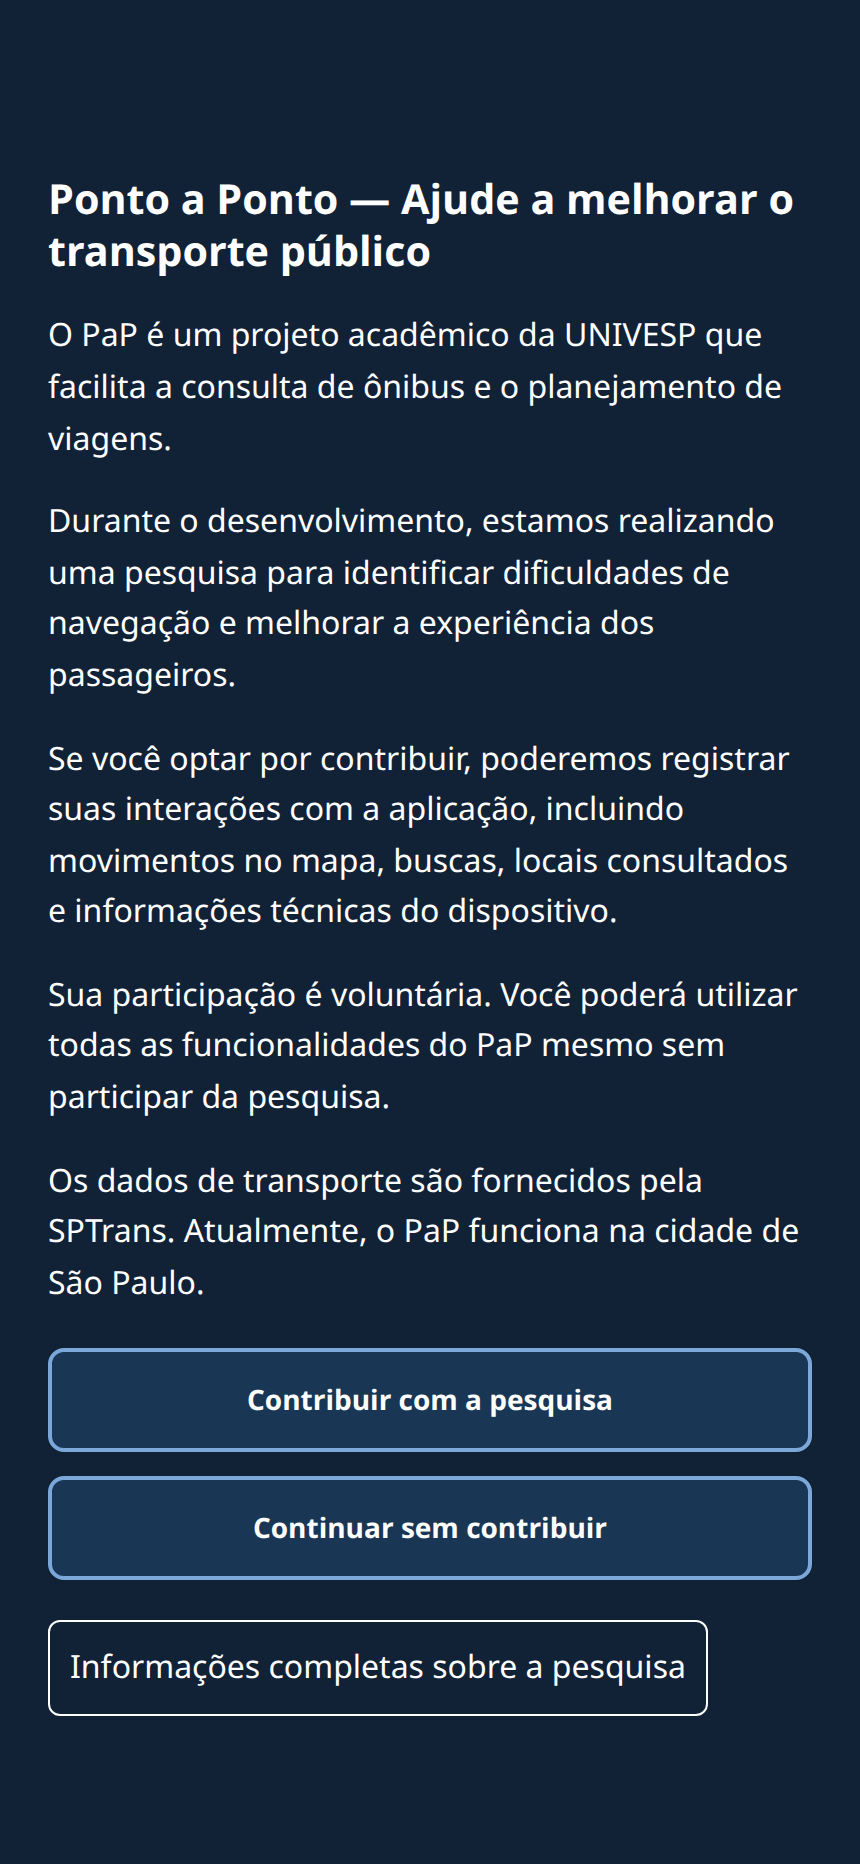
\includegraphics[width=0.80\textwidth,height=0.69\textheight,keepaspectratio]{capturas/2026-10-25/pesquisa-inicial.png}
\caption{Primeiro acesso: participação voluntária na pesquisa e acesso ao transporte sem contribuir.}\label{fig:print-02-informacoes}
\fonte{Captura da aplicação em emulação móvel, revisão 85417bc, 25 out. 2026.}
\end{figure}
O aviso informa a cobertura da SPTrans em São Paulo e apresenta duas escolhas com destaque equivalente. Na captura, foi utilizado um navegador sem decisão anterior; em seguida, escolheu-se continuar sem contribuir. A decisão é persistida localmente com versão do aviso e data, separada dos identificadores de gravação, e pode ser revista nas configurações. Os limites da coleta são discutidos adiante neste capítulo.
\clearpage

\begin{figure}[H]\centering
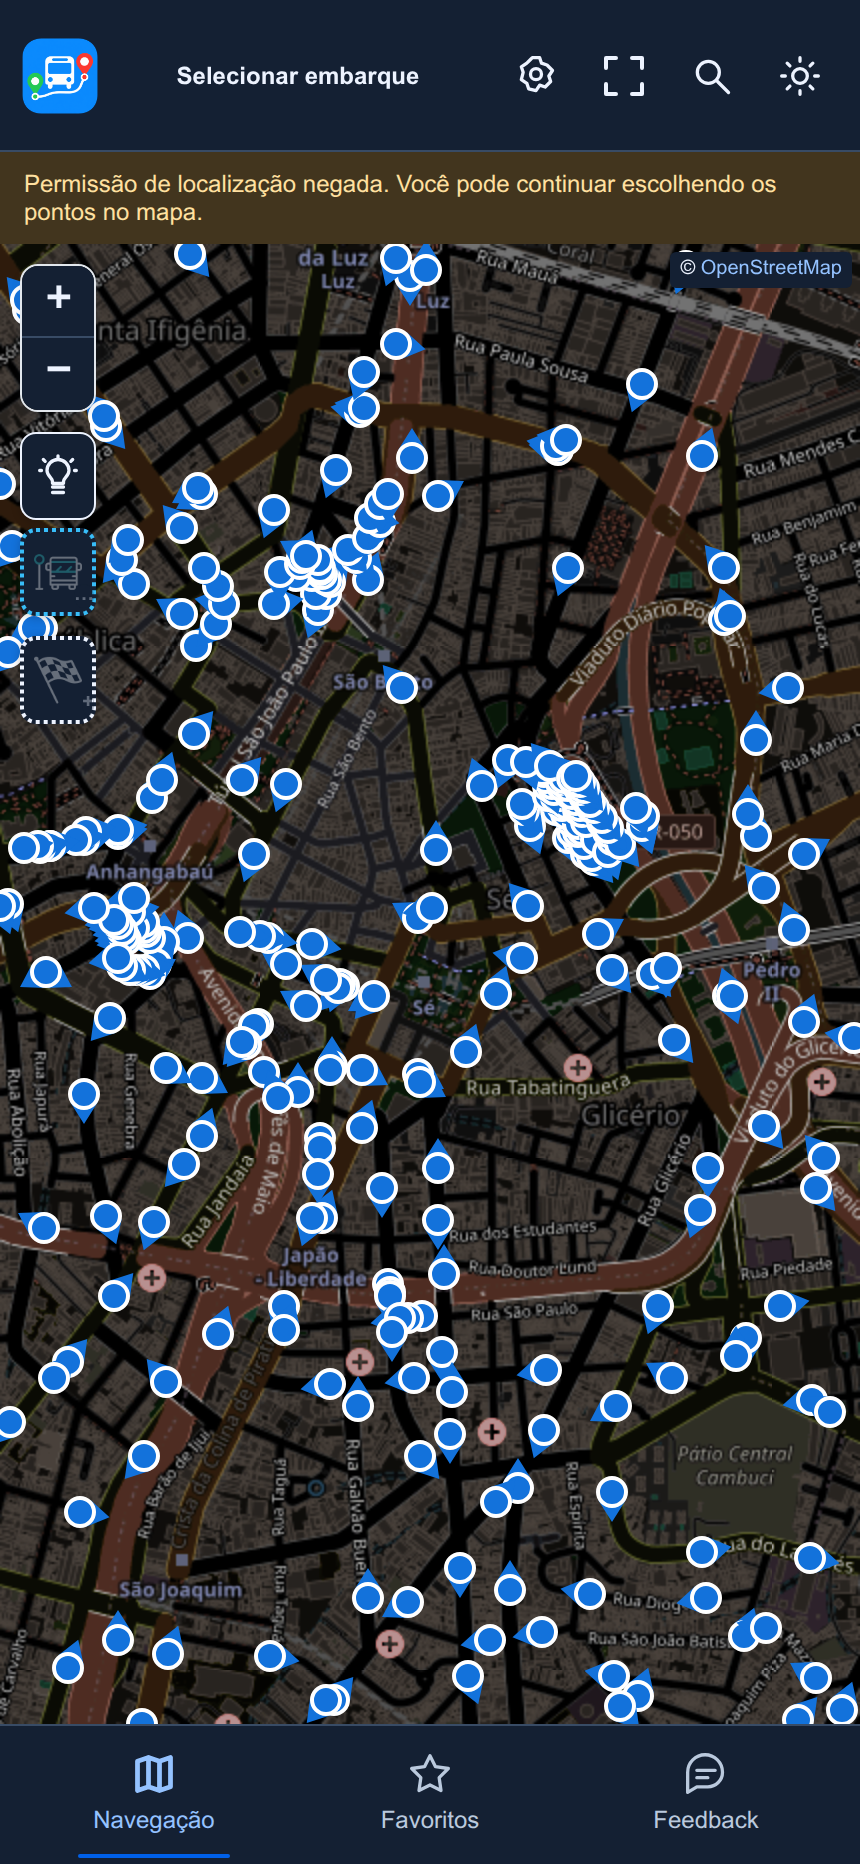
\includegraphics[width=0.43\textwidth,height=0.60\textheight,keepaspectratio]{capturas/2026-10-25-sem-aviso/sem-localizacao.png}\hfill
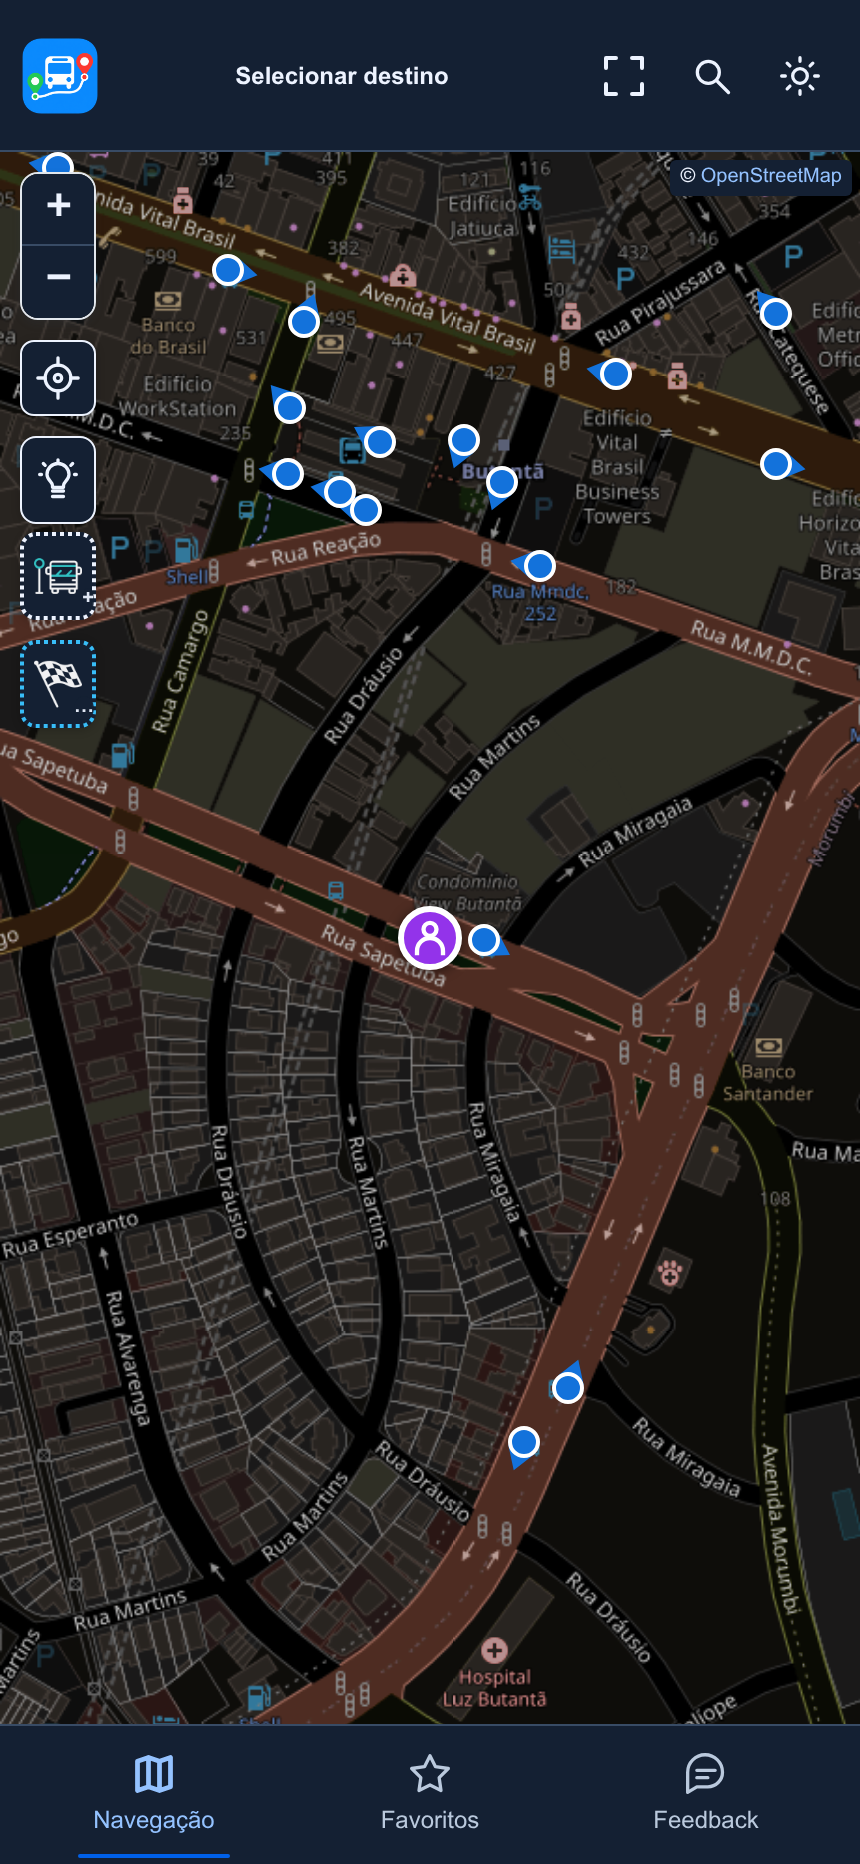
\includegraphics[width=0.43\textwidth,height=0.60\textheight,keepaspectratio]{capturas/2026-10-22/pap-09-localizacao.png}
\caption{Acesso comum após a escolha sobre pesquisa: sem localização autorizada (à esquerda) e com localização simulada como origem (à direita).}\label{fig:print-entrada-comum}
\fonte{Capturas da aplicação em emulação móvel, 25 e 22 out. 2026, respectivamente.}
\end{figure}
Estas telas representam cenários alternativos, não etapas sucessivas. Sem localização disponível e sem parada identificada, a interface solicita o embarque; a captura à esquerda registra a permissão de localização negada no navegador de teste. Com localização disponível, a origem pode ser definida automaticamente e o cabeçalho passa a solicitar o destino. À direita, a posição no Butantã foi simulada para a documentação. Selecionar manualmente um ponto como embarque mantém o mapa aberto para escolher o destino; a entrada pelo link do ponto segue o caminho apresentado a seguir.
\clearpage

\begin{figure}[H]\centering
\begin{minipage}[c]{0.36\textwidth}\centering
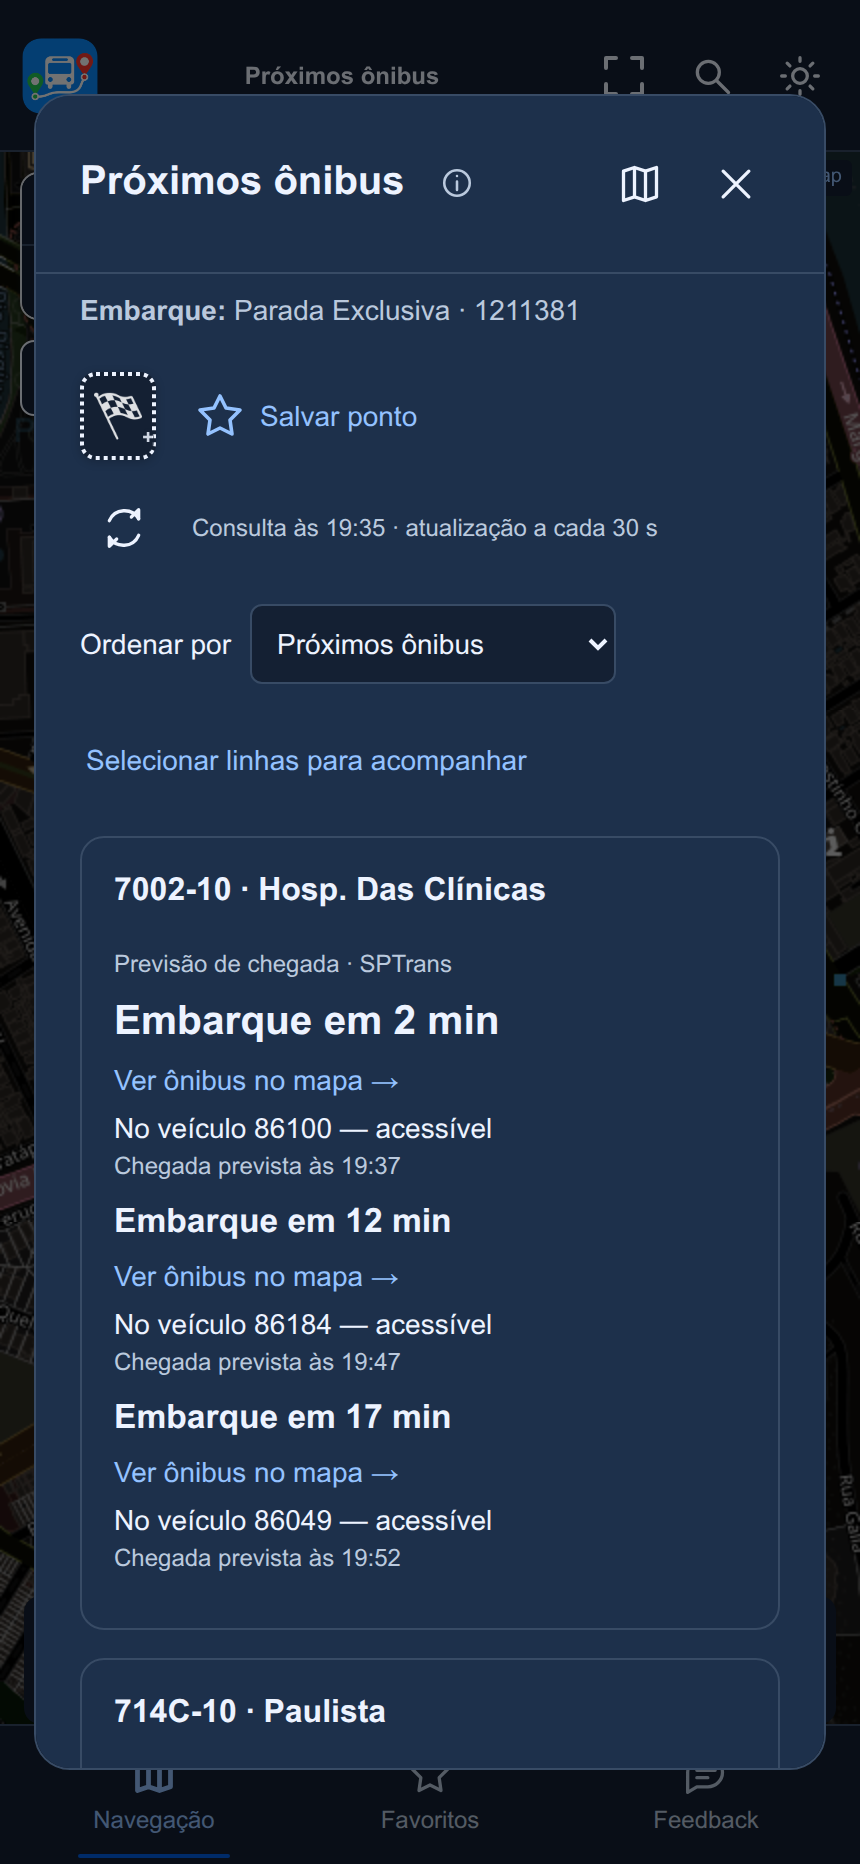
\includegraphics[width=\linewidth]{capturas/2026-10-22/pap-01-embarque.png}
\end{minipage}\hfill
\begin{minipage}[c]{0.60\textwidth}\centering
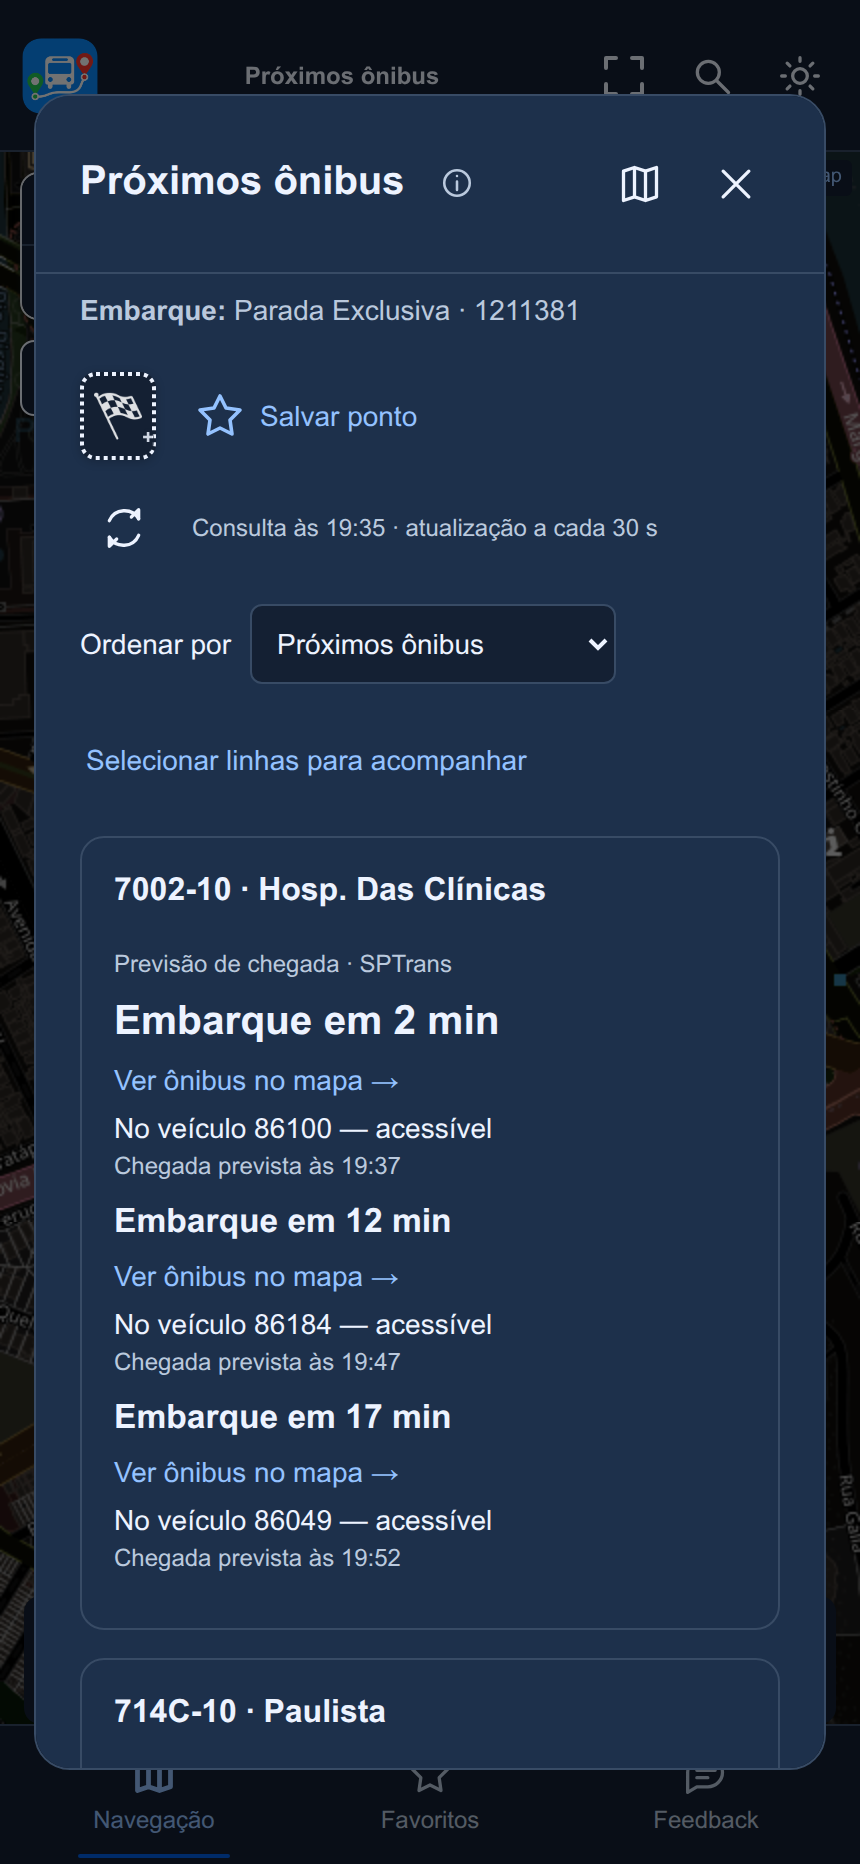
\includegraphics[width=\linewidth,trim=75bp 224bp 70bp 820bp,clip]{capturas/2026-10-22/pap-01-embarque.png}
\small Detalhe ampliado da mesma captura.
\end{minipage}
\caption{Entrada pelo link da parada: próximos ônibus e detalhe das previsões (registro de 22 out. 2026).}\label{fig:print-01-embarque}
\fonte{Captura da aplicação em emulação móvel, 22 out. 2026.}
\end{figure}
Neste registro de 22 de outubro, anterior à reformulação do consentimento, após aceitar o aviso, a consulta foi aberta pelo endereço local da Parada Exclusiva (1211381), no Butantã. Esse acesso reproduz o destino de um QR Code, sem leitura pela câmera. Diferentemente da escolha de embarque no mapa, o painel de próximos ônibus abre automaticamente. O painel distingue previsões operacionais e informações programadas. Os horários são os retornados na captura e não constituem promessa de chegada.
\clearpage

\begin{figure}[H]\centering
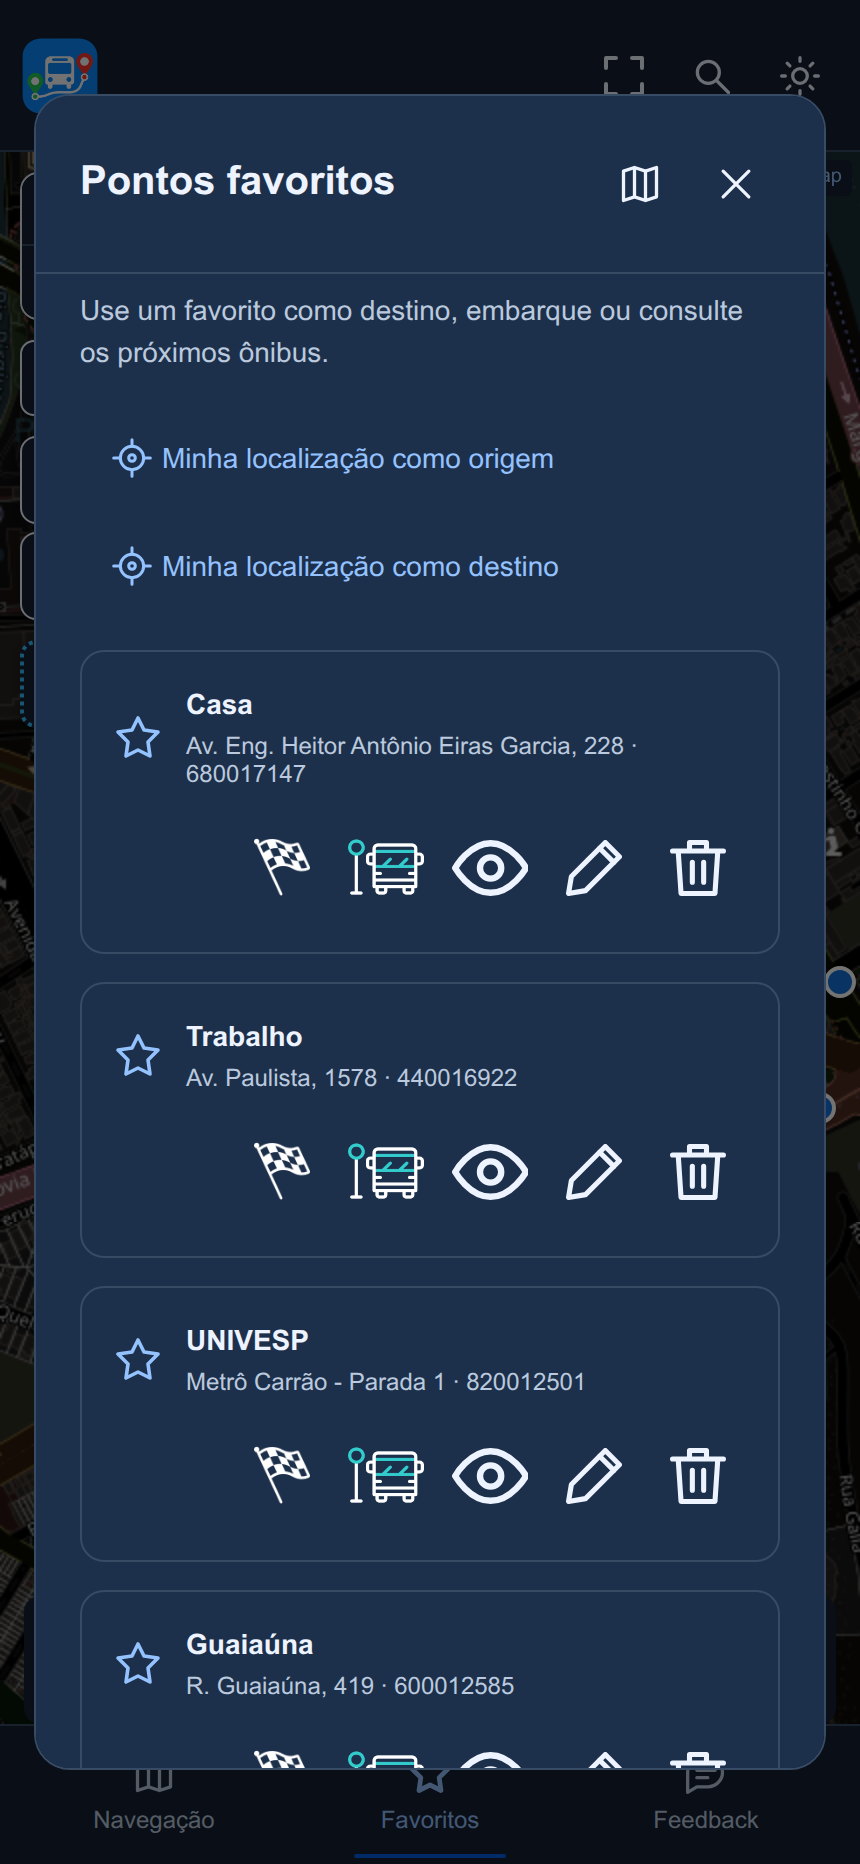
\includegraphics[width=0.80\textwidth,height=0.68\textheight,keepaspectratio]{capturas/2026-10-22/pap-03-destino.png}
\caption{Após fechar a consulta para ver o mapa: favoritos disponíveis para escolher o destino.}\label{fig:print-03-destino}\label{fig:print-07-favoritos}
\fonte{Captura da aplicação em emulação móvel, 22 out. 2026.}
\end{figure}
Na sequência registrada, foi acionado Ver mapa e, em seguida, Favoritos. Os favoritos foram preparados para a documentação com pontos reais e nomes ilustrativos: Casa, Trabalho, UNIVESP e Guaiaúna. Os atalhos permitem escolher destino, embarque ou consulta de próximos ônibus, além de renomear ou remover pontos. Após rolar a lista até a ação de destino de Guaiaúna, sua seleção abre as alternativas da próxima figura; o cadastro dos favoritos é uma preparação da captura, não uma etapa obrigatória do primeiro acesso.
\clearpage

\begin{figure}[H]\centering
\begin{minipage}[c]{0.36\textwidth}\centering
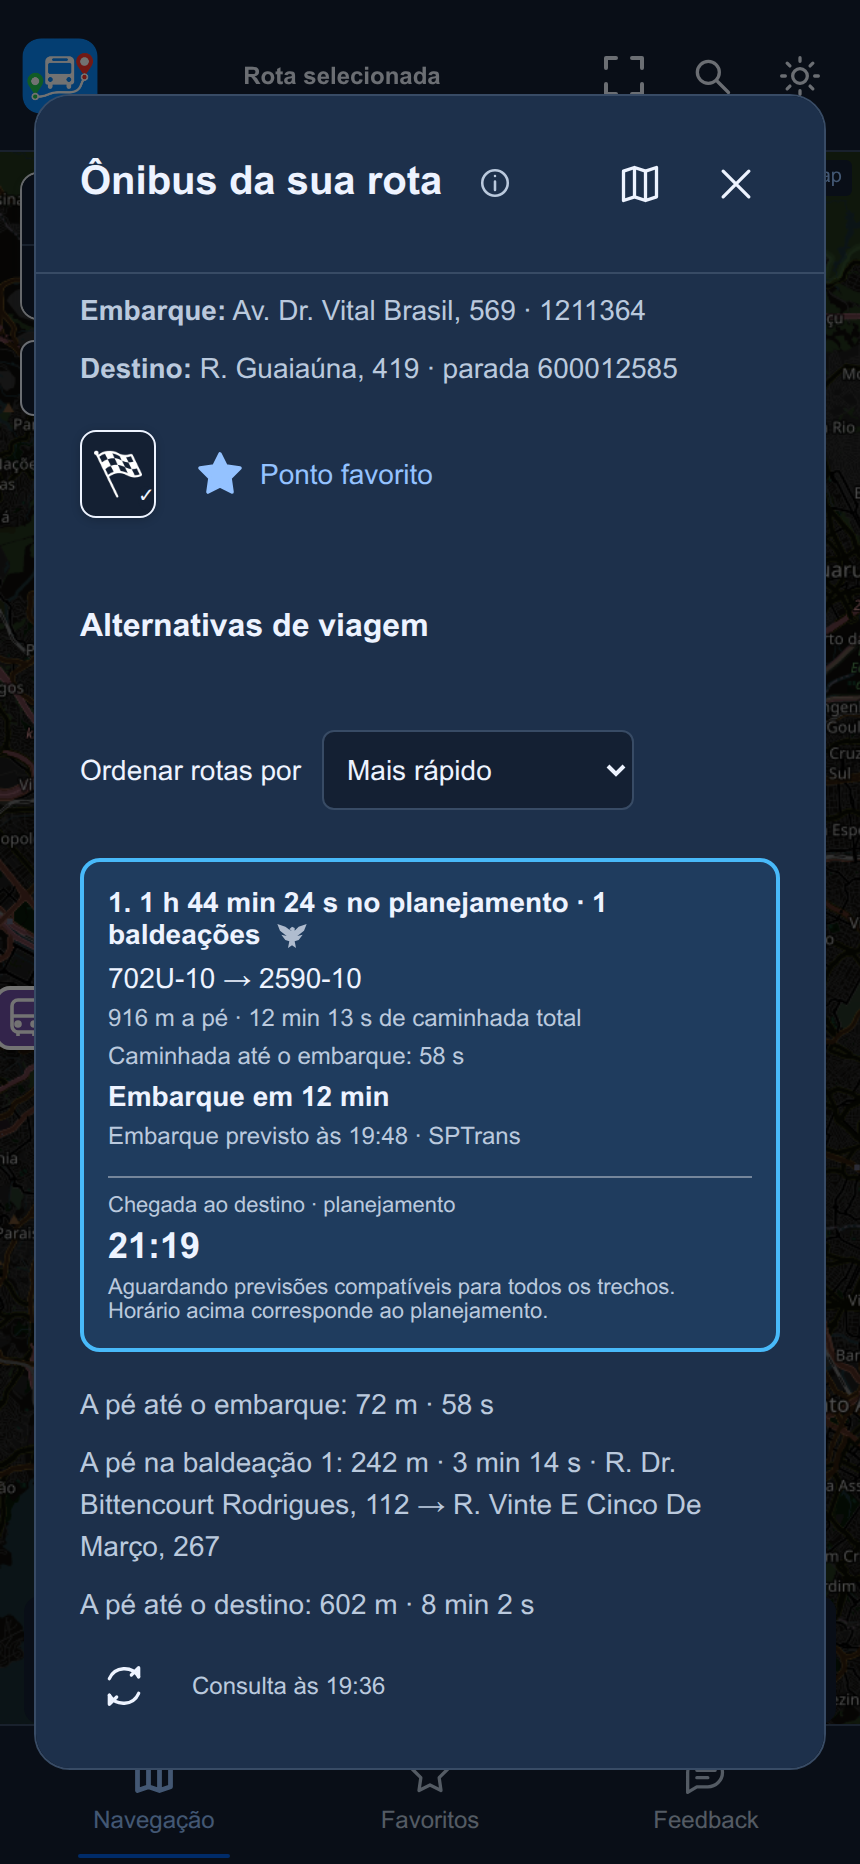
\includegraphics[width=\linewidth]{capturas/2026-10-22/pap-04-alternativas.png}
\end{minipage}\hfill
\begin{minipage}[c]{0.60\textwidth}\centering
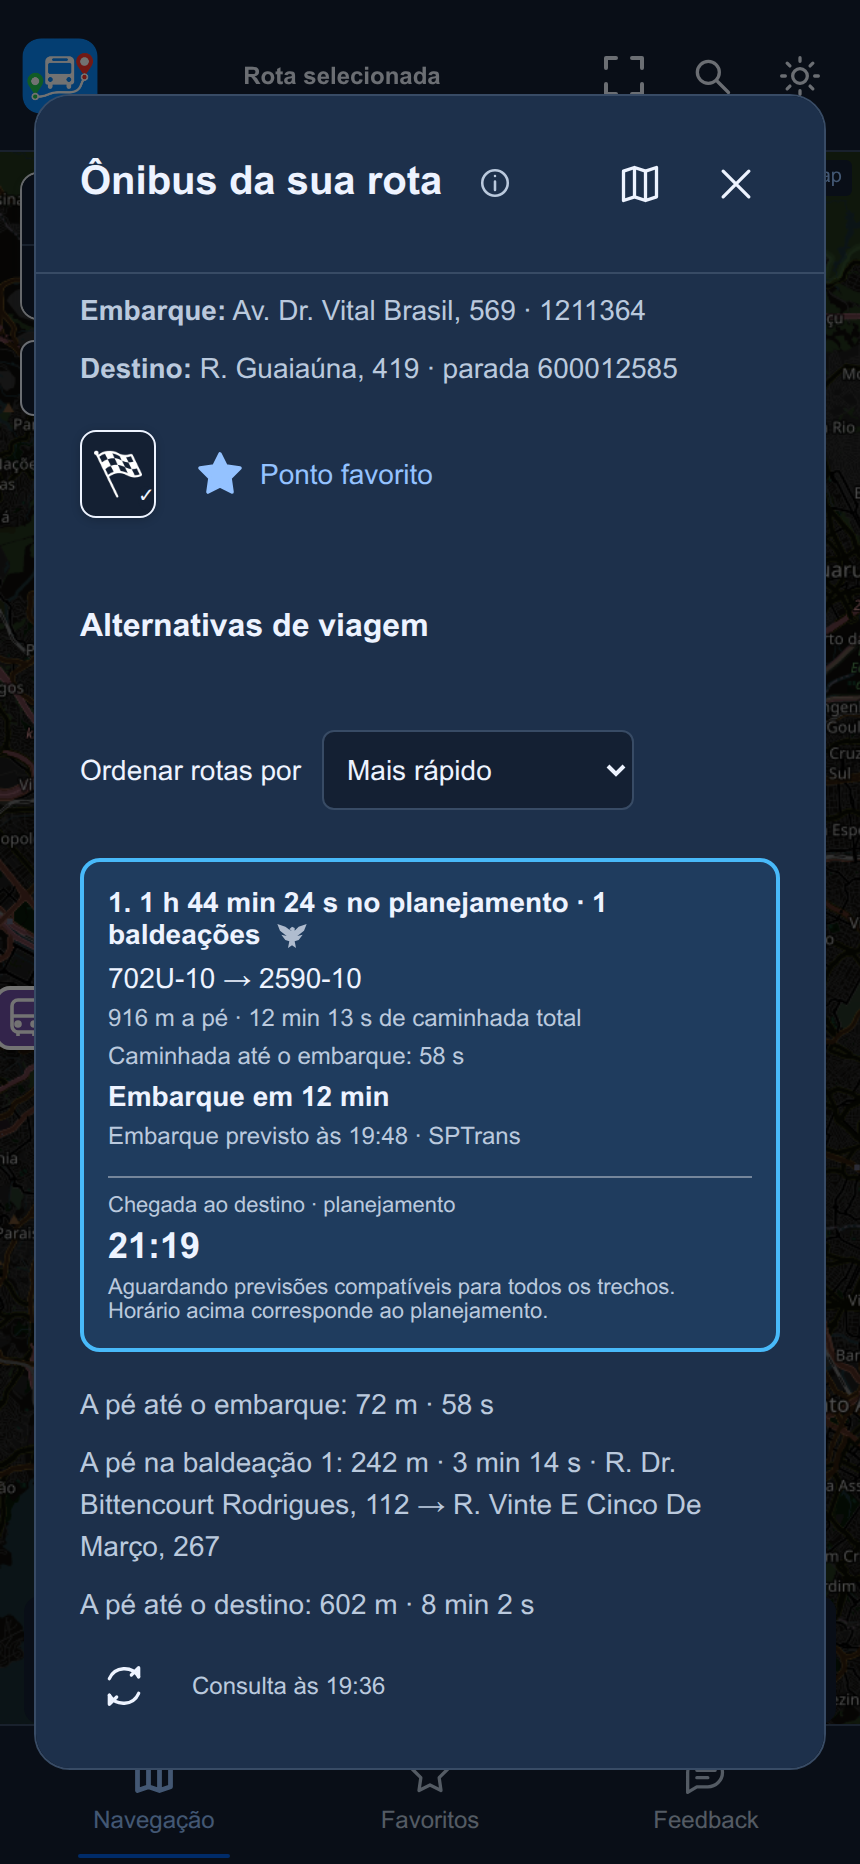
\includegraphics[width=\linewidth,trim=75bp 504bp 70bp 850bp,clip]{capturas/2026-10-22/pap-04-alternativas.png}
\small Detalhe ampliado da mesma captura.
\end{minipage}
\caption{Alternativas de viagem: tela completa e detalhe da alternativa selecionada.}\label{fig:print-04-alternativas}
\fonte{Captura da aplicação em emulação móvel, 22 out. 2026.}
\end{figure}
As capturas integram a mesma sequência registrada no roteiro de captura: acesso à Parada Exclusiva (1211381), retorno ao mapa e seleção de Guaiaúna como destino favorito. O painel de alternativas mostra o embarque do primeiro trecho da rota selecionada, na Av. Dr. Vital Brasil, 569 (1211364), e o destino na Rua Guaiaúna, 419 (600012585). A caminhada de acesso exibida é de 72 m, estimada em 58 s; portanto, o embarque da alternativa difere do ponto usado para iniciar a consulta. O painel apresenta as alternativas calculadas no instante da consulta, com caminhada, baldeações e informações de embarque. Os resultados variam com o horário e com os dados disponíveis.
\clearpage

\begin{figure}[H]\centering
\begin{minipage}[t]{0.48\textwidth}\centering\vspace{0pt}
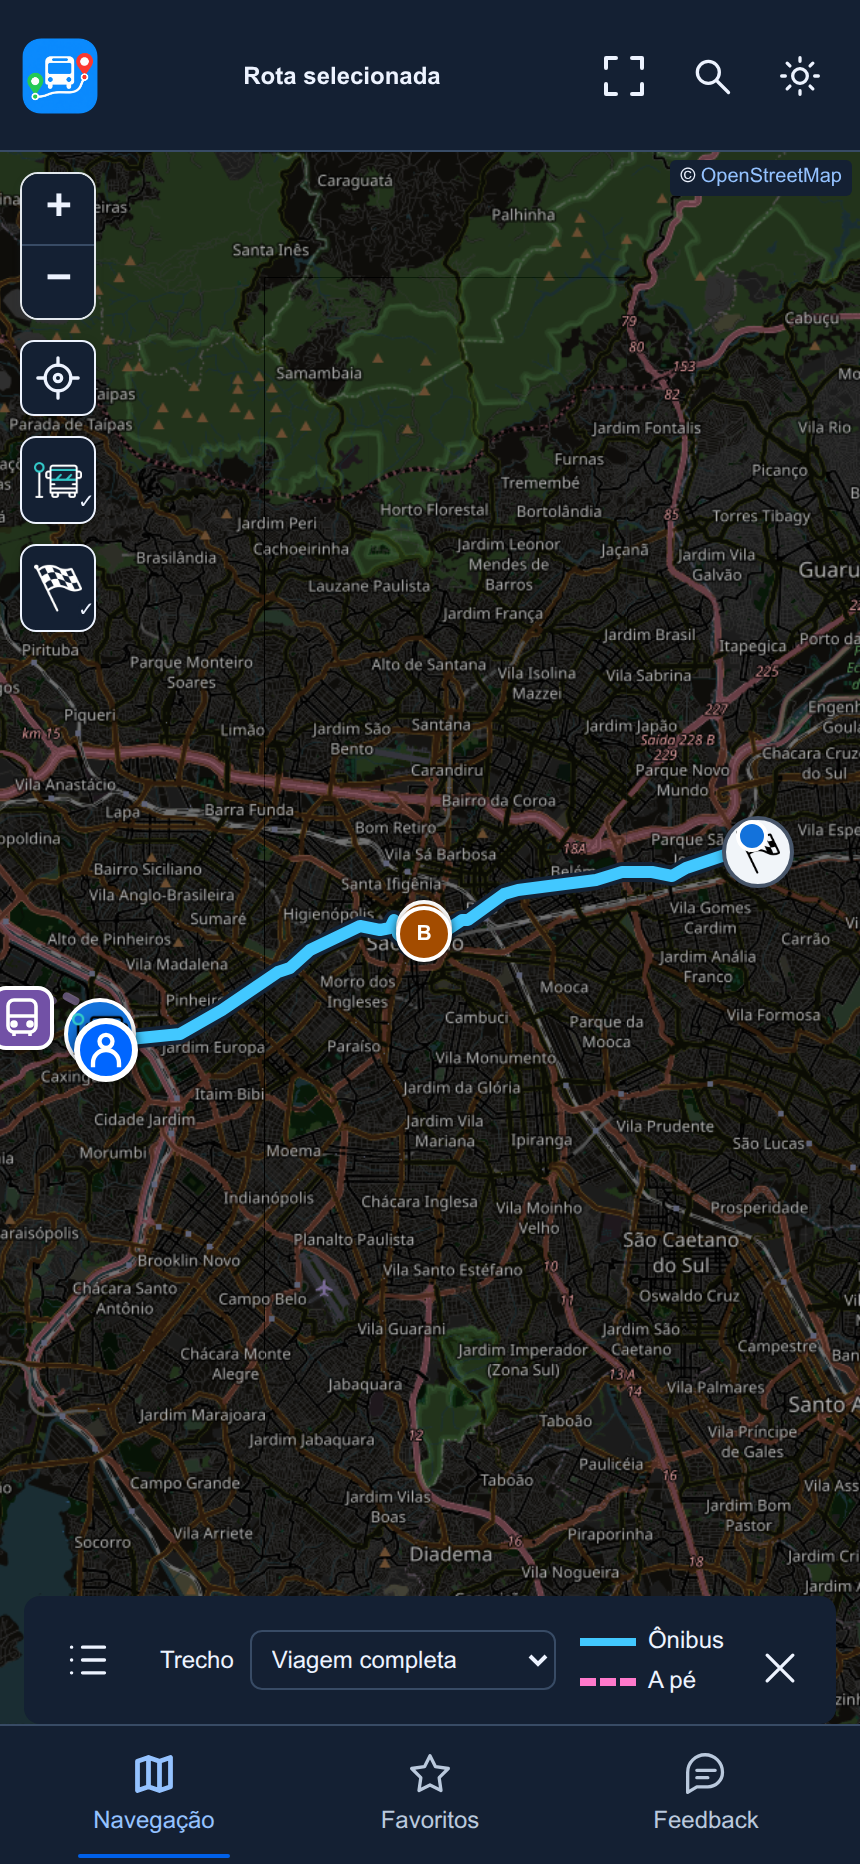
\includegraphics[width=\linewidth,height=0.68\textheight,keepaspectratio]{capturas/2026-10-22/pap-05-viagem-completa.png}
\caption{Viagem completa, com embarque, baldeação e destino.}\label{fig:print-05-viagem-completa}
\end{minipage}\hfill
\begin{minipage}[t]{0.48\textwidth}\centering\vspace{0pt}
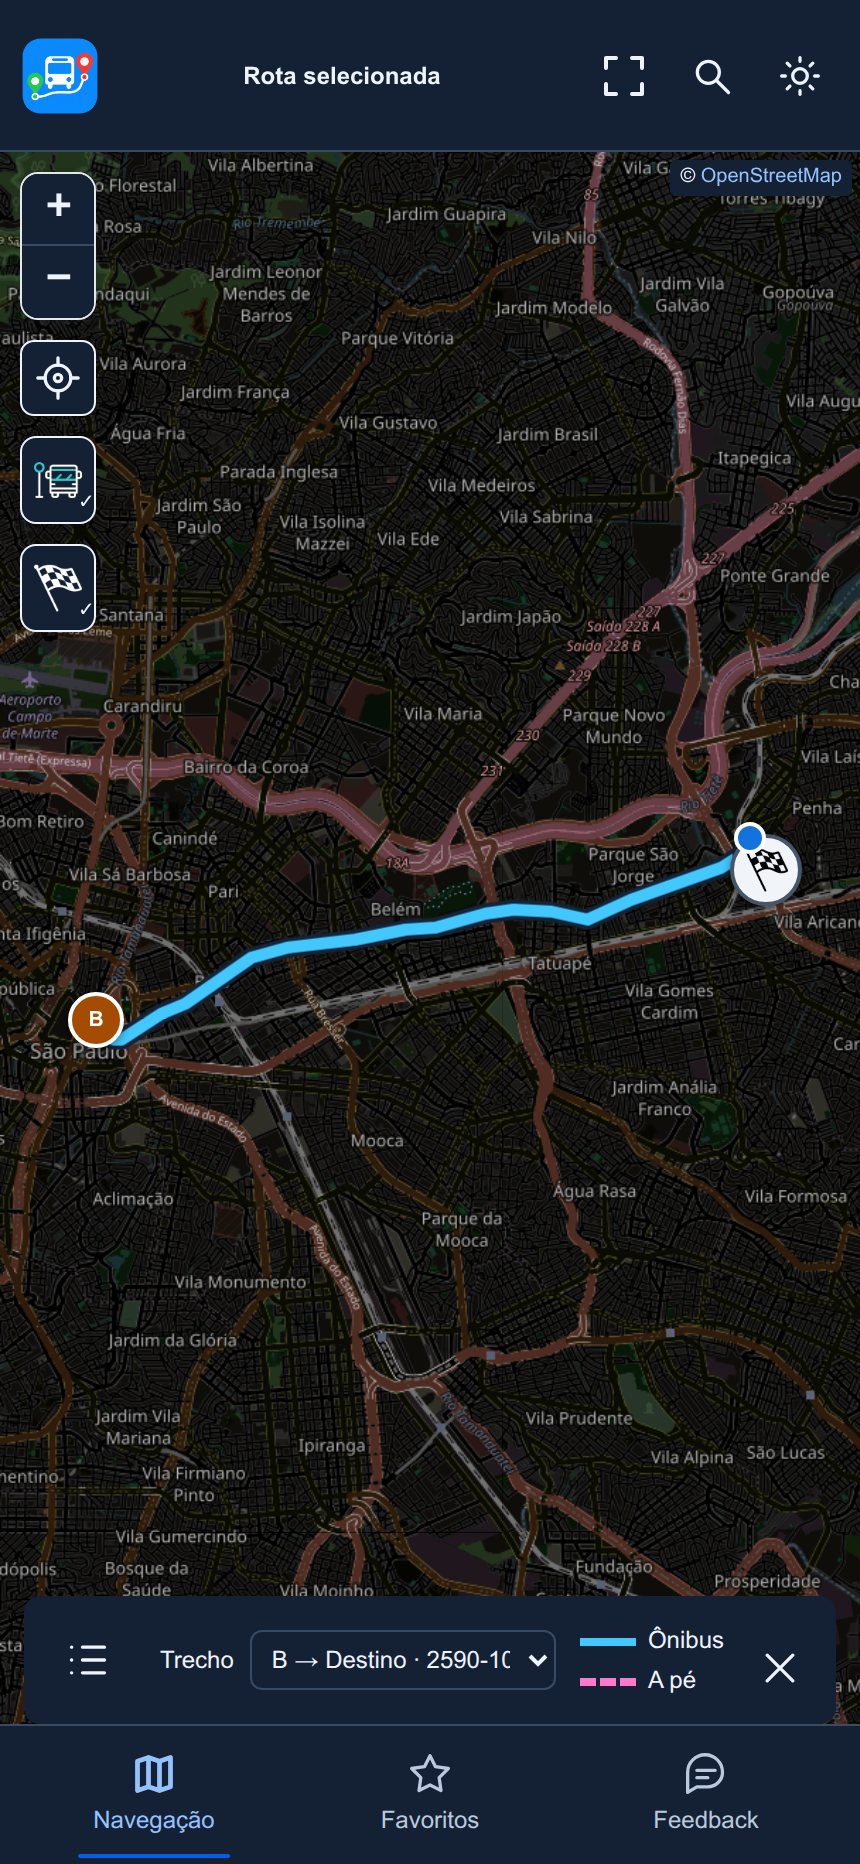
\includegraphics[width=\linewidth,height=0.68\textheight,keepaspectratio]{capturas/2026-10-22/pap-06-ultimo-trecho.png}
\caption{Visualização do último trecho da viagem selecionada.}\label{fig:print-06-ultimo-trecho}
\end{minipage}
\fonte{Capturas da aplicação em emulação móvel, 22 out. 2026.}
\end{figure}
A rota selecionada é representada no mapa, cuja legenda distingue ônibus e caminhada. O controle inferior permite retornar à lista ou examinar um trecho, inclusive a parte final, mantendo a referência da viagem escolhida.
\clearpage

\begin{figure}[H]\centering
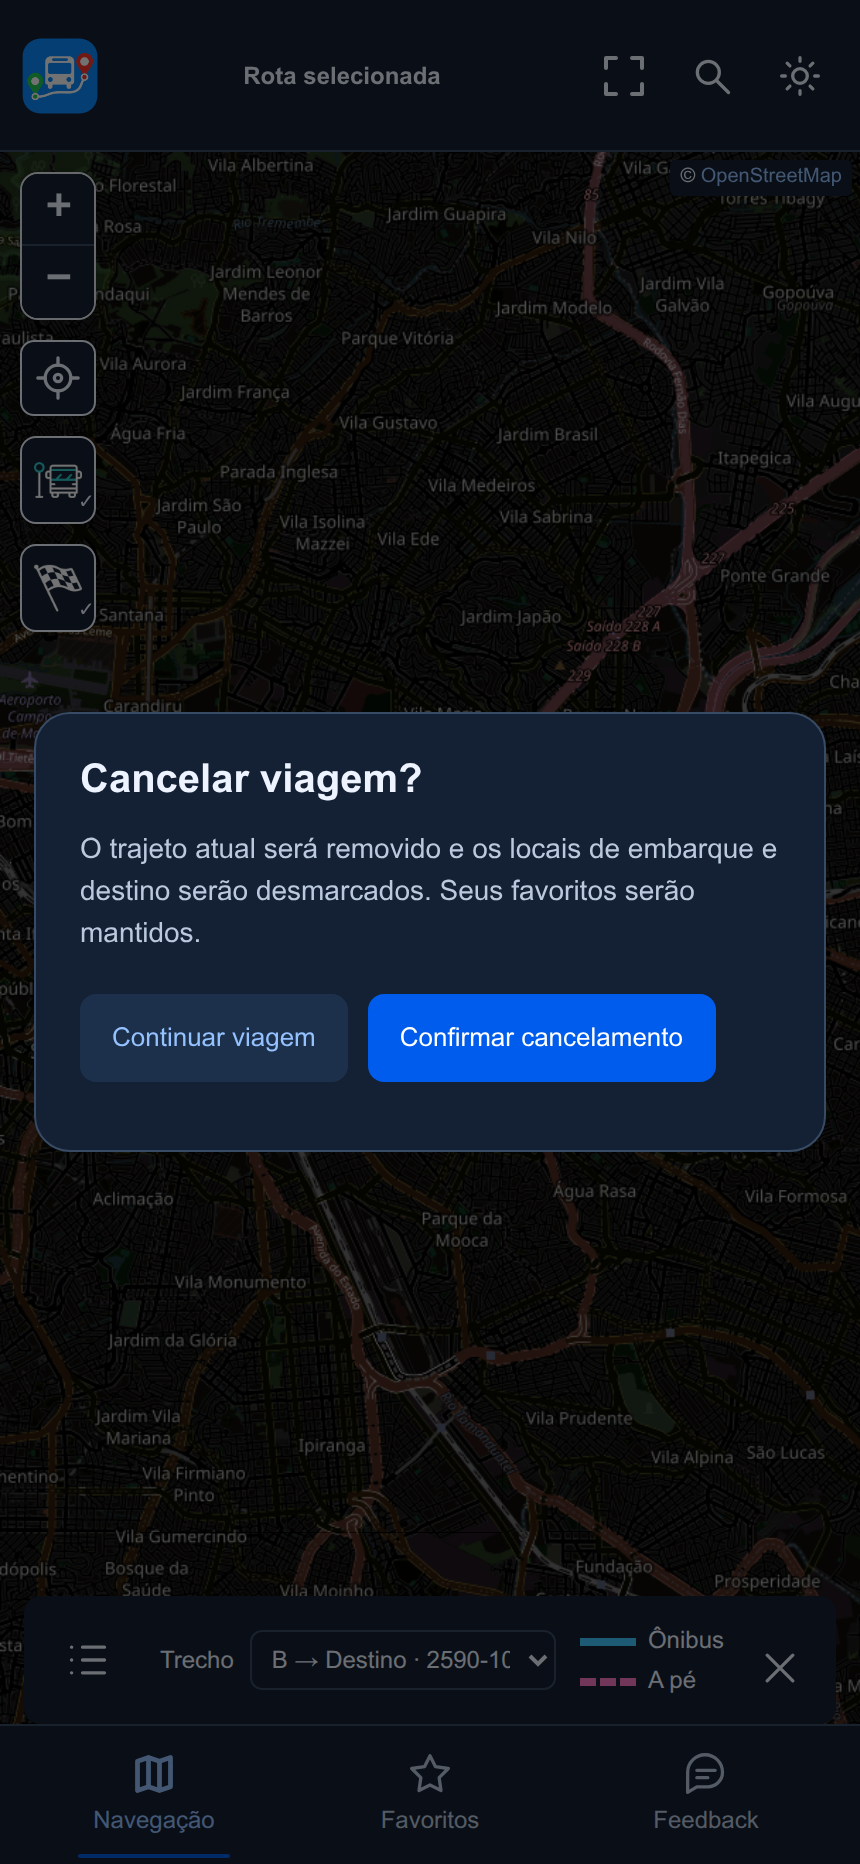
\includegraphics[width=0.80\textwidth,height=0.68\textheight,keepaspectratio]{capturas/2026-10-22/pap-08-confirmacao.png}
\caption{Confirmação antes de cancelar a viagem.}\label{fig:print-08-confirmacao}
\fonte{Captura da aplicação em emulação móvel, 22 out. 2026.}
\end{figure}
O diálogo explica que o trajeto e os locais de embarque e destino serão desmarcados, preservando os favoritos. O passageiro pode continuar a viagem ou confirmar o cancelamento.
\clearpage

\begin{figure}[H]\centering
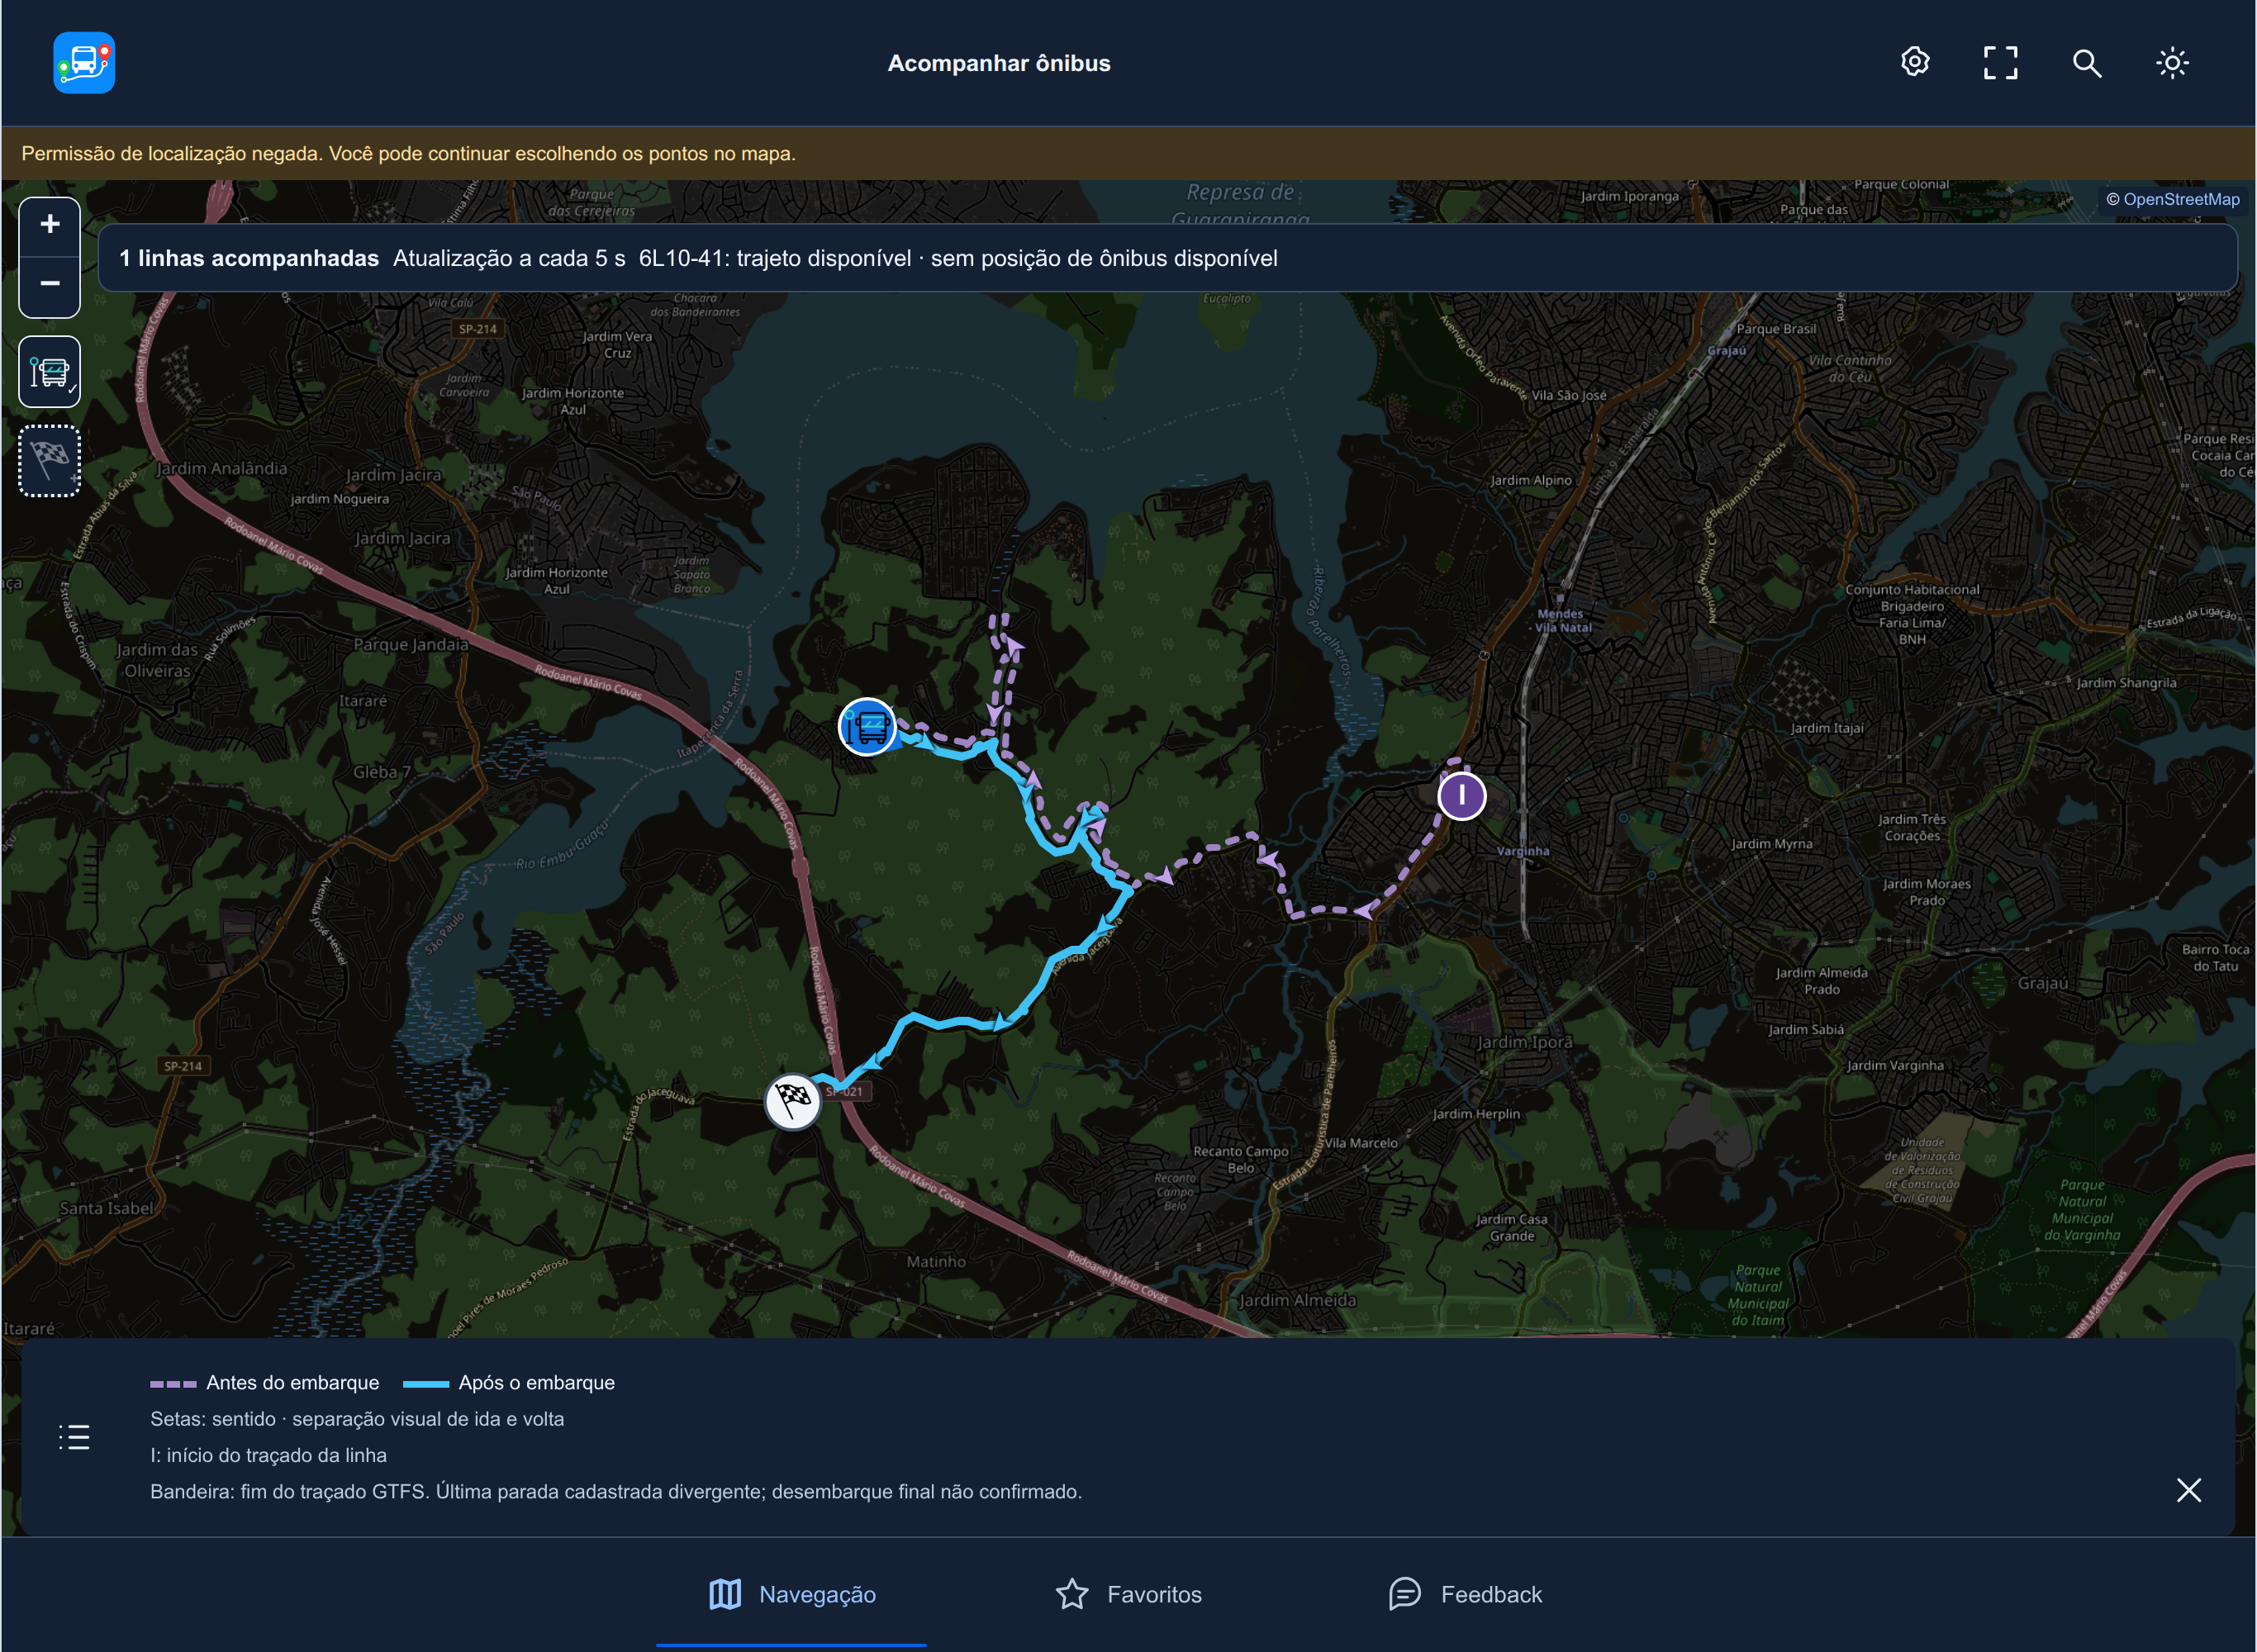
\includegraphics[width=\textwidth,height=0.65\textheight,keepaspectratio]{capturas/2026-10-25-sem-aviso/linha-6L10-completa.png}
\caption{Acompanhamento da linha 6L10-41: traçado completo, setas de sentido e distinção dos trechos.}\label{fig:print-onibus-tempo-real}
\fonte{Captura real da aplicação em navegador de computador, revisão 85417bc com recaptura após ajuste local da interface, 25 out. 2026.}
\end{figure}
Em consulta independente da sequência anterior, foi selecionada a linha 6L10-41, sentido Messiânica, a partir da parada R. Matilde de Lutis Barbosa (5614798). A visualização não exige posição de ônibus disponível: nesta captura, o estado operacional informa sua ausência. O início do traçado aparece com ``I''; a bandeira indica seu final com ressalva sobre o cadastro da última parada. As setas mostram o sentido e o pequeno afastamento visual permite distinguir passagens opostas pela mesma via. O caso que motivou essa alteração é descrito na avaliação interna de uso.
\clearpage

\begin{figure}[H]\centering
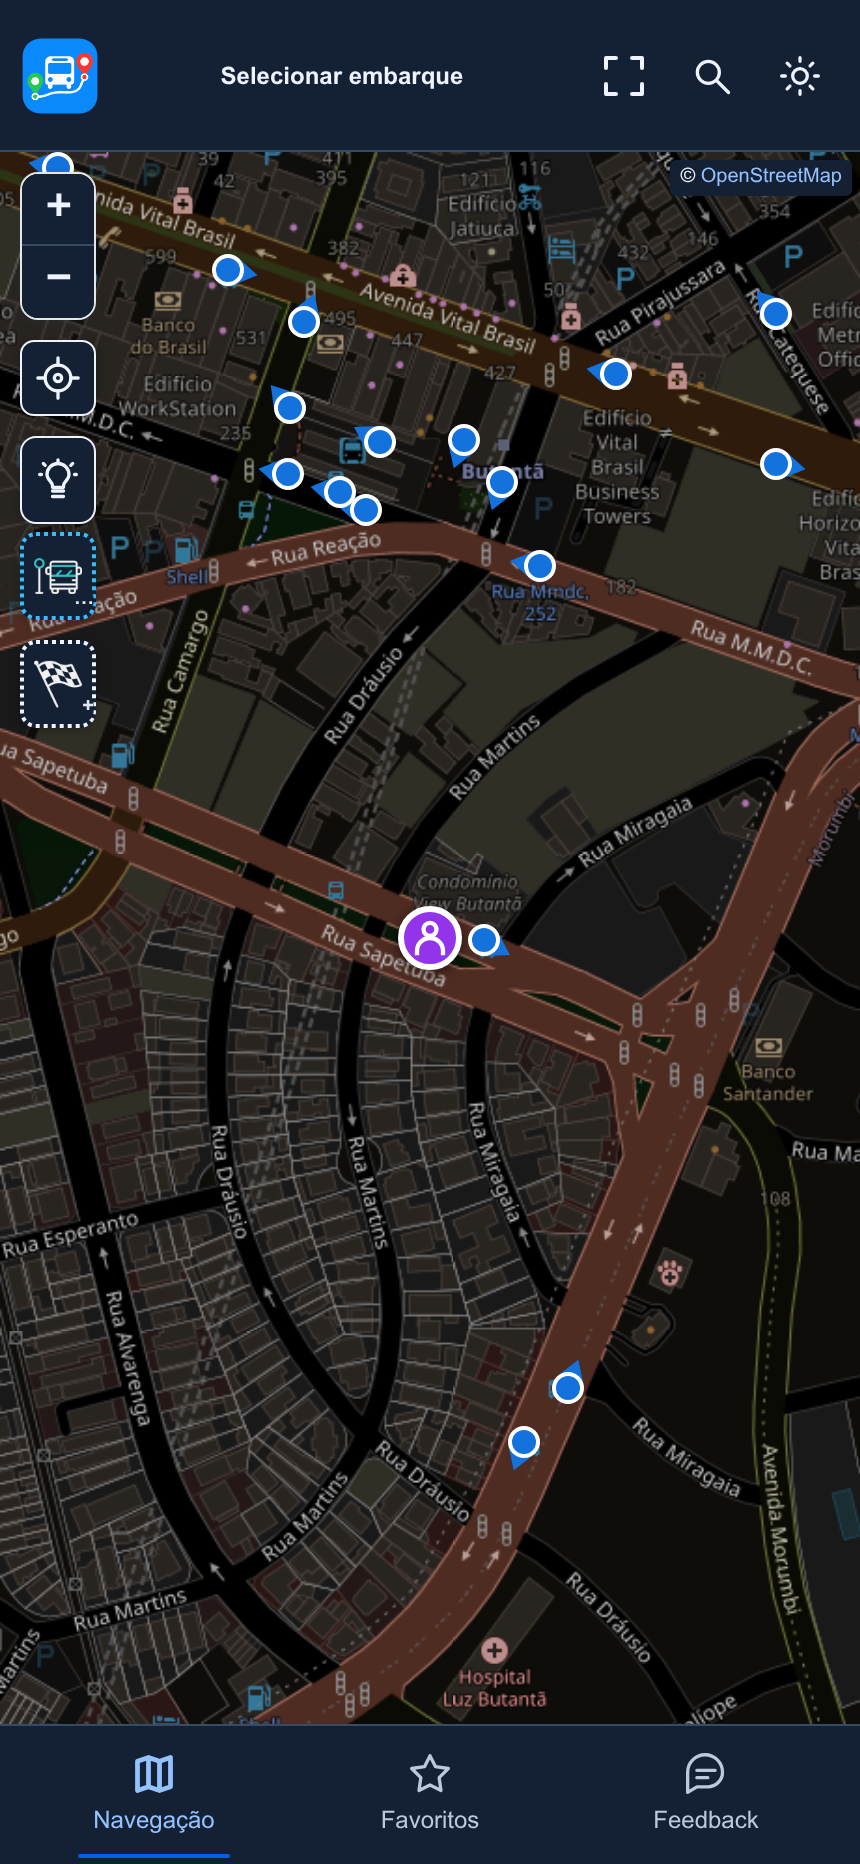
\includegraphics[width=0.80\textwidth,height=0.60\textheight,keepaspectratio]{capturas/2026-10-22/pap-10-alterar-embarque.png}
\caption{Cenário alternativo: ativação da seleção manual de embarque a partir da localização simulada.}\label{fig:print-localizacao}
\fonte{Capturas da aplicação em emulação móvel, 22 out. 2026.}
\end{figure}
Esta captura retoma o cenário de localização simulada, independentemente da viagem por Guaiaúna. Após acionar Selecionar embarque, o marcador roxo permanece como referência da localização e o mapa aguarda a escolha manual da origem. O controle lateral permite escolher uma parada de embarque no mapa. O cabeçalho utiliza a expressão Selecionar embarque; a navegação inferior inclui o acesso ao feedback.
\clearpage

\begin{figure}[H]\centering
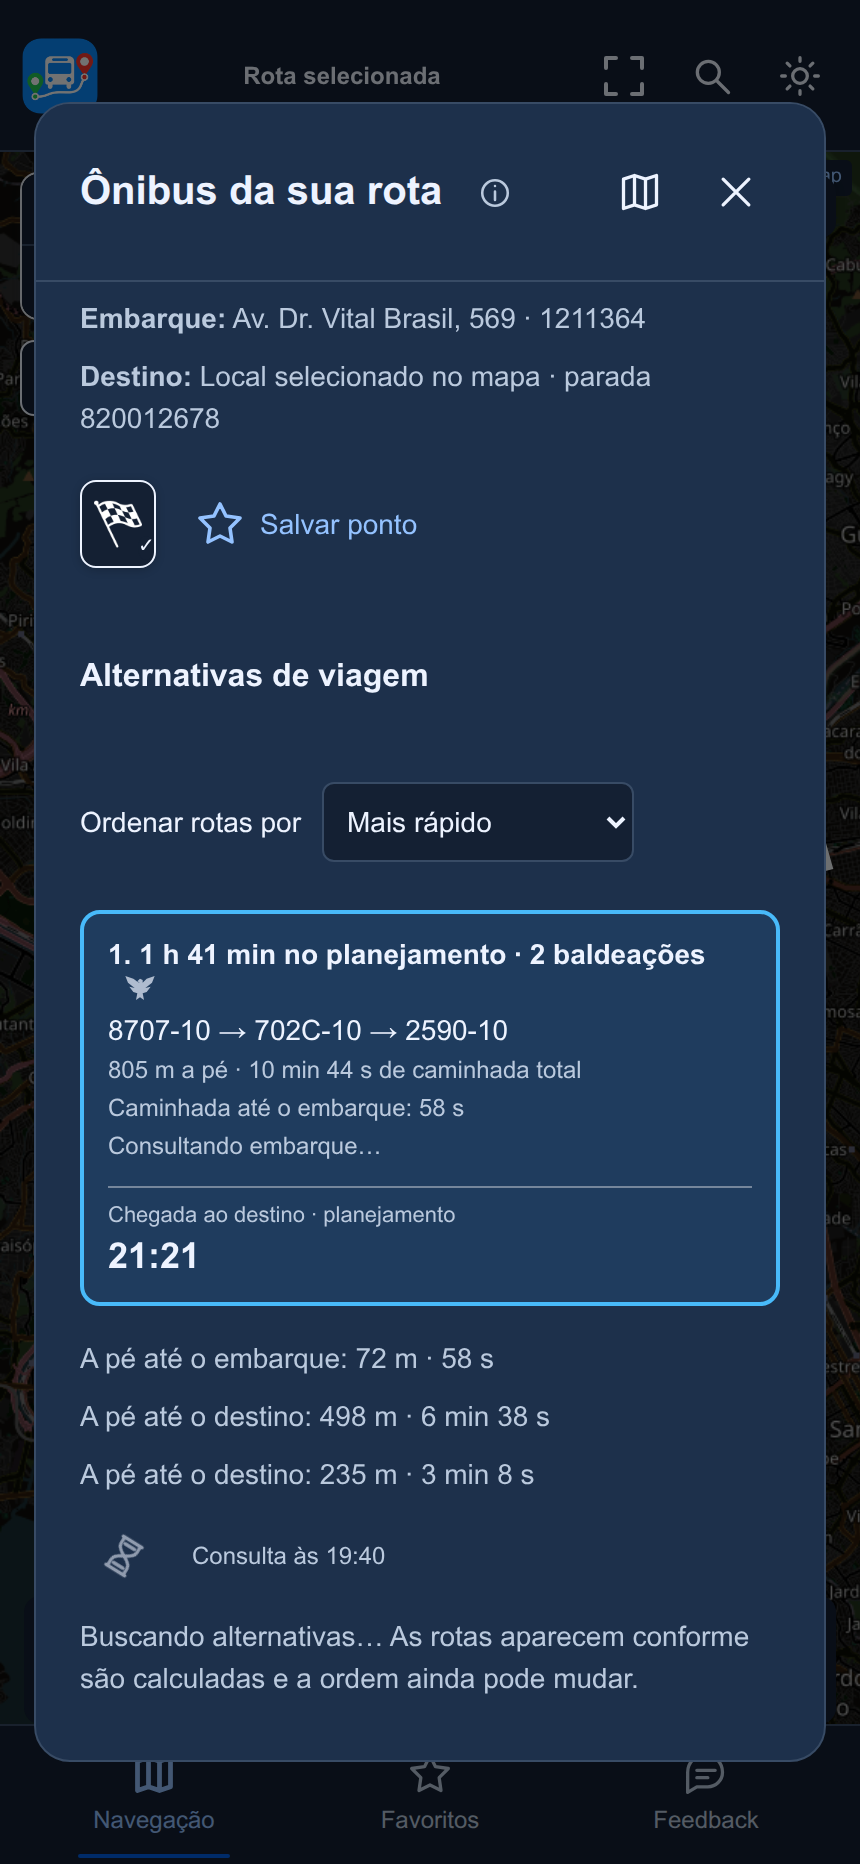
\includegraphics[width=0.80\textwidth,height=0.68\textheight,keepaspectratio]{capturas/2026-10-22/pap-12-destino-livre.png}
\caption{Destino definido por toque prolongado no mapa.}\label{fig:print-destino-livre}
\fonte{Captura da aplicação em emulação móvel, 22 out. 2026.}
\end{figure}
Em um novo acesso pelo link da Parada Exclusiva, após aceitar o aviso e acionar Ver mapa, a busca por coordenadas centralizou a região desejada e o toque prolongado definiu um local de destino. O painel apresenta alternativas progressivamente e, no instante capturado, ainda consulta informações de embarque. A imagem não representa o encerramento de todas as consultas.
\clearpage

\begin{figure}[H]\centering
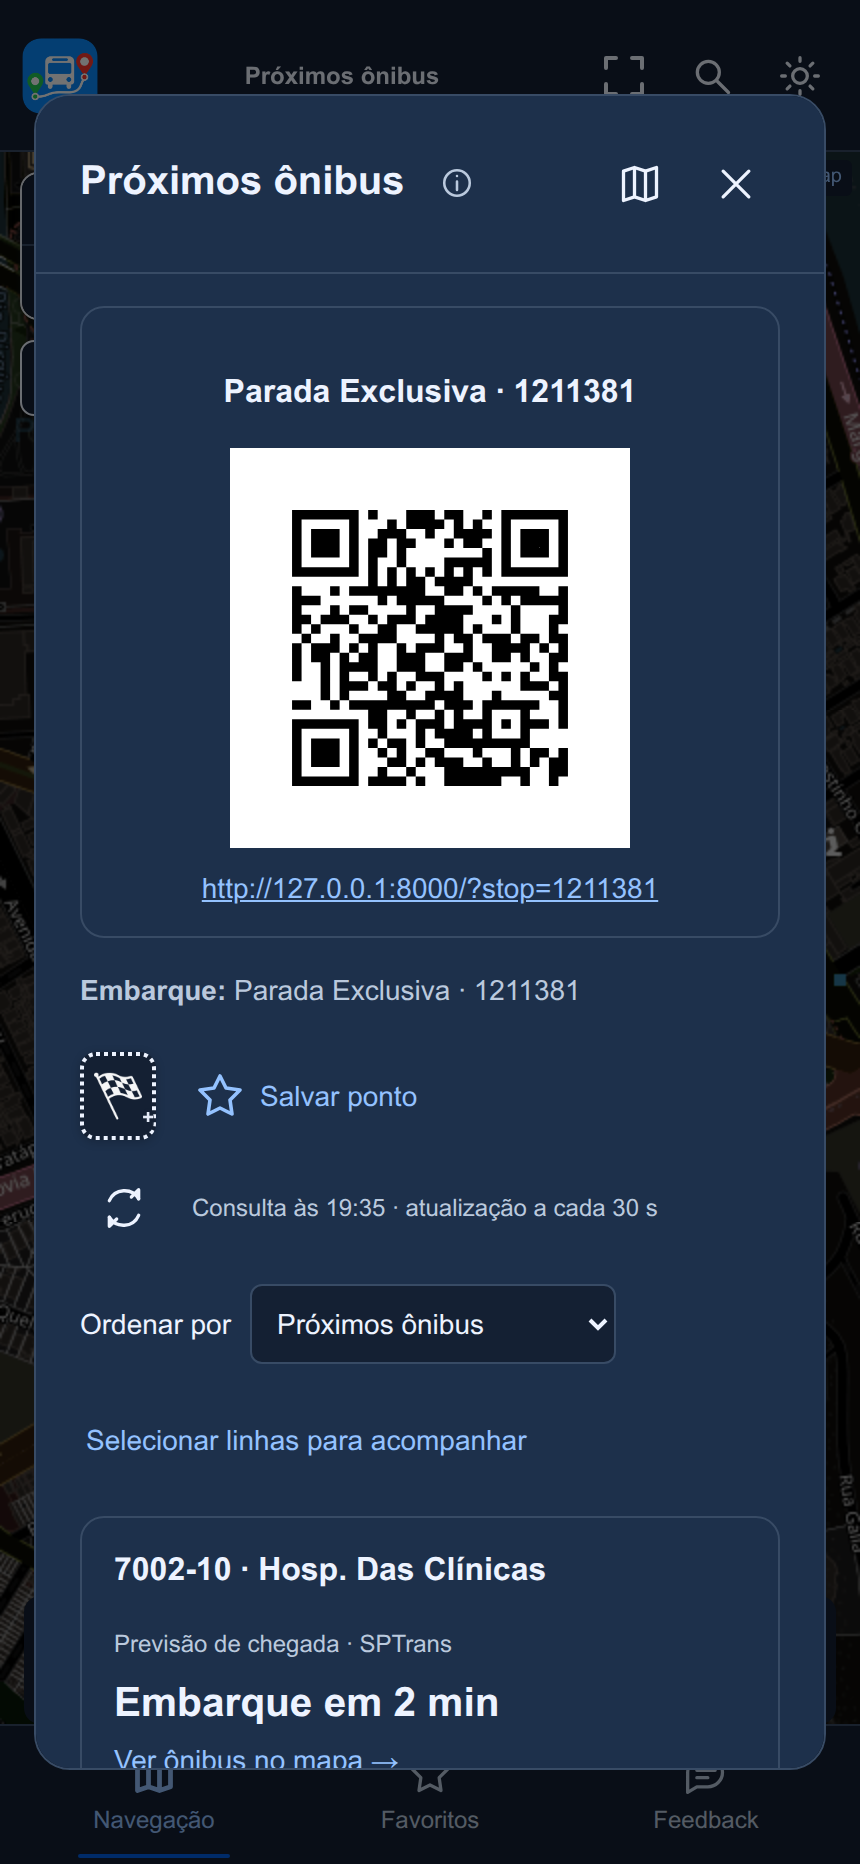
\includegraphics[width=0.80\textwidth,height=0.68\textheight,keepaspectratio]{capturas/2026-10-22/pap-14-qr-atual.png}
\caption{Informações da parada e QR Code de acesso à consulta.}\label{fig:print-qr-atual}
\fonte{Captura da aplicação em emulação móvel, 22 out. 2026.}
\end{figure}
Como recurso auxiliar, o botão Informações do ponto abre esta tela durante a consulta de próximos ônibus. Ela não é uma etapa posterior ao cancelamento ou ao destino por toque prolongado. A tela utiliza o identificador 1211381 e o endereço local de desenvolvimento. A captura documenta a geração do QR Code; não demonstra leitura física pela câmera. Para uso externo, é necessário um endereço HTTPS acessível aos passageiros.
\clearpage



\section{Escopos da solução e níveis de cobertura}\label{sec:cobertura-revisada}
A evolução do PaP deve ser lida por fonte e por versão. A Tabela~\ref{tab:cenarios-revisados} distingue o demonstrador histórico da integração efetivamente programada; a Tabela~\ref{tab:niveis-cobertura} define o que cada medida permite concluir.
\begingroup\small\SingleSpacing\setlength{\parskip}{0pt}\setlength{\tabcolsep}{4pt}
\begin{longtable}{>{\raggedright\arraybackslash}p{2.7cm}p{6.0cm}p{6.0cm}}
\caption{Comparação das três etapas do projeto.}\label{tab:cenarios-revisados}\\\hline
Etapa & Fonte e entrega & Limite\\\hline\endfirsthead
\hline Etapa & Fonte e entrega & Limite\\\hline\endhead\hline\endfoot
Mauá histórico & Catálogo público, coordenadas parcialmente inferidas e demonstração de horários/veículos em simulação identificada. & Não comprova programação ou operação dos ônibus municipais.\\[4pt]
SPTrans original & GTFS de ônibus e integração ferroviária; 22.274 identificadores no censo de 1/11; Olho Vivo para posições/previsões compatíveis. & Calendário e estimativas condicionam as rotas; previsão depende da API. Não é a rede municipal de Mauá.\\[4pt]
ARTESP em 2/11 & Mais 25.105 registros no cadastro combinado (47.379); em Mauá, 337 paradas, 16 linhas/variantes, conexões com trilhos. & Programação metropolitana de 2026; não integra toda a rede municipal nem demonstra realização da viagem.\\
\end{longtable}
\fonte{Auditorias de 1 e 2 nov. 2026; fontes e procedimentos nos Apêndices~\ref{ap:importacao} e~\ref{ap:rotas}.}
\begin{longtable}{>{\raggedright\arraybackslash}p{2.5cm}p{6.1cm}p{6.1cm}}
\caption{Quatro níveis de cobertura e seus denominadores.}\label{tab:niveis-cobertura}\\\hline
Nível & Evidência existente & O que não mede\\\hline\endfirsthead
\hline Nível & Evidência existente & O que não mede\\\hline\endhead\hline\endfoot
Cadastral & Identificadores, coordenadas, linhas e sequências importadas. Recorte de 337 paradas ARTESP em Mauá, mais três estações ferroviárias separadas. & Percentual da população atendida, estado físico da parada ou completude da rede municipal.\\[4pt]
Estrutural & Em 1/11, 494.451.148 de 496.108.802 pares dirigidos distintos com alternativa materializada (99,666\%), no universo de 22.274 paradas anterior à ARTESP. & Probabilidade de encontrar uma viagem, disponibilidade por horário ou nova cobertura conjunta após 2/11.\\[4pt]
Temporal & Calendários, horários e acessos avaliados para uma consulta; viagens ARTESP distintas em 3, 7 e 8/11 e 12 consultas representativas. & Serviço em todos os horários, feriados não registrados ou datas além da vigência.\\[4pt]
Operacional & Posições/previsões SPTrans quando retornadas e associadas com segurança; não há comprovação de circulação pela simples existência de uma rota GTFS. & Execução real de viagens ARTESP/ferroviárias, pontualidade e viabilidade física de todos os acessos.\\
\end{longtable}
\fonte{Síntese do grupo a partir dos censos e da validação temporal; não se convertem denominadores entre níveis.}
\endgroup
Dos 1.657.654 pares sem materialização, 1.313.444 têm explicação pelas regras examinadas; 344.210 seguem sem causa esclarecida. A política inicial bloqueia 50 origens de término, apesar da caminhada externa verificada. Oito destinos excedem o encaixe pedestre de 20 m e um excede a caminhada de 1.000 m. Isso não comprova erro do GTFS nem inacessibilidade física (Seção~\ref{sec:atualizacao-20261101}).

\section{Desempenho: distribuições e comparação pareada}\label{sec:desempenho-revisado}
O ensaio de 1 de novembro repetiu 3.264 consultas por versão, com 32 processos e partidas simuladas em 3 de novembro às 02h, 08h e 14h. Mede o tempo local até a primeira rota, sem HTTP, túnel, rede externa ou renderização no celular. As 1.637 consultas com rota nas duas versões constituem o conjunto pareado: a mediana \textbf{piorou de 0,282 para 0,599 s}, enquanto o P95 caiu de 5,698 para 5,143 s e o maior tempo observado de 10,712 para 5,936 s. A redução da cauda não representa ganho generalizado.
\begin{table}[H]\centering\small
\caption{Desfechos de todas as consultas do ensaio, antes do pareamento.}\label{tab:estados-benchmark}
\begin{tabular}{>{\raggedright\arraybackslash}p{8cm}rr}\hline
Estado & Antes & Depois\\\hline
Primeira rota & 1.652 & 1.728\\
Dependência externa não medida & 936 & 839\\
Busca encerrada sem rota & 676 & 697\\\hline
Total & 3.264 & 3.264\\\hline
\end{tabular}
\fonte{Medições individuais de 1 nov. 2026. ``Sem rota'' descreve o encerramento observado, não inexistência de caminho na rede real.}
\end{table}
A Tabela~\ref{tab:estados-benchmark} impede interpretar os sucessos pareados como todos os casos do experimento. Houve 91 novos sucessos e 15 sucessos anteriores não reproduzidos, dos quais 12 dependiam de chamada externa e três encerraram com busca limitada. A amostra inclui casos problemáticos deliberadamente e não estima taxa de atendimento municipal. A documentação de parâmetros, resultados por custo e lacunas de reprodução permanece na Seção~\ref{sec:atualizacao-20261101}. Custo ponderado de transferência não equivale sempre ao número físico de baldeações.

\begin{figure}[H]\centering
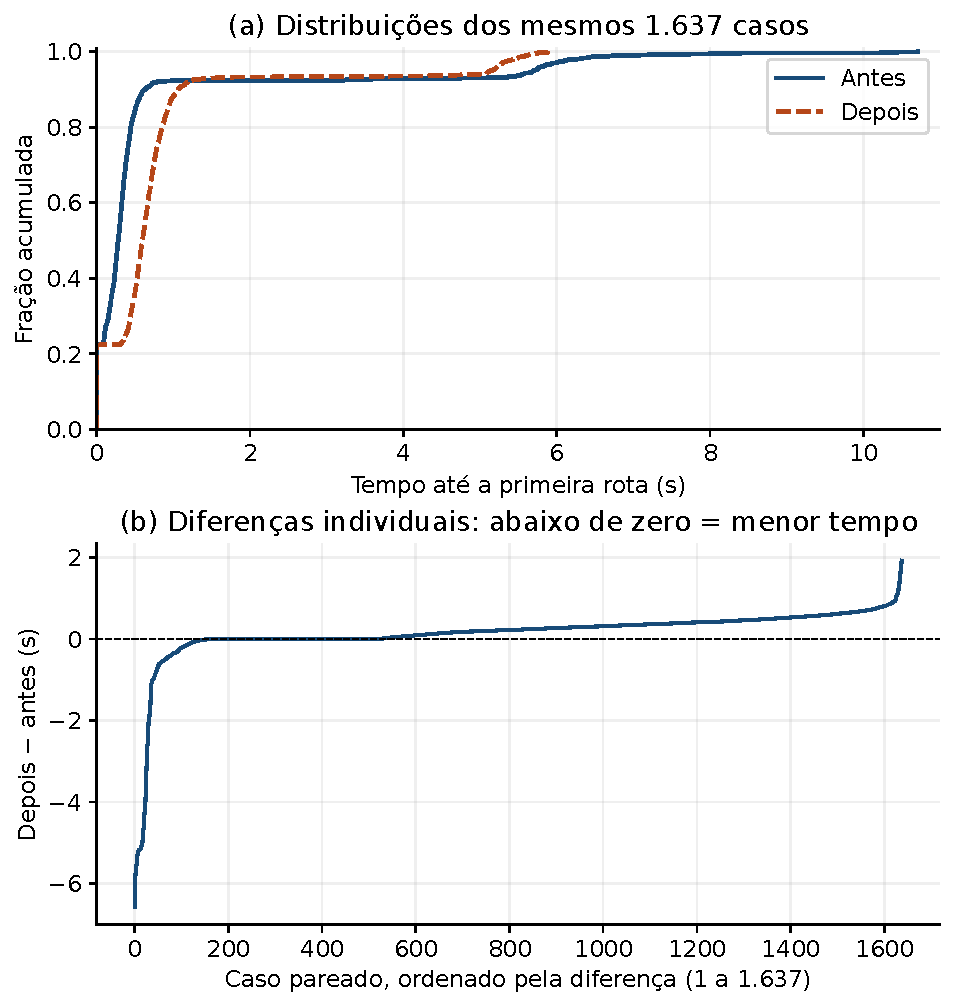
\includegraphics[width=\textwidth]{revisao-tecnico-cientifica-2026-11-02/benchmark-pareado.pdf}
\caption{Distribuições e diferenças das 1.637 medições pareadas até a primeira rota.}\label{fig:benchmark-pareado}
\fonte{CSV individual \nolinkurl{paired-results.csv}, ensaio de 1 nov. 2026; recálculo editorial em 2 nov. Cada diferença é depois menos antes para a mesma consulta; a ordenação não indica sequência temporal.}
\end{figure}
A Figura~\ref{fig:benchmark-pareado} utiliza todos os tempos individuais existentes, sem reconstrução de amostras a partir de médias ou percentis. O P95 segue o instrumento original: elemento ordenado de índice arredondado $0{,}95(n-1)$, com índice inicial zero. Os recortes por horário também mostram heterogeneidade: às 02h, o P95 aumentou de 0,739 para 1,281 s; às 08h, caiu de 5,760 para 5,215 s; às 14h, de 5,766 para 5,204 s. Não foram isolados efeitos de cache, carga, escalonamento ou concorrência; não se atribui causalidade a nenhum deles.

\section{Ampliação metropolitana em Mauá com dados ARTESP}
\label{sec:artesp-maua}
A importação metropolitana acrescentou 25.105 registros de paradas ao cadastro combinado, que passou a conter 47.379 pontos. A base foi ativada no aplicativo público em 2 de novembro de 2026; a consulta ao catálogo confirmou os novos identificadores e a atualização da revisão de cache. A ativação técnica não constitui implantação física de QR Codes nem integração operacional com a gestão municipal. O recorte territorial de Mauá confirmou \textbf{337 paradas ARTESP, 16 linhas ou variantes e 1.491 registros distintos de viagens programadas}, distribuídos pelos três tipos de dia da Tabela~\ref{tab:artesp-maua-dias}. Todas as 337 paradas possuem horários utilizáveis em ao menos um serviço e alternativas estruturais materializadas como origem. Isso não significa atendimento de todas elas em qualquer dia ou horário.

\begin{table}[H]\centering\small
\caption{Oferta programada ARTESP com embarque ou desembarque em Mauá.}\label{tab:artesp-maua-dias}
\begin{tabular}{p{4.7cm}rrr}\hline
Dia de serviço & Paradas & Linhas/variantes & Viagens distintas\\\hline
Dia útil: 03/11/2026 & 337 & 16 & 705\\
Sábado: 07/11/2026 & 324 & 12 & 427\\
Domingo: 08/11/2026 & 324 & 12 & 359\\\hline
\end{tabular}
\fonte{Censo do grupo nos CSV originais ARTESP, versão 20261007, e recorte IBGE 2024; conferência em 2 nov. 2026.}
\end{table}

As 16 entradas de \texttt{routes} são 040, 040EX1, 063, 063EX1, 064, 107, 157, 158, 158BI1, 160, 160EX1, 177, 336, 382, 382EX1 e 403. Extensões e variantes são mantidas como entradas distintas; não se afirma a existência de 16 linhas comerciais independentes. A seleção não se limita aos nomes: seis dessas entradas não mencionam Mauá. As 32.277 passagens por paradas locais presentes no arquivo correspondem a 1.491 viagens distintas, não a 32.277 viagens. Os totais não representam veículos únicos, passageiros ou operações observadas. O mesmo recorte geográfico identificou Capuava (\texttt{18934}), Mauá (\texttt{18935}) e Guapituba (\texttt{18937}), todas na Linha 10--Turquesa, adicionais às 337 paradas metropolitanas.

Foram executadas quatro consultas representativas nos três tipos de dia, com início de planejamento às 08h, no fuso de São Paulo. A Tabela~\ref{tab:artesp-maua-consultas} apresenta uma alternativa identificada em cada cenário e o tempo total estimado desde a consulta, incluindo espera e caminhada. Esses resultados são cálculos com dados reais importados, e não tempos de viagens realizadas em campo.

\begin{table}[H]\centering\small
\caption{Alternativas temporalmente válidas nos horários examinados.}\label{tab:artesp-maua-consultas}
\begin{tabular}{p{8.4cm}rrr}\hline
Cenário e alternativa & Útil & Sábado & Domingo\\\hline
Terminal José Stella (Mauá) ao Terminal Nicolau Delic (São Caetano): ônibus 064, sem baldeação & 130 min & 100 min & 120 min\\[5pt]
Av. Eugênio Negri (Mauá) a Trianon--Masp: 158 e Linha 2, conexão no Sacomã & 145 min & 140 min & 175 min\\[5pt]
R. Oscarito (Mauá) ao Brás: 157 e Linha 10, conexão em Prefeito Saladino & 95,5 min & 105,5 min & 90,5 min\\[5pt]
Estação Mauá a Trianon--Masp: Linha 10 e Linha 2, conexão em Tamanduateí & 68 min & 68 min & 68 min\\\hline
\end{tabular}
\fonte{Leitor de materialização da aplicação, bancos reais, consultas de referência às 08h de 3, 7 e 8 nov. 2026; respostas preservadas na auditoria.}
\end{table}

As conexões envolvendo ônibus têm custo de baldeação 1; a troca interna entre Linha 10 e Linha 2 tem custo $1/3$. A alternativa direta 064 não foi sempre a mais rápida: no dia útil, o mesmo par também retornou 063EX1 e 063, com uma troca e caminhada final, totalizando 98,5 minutos. O leitor reavalia os serviços disponíveis e os horários alcançáveis; não basta existir uma sequência materializada.

No cenário ônibus--trem do dia útil, a resposta calculou embarque no 157 às 08h05, desembarque às 08h43min57s, caminhada de aproximadamente 413 metros até Prefeito Saladino e embarque estimado na Linha 10 às 08h53min57s, com chegada ao Brás às 09h35min27s. O grafo pedestre também contém acesso da parada \texttt{artesp:93038}, na Av. Alberto Soares Sampaio, à estação Capuava: aproximadamente 312 metros e 4,2 minutos. Esse último resultado é a conexão verificada no artefato de caminhadas, não uma inspeção das condições físicas ou da acessibilidade da estação.

Os controles temporais evidenciaram limites. Para Av. Eugênio Negri--Trianon--Masp, às 02h de 3 de novembro, a alternativa 158 e Linha 2 foi calculável, mas exigiu esperar até 04h para o primeiro ônibus; a chegada estimada foi às 06h05min30s. Para o mesmo par, às 08h de 2 de janeiro de 2027, não houve alternativa válida entre os candidatos examinados, após o término do calendário ARTESP. Isso não prova ausência de operação real nessa data. O arquivo cobre 2026 sem exceções de feriados, e a ARTESP informa interpolação linear dos horários nas paradas intermediárias \citep{artespgtfs2026}. A ferrovia mantém o calendário e as estimativas descritos anteriormente. Condições de embarque, acesso, transferência e horizonte de seis horas continuam necessárias.

A materialização combinada, processada com 32 processos, concluiu as etapas de custo 0 e 1, incluindo caminhadas curtas verificadas. As 337 origens metropolitanas locais possuem destinos materializados; não se deduz daí viabilidade temporal para todos os pares. O artefato anterior com custos maiores permanece como fonte complementar para seus identificadores originais. O percentual de 99,666\% e o benchmark de 1 de novembro referem-se ao universo anterior: não são uma taxa de atendimento de Mauá nem uma medição desta expansão. Nas 12 consultas representativas às 08h, o primeiro resultado local variou de 0,295 a 7,830 segundos, com o maior valor observado na primeira carga da rede, sem isolamento causal desse fator; não se trata de benchmark pareado ou latência completa no celular.

Uma consulta adicional pela interface pública, em 2 de novembro às 02h19, retornou 157 e Linha 10 entre R. Oscarito e Brás, com chegada calculada às 06h26. A interface exibiu aviso de busca parcial, preservado junto às capturas: o resultado comprova retorno de uma alternativa, sem assegurar exame de todas as opções ou melhor viagem. Essa captura noturna não representa a consulta programada às 08h da tabela nem demonstra operação de feriado em campo.

A ampliação demonstra um retorno funcional à região que motivou o projeto, por meio de serviços metropolitanos e ferroviários programados. Não incorpora a totalidade da rede municipal de ônibus de Mauá, não fornece previsão ARTESP em tempo real e não comprova cobertura populacional, integração tarifária ou validação com passageiros. A instalação dos QR Codes e a articulação operacional com a gestão municipal permanecem pendentes.

\subsection{Distribuição cadastral e evidência de integração}\label{sec:mapa-artesp}
A Figura~\ref{fig:mapa-artesp} representa as 337 coordenadas existentes no recorte auditado, sem geocodificação ou deslocamento editorial dos pontos. A malha é a municipal IBGE 2024, código 3529401, utilizada na contagem; não foi substituída por um limite simplificado. As estações são símbolos separados e não integram o total das paradas ARTESP. A distribuição é desigual no território e não permite calcular população coberta, acessibilidade física ou disponibilidade operacional.
\begin{figure}[H]\centering
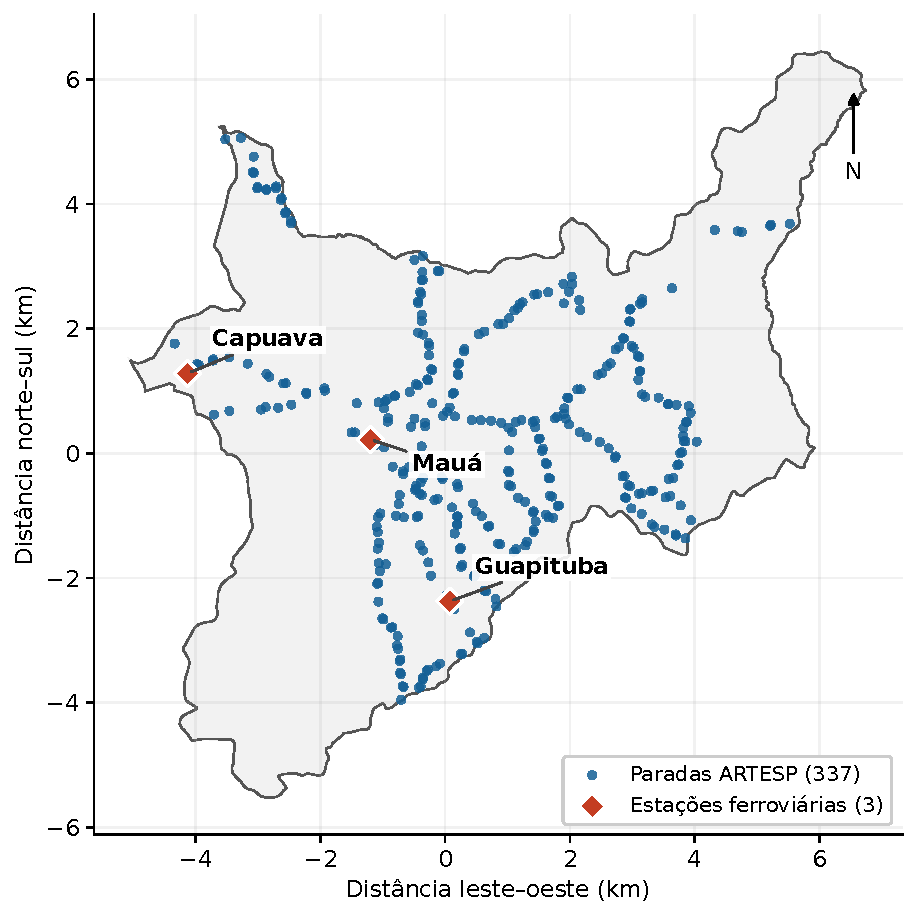
\includegraphics[width=.95\textwidth]{revisao-tecnico-cientifica-2026-11-02/mapa-artesp-maua.pdf}
\caption{Distribuição das paradas ARTESP auditadas e das estações ferroviárias em Mauá.}\label{fig:mapa-artesp}
\fonte{Coordenadas de \nolinkurl{stops.csv} e \nolinkurl{summary.json}; malha \nolinkurl{maua-ibge-2024.geojson}, SIRGAS 2000, auditoria de 2 nov. 2026. Eixos em aproximação métrica local, origem em $(-23{,}67; -46{,}45)$; não representam distância de caminhada.}
\end{figure}
\begin{figure}[H]\centering
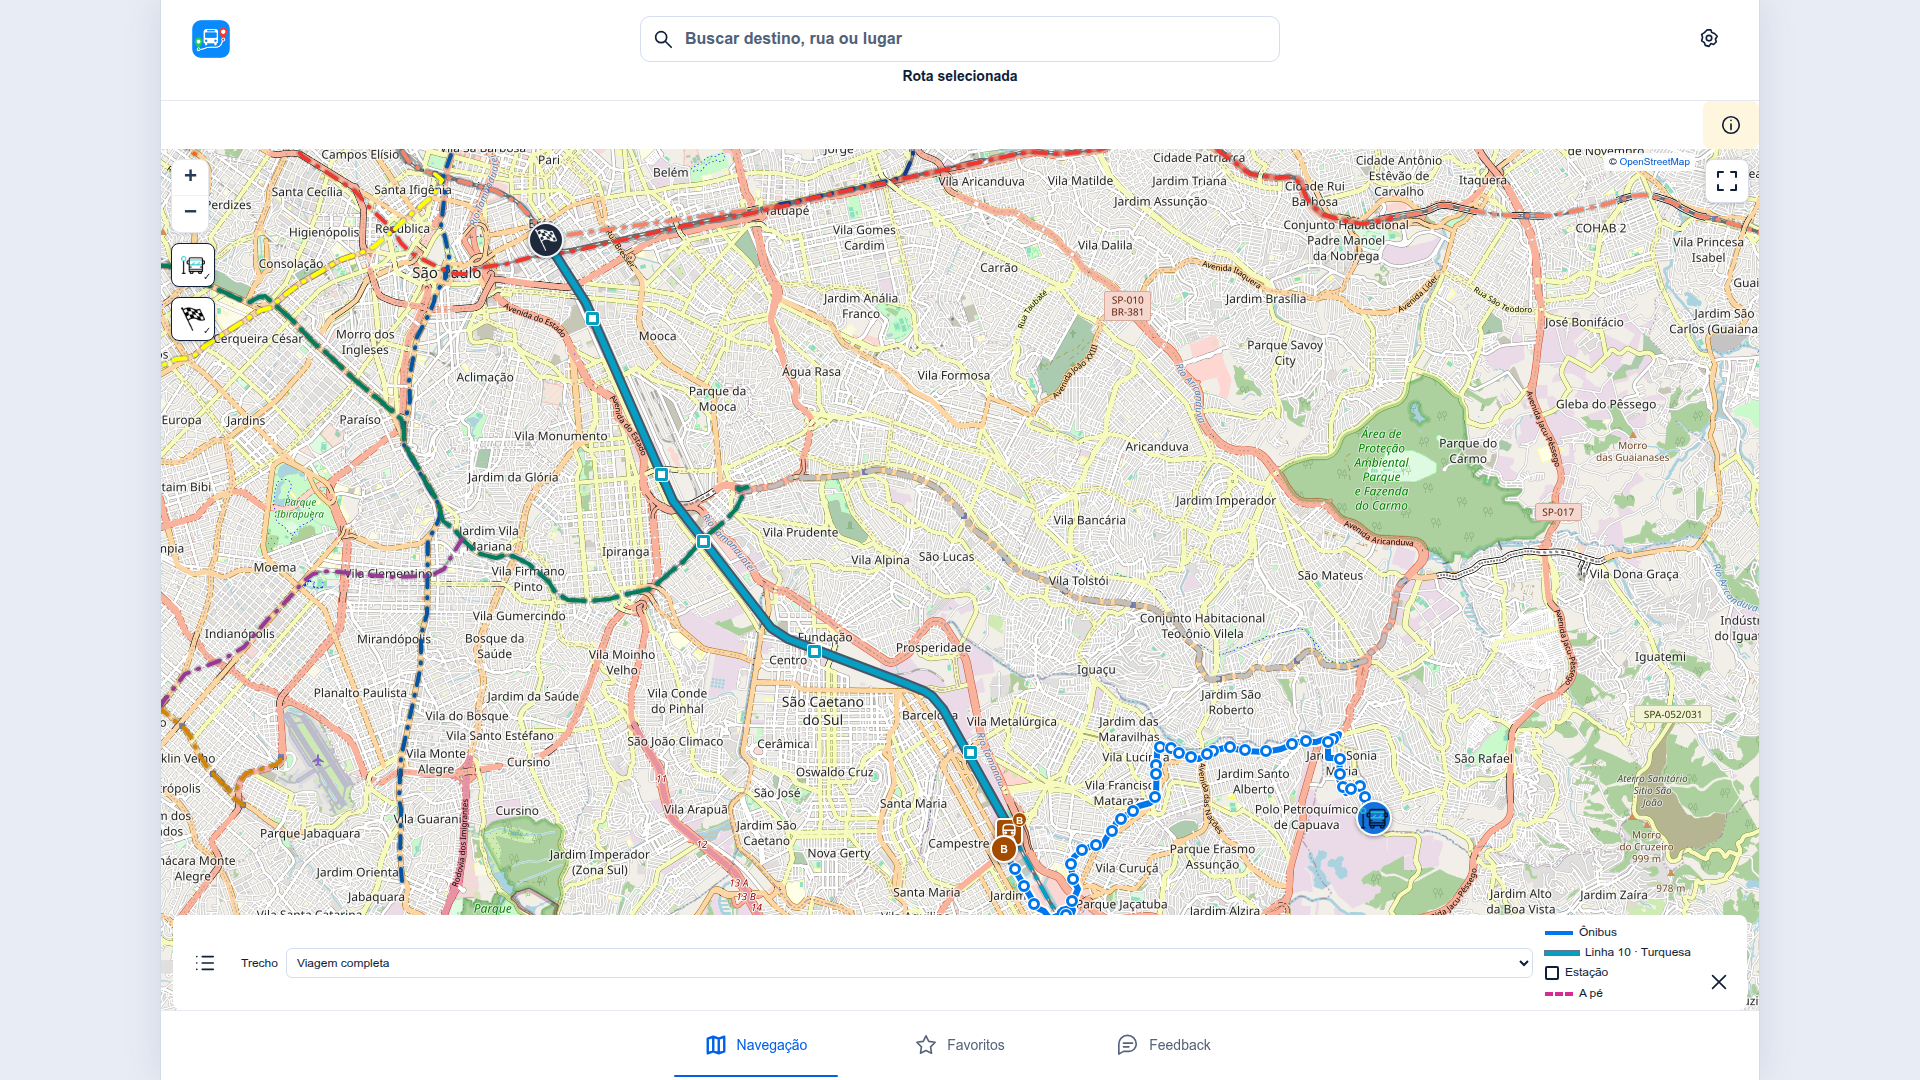
\includegraphics[width=\textwidth,trim=160bp 0 160bp 0,clip]{auditoria-artesp-maua-2026-11-02/captura-maua-bras-mapa.png}
\caption{Consulta Oscarito--Brás com ônibus ARTESP 157 e CPTM Linha 10--Turquesa.}\label{fig:artesp-onibus-trem}
\fonte{Captura da interface em 2 nov. 2026, por volta de 02h19; acervo \nolinkurl{auditoria-artesp-maua-2026-11-02/}. Consulta parcial, com chegada planejada às 06h26; não é uma viagem observada.}
\end{figure}
A Figura~\ref{fig:artesp-onibus-trem} já existia no acervo e demonstra a composição das modalidades na interface. O aviso de busca parcial, visível no painel da Figura~\ref{fig:artesp-consulta-detalhe}, faz parte da evidência e foi mantido. Esta consulta de madrugada não corresponde às consultas das 08h da Tabela~\ref{tab:artesp-maua-consultas}; sua presença não permite substituir resultados, comparar durações entre horários distintos ou afirmar ótimo global. Foram retiradas apenas as margens laterais vazias na diagramação; a imagem original foi preservada. O detalhe da alternativa está na Figura~\ref{fig:artesp-consulta-detalhe}.

\begin{figure}[H]\centering
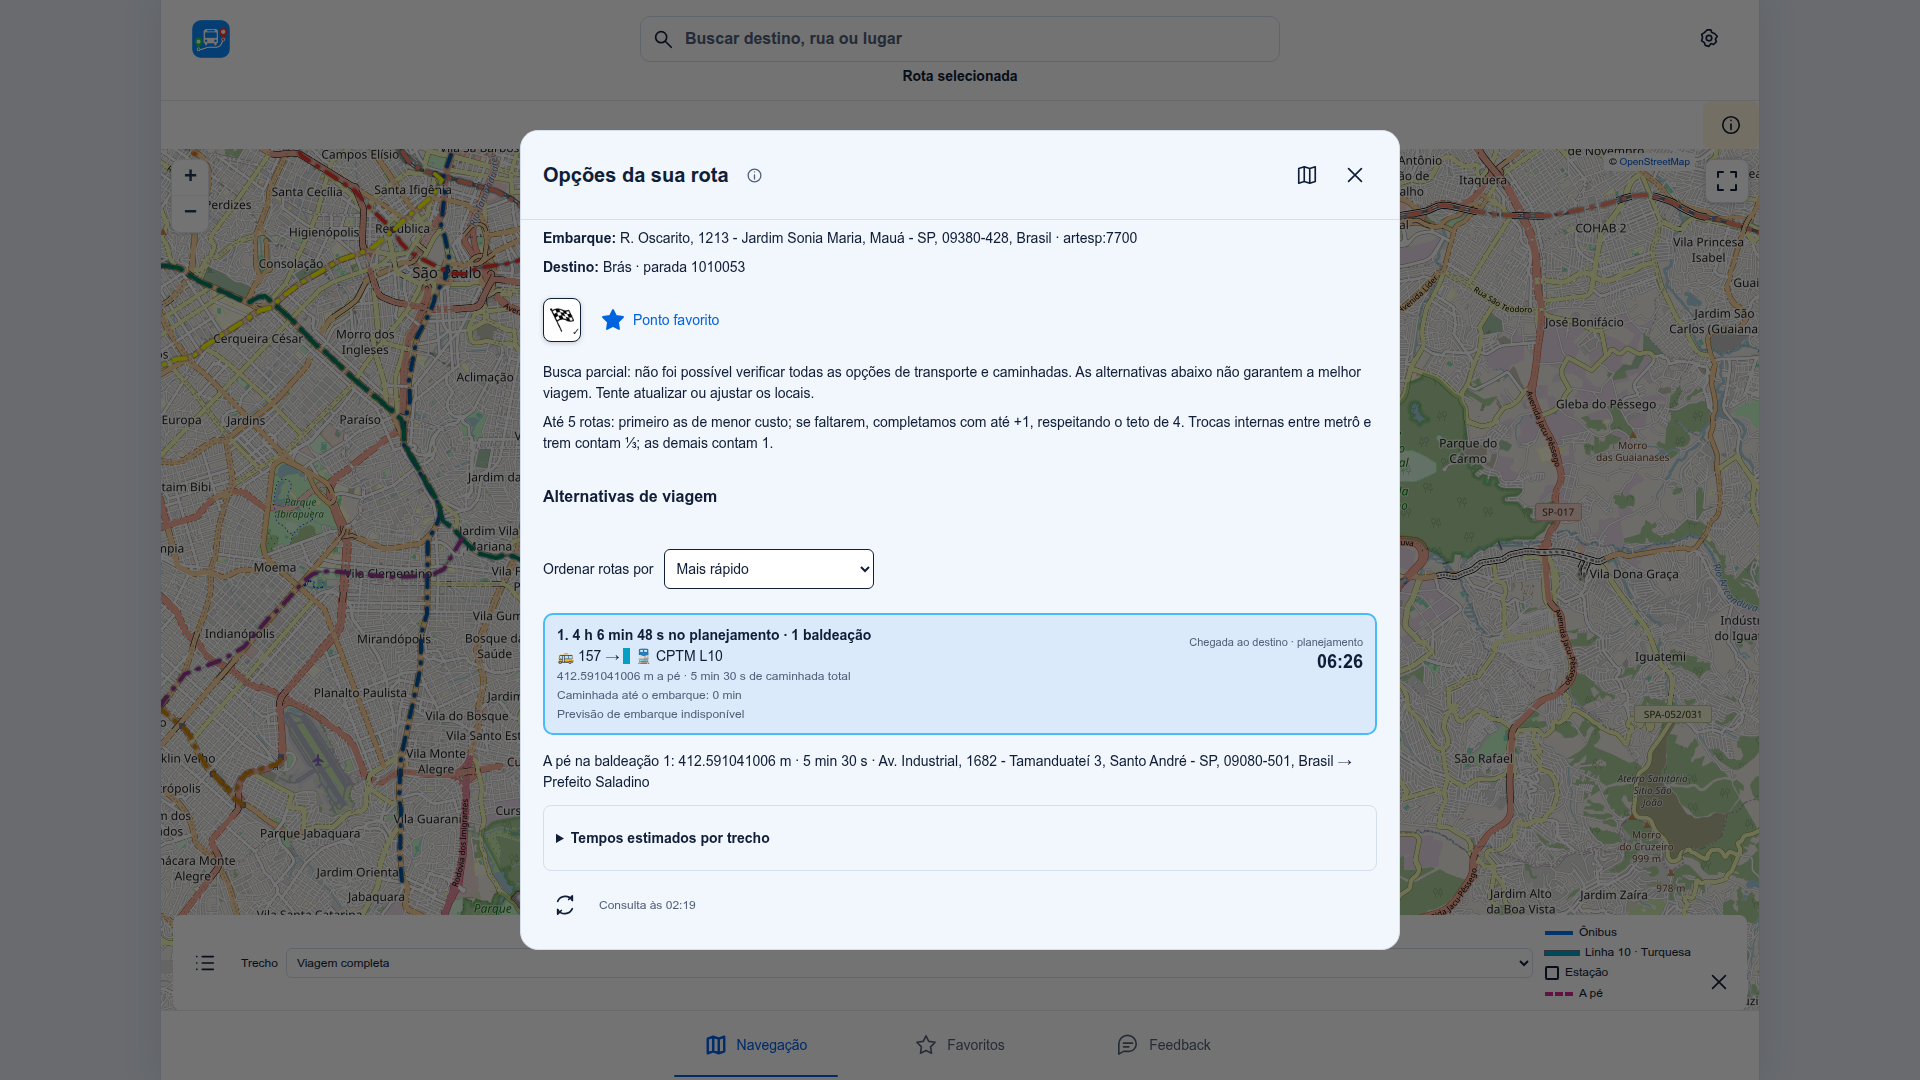
\includegraphics[width=\textwidth,trim=520bp 130bp 520bp 130bp,clip]{auditoria-artesp-maua-2026-11-02/captura-maua-bras-consulta.png}
\caption{Alternativa ônibus--ferrovia e aviso de busca parcial na consulta de madrugada.}\label{fig:artesp-consulta-detalhe}
\fonte{Recorte ampliado do painel da mesma sessão da Figura~\ref{fig:artesp-onibus-trem}, em 2 nov. 2026. Programação e estimativas; não há previsão operacional ARTESP.}
\end{figure}


\section{Avaliação, participação e privacidade}\label{sec:avaliacao-privacidade}
Durante o desenvolvimento, os responsáveis pela implementação utilizaram o PaP em situações de navegação no computador e no celular, identificando dificuldades de interação e apresentação das informações. Essas observações orientaram ajustes na interface e nos fluxos de navegação. Os registros constituem avaliação interna, realizada pelos desenvolvedores também na condição de usuários da aplicação, e não substituem testes com passageiros externos ao grupo.

Um caso dessa avaliação interna ocorreu em 23 de outubro de 2026, quando, durante os testes, os responsáveis pela implementação observaram que o percurso da linha 6L10-41, sentido Messiânica, parecia incorreto no mapa. O trecho contínuo posterior ao embarque encobria parte do tracejado anterior nos locais em que a linha passava novamente pela mesma via. Sem indicação do sentido, o desenho dificultava distinguir uma entrada no bairro seguida de retorno de uma ligação indevida entre ruas. A observação foi registrada no processo de desenvolvimento; não é atribuída a passageiro externo nem ao avaliador técnico.

A conferência da sequência de paradas do GTFS local e da relação de vias da SPTrans apresentada durante a análise identificou o percurso Terminal Varginha, Av. Jaceguava, Av. Prof. Hermann von Ihering, Rua Matilde de Lutis Barbosa, retorno pela Av. Prof. Hermann von Ihering, Av. Jaceguava e Av. do Paiol. Portanto, o retorno por parte das mesmas vias não constituía, isoladamente, evidência de erro de itinerário. A dificuldade de leitura motivou a inclusão de setas e de um pequeno deslocamento lateral dos traços conforme o sentido de circulação. Esse afastamento é apenas gráfico, em pixels: não altera as coordenadas cadastradas, as paradas ou o cálculo das viagens, e não representa a posição exata de uma faixa de trânsito.

\begin{figure}[H]\centering
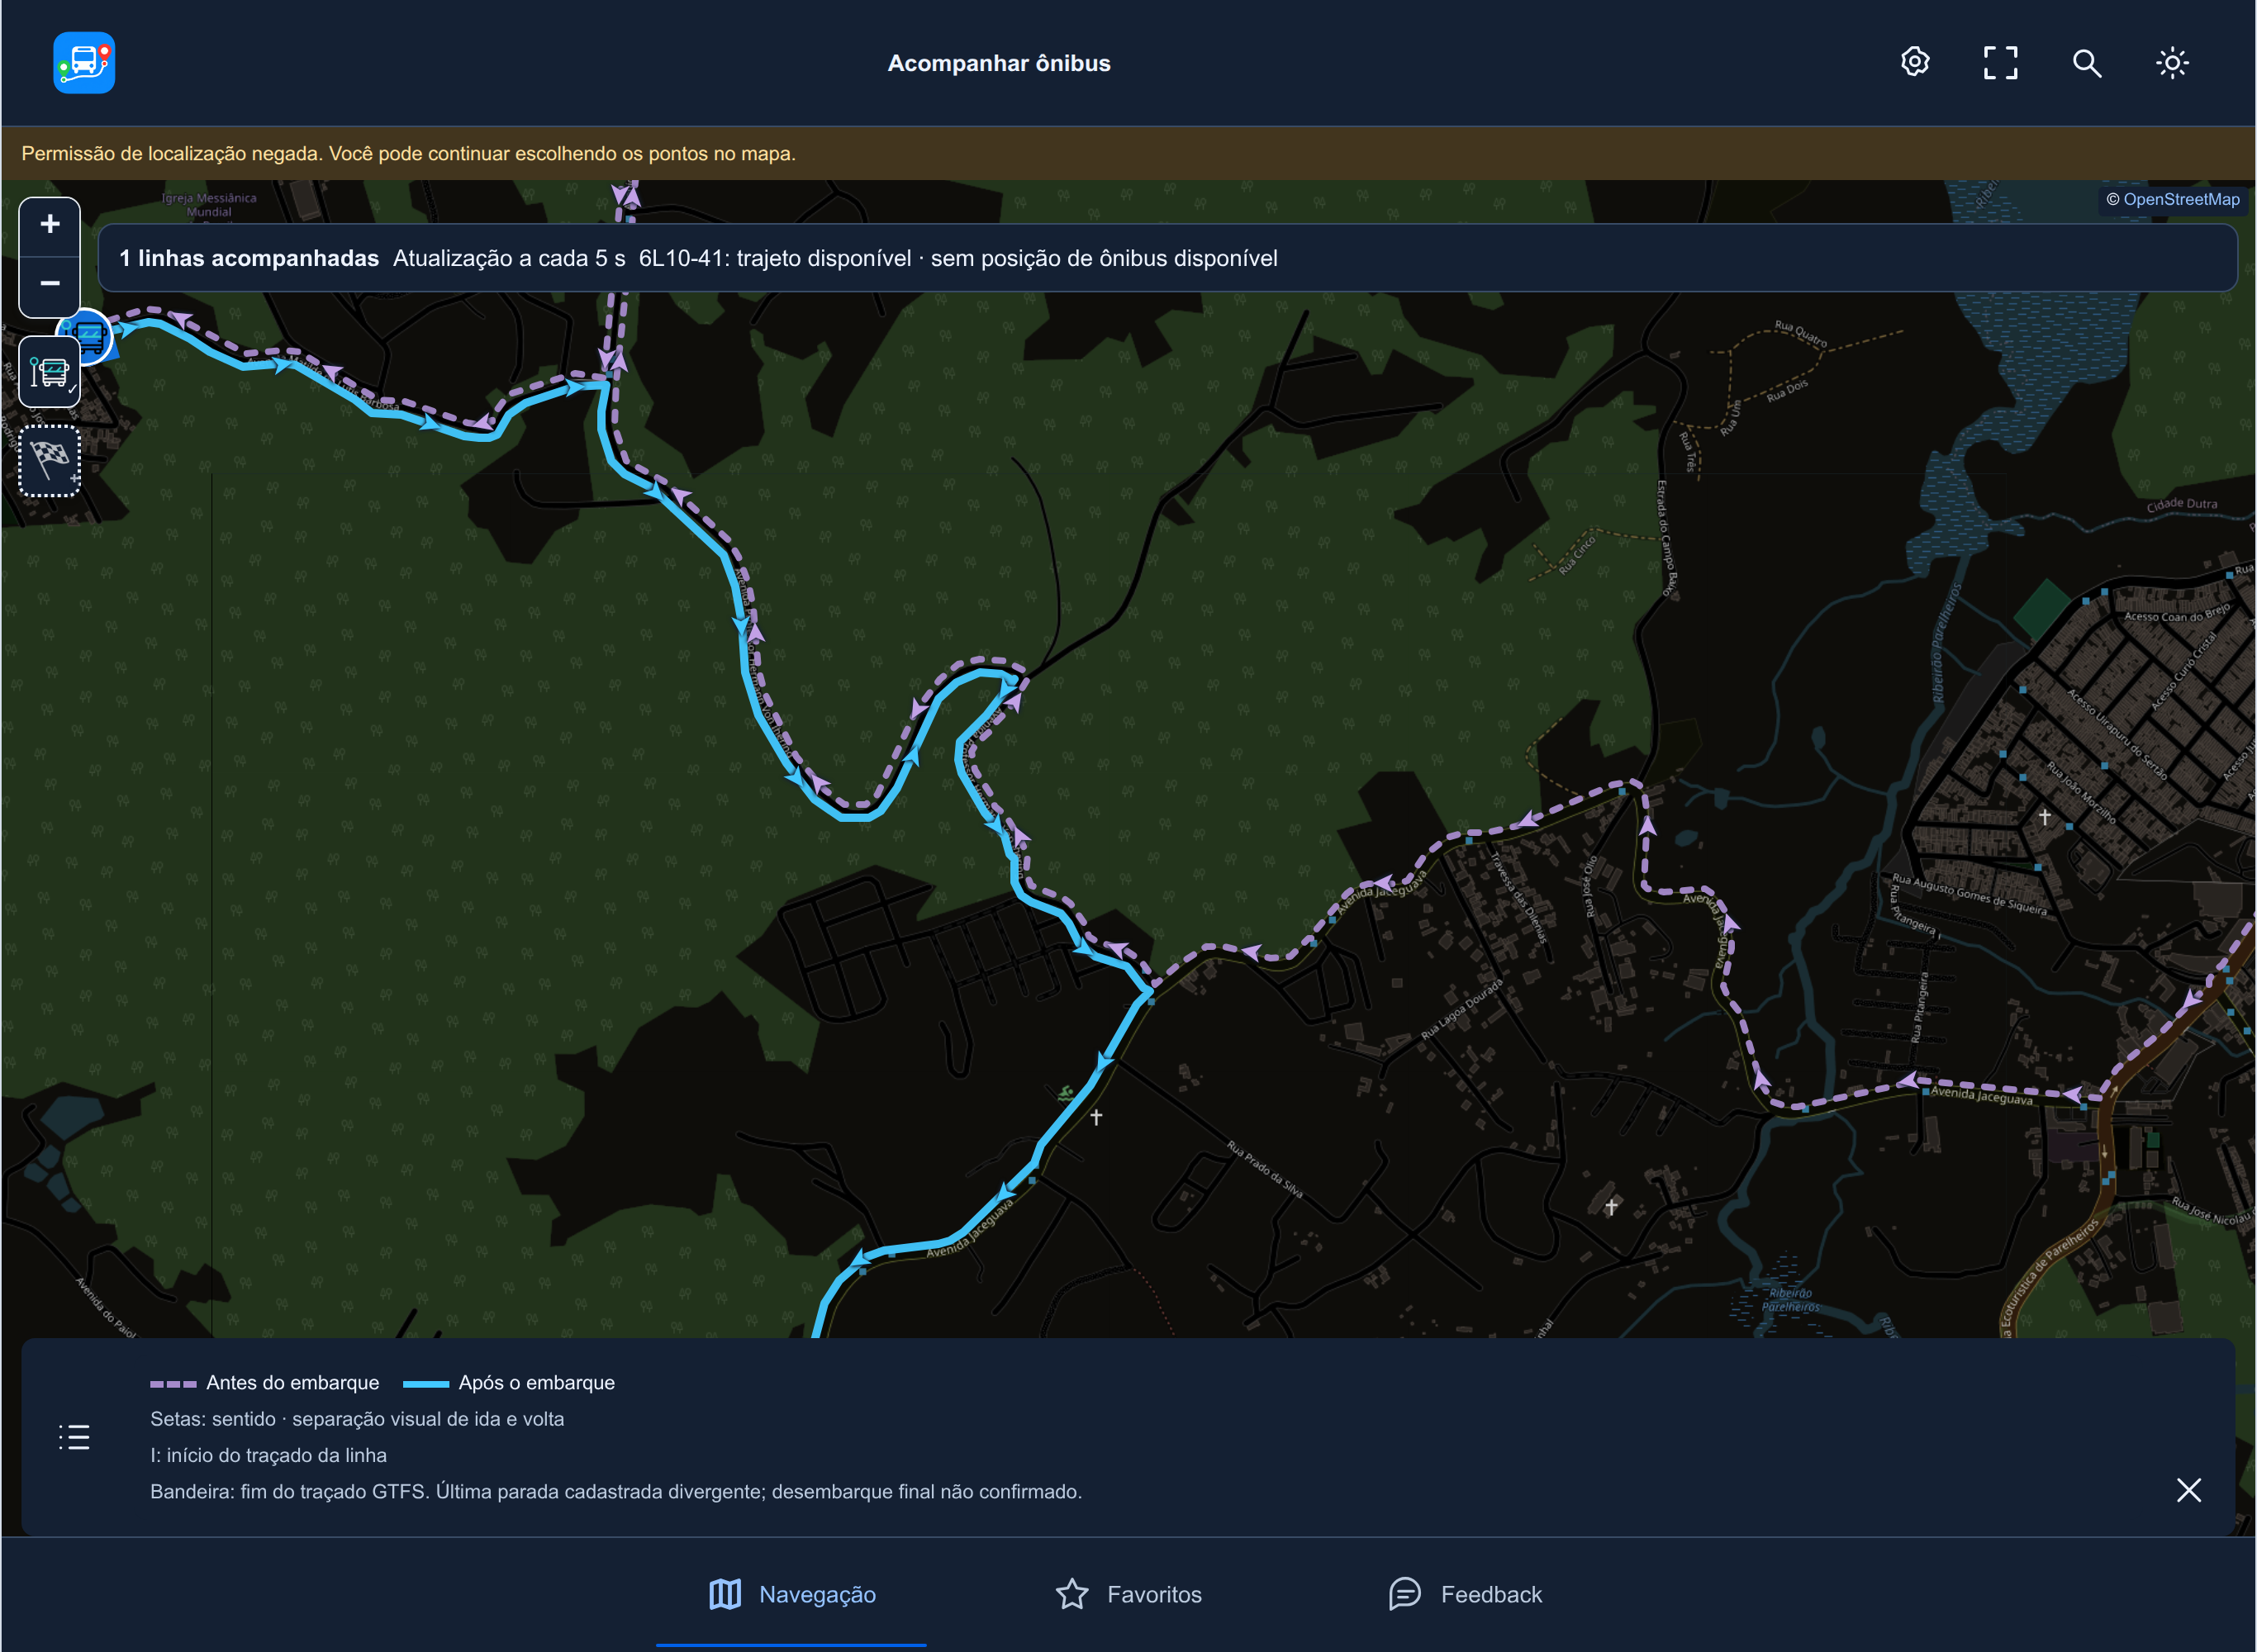
\includegraphics[width=\textwidth,height=0.56\textheight,keepaspectratio]{capturas/2026-10-25-sem-aviso/linha-6L10-detalhe.png}
\caption{Detalhe da linha 6L10-41 após a correção: setas e separação visual das passagens em sentidos opostos.}\label{fig:rotas-sobrepostas}
\fonte{Captura real da aplicação, ampliada pelo controle de zoom do mapa, revisão 85417bc com recaptura após ajuste local da interface, 25 out. 2026.}
\end{figure}

O lilás tracejado identifica a parte anterior ao embarque selecionado e o azul contínuo identifica a parte posterior. Esses estilos se referem ao ponto escolhido, não ao histórico de deslocamento de um veículo. O início é indicado por ``I'', e o botão de retorno à lista permanece à esquerda. A seleção do traçado completo também foi disponibilizada quando não há previsão ou posição de ônibus; ausência de informação operacional não impede consultar o itinerário cadastrado.

Foi identificada, separadamente, uma divergência entre a última parada cadastrada, Av. do Paiol, 1413, e o término da geometria da viagem \texttt{6L10-41-1}. Em vez de cortar o percurso ou criar uma parada não confirmada, a aplicação preserva o traçado e apresenta a bandeira como ``fim do traçado GTFS'', acompanhada da ressalva de que o desembarque final não está confirmado. Essa sinalização explicita a incerteza; não corrige nem valida operacionalmente a fonte de dados.

A verificação da mudança de direção visual incluiu testes automatizados com coordenadas artificiais, cobrindo percursos opostos e pontos repetidos, além de regressões em navegador para linhas com e sem veículos, acompanhamento individual e divergência do ponto final. Na execução registrada durante a implementação, passaram 49 testes unitários de frontend e quatro testes de navegador. Esses resultados verificam comportamento de software; não demonstram melhora mensurada de usabilidade. As capturas desta revisão utilizam dados reais e documentam o estado posterior à correção, sem reconstrução sintética de uma tela anterior.



Para complementar a observação interna, na versão atualizada em 23 de outubro de 2026, a coleta de navegação depende da participação voluntária e está implementada para investigar dificuldades de interação e falhas. Os registros são agrupados por sessão em banco separado do cadastro de transporte. Incluem a reprodução visual da interface e do mapa, movimentos e toques, rolagem e ações, textos de busca, origem e destino, localização quando autorizada no navegador, estado dos favoritos e das rotas, parâmetros e respostas das consultas, erros e metadados do dispositivo. A reprodução visual permite reconstituir a interface; os eventos e resultados de consultas ajudam a localizar falhas; os metadados permitem relacioná-las ao navegador e às dimensões de tela. Comentários enviados voluntariamente pelo botão de feedback são armazenados separadamente e podem ser vinculados à sessão quando a pesquisa está ativa; o envio também é permitido sem gravação de navegação. Um identificador de sessão não torna anônimos os locais e textos registrados.

O aviso da Figura~\ref{fig:print-02-informacoes} permite ``Contribuir com a pesquisa'' ou ``Continuar sem contribuir''. A recusa mantém as funções de transporte disponíveis, sem iniciar sessão de telemetria ou reprodução visual. Falhas de gravação não devem bloquear a consulta. A escolha, sua versão e data são persistidas no navegador, sem prazo arbitrário de expiração; alterações relevantes no aviso exigem nova decisão. Ausência ou falha do armazenamento não equivale a consentimento. Em Configurações, o participante pode consultar ou alterar sua decisão, interromper a captura e solicitar exclusão. A interrupção descarta eventos não enviados e impede novos envios, mas não exclui automaticamente dados já recebidos. Consultas operacionais de transporte e logs do servidor são distintos da participação na pesquisa.

\begin{figure}[H]\centering
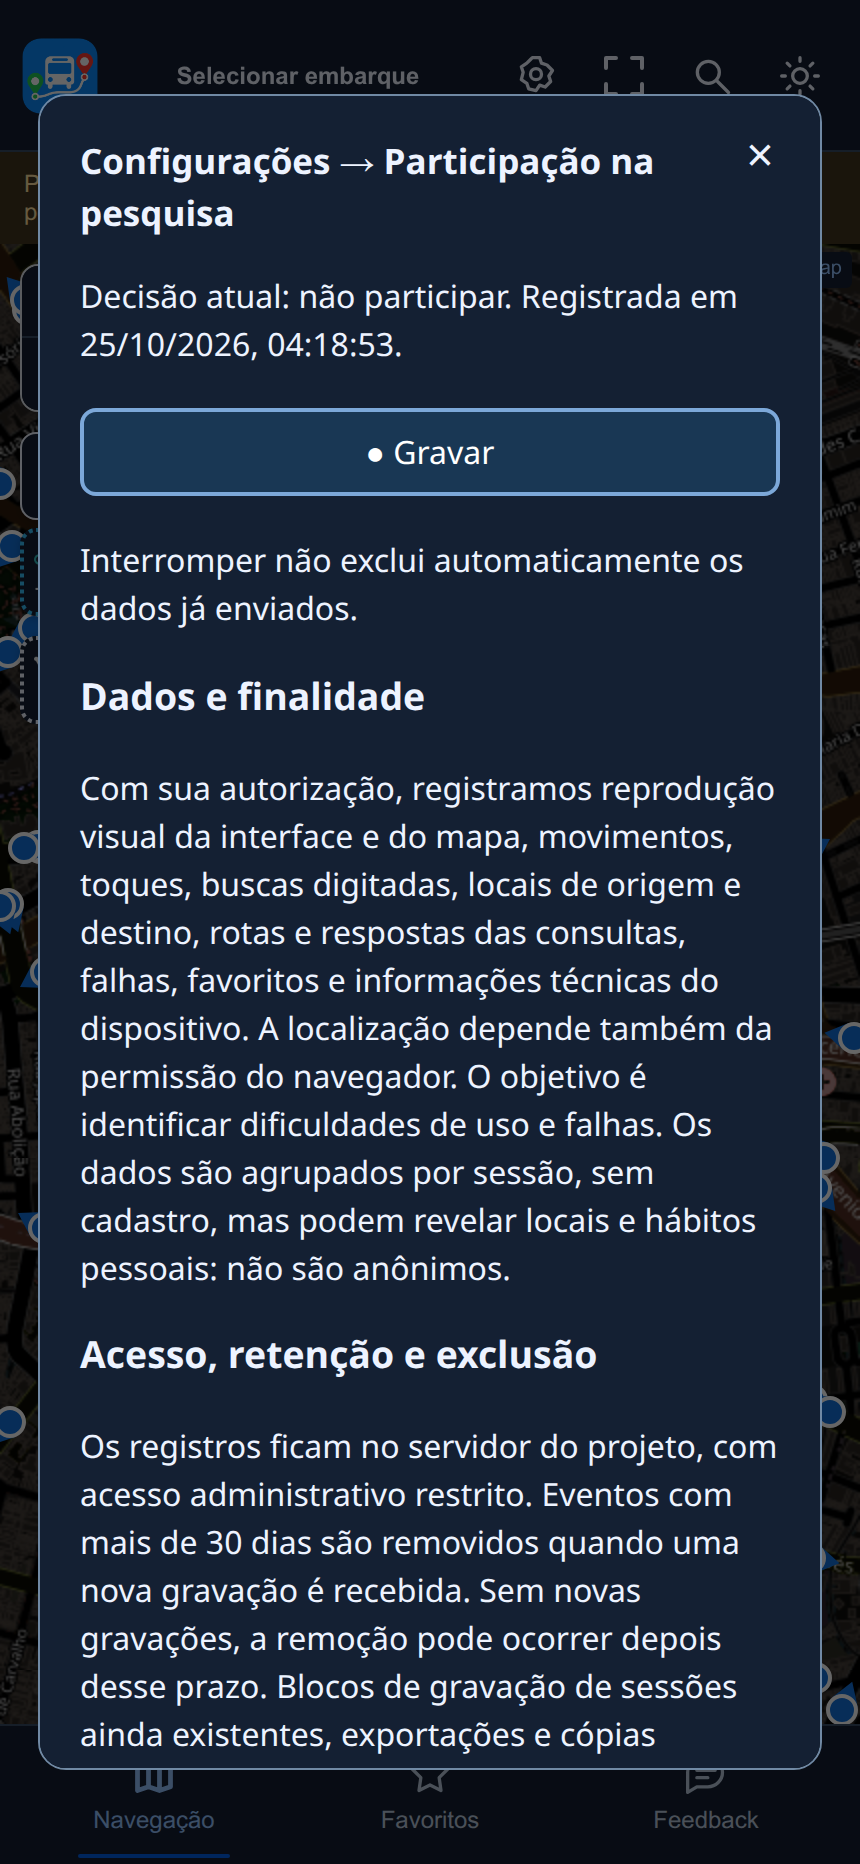
\includegraphics[width=0.43\textwidth,height=0.55\textheight,keepaspectratio]{capturas/2026-10-25-sem-aviso/pesquisa-configuracoes.png}\hfill
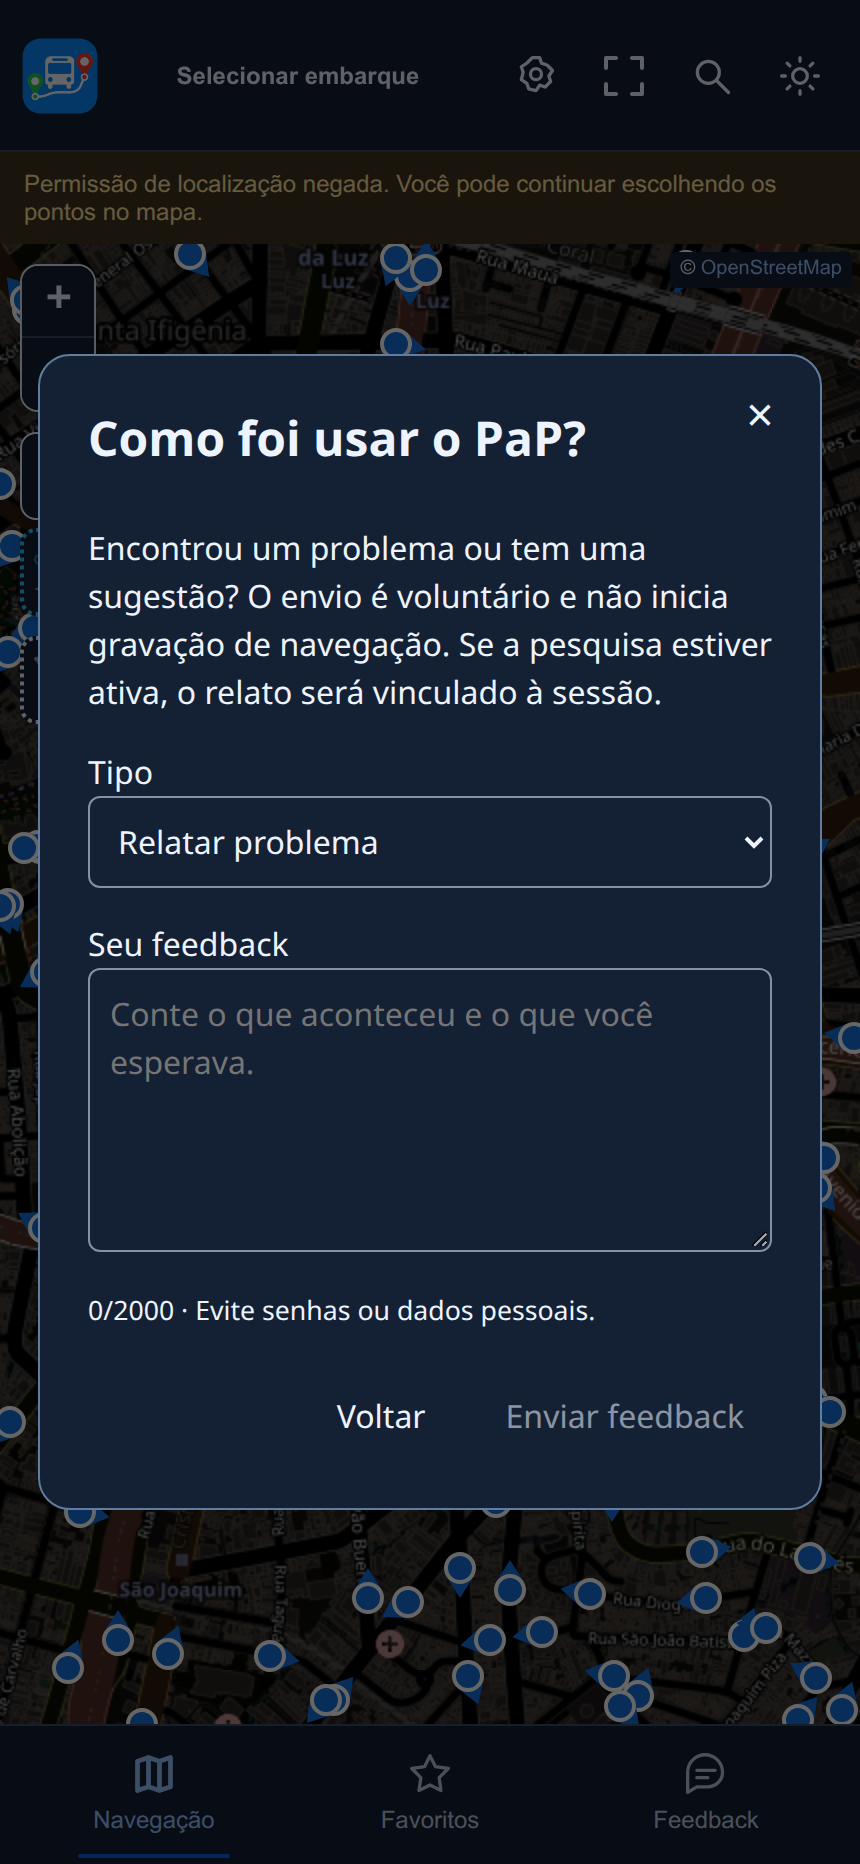
\includegraphics[width=0.43\textwidth,height=0.55\textheight,keepaspectratio]{capturas/2026-10-25-sem-aviso/feedback.png}
\caption{Decisão de não participar nas configurações e formulário de feedback voluntário.}\label{fig:pesquisa-voluntaria}
\fonte{Capturas reais da aplicação em viewport móvel, revisão 85417bc com recaptura após ajuste local da interface, 25 out. 2026.}
\end{figure}
As configurações possuem conteúdo rolável: a captura mostra a parte inicial, não a integralidade das informações. O formulário de feedback foi aberto sem enviar mensagem. Essas telas documentam a separação entre consulta ao transporte, pesquisa e manifestação voluntária.

O prazo de 30 dias informado na interface corresponde ao critério de remoção dos eventos antigos, contado a partir do recebimento no servidor. A limpeza é executada no processamento de um lote de telemetria validado, não por uma tarefa periódica independente. Sem novas gravações, a remoção pode ocorrer depois desse prazo. Os blocos comprimidos reutilizados dentro de uma sessão são eliminados quando ela deixa de possuir eventos. Enquanto restar algum evento, blocos associados a registros já expirados podem permanecer. Arquivos exportados não são abrangidos automaticamente pela limpeza por idade. Assim, a implementação não assegura a eliminação de todas as cópias em até 30 dias. O acesso pela aplicação exige autenticação administrativa, e a configuração de acesso público bloqueia a administração. A exclusão manual de uma sessão, com confirmação, remove seus eventos e blocos associados e tenta remover o diretório de exportações em cache. Falhas nessa remoção de arquivos são ignoradas pelo código, de modo que o retorno da operação não garante a eliminação de todas as cópias. Cópias previamente baixadas precisam de tratamento próprio. A exclusão lógica no SQLite também não equivale a apagamento físico garantido nem reduz necessariamente o tamanho do arquivo. A interface permite solicitar exclusão, sujeita à análise da equipe; o protocolo de recebimento não significa eliminação imediata. Relatos voluntários e solicitações são armazenados separadamente, não são removidos pela exclusão da sessão e não possuem limpeza automática por prazo nesta versão. Sua exclusão administrativa é uma ação distinta; marcar uma solicitação como resolvida não elimina seus dados nem executa automaticamente a exclusão dos registros de navegação.

O protótipo registra eventos de navegação para diagnóstico de usabilidade, incluindo origem e destino, mas não consolida esses registros em indicadores agregados de demanda. Essa finalidade analítica permanece uma possibilidade futura; pesquisas populacionais estão fora da entrega atual. Sua utilidade deverá ser discutida com o interlocutor e responsáveis pelo planejamento, definindo quais decisões os indicadores poderiam apoiar e como confrontá-los com levantamentos operacionais. Uma eventual confirmação voluntária de embarque ou desembarque seria um dado adicional autodeclarado, sujeito a validação própria.

A interlocução técnica externa foi ampliada com Thiago Almeida Amorim, da Alameda Solutions, conforme o registro a seguir. Permanece necessária a avaliação específica com passageiros, documentando sua relação com o transporte local e os critérios de seleção. A ausência de resposta aos contatos recentes com o interlocutor inicial constitui uma limitação de continuidade, sem invalidar suas contribuições à definição do problema. O grupo poderá revisar a experiência de uso e aprimorar diretamente a aplicação funcional conforme as observações recebidas. O Figma permanece como registro histórico da prototipação. A avaliação de compreensão com passageiros ainda será realizada, com planejamento e registro próprios. As capturas da aplicação avaliada deverão identificar revisão e cenário; as alterações decorrentes do feedback serão documentadas. A avaliação deve verificar especialmente se o usuário reconhece a natureza das informações apresentadas, distinguindo dados cadastrais, coordenadas aproximadas, horários programados, previsões operacionais e, quando aplicável ao cenário histórico de Mauá, informações simuladas.

Para incorporar a rede municipal de ônibus de Mauá, ainda será necessário obter e confrontar seu cadastro operacional e revisar os registros sem coordenadas e as estimativas do levantamento histórico. Essa pendência não bloqueia a cobertura metropolitana programada já habilitada com ARTESP e ferrovia. Cobertura, duplicidades entre fontes, lado da via, acessibilidade, vigência e sentido exigem conferência antes de ampliar a base municipal. A instalação física de QR Codes e a articulação com a gestão local permanecem etapas distintas da ativação técnica do aplicativo.

\begingroup\setlength{\parskip}{8pt}
A interlocução externa foi realizada com Thiago Almeida Amorim, da Alameda Solutions, CNPJ 60.184.290/0001-00, por intermédio da integrante Nathalia Almeida Amorim. Essa identificação substitui a designação provisória utilizada nos registros preparatórios. O escopo compreendeu o aplicativo Ponto a Ponto e o relatório técnico, excluindo ferramentas e requisitos de produção audiovisual.

Em 21 de outubro de 2026, Thiago apresentou o primeiro feedback sobre as modificações realizadas até aquela data. A análise do relatório contemplou a arquitetura Django/Python, React e SQLite, a integração GTFS e Olho Vivo da SPTrans e a descrição do planejador híbrido, com composição bidirecional, materialização seletiva e busca por rodadas como alternativa. Em 25 de outubro de 2026, enviou uma atualização abrangendo as modificações posteriores do aplicativo e do relatório. As sugestões tiveram origem na revisão interna do grupo e nas navegações de usuários relatadas pelo grupo; a avaliação dos resultados foi atribuída a Thiago.

Segundo a confirmação fornecida pelo grupo, o avaliador examinou os 26 itens consolidados no Apêndice~\ref{ap:feedback-alameda}, considerou as melhorias avaliadas devidamente implementadas e reconheceu contribuição positiva para a qualidade da experiência de uso. A conclusão qualitativa de IHC abrange clareza das informações, visibilidade do estado, controle da navegação, prevenção de erros e redução de esforço. No relatório, abrange clareza dos modelos, coerência com o aplicativo e distinção entre evidências e limitações. Essa apreciação não corresponde a medição quantitativa de usabilidade nem comprova execução independente dos testes automatizados pelo avaliador.

A atualização de 25 de outubro adota como referências o aplicativo na revisão \texttt{85417bc}, branch \texttt{feat/busca-bidirecional}, e o relatório na revisão \texttt{c18556c}, branch \texttt{relatorio}. O commit correspondente ao primeiro feedback de 21 de outubro não está identificado no acervo consultado; as revisões posteriores não são atribuídas retroativamente àquela data. A presente consolidação documental é posterior ao relatório de referência e incorpora a identificação definitiva e a comunicação recebida.

O grupo informou que o conteúdo e o alcance da avaliação foram confirmados e que o documento foi assinado. Em 26 de outubro de 2026, disponibilizou o arquivo reproduzido no Anexo~\ref{an:parecer-thiago}, com assinatura visível na primeira página, identificação do cargo de sócio-administrador e indicação de São Paulo--SP e 25 de outubro de 2026 como local e data da assinatura. O documento registra autorização para divulgação identificada e confirmação das versões examinadas. Os campos finais de alcance, conclusão, data e visto foram preenchidos conforme autorização escrita do avaliador disponibilizada pelo grupo em 26 de outubro; a assinatura existente foi reutilizada no visto, com a data de 25/10/26 solicitada. O arquivo recebido originalmente e a autorização foram preservados. As versões preparatórias permanecem separadas do documento recebido.

A avaliação externa complementa a interlocução inicial com o transporte público de Mauá e não substitui uma avaliação específica de compreensão com passageiros. O histórico, a resposta aos ajustes e os limites documentais constam do Apêndice~\ref{ap:feedback-alameda}.\par\endgroup

Além da apreciação profissional, o grupo convidou usuários reais a explorar o PaP e avaliar o resultado. As navegações e os comentários disponíveis entre 19 e 26 de outubro de 2026 constituem uma avaliação exploratória com usuários convidados, sem roteiro padronizado de tarefas ou caracterização suficiente para representar passageiros em uso cotidiano. A análise documental abrangeu 36 sessões e 50.989 eventos do acervo local; esses totais incluem duas sessões identificadas como automatizadas, excluídas da interpretação do comportamento humano. Sessões não equivalem a pessoas distintas, e não foi estabelecido um número de participantes únicos. Foram considerados estados da aplicação, ações, respostas de serviços, metadados de dispositivo e feedbacks, sem tomar a repetição de ações como prova de dificuldade.

Em 19 de outubro, às 17h16--17h17, em celular Android com Chrome, uma sessão manteve embarque e destino após defini-los e alternou entre painel e mapa, consultando alternativas associadas às linhas 107T-10, 7181-10 e 908T-10. Esse comportamento é compatível com exploração e comparação de rotas, sem evidência de reformulação da busca naquele trecho. Em 25 de outubro, entre 13h24 e 13h36, em Android com Firefox, outra sessão reformulou endereços, mudou embarque e destino e selecionou uma alternativa a pé antes de cancelar. Essas ações podem integrar a avaliação deliberada do protótipo. Uma chamada de planejamento registrou aproximadamente 33 segundos, mas já havia informação de viagem antes de seu término; esse valor não corresponde necessariamente ao tempo até a primeira resposta utilizável.

Os relatos acrescentaram a percepção dos avaliadores. Uma captura de 25 de outubro, às 13h31, em interface móvel, registra pedido de maior clareza nos controles de embarque e destino e falha ao salvar o feedback. Em mensagem editada às 13h40, sem dispositivo identificado, um usuário informou que a navegação fluiu melhor após compreender o funcionamento, solicitou maior destaque para os controles e relatou diferença entre escolher uma parada no Terminal Sacomã e pesquisar o endereço. Essas mensagens não possuem vínculo inequívoco com um identificador de sessão. Às 13h47min49s, um feedback efetivamente salvo, vinculado a uma sessão em Android com Firefox, elogiou a integração do Olho Vivo à rota e a ausência de interrupções por anúncios. Os horários estão no fuso de São Paulo; o horário de edição da mensagem não identifica o momento exato da tarefa.

Em 26 de outubro, às 13h17--13h18, uma sessão em Android com Chrome avançou da consulta de parada ao mapa de uma viagem. A inspeção identificou a mesma parada como origem e destino, de modo que a abertura do percurso comprova exploração da funcionalidade, não atendimento a uma necessidade real de deslocamento. Em conjunto, os registros sustentam a realização de avaliação exploratória por usuários reais convidados e o reconhecimento de benefícios e oportunidades de melhoria. Não permitem estimar taxa de sucesso, satisfação geral ou fluidez cotidiana dos passageiros. Sugestões, problemas técnicos e exploração são evidências distintas; comentários alheios ao produto foram desconsiderados.

Em 29 de outubro de 2026, o grupo conferiu a implementação e os registros de testes das mudanças relacionadas aos relatos de 25 de outubro. A Tabela~\ref{tab:feedback-ajustes} distingue correção técnica, sugestão parcialmente atendida e benefício já existente. Trata-se de uma etapa posterior ao parecer de Thiago; não constitui nova avaliação pelo profissional nem reavaliação com os usuários convidados. Os horários identificam as fontes, não participantes independentes.

\begingroup\small\SingleSpacing\setlength{\parskip}{0pt}\setlength{\LTcapwidth}{\textwidth}
\begin{longtable}{>{\raggedright\arraybackslash}p{3.3cm}>{\raggedright\arraybackslash}p{6.1cm}>{\raggedright\arraybackslash}p{5.2cm}}
\caption{Encaminhamento dos feedbacks e estado da verificação em 29 de outubro.}\label{tab:feedback-ajustes}\\\hline
Origem e observação & Alteração ou benefício preservado & Verificação e limite\\\hline\noalign{\vskip 4pt}\endfirsthead
\hline Origem e observação & Alteração ou benefício preservado & Verificação e limite\\\hline\noalign{\vskip 4pt}\endhead
\hline
\multicolumn{3}{p{\dimexpr\linewidth-2\tabcolsep\relax}}{\footnotesize Fonte: Elaboração do grupo a partir dos relatos de 25/10 e das verificações técnicas de 28 e 29/10/2026. Textos sintetizados, sem atribuição de novas opiniões aos avaliadores.}\\
\endlastfoot
13h31 e 13h40: maior clareza e dois campos para embarque e destino. & Os controles exibem rótulos e o local ou estado da seleção. A troca do papel da busca limpa a confirmação anterior. & Comportamento e disposição em telas móveis e desktop conferidos. São dois controles, não dois campos simultâneos de digitação; compreensão ainda não reavaliada.\\ \noalign{\vskip 8pt}
13h40: melhorar a busca. Replay examinado: sugestão de outra rua. & Na consulta com número e tipo explícito de via, a sugestão precisa corresponder ao nome normalizado da rua. & Caso reconstruído rejeita a rua divergente e aceita a correta. Não demonstra precisão geral do geocodificador nem resolve toda ambiguidade de endereço.\\ \noalign{\vskip 8pt}
13h40: parada e endereço produziram resultados distintos no Sacomã. & Seleção de todas as paradas de ônibus em até 200 m; sem nenhuma, até três mais próximas, preservando o limite de caminhada de 1 km. & Na coordenada examinada, 24 registros candidatos em vez de três. Percursos a pé e horários continuam sujeitos a validação; resolução do episódio histórico não comprovada.\\ \noalign{\vskip 8pt}
13h31: falha ao salvar feedback. & Envio externo liberado; falhas preservam nota e texto ao fechar e reabrir o formulário. Nova tentativa conserva o identificador se o conteúdo não mudar. & Persistência com e sem pesquisa, erros e retentativas verificados. O responsável atribuiu o incidente ao bloqueio de acesso externo; falta vínculo inequívoco com a requisição histórica.\\ \noalign{\vskip 8pt}
Replay do Sacomã: caminhada apresentada com busca incompleta. & Aviso de busca parcial também aparece quando há uma alternativa a pé. & Estado reproduzido no navegador. A advertência informa a limitação; não comprova recuperação de uma alternativa de ônibus.\\ \noalign{\vskip 8pt}
13h40 e 13h47min49s: Olho Vivo integrado; 13h47min49s: ausência de anúncios. & Benefícios existentes preservados, sem atribuir sua criação às correções posteriores. & Integração conferida com respostas simuladas e interface inspecionada. Não assegura disponibilidade permanente da fonte operacional.\\ \noalign{\vskip 4pt}
\end{longtable}
\endgroup

A reconstrução do replay não mostrou um confronto controlado entre parada e endereço: as consultas examinadas utilizaram origens diferentes e plataformas 4 e 5. Seu vínculo com a mensagem das 13h40 não é inequívoco. A ampliação dos acessos responde à concentração de paradas próximas, mas não estabelece a causa única do relato. Os 24 candidatos são registros do catálogo, não necessariamente plataformas físicas distintas. A regra completa de acesso está descrita na Seção~\ref{sec:historico-arquitetura}.

Como complemento definido pelo grupo, o formulário passou a aceitar uma avaliação opcional de uma a cinco estrelas, sem nota pré-selecionada. Com nota, o comentário é opcional; sem nota, permanece necessário. O envio não inicia gravação de navegação. Os registros anteriores continuam sem nota: a nova funcionalidade não produz uma série retrospectiva nem uma medida de satisfação já coletada. O rascunho é preservado ao reabrir o formulário, mas não ao recarregar a página.

A conferência utilizou testes com bases temporárias e respostas controladas: 44 testes de backend, 13 unitários de frontend e 25 verificações de navegador, além de uma regressão automatizada específica do formulário. A regra de acesso às paradas teve 13 testes direcionados e um integrado, incluindo a compatibilidade da partida com o tempo de caminhada. Dois desses testes direcionados retomam casos já incluídos no conjunto de backend, reexecutados após a alteração da seleção de paradas. As contagens identificam conjuntos parcialmente sobrepostos e não devem ser somadas como testes distintos. Esses conjuntos verificam comportamentos determinados e não são amostras de passageiros nem um benchmark de desempenho. As evidências e a identificação das alterações locais sobre a revisão \texttt{34a46f2}, branch \texttt{feat/busca-bidirecional}, estão em \nolinkurl{evidencias-feedbacks-2026-10-29/}, junto ao fonte do relatório. Permanece necessária a reavaliação por tarefas para verificar compreensão dos controles, êxito no planejamento e utilidade das correções.


\section{Legibilidade da rede ferroviária: revisão a partir de feedback}
\label{sec:legibilidade-ferroviaria}
Em 2 de novembro de 2026, um retorno durante a revisão do aplicativo apontou dificuldade para distinguir o traçado do Metrô e dos trens sobre o mapa, nos temas claro e escuro. O relato mencionou a percepção de cores como possível fator; não foi realizada avaliação clínica nem ensaio com uma amostra de pessoas daltônicas. O problema foi tratado como requisito de legibilidade da interface.

Na revisão atual, os contornos claro e escuro preservam a identificação dos traçados, e os nomes seguem o padrão de modalidade e linha: por exemplo, ``Metrô Linha Verde'' e ``CPTM Linha 12 Safira''. O mapa apresenta no máximo um rótulo por linha visível, afastado do traçado e dos marcadores quando há espaço. A posição do passageiro permanece acima das camadas ferroviárias. Em escalas abrangentes, alguns nomes podem ser omitidos por falta de espaço. As novas capturas mantêm a lâmpada acesa e o mapa colorido; apagar a lâmpada continua sendo uma opção para atenuar os pontos e a base cartográfica.

\begin{figure}[H]\centering
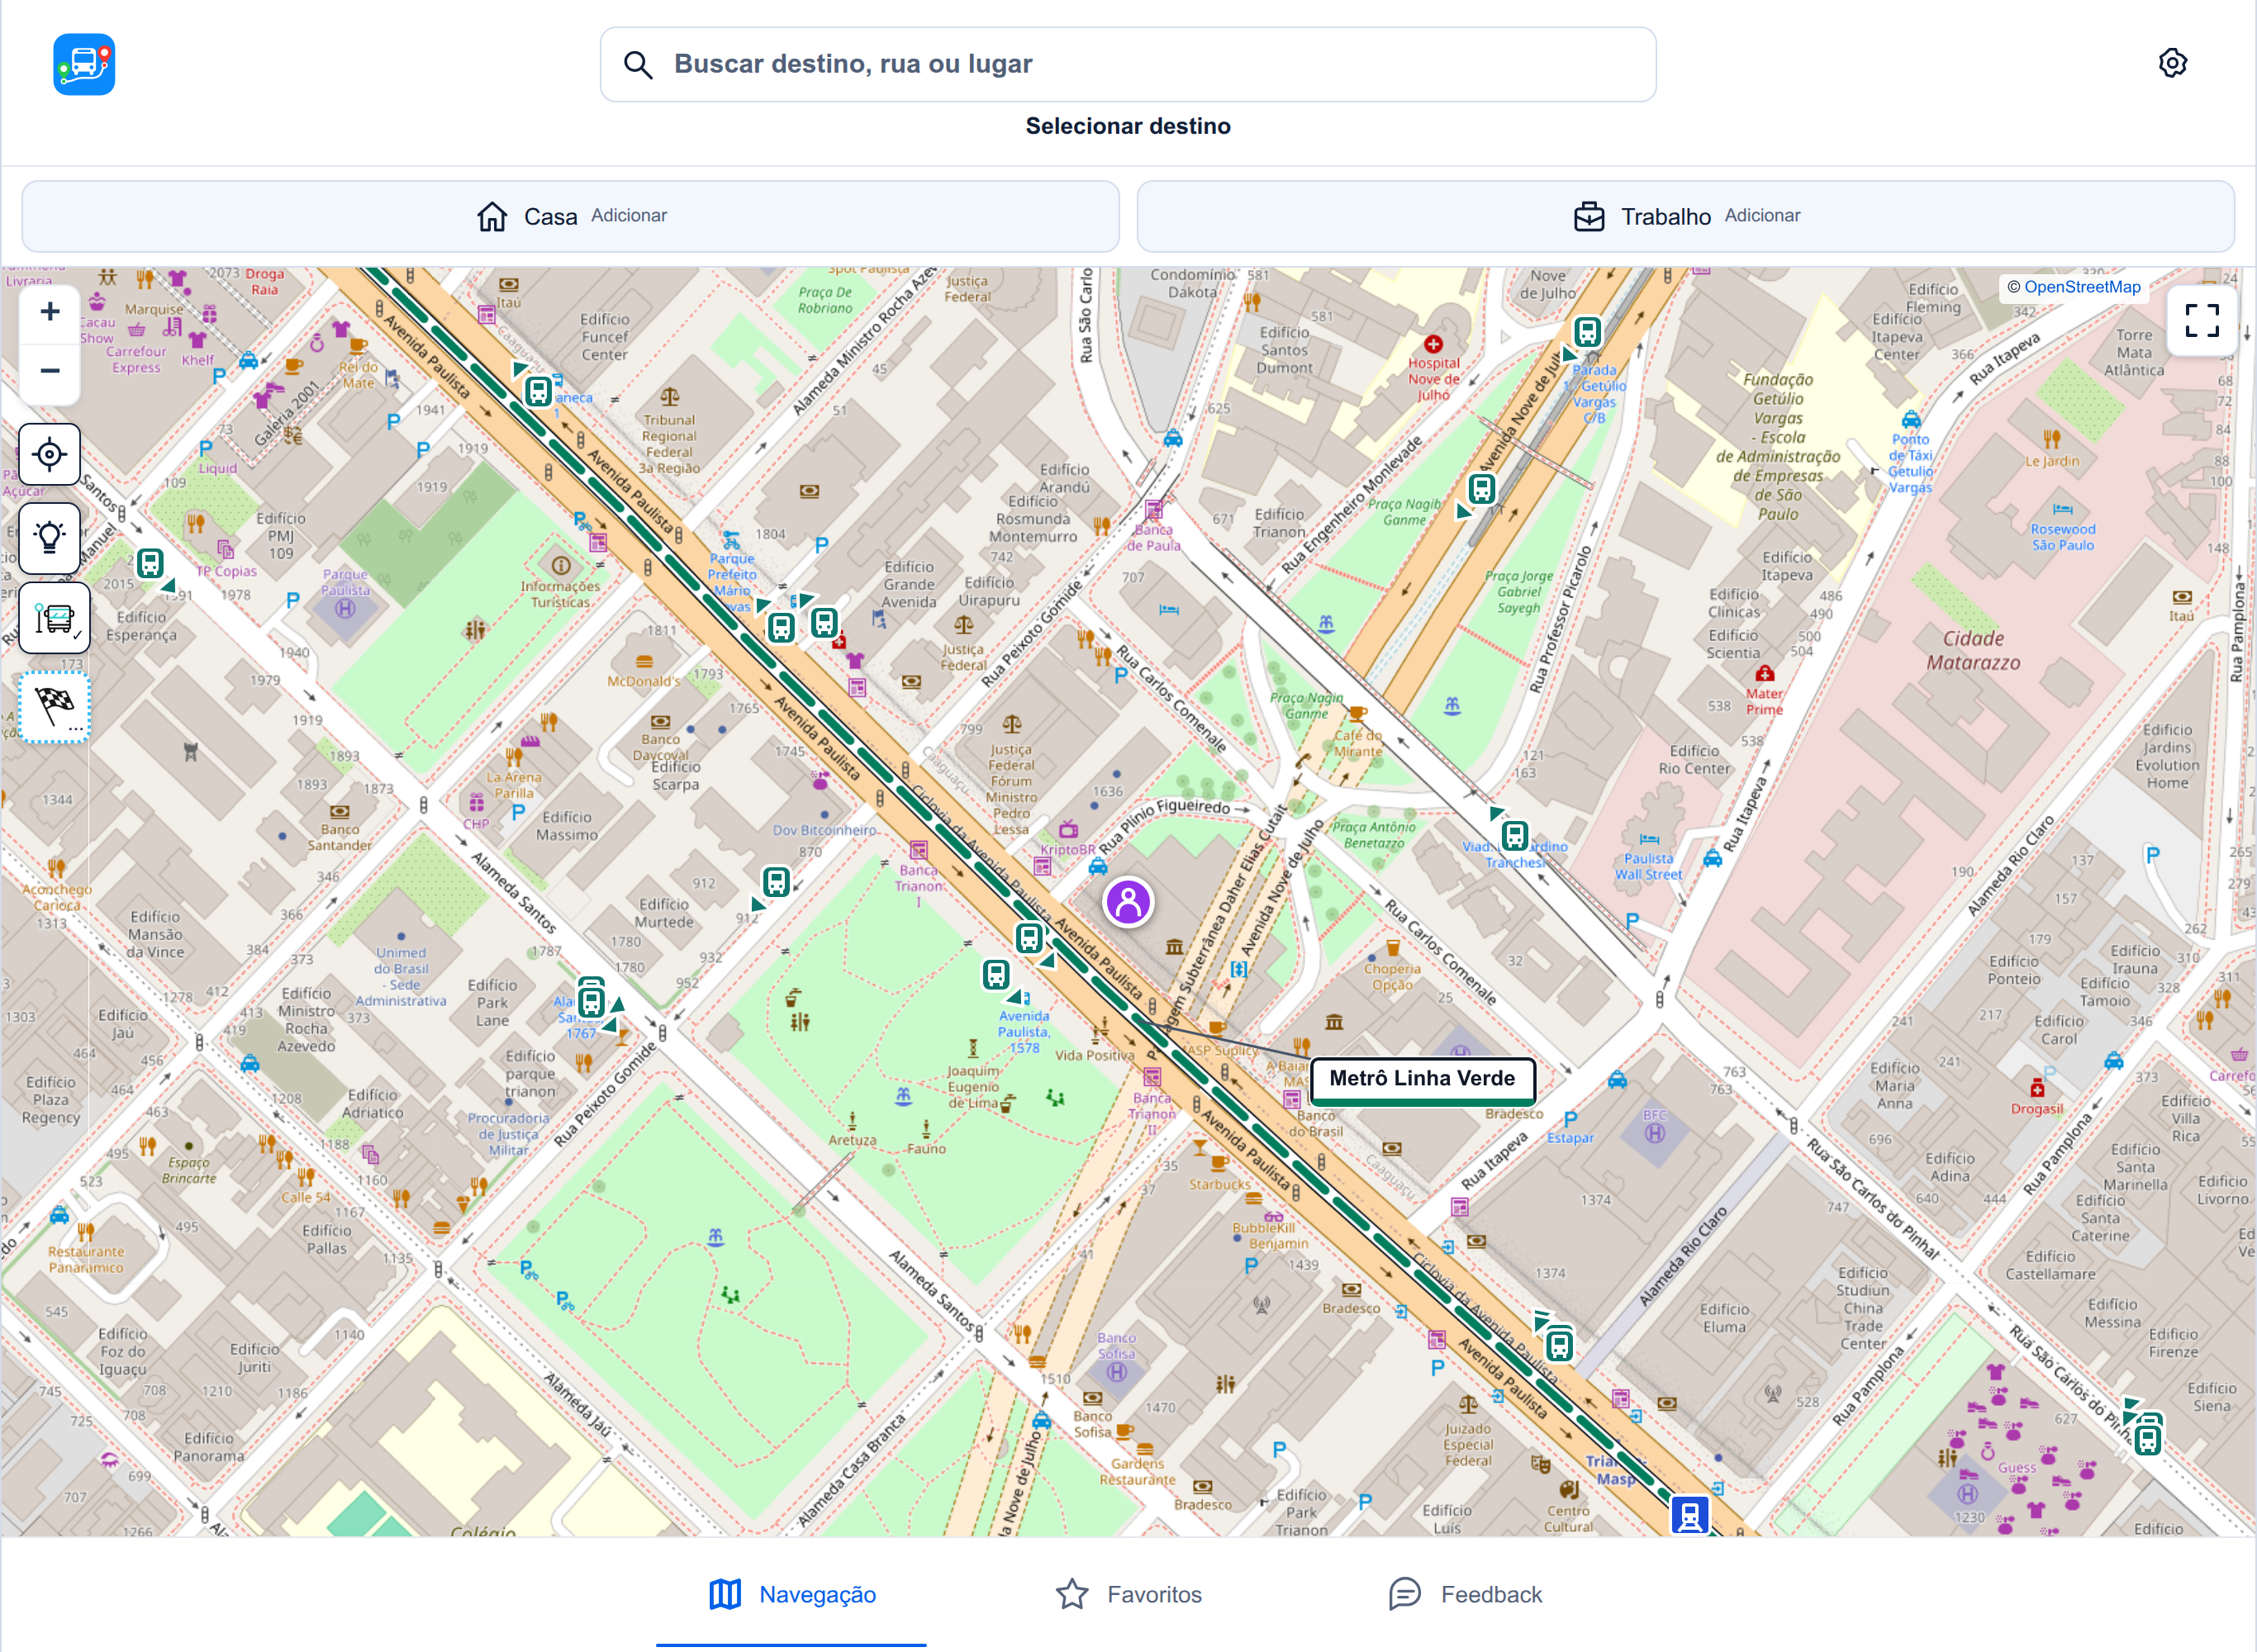
\includegraphics[width=\textwidth,height=0.43\textheight,keepaspectratio]{capturas/2026-11-02-interface-atual/ferrovia-light.png}
\caption{Identificação ferroviária atual no tema claro: mapa colorido e um rótulo para a Linha Verde.}\label{fig:contraste-ferroviario}
\fonte{Captura da revisão 78e3935, 2 nov. 2026; lâmpada acesa e localização simulada no MASP.}
\end{figure}
\begin{figure}[H]\centering
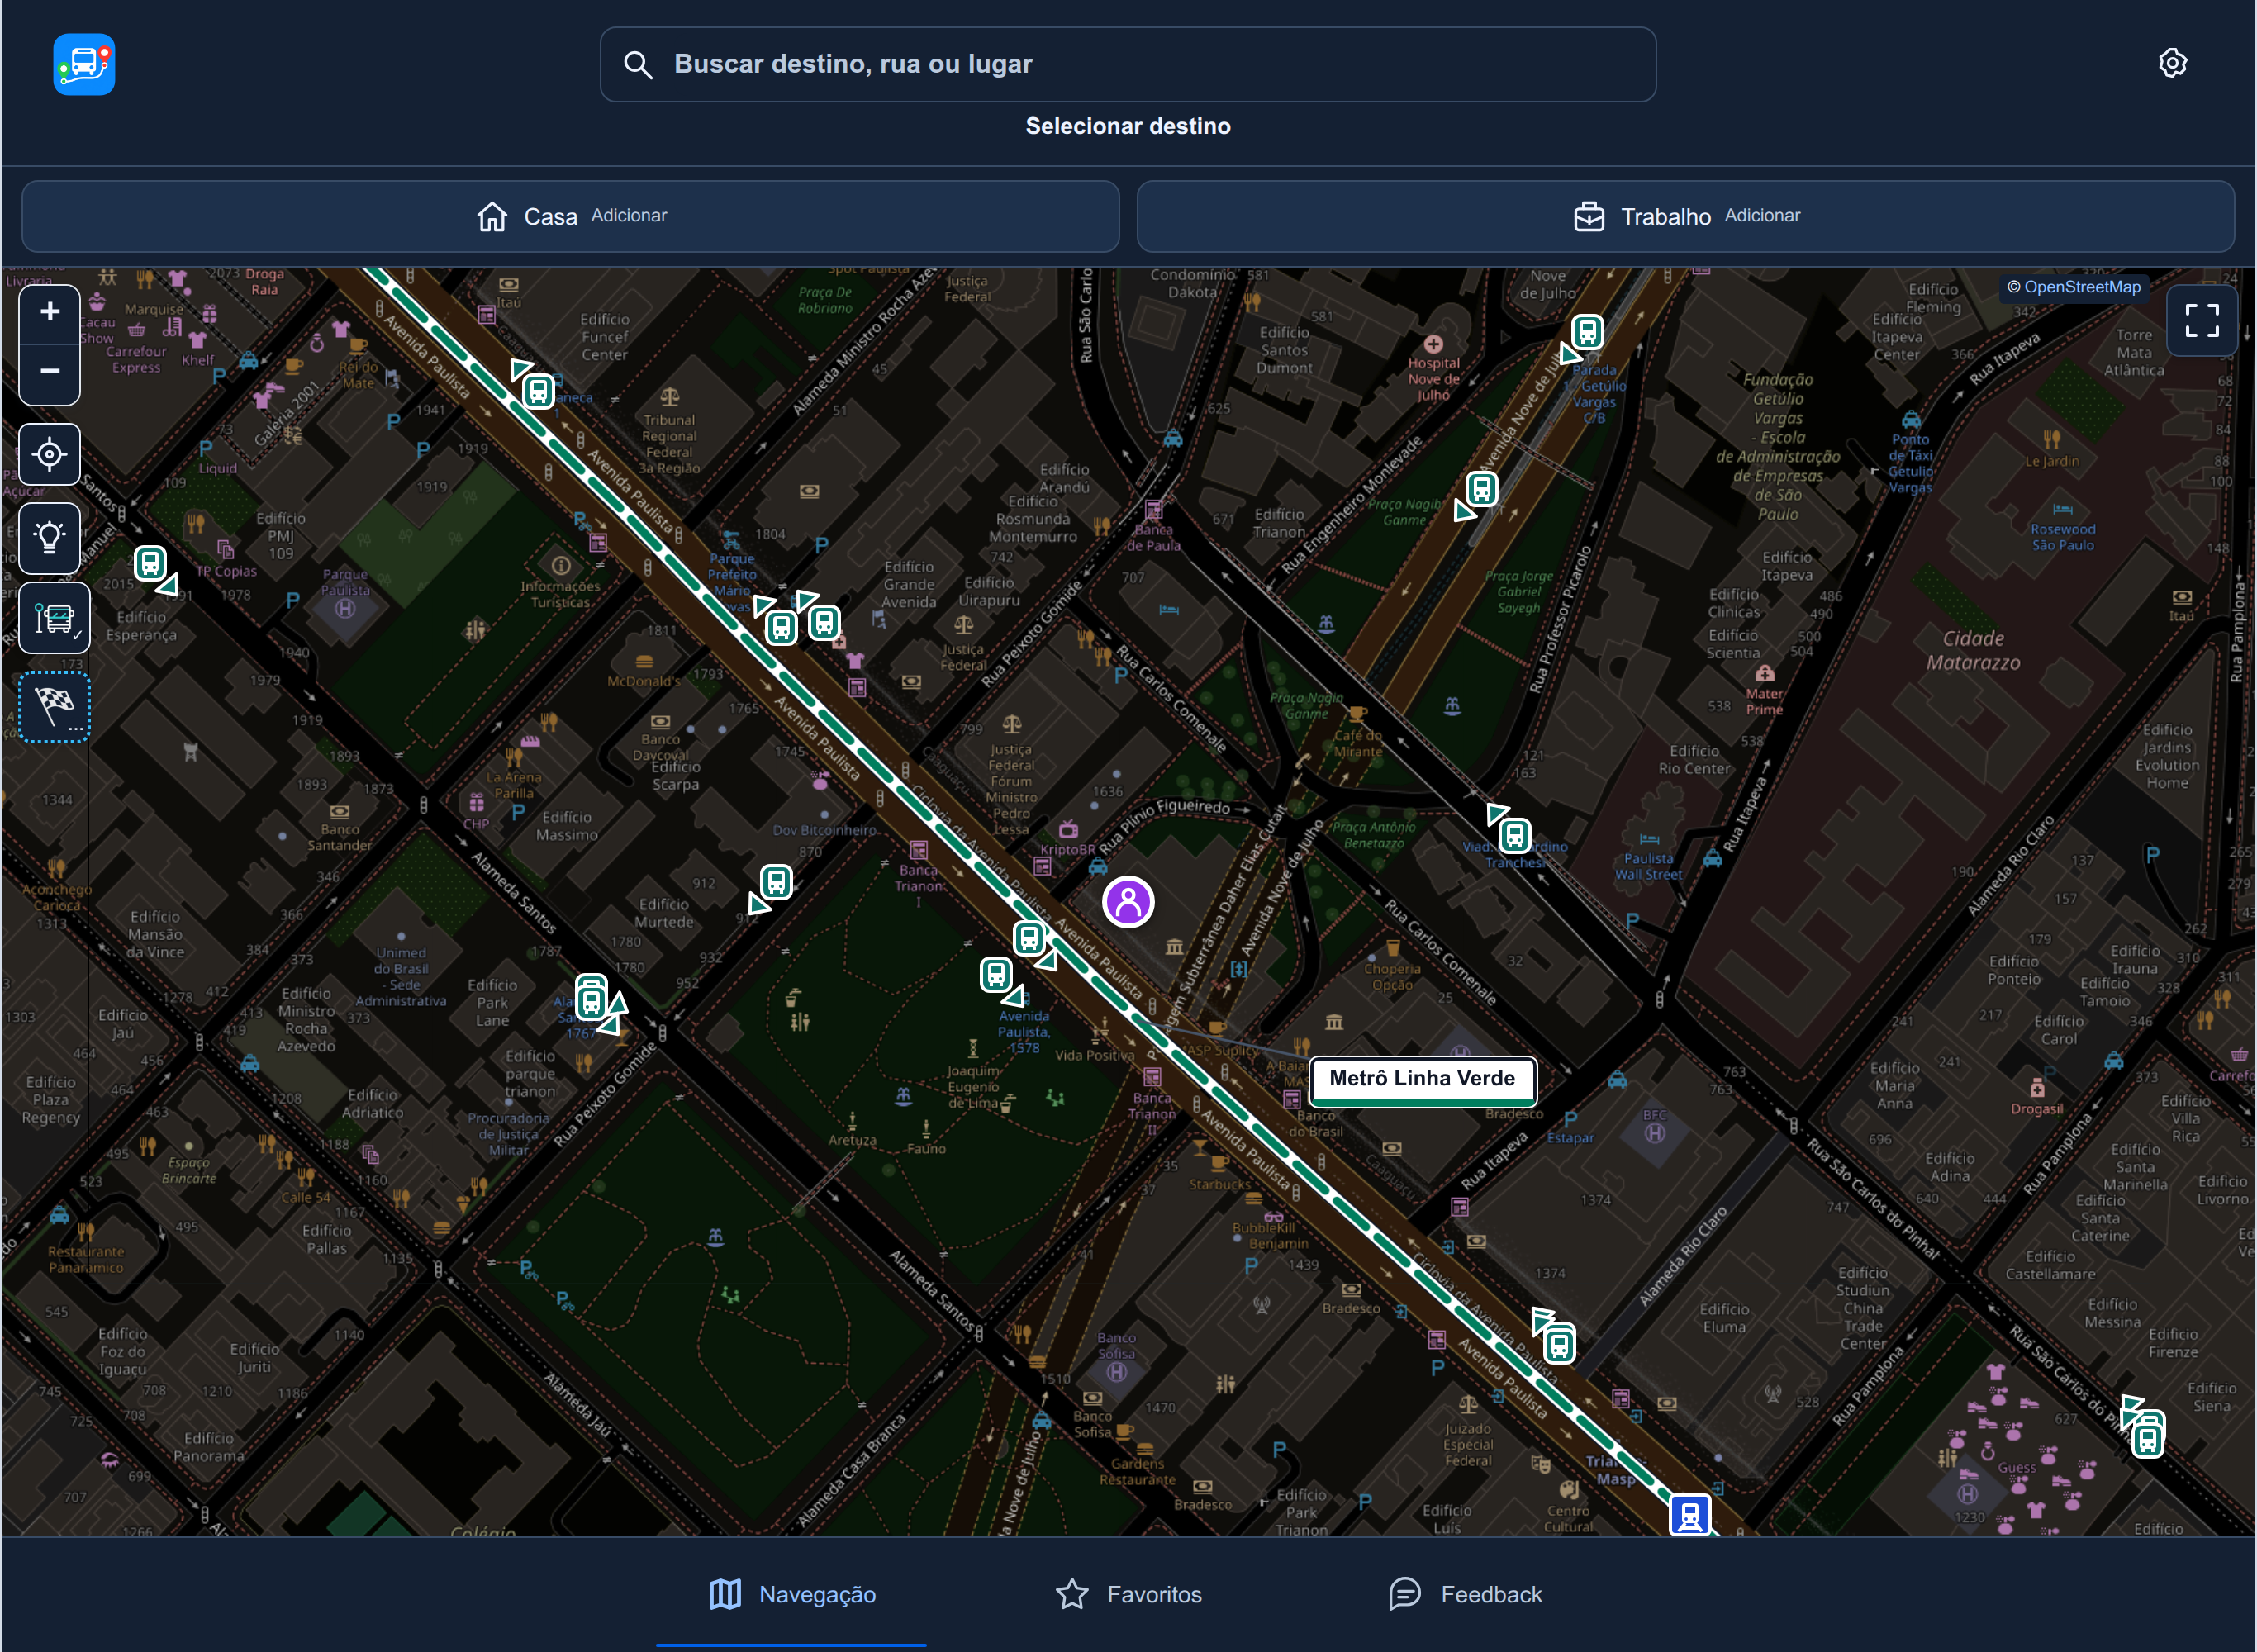
\includegraphics[width=\textwidth,height=0.43\textheight,keepaspectratio]{capturas/2026-11-02-interface-atual/ferrovia-dark.png}
\caption{Identificação ferroviária atual no tema escuro, com o mesmo enquadramento no MASP.}\label{fig:contraste-ferroviario-escuro}
\fonte{Captura da revisão 78e3935, 2 nov. 2026; lâmpada acesa, sem retoque da imagem.}
\end{figure}

A conferência técnica incluiu opacidade, identificadores, mudança de tema, enquadramento e interação com os pontos, além de captura em tela móvel. Os testes automatizados executados não substituem avaliação de compreensão, conforto visual ou acessibilidade com passageiros. Trata-se de correção implementada e verificada tecnicamente, ainda sujeita à avaliação por tarefas prevista para a continuidade do projeto. As Figuras~\ref{fig:contraste-ferroviario} e~\ref{fig:contraste-ferroviario-escuro} documentam a revisão 78e3935 da interface, recapturada em 2 de novembro, sem alterar os resultados históricos dos estudos anteriores.


\section{IHC, limitações e ameaças à validade}\label{sec:validade}

A matriz da Tabela~\ref{tab:ihc-evidencias} liga princípios discutidos na fundamentação às decisões observáveis. Não é uma avaliação heurística independente nem um escore de usabilidade: explicita a hipótese de benefício e a evidência necessária para verificá-la.
\begingroup\small\SingleSpacing\setlength{\parskip}{0pt}\setlength{\tabcolsep}{4pt}
\begin{longtable}{>{\raggedright\arraybackslash}p{2.8cm}p{4.0cm}p{4.2cm}p{3.5cm}}
\caption{Princípios de IHC, decisões, evidências e limitações.}\label{tab:ihc-evidencias}\\\hline
Princípio & Decisão implementada & Evidência & Limitação\\\hline\endfirsthead
\hline Princípio & Decisão implementada & Evidência & Limitação\\\hline\endhead\hline\endfoot
Reconhecimento em vez de memorização & Origem contextual e escolha por destino; favoritos locais. & Capturas de embarque, destino e favoritos; estudo de cliques no Apêndice~\ref{ap:cliques}. & Não mede compreensão ou esforço cognitivo dos passageiros.\\[4pt]
Visibilidade do estado & Progresso da busca, resultados parciais e previsão indisponível explicitados. & Capturas, testes registrados e aviso na Figura~\ref{fig:artesp-onibus-trem}. & Usuário pode confundir programação com previsão; reconhecimento ainda deve ser medido.\\[4pt]
Controle e recuperação & Recálculo manual, confirmação do cancelamento, preservação dos favoritos. & Requisitos e rastreabilidade no Apêndice~\ref{ap:engenharia}. & Teste automatizado não mede erros reais de uso ou compreensão do diálogo.\\[4pt]
Prevenção de erros & Seleção por toque prolongado cancelada em arrasto; distinção de embarque, destino e sentido. & Relatos e correções da Tabela~\ref{tab:feedback-ajustes}. & Episódios exploratórios não equivalem a incidência de erro em uma amostra.\\[4pt]
Hierarquia e redundância visual & Contraste, contornos e identificação textual ferroviária; controle de marcadores. & Seção~\ref{sec:legibilidade-ferroviaria}; capturas e verificações locais. & Não há validação de acessibilidade com participantes de diferentes percepções de cor.\\[4pt]
Liberdade de participação & Consulta ao transporte independente da gravação e comando de interrupção. & Fluxo de pesquisa e inspeção do código; Figura~\ref{fig:pesquisa-voluntaria}. & Consentimento implementado não garante anonimato ou conformidade legal integral.\\
\end{longtable}
\fonte{Síntese do grupo a partir da fundamentação de IHC e das evidências indicadas; revisão de 2 nov. 2026.}
\endgroup
\subsection{Ameaças à validade e alcance das conclusões}\label{sec:ameacas-validade}
\textbf{Validade interna.} Os benchmarks comparam consultas pareadas, mas não isolam variáveis de hardware, carga, cache do sistema operacional e escalonamento. A associação entre revisão e tempos observados não demonstra o efeito causal de uma técnica específica. Testes com respostas controladas verificam contratos, sem reproduzir toda a variabilidade de serviços externos.

\textbf{Validade externa.} A seleção estratificada de casos difíceis não representa a distribuição de viagens do município. Medições locais excluem rede, túnel e celular; datas e horários escolhidos não cobrem toda a operação. Relatos de desenvolvedores e convidados, bem como a apreciação de um profissional, não generalizam benefícios à população.

\textbf{Validade de construção.} Cliques não equivalem a esforço cognitivo; primeira rota não equivale a melhor rota; cobertura estrutural não equivale a viagem viável; intenção de deslocamento não equivale a embarque. Custo ponderado, quantidade de baldeações, frequência, programação e previsão são medidas diferentes. A redução de esforço requer sucesso correto, compreensão e observação de uso, não apenas menos ações.

\textbf{Atualização e qualidade dos dados.} GTFS representa cadastro e programação. O recorte ARTESP usa calendário de 2026 sem exceções de feriados e horários intermediários interpolados. Limites territoriais e coordenadas próximos à divisa exigem leitura cuidadosa; o mapa não homologa localização ou acesso em campo. Previsões operacionais dependem de correspondência segura e disponibilidade da fonte. Dados novos exigirão nova auditoria; o censo de 1/11 não descreve a base ampliada de 2/11.

\textbf{Reprodutibilidade.} Arquivos individuais, scripts e hashes permitem recalcular figuras e estatísticas. Entretanto, o HEAD observado com alterações locais não identifica sozinho o código executado, e não foi localizado manifesto contemporâneo completo da carga e de todos os fontes do benchmark. A revisão preserva essa lacuna. O apêndice técnico registra parâmetros e assinaturas disponíveis; não se reconstruíram medições nem condições ausentes.

\textbf{Avaliação com passageiros.} A entrevista de gestão, a avaliação profissional e as navegações exploratórias são contribuições distintas. Não há avaliação sistemática concluída que demonstre redução de esforço, tempo, espera ou erros para passageiros. Permanecem necessários consentimento, definição de amostra, tarefas equivalentes e registro de compreensão. A leitura física do QR e a implantação autorizada da sinalização também exigem evidências próprias.

Os limites de retenção, exclusão e exportação da pesquisa estão na Seção~\ref{sec:avaliacao-privacidade}; sua implementação não comprova anonimato ou conformidade legal integral.


\chapter{Considerações finais}
A pergunta de pesquisa foi como apoiar a pessoa no ponto de ônibus a reconhecer alternativas para chegar ao destino sem conhecer previamente as linhas ou a identificação da parada. O PaP responde tecnicamente com uma aplicação web que integra identificação contextual do embarque, escolha por destino, comparação de alternativas e visualização dos trechos e transferências, sem instalação obrigatória. A contribuição está nesse encadeamento implementado e documentado; não na alegação de novidade de QR Code, favoritos ou planejamento por destino, já presentes em outras soluções.

A escuta da gestão de Mauá delimitou o problema e as condições de acesso aos dados. O demonstrador histórico permaneceu separado da implementação com GTFS da SPTrans e Olho Vivo. Em 2 de novembro, a integração ARTESP ampliou a aplicação ao contexto metropolitano de Mauá: 337 paradas, 16 linhas ou variantes e 705, 427 e 359 viagens programadas distintas nos dias de referência, além de conexões com a ferrovia. O mapa e a captura de ônibus 157 com Linha 10 documentam cadastro e funcionamento do planejamento, sem comprovar execução da viagem, integração de todos os ônibus municipais ou cobertura da população.

Os resultados técnicos são mensuráveis, mas têm universos diferentes. O censo de 1 de novembro encontrou 99,666\% de cobertura estrutural dos pares anteriores à ARTESP. No benchmark local, entre 1.637 sucessos pareados, a mediana aumentou de 0,282 para 0,599 s, o P95 caiu de 5,698 para 5,143 s e o máximo de 10,712 para 5,936 s. A melhora da cauda coexistiu com regressão da mediana e não ocorreu uniformemente nos estratos. Os arquivos individuais sustentam essas descrições, sem demonstrar causalidade técnica, latência completa no celular ou benefício de usabilidade.

A apreciação da Alameda Solutions sobre as versões de outubro e os relatos exploratórios contribuíram para a revisão da clareza, do controle e da prevenção de erros. O parecer assinado foi preservado e sua procedência distinguida da consolidação editorial; alterações de novembro não são atribuídas ao avaliador. As decisões implementadas são coerentes com os princípios de IHC discutidos, conforme a matriz da Seção~\ref{sec:validade}, mas coerência de projeto e avaliação qualitativa não substituem resultados empíricos com passageiros.

O objetivo geral foi, portanto, parcialmente alcançado. Há solução funcional, integração de fontes e evidências técnicas e qualitativas; não há demonstração empírica de redução do esforço, da espera ou dos erros dos passageiros. Também não foi comprovada a leitura física do QR pelo protocolo proposto. Os limites internos, externos, de construção, atualização, reprodução e participação estão reunidos na Seção~\ref{sec:ameacas-validade}.

A continuidade deve priorizar tarefas consentidas com passageiros, registro físico da leitura do QR, validação de acessos e cadastro com os responsáveis locais e medição da cadeia completa no celular. A atualização de calendários, a investigação dos pares sem cobertura, a limpeza independente da coleta e o tratamento das exportações de pesquisa também permanecem necessários. A eventual implantação da sinalização depende de autorização e manutenção. A contribuição à comunidade é uma solução verificável e uma base para essa avaliação; seu impacto efetivo permanece uma questão aberta, a ser respondida com evidências de uso.

\postextual
\begin{thebibliography}{99}
\SingleSpacing\raggedright
\bibitem[{ARTESP}(2026)]{artespgtfs2026} ARTESP. \textit{GTFS: dados de transporte metropolitano}. Pacote versão 20261007. São Paulo, 2026. Disponível em: \url{https://dadosabertos.artesp.sp.gov.br/dataset/gtfs}. Acesso em: 2 nov. 2026.
\bibitem[{Barbosa \textit{et al.}}(2021)]{barbosa2021} BARBOSA, S. D. J.; SILVA, B. S.; SILVEIRA, M. S.; GASPARINI, I.; DARIN, T.; BARBOSA, G. D. J. \textit{Interação Humano-Computador e Experiência do Usuário}. Rio de Janeiro: Autopublicação, 2021. Disponível em: \url{https://leanpub.com/ihc-ux}. Acesso em: 7 out. 2026.
\bibitem[{Bast \textit{et al.}}(2015)]{bast2015} BAST, Hannah \textit{et al.} \textit{Route planning in transportation networks}. 2015. Preprint. arXiv:1504.05140. DOI: \url{https://doi.org/10.48550/arXiv.1504.05140}. Disponível em: \url{https://arxiv.org/abs/1504.05140}. Acesso em: 7 out. 2026.
\bibitem[{Batz \textit{et al.}}(2013)]{batz2013} BATZ, Gernot Veit; GEISBERGER, Robert; SANDERS, Peter; VETTER, Christian. Minimum time-dependent travel times with contraction hierarchies. \textit{Journal of Experimental Algorithmics}, [\textit{s. l.}], v. 18, n. 1, art. 1.4, abr. 2013. DOI: \url{https://doi.org/10.1145/2444016.2444020}. Disponível em: \url{https://publikationen.bibliothek.kit.edu/1000139527}. Acesso em: 8 out. 2026.
\bibitem[{Baum \textit{et al.}}(2019)]{baum2019} BAUM, Moritz; BUCHHOLD, Valentin; SAUER, Jonas; WAGNER, Dorothea; ZÜNDORF, Tobias. UnLimited TRAnsfers for Multi-Modal Route Planning: An Efficient Solution. \textit{In}: ANNUAL EUROPEAN SYMPOSIUM ON ALGORITHMS (ESA), 27., 2019, Munich/Garching. \textit{Proceedings [...]}. Dagstuhl: Schloss Dagstuhl -- Leibniz-Zentrum für Informatik, 2019. (Leibniz International Proceedings in Informatics, v. 144). p. 14:1--14:16. DOI: \url{https://doi.org/10.4230/LIPIcs.ESA.2019.14}. Disponível em: \url{https://drops.dagstuhl.de/entities/document/10.4230/LIPIcs.ESA.2019.14}. Acesso em: 8 out. 2026.
\bibitem[{Brakewood; Watkins}(2019)]{brakewood2019} BRAKEWOOD, C.; WATKINS, K. A literature review of the passenger benefits of real-time transit information. \textit{Transport Reviews}, [\textit{s. l.}], v. 39, n. 3, p. 327--356, maio 2019. DOI: \url{https://doi.org/10.1080/01441647.2018.1472147}. Disponível em: \url{https://candacebrakewood.com/wp-content/uploads/2019/05/brakewood-and-watkins-preprint-paper.pdf}. Acesso em: 5 out. 2026.
\bibitem[{C4 model}({[20\mbox{-}\mbox{-}]})]{c4container} C4 MODEL. \textit{Container diagram}. [20\mbox{-}\mbox{-}]. Disponível em: \url{https://c4model.com/diagrams/container}. Acesso em: 7 out. 2026.
\bibitem[{Card, Moran e Newell}(1980)]{card1980} CARD, Stuart K.; MORAN, Thomas P.; NEWELL, Allen. The keystroke-level model for user performance time with interactive systems. \textit{Communications of the ACM}, [New York], v. 23, n. 7, p. 396--410, jul. 1980. DOI: \url{https://doi.org/10.1145/358886.358895}. Disponível em: \url{https://iihm.imag.fr/blanch/ens/2010-2011/M1/EIHM/cours/1980-Card-KLM.pdf}. Acesso em: 26 out. 2026.
\bibitem[{Chacon; Straub}(2014)]{git} CHACON, Scott; STRAUB, Ben. \textit{Pro Git}. 2. ed. Berkeley, CA: Apress, 2014. Disponível em: \url{https://git-scm.com/book/pt-br/v2}. Acesso em: 23 set. 2026.
\bibitem[{Cittamobi}(2022)]{cittamobiajuda} CITTAMOBI. \textit{Como o Cittamobi funciona?} Central de Ajuda. 2022. Disponível em: \url{https://cittamobi.zendesk.com/hc/pt-br/articles/9379145018519-Como-o-Cittamobi-funciona}. Acesso em: 24 set. 2026.
\bibitem[{Cittamobi}({[20\mbox{-}\mbox{-}]})]{cittamobimaua} CITTAMOBI. \textit{Suzantur -- Mauá: horários de ônibus, linhas, itinerários e paradas}. [20\mbox{-}\mbox{-}]. Disponível em: \url{https://linhas.cittamobi.com.br/linhas/estado/sao-paulo/maua/suzantur-maua}. Acesso em: 24 set. 2026.
\bibitem[{Delling; Pajor; Werneck}(2012)]{delling2012} DELLING, Daniel; PAJOR, Thomas; WERNECK, Renato F. Round-based public transit routing. \textit{In}: MEETING ON ALGORITHM ENGINEERING AND EXPERIMENTS (ALENEX), 14., 2012, Kyoto. \textit{Proceedings [...]}. Philadelphia: SIAM, 2012. p. 130--140. DOI: \url{https://doi.org/10.1137/1.9781611972924.13}. Disponível em: \url{https://www.microsoft.com/en-us/research/publication/round-based-public-transit-routing/}. Acesso em: 7 out. 2026.
\bibitem[{Design Council}({[20\mbox{-}\mbox{-}]})]{designcouncil} DESIGN COUNCIL. \textit{Framework for Innovation}. [20\mbox{-}\mbox{-}]. Disponível em: \url{https://www.designcouncil.org.uk/resources/framework-for-innovation/}. Acesso em: 24 set. 2026.
\bibitem[{Dibbelt \textit{et al.}}(2018)]{dibbelt2018} DIBBELT, Julian; PAJOR, Thomas; STRASSER, Ben; WAGNER, Dorothea. Connection scan algorithm. \textit{Journal of Experimental Algorithmics}, [\textit{s. l.}], v. 23, art. 1.7, out. 2018. DOI: \url{https://doi.org/10.1145/3274661}. Disponível em: \url{https://publikationen.bibliothek.kit.edu/1000088435}. Acesso em: 8 out. 2026.
\bibitem[{Dijkstra}(1959)]{dijkstra1959} DIJKSTRA, E. W. A note on two problems in connexion with graphs. \textit{Numerische Mathematik}, [\textit{s. l.}], v. 1, p. 269--271, dez. 1959. DOI: \url{https://doi.org/10.1007/BF01386390}. Disponível em: \url{https://link.springer.com/article/10.1007/BF01386390}. Acesso em: 7 out. 2026.
\bibitem[{Django Software Foundation}({[20\mbox{-}\mbox{-}]})]{django} DJANGO SOFTWARE FOUNDATION. \textit{Django documentation}. Versão 6.0. [20\mbox{-}\mbox{-}]. Disponível em: \url{https://docs.djangoproject.com/en/6.0/}. Acesso em: 23 set. 2026.
\bibitem[{Equipe do Projeto Integrador II}(2026a)]{planoacao2026} EQUIPE DO PROJETO INTEGRADOR II. \textit{Plano de ação: Projeto Integrador em Computação II}. [\textit{S. l.}]: Universidade Virtual do Estado de São Paulo, 2026a. Documento acadêmico não publicado.
\bibitem[{Equipe do Projeto Integrador II}(2026b)]{mbmimportacoes} EQUIPE DO PROJETO INTEGRADOR II. \textit{Ponto a Ponto: importações externas e localização aproximada das paradas}. [\textit{S. l.}]: Equipe do Projeto Integrador II, 2026b. Documento técnico não publicado, atualizado em 24 set. 2026.
\bibitem[{Google}(2026)]{androidapplinks} GOOGLE. \textit{About deep links}. Android Developers. 2026. Disponível em: \url{https://developer.android.com/training/app-links}. Acesso em: 24 set. 2026.
\bibitem[{Gutteridge}(2012)]{southampton} GUTTERIDGE, Christopher. \textit{Study of QR Codes in Southampton Bus Stops}. Southampton Open Data Blog, 27 mar. 2012. Disponível em: \url{https://blog.soton.ac.uk/data/2012/03/27/studey-of-qr-codes-in-southampton-bus-stops/}. Acesso em: 23 set. 2026.
\bibitem[{Hart; Nilsson; Raphael}(1968)]{hart1968} HART, P. E.; NILSSON, N. J.; RAPHAEL, B. A Formal Basis for the Heuristic Determination of Minimum Cost Paths. \textit{IEEE Transactions on Systems Science and Cybernetics}, [\textit{s. l.}], v. 4, n. 2, p. 100--107, 1968. DOI: \url{https://doi.org/10.1109/TSSC.1968.300136}. Disponível em: \url{https://ieeexplore.ieee.org/document/4082128/}. Acesso em: 7 out. 2026.
\bibitem[{Haylett}(2018)]{haylett2018} HAYLETT, Amanda Jane. \textit{Improving the clarity of travel information for familiar and unfamiliar travellers in public transport travel information systems}. 2018. Tese (Doctor of Engineering) -- Faculty of Engineering and the Environment, University of Southampton, Southampton, 2018. Disponível em: \url{https://eprints.soton.ac.uk/455573/}. Acesso em: 7 out. 2026.
\bibitem[{IBGE}(2024)]{ibgemalha2024} IBGE. \textit{Malha municipal 2024: São Paulo}. Rio de Janeiro, 2024. Disponível em: \url{https://geoftp.ibge.gov.br/organizacao_do_territorio/malhas_territoriais/malhas_municipais/municipio_2024/UFs/SP/SP_Municipios_2024.zip}. Acesso em: 2 nov. 2026.
\setlength{\bibsep}{\baselineskip}
\interlinepenalty=10000
\bibitem[{IDEO}({[20\mbox{-}\mbox{-}]})]{ideo-designthinking} IDEO. \textit{What is design thinking?} [20\mbox{-}\mbox{-}]. Disponível em: \url{https://designthinking.ideo.com/introduction}. Acesso em: 24 set. 2026.
\bibitem[{International Organization for Standardization}(2025)]{iso25062} INTERNATIONAL ORGANIZATION FOR STANDARDIZATION. \textit{ISO 25062:2025}: Systems and software engineering --- Systems and software Quality Requirements and Evaluation (SQuaRE) --- Common Industry Format (CIF) for reporting usability evaluations. Geneva: ISO, jan. 2025. Disponível em: \url{https://www.iso.org/standard/84255.html}. Acesso em: 26 out. 2026.
\bibitem[{International Organization for Standardization}(2018)]{iso924111} INTERNATIONAL ORGANIZATION FOR STANDARDIZATION. \textit{ISO 9241-11:2018: Ergonomics of human-system interaction --- Part 11: Usability: Definitions and concepts}. Geneva: ISO, 2018. Disponível em: \url{https://www.iso.org/standard/63500.html}. Acesso em: 7 out. 2026.
\bibitem[{Laubheimer}(2019)]{laubheimer2019} LAUBHEIMER, Page. \textit{The 3-Click Rule for Navigation Is False}. Nielsen Norman Group, 11 ago. 2019. Disponível em: \url{https://www.nngroup.com/articles/3-click-rule/}. Acesso em: 26 out. 2026.
\bibitem[{MDN Web Docs}(2026a)]{geolocation} MDN WEB DOCS. \textit{Geolocation API}. Atualizado em 11 set. 2026a. Disponível em: \url{https://developer.mozilla.org/en-US/docs/Web/API/Geolocation_API}. Acesso em: 23 set. 2026.
\bibitem[{MDN Web Docs}(2026b)]{responsive} MDN WEB DOCS. \textit{Responsive web design}. Atualizado em 4 set. 2026b. Disponível em: \url{https://developer.mozilla.org/en-US/docs/Learn_web_development/Core/CSS_layout/Responsive_Design}. Acesso em: 23 set. 2026.
\bibitem[{MobilityData}({[20\mbox{-}\mbox{-}]})]{gtfs} MOBILITYDATA. \textit{General Transit Feed Specification: Overview}. [20\mbox{-}\mbox{-}]. Disponível em: \url{https://gtfs.org/documentation/overview/}. Acesso em: 23 set. 2026.
\bibitem[{Nielsen}(1994)]{nielsen1994} NIELSEN, Jakob. \textit{10 Usability Heuristics for User Interface Design}. Nielsen Norman Group, 24 abr. 1994. Revisado em 30 jan. 2024. Disponível em: \url{https://www.nngroup.com/articles/ten-usability-heuristics/}. Acesso em: 7 out. 2026.
\bibitem[{Nielsen}(2000)]{nielsen2000} NIELSEN, Jakob. \textit{Why You Only Need to Test with 5 Users}. Nielsen Norman Group, 18 mar. 2000. Disponível em: \url{https://www.nngroup.com/articles/why-you-only-need-to-test-with-5-users/}. Acesso em: 26 out. 2026.
\bibitem[{Norman}(2013)]{norman2013} NORMAN, D. A. \textit{The Design of Everyday Things}. Revised and expanded edition. New York: Basic Books, 2013. Disponível em: \url{https://jnd.org/books/the-design-of-everyday-things-revised-and-expanded-edition/}. Acesso em: 7 out. 2026.
\bibitem[{Object Management Group}(2017)]{uml251} OBJECT MANAGEMENT GROUP. \textit{Unified Modeling Language: version 2.5.1}. dez. 2017. Disponível em: \url{https://www.omg.org/spec/UML/2.5.1/About-UML}. Acesso em: 7 out. 2026.
\bibitem[{OpenStreetMap Foundation}({[20\mbox{-}\mbox{-}]})]{osmlicense} OPENSTREETMAP FOUNDATION. \textit{Direitos autorais e licença}. [20\mbox{-}\mbox{-}]. Disponível em: \url{https://www.openstreetmap.org/copyright?locale=pt}. Acesso em: 23 set. 2026.
\bibitem[{OpenStreetMap Wiki}(2026)]{osmpt} OPENSTREETMAP WIKI. \textit{Key:public\_transport}. Atualizado em 16 mar. 2026. Disponível em: \url{https://wiki.openstreetmap.org/wiki/Key:public_transport}. Acesso em: 23 set. 2026.
\bibitem[{OpenStreetMap Wiki}({[20\mbox{-}\mbox{-}]})]{overpass} OPENSTREETMAP WIKI. \textit{Overpass API}. [20\mbox{-}\mbox{-}]. Disponível em: \url{https://wiki.openstreetmap.org/wiki/Overpass_API}. Acesso em: 23 set. 2026.
\bibitem[{Pereira; Andrade; Vieira}(2023)]{pereira2023} PEREIRA, R. H. M.; ANDRADE, P. R.; VIEIRA, J. P. B. Exploring the time geography of public transport networks with the gtfs2gps package. \textit{Journal of Geographical Systems}, [\textit{s. l.}], v. 25, n. 3, p. 453--466, jul. 2023. DOI: \url{https://doi.org/10.1007/s10109-022-00400-x}. Disponível em: \url{https://www.urbandemographics.org/publication/2022_jgs_time_geography_gtfs2gps/}. Acesso em: 5 out. 2026.
\bibitem[{PostGIS Project}({[20\mbox{-}\mbox{-}]})]{postgis} POSTGIS PROJECT. \textit{PostGIS Manual}. [20\mbox{-}\mbox{-}]. Disponível em: \url{https://postgis.net/docs/en/}. Acesso em: 23 set. 2026.
\bibitem[{Prommaharaj \textit{et al.}}(2020)]{prommaharaj2020} PROMMAHARAJ, P.; PHITHAKKITNUKOON, S.; DEMISSIE, M. G.; KATTAN, L.; RATTI, C. Visualizing public transit system operation with GTFS data: a case study of Calgary, Canada. \textit{Heliyon}, [\textit{s. l.}], v. 6, n. 4, e03729, abr. 2020. DOI: \url{https://doi.org/10.1016/j.heliyon.2020.e03729}. Disponível em: \url{https://senseable.mit.edu/papers/pdf/20200320_Prommaharaj-etal_VisualizingTransit_Helyon.pdf}. Acesso em: 5 out. 2026.
\bibitem[{React}({[20\mbox{-}\mbox{-}]})]{react} REACT. \textit{React documentation}. [20\mbox{-}\mbox{-}]. Disponível em: \url{https://react.dev/}. Acesso em: 23 set. 2026.
\bibitem[{São Paulo (Município)}(2013)]{hackatona2013} SÃO PAULO (Município). \textit{Hackatona do Ônibus reúne jovens para desenvolvimento de aplicativos para o transporte}. 26 out. 2013. Disponível em: \url{https://prefeitura.sp.gov.br/w/noticia/hackatona-do-onibus-reune-jovens-para}. Acesso em: 23 set. 2026.
\bibitem[{São Paulo (Município)}(2014)]{qrsptrans2014} SÃO PAULO (Município). \textit{Nova tecnologia, QR Code já fornece informações por celular aos usuários de ônibus}. 24 jun. 2014. Disponível em: \url{https://prefeitura.sp.gov.br/web/mobilidade/w/noticias/173515}. Acesso em: 23 set. 2026.
\bibitem[{São Paulo Transporte S.A.}({[20\mbox{-}\mbox{-}]}a)]{sptransapi} SÃO PAULO TRANSPORTE S.A. \textit{API do Olho Vivo: guia de referência}. [20\mbox{-}\mbox{-}]a. Disponível em: \url{https://www.sptrans.com.br/desenvolvedores/api-do-olho-vivo-guia-de-referencia/documentacao-api/}. Acesso em: 23 set. 2026.
\bibitem[{São Paulo Transporte S.A.}({[20\mbox{-}\mbox{-}]}b)]{sptransadesivojs} SÃO PAULO TRANSPORTE S.A. \textit{Aplicação QRCodeAdesivo: adesivo.js}. Recurso público; cabeçalho HTTP Last-Modified consultado. [20\mbox{-}\mbox{-}]b. Disponível em: \url{http://qrcodeadesivo.extapps.sptrans.com.br/QRCodeAdesivo/adesivo.js?2021631733832}. Acesso em: 23 set. 2026.
\bibitem[{São Paulo Transporte S.A.}({[20\mbox{-}\mbox{-}]}c)]{sptranscss} SÃO PAULO TRANSPORTE S.A. \textit{Aplicação QRCodeAdesivo: GeneXusXEv2.css}. Recurso público; cabeçalho HTTP Last-Modified consultado. [20\mbox{-}\mbox{-}]c. Disponível em: \url{http://qrcodeadesivo.extapps.sptrans.com.br/QRCodeAdesivo/Resources/Portuguese/GeneXusXEv2.css?14585136}. Acesso em: 23 set. 2026.
\bibitem[{São Paulo Transporte S.A.}({[20\mbox{-}\mbox{-}]}d)]{sptransgxcfg} SÃO PAULO TRANSPORTE S.A. \textit{Aplicação QRCodeAdesivo: gxcfg.js}. Recurso público; cabeçalho HTTP Last-Modified consultado. [20\mbox{-}\mbox{-}]d. Disponível em: \url{http://qrcodeadesivo.extapps.sptrans.com.br/QRCodeAdesivo/gxcfg.js?54798}. Acesso em: 23 set. 2026.
\bibitem[{São Paulo Transporte S.A.}({[20\mbox{-}\mbox{-}]}e)]{sptransgxgral} SÃO PAULO TRANSPORTE S.A. \textit{Aplicação QRCodeAdesivo: gxgral.js}. Recurso público; cabeçalho HTTP Last-Modified consultado. [20\mbox{-}\mbox{-}]e. Disponível em: \url{http://qrcodeadesivo.extapps.sptrans.com.br/QRCodeAdesivo/gxgral.js?54798}. Acesso em: 23 set. 2026.
\bibitem[{São Paulo Transporte S.A.}({[20\mbox{-}\mbox{-}]}f)]{sptransparada70016782} SÃO PAULO TRANSPORTE S.A. \textit{Informações desta parada: Av. Paulista, n. 200, código 70016782}. [20\mbox{-}\mbox{-}]f. Disponível em: \url{http://qrcodeadesivo.extapps.sptrans.com.br/QRCodeAdesivo/adesivo.aspx?70016782}. Acesso em: 23 set. 2026.
\bibitem[{Sauro}(2012)]{sauro2012seq} SAURO, Jeff. \textit{10 Things To Know About The Single Ease Question (SEQ)}. MeasuringU, 30 out. 2012. Disponível em: \url{https://measuringu.com/seq10/}. Acesso em: 26 out. 2026.
\bibitem[{Sawin; Stahl; Sternisko}(2011--2012)]{transitplanner} SAWIN, Eugen; STAHL, Philip; STERNISKO, Jonas. \textit{Transit Planner: Basic Concepts}. Freiburg: Universität Freiburg, c2011--2012. Disponível em: \url{https://ad-publications.cs.uni-freiburg.de/student-projects/transfer-patterns-robustness/concepts.html}. Acesso em: 23 set. 2026.
\bibitem[{Sedgewick; Wayne}({[20\mbox{-}\mbox{-}]})]{sedgewicksp} SEDGEWICK, R.; WAYNE, K. \textit{Algorithms, 4th edition: 4.4 Shortest Paths}. [20\mbox{-}\mbox{-}]. Disponível em: \url{https://algs4.cs.princeton.edu/44sp/}. Acesso em: 23 set. 2026.
\bibitem[{Tullis; Albert}(2013)]{tullis2013} TULLIS, Tom; ALBERT, Bill. \textit{Measuring the user experience}: collecting, analyzing, and presenting usability metrics. 2nd ed. Waltham, MA: Morgan Kaufmann, 2013. DOI: \url{https://doi.org/10.1016/C2011-0-00016-9}. Disponível em: \url{https://www.sciencedirect.com/book/monograph/9780124157811/measuring-the-user-experience}. Acesso em: 26 out. 2026.
\bibitem[{Universidade Virtual do Estado de São Paulo}(2026)]{matriz2026} UNIVERSIDADE VIRTUAL DO ESTADO DE SÃO PAULO. \textit{Matriz Curricular do Aluno: Bacharelado em Tecnologia da Informação}. Matriz BT.INFORMACAO.1. [\textit{S. l.}]: UNIVESP, 7 out. 2026. 2 p. Documento institucional não publicado.
\end{thebibliography}


\chapter*{Glossário}
\addcontentsline{toc}{chapter}{GLOSSÁRIO}
\label{sec:glossario}
Este glossário reúne os principais termos técnicos e siglas utilizados no relatório. As definições indicam seu significado no contexto do Ponto a Ponto (PaP).

\begin{description}[style=nextline,leftmargin=0pt,labelwidth=0pt,font=\bfseries,itemsep=0.5\baselineskip]
\item[API (Application Programming Interface)] Interface pela qual sistemas trocam dados e solicitam operações. No PaP, permite que a interface React consulte os serviços Django.
\item[ARTESP] Agência de Transporte do Estado de São Paulo; fonte do cadastro e da programação metropolitana incorporados em 2 de novembro. Não é a fonte de previsões Olho Vivo.
\item[AVL (Automatic Vehicle Location)] Localização automática de veículos. Na extensão de São Paulo, posições da frota podem ser obtidas pela API Olho Vivo quando disponíveis e associadas com segurança aos registros utilizados pelo protótipo. No cenário histórico dos ônibus municipais de Mauá, os veículos demonstrativos permanecem simulados.
\item[Backend] Parte da aplicação executada no servidor, responsável pelas regras de negócio, acesso ao banco e respostas às consultas.
\item[Baldeação] Troca de veículo durante uma viagem. O planejamento considera o intervalo mínimo necessário para a conexão e a compatibilidade dos horários.
\item[Catálogo] Conjunto de registros de linhas, variantes, paradas e documentos importados. A presença no catálogo não garante que uma linha possua dados suficientes para o planejamento.
\item[Chave estrangeira (FK, Foreign Key)] Campo que referencia um registro de outra tabela, estabelecendo um vínculo no banco de dados.
\item[Chave primária (PK, Primary Key)] Campo ou combinação de campos que identifica de forma única cada registro de uma tabela.
\item[Cobertura cadastral, estrutural, temporal e operacional] Níveis distintos: presença no cadastro; existência de conexão modelada; viabilidade em uma data e horário; disponibilidade observada ou informada pela operação. Ver Tabela~\ref{tab:niveis-cobertura}.
\item[Design Thinking] Abordagem de projeto orientada às necessidades das pessoas, à exploração de alternativas e ao aprendizado com protótipos e avaliações. No PaP, organiza a relação entre escuta, definição do problema, decisões de solução, apreciação profissional e avaliação com passageiros ainda pendente.
\item[Diferença pareada] Tempo depois menos tempo antes para a mesma consulta com sucesso nas duas versões. Valor negativo indica menor tempo; não identifica sua causa.
\item[Distribuição acumulada empírica] Fração das observações com valor menor ou igual a um limiar; deriva dos valores individuais, sem supor uma distribuição teórica.
\item[Frontend] Parte da aplicação com a qual o passageiro interage no navegador, incluindo mapa, listas, filtros e detalhes da viagem.
\item[Geolocalização aproximada] Estimativa das coordenadas de uma parada com base em endereço, malha viária e sequência do itinerário. Não equivale a localização validada em campo.
\item[Grafo] Representação por vértices e arestas. No projeto, permite modelar conexões viárias e estados de viagem; os pesos representam distância ou tempo, conforme a etapa do processamento.
\item[GTFS (General Transit Feed Specification)] Especificação de dados de transporte público. GTFS Schedule organiza informações programadas; GTFS-Realtime complementa com atualizações, posições e alertas. SPTrans e ARTESP fornecem cadastros programados; sua importação não comprova integração operacional com os ônibus municipais de Mauá.
\item[JSON (JavaScript Object Notation)] Formato textual estruturado utilizado em respostas da API, arquivos de importação e metadados persistidos pelo projeto.
\item[Mediana e percentil 95 (P95)] Medidas de posição da distribuição. O P95 utiliza nesta análise a convenção do instrumento original, explicitada na Seção~\ref{sec:desempenho-revisado}; máximo é apenas o maior valor observado.
\item[Mockup] Representação visual da interface proposta, utilizada na prototipação. Por si só, não demonstra funcionamento.
\item[ORM (Object-Relational Mapping)] Mapeamento entre objetos da aplicação e tabelas do banco. No projeto, o ORM do Django é utilizado para persistir e consultar os registros no SQLite.
\item[OSM (OpenStreetMap)] Base geográfica colaborativa utilizada como fonte de ruas, endereços e elementos de transporte, sujeita a limitações de cobertura e atualização.
\item[OSRM (Open Source Routing Machine)] Motor de cálculo de percursos viários. No cenário São Paulo, o serviço FOSSGIS/OSRM a pé fornece os percursos de caminhada; as geometrias dos ônibus provêm do GTFS. Os percursos viários da demonstração histórica de Mauá não constituem itinerários de ônibus homologados.
\item[Overpass API] Serviço de consulta de objetos do OpenStreetMap por critérios como localização, tipo e atributos. Fornece os recortes preservados pelo projeto.
\item[PaP (Ponto a Ponto)] Nome e sigla do projeto apresentado neste relatório. Seu principal objetivo é o deslocamento facilitado entre origem e destino, sem exigir conhecimento prévio das linhas, da identificação da parada ou da organização da rede de transporte.
\item[QR Code (Quick Response Code)] Código bidimensional que, neste projeto, contém um endereço web associado à parada e permite identificar a origem da consulta.
\item[Simulação ou dados mockados] Uso de dados preparados para demonstrar ou testar comportamentos. No cenário histórico de Mauá, horários, tempos e posições dos veículos demonstrativos não representam a operação real. No cenário São Paulo, o PaP não utiliza essa simulação operacional: emprega dados GTFS da SPTrans e consulta previsões e posições pela API Olho Vivo quando disponíveis. Cenários automatizados de teste e coordenadas simuladas do passageiro podem ser utilizados para reprodução e verificação técnica.
\item[SQLite] Sistema de banco de dados utilizado no catálogo histórico de Mauá e, em índice separado, no cadastro GTFS do cenário São Paulo.
\item[Sucesso pareado] Consulta que retornou primeira rota nas duas versões comparadas; não significa que a rota foi realizada por um passageiro.
\item[UQ (Unique)] Indicação de restrição de unicidade no diagrama: impede repetição da combinação de valores especificada dentro de uma tabela.
\item[Validade de construção] Correspondência entre a medida utilizada e o conceito que se deseja avaliar; por exemplo, contagem de cliques não mede sozinha esforço ou compreensão.
\item[Variante de linha] Registro de um percurso ou configuração particular de uma linha. Sentidos e sequências distintos podem corresponder ao mesmo código comercial.

\item[Viagem programada distinta] Registro de viagem GTFS contado uma vez no dia de serviço, independentemente de quantas paradas atravessa. Não equivale a veículo único ou viagem observada.
\end{description}

\begin{apendicesenv}
\chapter{Percurso metodológico detalhado}\label{ap:percurso-metodologico}
Este apêndice preserva o detalhamento do percurso histórico e dos procedimentos da versão de 2 de novembro. A síntese que distingue execução e proposta está na Seção~\ref{sec:metodologia-revisada}. A interrupção de materialização referida abaixo pertence ao desenho histórico de outubro; o censo compacto posterior está na Seção~\ref{sec:atualizacao-20261101}.

A metodologia articula as etapas de ouvir e interpretar o contexto, criar e prototipar, implementar e testar, orientadas pelo Design Thinking. Essa abordagem parte das necessidades das pessoas, explora alternativas e utiliza protótipos para aprender por iteração, considerando também viabilidade técnica e condições de continuidade da solução \citep{ideo-designthinking}. O modelo Double Diamond distingue descoberta, definição, desenvolvimento e entrega, com possibilidade de retorno às etapas anteriores \citep{designcouncil}. Neste relatório, essas referências ajudam a organizar as decisões do PaP; não se afirma que o grupo tenha executado integralmente um protocolo formal dessas instituições.

A revisão de Haylett acrescenta critérios de clareza da informação e um protocolo de avaliação por tarefas. A descrição a seguir sistematiza o percurso registrado do projeto, distinguindo relatos da comunidade, observações do grupo sobre interfaces e dados, hipóteses de uso e evidências de implementação. O ciclo de validação com passageiros permanece aberto. Não há registro, nesta etapa, de oficina formal de ideação, mapa de empatia ou personas produzidos com participantes, e esses instrumentos não são apresentados como atividades realizadas.

A comparação foi ampliada por registros sobre Santos fornecidos pelo grupo: a resposta ao protocolo 7657-2026, uma conversa informal com uma passageira e a descrição de um vídeo de leitura do QR Code. Esses materiais foram tratados como fontes distintas. A resposta institucional informa a oferta do serviço; a conversa registra uma experiência individual; a descrição do vídeo delimita um fluxo observado pelo grupo. A síntese documental preserva essa distinção e a ausência de data e identificação do setor remetente na resposta reproduzida. Nenhum desses registros corresponde a uma sessão de avaliação do PaP.

Na ampliação de 2 de novembro de 2026, o grupo confrontou o GTFS metropolitano ARTESP, versão \texttt{20261007}, com a malha municipal detalhada IBGE de 2024, selecionando Mauá pelo código \texttt{3529401} \citep{artespgtfs2026,ibgemalha2024}. Foram incluídas as coordenadas de paradas contidas no polígono, inclusive sua borda, sem depender da presença de ``Mauá'' no nome da linha. A contagem mantém identificadores distintos, inclusive pontos em sentidos opostos; não os transforma em locais físicos únicos. Os 337 registros encontrados têm coordenadas distintas. Cinco pontos incluídos ficam a até 20 metros da divisa, e três externos também estão nessa faixa; a relação foi preservada para explicitar a sensibilidade à precisão das coordenadas e da malha.

A conferência independente dos CSV do ZIP original reproduziu os identificadores de paradas e viagens do banco importado. Contaram-se viagens distintas por \texttt{trip\_id} e data de serviço, com sequência completa de ao menos duas paradas distintas, horários válidos e não decrescentes, e embarque ou desembarque no recorte municipal. Uma viagem que passa por várias paradas foi contada uma única vez; os registros ferroviários por frequência foram contabilizados separadamente. Foram examinados 3, 7 e 8 de novembro de 2026, representando dia útil, sábado e domingo, e consultas às 08h nesses dias, além de controles na madrugada e após a vigência ARTESP. O leitor de candidatos da aplicação foi executado com os bancos reais em modo somente leitura, mantendo calendários, caminhadas e limites de busca. Os horários de consulta foram parâmetros explícitos, não observações da circulação dos veículos. A procedência, os hashes e as condições de reprodução constam do Apêndice~\ref{ap:importacao}; os resultados estão na Seção~\ref{sec:artesp-maua}.


\label{sec:escuta-comunidade}
Na etapa de ouvir e interpretar o contexto, Osmar Junior, gerente de Transportes Públicos de Mauá, foi escolhido como interlocutor da comunidade externa por sua experiência no setor, pelo conhecimento da operação local e pela disponibilidade para colaborar com o projeto. Na entrevista, relatou atuação no transporte público desde 1985, predominantemente em Mauá, com trajetória na administração pública e em empresas operadoras  (entrevista com Osmar Junior, 257--284 s; 424--447 s).

Sua experiência contribui para esclarecer os sistemas e dados disponíveis, discutir a viabilidade da proposta e dialogar com os responsáveis pela operação. A comunidade beneficiária compreende os passageiros do transporte público de Mauá; o interlocutor contribui com a perspectiva profissional da gestão e da operação. Sua participação complementa a escuta dos usuários, mas não substitui os testes com passageiros nem implica, por si só, formalização de parceria ou autorização institucional.

A escuta inicial foi realizada em conversa remota entre um integrante do grupo, responsável pela entrevista, e o interlocutor. O registro foi incorporado ao projeto como transcrição com identificação de falantes e marcações temporais. O nome do arquivo indica 20 de agosto de 2026, às 14h00min44s, e a transcrição alcança 2.861 segundos, aproximadamente 47 minutos e 41 segundos. A data é a identificação do registro fornecido pelo grupo, não uma verificação independente dos metadados da gravação  (entrevista com Osmar Junior).

A análise da entrevista utiliza sínteses temáticas e intervalos em segundos para permitir a localização das passagens citadas. Os relatos operacionais foram tratados como informações da entrevista, não como cadastro oficial.

O interlocutor informou que o monitoramento dos veículos e a consulta pelo passageiro já existiam em Mauá. A conversa ajudou a delimitar a proposta como uma oportunidade de aprimorar o acesso contextualizado às informações disponíveis, sem pressupor a criação de um novo sistema de rastreamento. Ele avaliou favoravelmente a ideia de iniciar a consulta pelo QR Code da parada e sugeriu organizar a proposta por escrito e apresentá-la à empresa responsável pelo rastreamento  (entrevista com Osmar Junior, 447--589 s; 739--853 s; 1135--1163 s).

Ao discutir integração, o interlocutor distinguiu informações destinadas ao público de dados utilizados pela prefeitura e pela operadora. Não confirmou a existência de API acessível ao projeto. Ao final, dispôs-se a procurar um contato da empresa e a colaborar com a continuidade do trabalho. Essas manifestações indicam encaminhamentos para articulação, sem comprovar entrega de credenciais, assinatura de parceria ou autorização de implantação  (entrevista com Osmar Junior, 861--919 s; 2293--2425 s).

\clearpage
A~Tabela~\ref{tab:entrevista-osmar} registra a relação entre os temas da entrevista e as decisões do grupo. As implicações de projeto são interpretações da equipe, não requisitos formalmente aprovados pelo interlocutor.

\begingroup
\small\SingleSpacing
\setlength{\parskip}{0pt}
\setlength{\tabcolsep}{4pt}
\renewcommand{\arraystretch}{1.12}
\begin{longtable}{>{\raggedright\arraybackslash}p{0.17\textwidth}>{\raggedright\arraybackslash}p{0.35\textwidth}>{\raggedright\arraybackslash}p{0.39\textwidth}}
\caption{Contribuições da entrevista inicial e implicações para o PaP}\label{tab:entrevista-osmar}\\
\hline
Intervalo do registro & Tema discutido & Implicação delimitada pelo grupo \\
\hline
\endfirsthead
\multicolumn{3}{l}{\small Tabela \thetable{} -- continuação}\\
\hline
Intervalo do registro & Tema discutido & Implicação delimitada pelo grupo \\
\hline
\endhead
\hline\multicolumn{3}{r}{\small Continua na próxima página}\\
\endfoot
\hline
\multicolumn{3}{p{0.95\textwidth}}{\footnotesize Fonte: síntese do grupo a partir da transcrição da entrevista  (entrevista com Osmar Junior); intervalos em segundos.}\\
\endlastfoot
181--222; 739--853 & Monitoramento existente e receptividade à consulta pelo ponto físico. & Priorizar QR Code associado à parada e acesso simples; avaliar a compreensão com passageiros.\\
\hline
773--795 & Referência aproximada a 1.600 paradas e distinção entre ponto de parada e abrigo. & Não condicionar o cadastro à existência de abrigo; conferir identificação, local e autorização da sinalização. A estimativa oral não valida a contagem importada.\\
\hline
861--919; 1135--1163; 2293--2425 & Separação entre informações públicas e internas; sugestão de apresentação e contato com o fornecedor. & Documentar a proposta, solicitar cadastro e condições de integração; manter, no cenário de Mauá, a simulação enquanto o acesso operacional não estiver confirmado.\\
\hline
1647--1785 & Discussão de anúncio das paradas e orientação de quem desconhece o percurso. & Considerar legibilidade e identificação de embarque e desembarque na avaliação; anúncio sonoro embarcado permanece fora da entrega atual.\\
\hline
2499--2543 & Programação por ordem de serviço e diferenças entre dias úteis, sábados e domingos. & Solicitar calendários e horários por tipo de dia para integração futura; o cenário demonstrativo de Mauá não representa a programação vigente.\\
\hline
2583--2679 & Efeitos do trânsito, chuva e alagamentos sobre a operação. & Distinguir horário programado de previsão; explicitar indisponibilidade e atualização dos dados. No cenário de Mauá, Dijkstra com tempos simulados não mede atrasos operacionais.\\
\end{longtable}
\endgroup

Também foram levantadas, pelo entrevistador, ideias de relatos de lotação com pontuação e de orientação sonora de paradas. Essas possibilidades integram a exploração inicial de alternativas, mas não foram incorporadas como funcionalidades entregues ou compromissos de implementação. O recorte atual concentra-se no acesso web pelo ponto e no planejamento por destino  (entrevista com Osmar Junior, 112--153 s; 1647--1785 s).


A entrevista com o interlocutor documenta receptividade à ideia, informações sobre o contexto operacional e sugestões de encaminhamento, anteriores à avaliação da interface. As capturas do QRCodeAdesivo e do Olho Vivo constituem observações documentais de fluxos específicos, enquanto a cobertura incompleta das fontes públicas é uma constatação técnica do levantamento. A hipótese de que o passageiro desconheça a linha adequada, tenha dificuldade para interpretar muitas opções ou necessite de ajuda em uma baldeação ainda deverá ser investigada com usuários. A familiaridade tratada por Haylett fundamenta essa investigação, sem substituir evidências locais.

O desafio de projeto foi delimitado como: \textit{como ajudar uma pessoa que está no ponto de ônibus a reconhecer alternativas para chegar ao destino, sem precisar conhecer previamente linhas ou a identificação da parada?} A necessidade central é compreender o deslocamento. O QR Code é uma resposta proposta para identificar a origem; a seleção do destino, a comparação de alternativas e as instruções de troca respondem às decisões seguintes.

Para ampliar a escuta, a próxima etapa deverá investigar com passageiros como escolhem o ônibus, reconhecem o sentido e lidam com conexões; com o interlocutor e responsáveis pelo serviço, deverá verificar quais dados existem e quem pode mantê-los. Datas, participantes, perguntas e observações deverão ser registrados com consentimento, distinguindo a fala ou o comportamento observado da interpretação do grupo.

A análise das telas do Cittamobi complementou a entrevista inicial: enquanto a entrevista indicou a existência de monitoramento e consulta por aplicativo em Mauá, as capturas examinadas mostraram busca por destino e planejamento com conexões. O grupo reviu, assim, a interpretação de sua contribuição: essas funcionalidades passaram a compor o fluxo proposto, sem serem apresentadas como diferenciais inéditos. Nesse momento, a hipótese principal passou a ser a utilidade de identificar a parada física por QR Code e iniciar a consulta com esse contexto já definido. Os registros posteriores sobre Santos levaram a examinar a continuidade desse acesso até a seleção do destino. Essa revisão exemplifica o retorno da pesquisa à definição do problema; sua utilidade para os passageiros ainda deverá ser avaliada.

Com esse recorte, a prototipação busca tornar a proposta compreensível e permitir que a comunidade discuta o fluxo, suas limitações e as condições de uso antes de uma implantação real.

Foram produzidos mockups conceituais e implementado o PaP com Django, React, Leaflet e SQLite. O fluxo associa o QR Code à origem, apresenta alternativas e permite escolher o destino e consultar um percurso. As imagens geradas automaticamente documentam a intenção de interface, enquanto o código e os testes documentam a implementação. Favoritos locais apoiam consultas recorrentes; não se desenvolve aplicativo Android nesta etapa.

Durante a etapa de prototipação, o grupo também utilizou o Figma para representar a navegação e discutir a organização inicial das telas. Esse mockup cumpriu uma função intermediária no desenvolvimento da solução. Com a evolução da aplicação Django/React para o protótipo funcional apresentado neste relatório, a própria aplicação passou a constituir a principal referência para revisão da experiência de uso e para as avaliações futuras. O mockup no Figma e as imagens conceituais permanecem como registros da evolução do projeto, e não como representação da versão final da interface.

No levantamento histórico de Mauá, a preparação dos dados compreendeu coleta e preservação das fontes, normalização de identificadores e sequências, importação no banco e geolocalização aproximada dos registros sem coordenadas. Fonte, data, evidências e pendências são mantidas para revisão. Nesse cenário de Mauá, os horários e veículos utilizados na demonstração são mantidos separadamente do cadastro público. A administração controla a ativação, o relógio e a velocidade dessa simulação; a interface do passageiro informa a natureza demonstrativa desses dados.

Na etapa de criar e prototipar, o grupo comparou alternativas de acesso, apresentação e integração. As decisões descritas a seguir resultaram do desenvolvimento e da pesquisa, sem constituírem uma oficina de cocriação com passageiros.
Quanto ao acesso, priorizou-se o acesso web por QR Code para iniciar a consulta sem instalação. Android permanece uma evolução futura; favoritos locais atendem inicialmente às consultas recorrentes.

Para apoiar a decisão de viagem, manteve-se a consulta das linhas do ponto, mas acrescentou-se o destino como filtro. A intenção é reduzir a exigência de conhecimento prévio, preservando a possibilidade de comparação.

Na apresentação dos percursos, a comparação reúne alternativas relevantes; o mapa de uma linha permanece como detalhamento. A análise dos serviços da SPTrans motivou essa escolha, sem demonstrar superioridade de usabilidade do PaP.

Na demonstração histórica de Mauá, adotaram-se geometrias viárias para tornar o caminho mais interpretável, sem homologação operacional desses percursos. No cenário São Paulo, o PaP utiliza as geometrias dos ônibus cadastradas no GTFS e o serviço de roteamento a pé para as caminhadas.

Diante das lacunas dos dados disponíveis para Mauá, optou-se, naquele cenário, por uma simulação identificada, controlada na administração, para apresentar o fluxo sem tratar horários fictícios como previsões operacionais. No cenário São Paulo, essa dependência de simulação foi superada pelo cadastro GTFS da SPTrans e pela integração com a API Olho Vivo, respeitados os limites de cobertura e disponibilidade.

Os critérios adotados foram acesso inicial simples, clareza para escolher o deslocamento, viabilidade com os dados disponíveis e possibilidade de repetir a demonstração. A manutenção do cadastro, a autorização para sinalização física e a disponibilidade de dados operacionais continuam condicionantes de implantação, e não resultados resolvidos pela escolha tecnológica.

O material registra a passagem da concepção de acesso pelo ponto para mockups visuais e, em seguida, para uma aplicação web interativa. As revisões do cenário de Mauá acrescentaram a organização das alternativas por destino, trajetos sobre ruas, controle administrativo da simulação e favoritos no navegador. A incorporação de fontes públicas e de coordenadas aproximadas naquele cenário levou à separação entre catálogo, inferência geográfica e demonstração. Essas mudanças decorreram de decisões do desenvolvimento e de limitações técnicas identificadas; ainda não são resultados de testes com passageiros.

A~Tabela~\ref{tab:design-thinking} relaciona as bases dessas decisões aos requisitos e à avaliação proposta. A coluna de validação descreve atividades futuras com a comunidade; a implementação existente, por si só, não confirma as hipóteses de uso.

\begingroup
\small
\setlength{\tabcolsep}{4pt}
\setlength{\parskip}{0pt}
\renewcommand{\arraystretch}{1.15}
\begin{longtable}{>{\raggedright\arraybackslash}p{0.23\textwidth}>{\raggedright\arraybackslash}p{0.20\textwidth}>{\raggedright\arraybackslash}p{0.25\textwidth}>{\raggedright\arraybackslash}p{0.23\textwidth}}
\caption{Relação entre observações, necessidades, decisões e validação proposta}\label{tab:design-thinking}\\
\hline
Observação ou hipótese & Necessidade interpretada & Solução proposta ou implementada & Forma de validação prevista \\
\hline
\endfirsthead
\multicolumn{4}{l}{\small Tabela \thetable{} -- continuação}\\
\hline
Observação ou hipótese & Necessidade interpretada & Solução proposta ou implementada & Forma de validação prevista \\
\hline
\endhead
\hline\multicolumn{4}{r}{\small Continua na próxima página}\\
\endfoot
\hline
\multicolumn{4}{p{0.95\textwidth}}{\footnotesize Fonte: elaboração do grupo a partir da entrevista inicial, das capturas analisadas e das decisões documentadas do PaP (2026).}\\
\endlastfoot
Entrevista registra interesse do interlocutor no acesso pelo ponto; o desconhecimento da parada pelo passageiro permanece hipótese de uso.
& Iniciar a consulta a partir do local físico.
& QR Code identifica a origem e abre o navegador; acesso implementado, implantação física pendente.
& Solicitar consulta sem fornecer nome da parada ou linha; observar conclusão e pedidos de ajuda.\\
\hline
Nas capturas do Olho Vivo, a lista por ponto apresenta várias linhas e o mapa mostra uma linha selecionada.
& Reconhecer quais alternativas atendem ao destino, sem conhecer previamente seus códigos.
& Filtragem por destino e comparação de alternativas; no cenário São Paulo, planejamento baseado no GTFS.
& Pedir que o participante escolha uma opção e explique por que ela o leva ao destino.\\
\hline
Hipótese de dificuldade para interpretar sentido, percurso e trocas; motivada também pela leitura de Haylett.
& Compreender onde embarcar, trocar e desembarcar.
& Etapas e baldeações simuladas em Mauá; no cenário São Paulo, trajetos GTFS e caminhadas calculadas.
& Solicitar explicação do percurso; registrar erros de sentido e de identificação da troca.\\
\hline
Hipótese de repetição de destinos como Casa, Trabalho e Escola.
& Reutilizar consultas sem limitar destinos novos.
& Favoritos opcionais no navegador; Android adiado.
& Salvar e reutilizar um destino, depois escolher outro; observar ações e dificuldades.\\
\hline
Levantamento de Mauá constatou lacunas de coordenadas e ausência de integração operacional confirmada.
& Distinguir informação disponível, aproximada e simulada.
& Em Mauá, catálogo separado, posições sinalizadas como aproximadas e simulação administrada fora da tela principal.
& Pedir que o participante identifique a natureza dos dados; com os responsáveis, conferir cadastro e atualização.\\
\end{longtable}
\endgroup

\label{sec:conversao}
A solução final utiliza o cadastro GTFS da SPTrans, importado em índice SQLite separado, e consultas ao Olho Vivo quando há correspondência segura de linha e parada. Essa escolha superou, no cenário de São Paulo, a dependência de reconstruir coordenadas por endereço encontrada no levantamento inicial de Mauá \citep{mbmimportacoes}. O Apêndice~\ref{ap:importacao} concentra a organização dos dados e a reprodução da importação. A busca de endereços e o roteamento a pé complementam o cadastro, sem substituir suas coordenadas ou confundir horários programados com previsões.

\label{sec:implementar-testar}
Na etapa de implementar e testar, o planejamento no cenário São Paulo começou pela busca por rodadas sobre viagens e horários GTFS, com caminhadas de acesso, transferência e saída. Os custos de processamento observados motivaram a investigação da materialização exaustiva dos percursos. A evolução adotou conexões estruturais reutilizáveis, índices diretos e reversos e composição bidirecional offline, seguida da materialização seletiva de candidatos. A consulta principal passou a recuperar esses candidatos para avaliação temporal, preservando o planejador por rodadas como fallback.

% Ajuste local: manter o parágrafo completo, sem alterar margens ou espaçamento.
\begin{samepage}
Essa evolução descreve decisões de projeto e mecanismos implementados, não um ganho global de desempenho já demonstrado. A interrupção por falta de espaço em disco refere-se à arquitetura histórica de 28 de outubro de 2026, posteriormente substituída, no fluxo atual, pela materialização compacta documentada na Seção~\ref{sec:atualizacao-20261101}. O protocolo da Seção~\ref{sec:benchmark-hibrido} permanece proposto para uma comparação futura sob condições equivalentes, em infraestrutura compatível. Os critérios de custo, validação e encerramento estão no Apêndice~\ref{ap:rotas}; os registros de testes de cada versão permanecem no Apêndice~\ref{ap:engenharia}, separados da avaliação com passageiros.
\par\end{samepage}

% Conteúdo independente para a revisão estilística v2: engenharia_metodologia
A documentação de engenharia foi organizada retrospectivamente a partir do código existente. A~Tabela~\ref{tab:requisitos-pap} sintetiza comportamentos e qualidades pretendidos, sem constituir uma especificação formal previamente aprovada. A Figura~\ref{fig:arquitetura-pap} apresenta as responsabilidades dos componentes. Diagramas comportamentais e a rastreabilidade detalhada estão no Apêndice~\ref{ap:engenharia}.
\begin{table}[H]\centering\small
\caption{Síntese dos requisitos da extensão São Paulo.}\label{tab:requisitos-pap}
\begin{tabular}{p{1.5cm}p{11.5cm}}\hline
ID & Comportamento ou qualidade pretendida\\\hline
RF01 & Identificar o embarque pela localização, pelo QR Code ou pela seleção manual.\\
RF02 & Consultar partidas e distinguir previsão operacional de horário ou frequência programados.\\
RF03 & Planejar por destino com caminhada, espera e baldeações, aceitando coordenadas por toque prolongado.\\
RF04 & Comparar alternativas e abrir a rota ou um trecho no mapa.\\
RF05 & Salvar, renomear e remover favoritos locais, confirmando a remoção.\\
RF06 & Cancelar mediante confirmação, desmarcando embarque e destino e preservando os favoritos; retornar à seleção de embarque.\\
RF07 & Acompanhar posição do ônibus e previsão de embarque compatível com a caminhada, com atualização a cada 15 segundos.\\
RQ01 & Informar progresso sem perder a seleção ou redefinir o zoom.\\
RQ02 & Reduzir esforço de interação preservando compreensão e controle.\\\hline
\end{tabular}\fonte{Síntese do grupo baseada na implementação e nos objetivos de IHC.}
\end{table}

\begin{figure}[H]
\centering\resizebox{\textwidth}{!}{\begin{tikzpicture}[>=Stealth,font=\small,
box/.style={draw,rounded corners,align=center,execute at begin node={\hyphenpenalty=10000\exhyphenpenalty=10000},text width=5.4cm,minimum height=1cm,fill=blue!4},arr/.style={->,thick}]
\node[box] (orig) at (0,0) {GTFS, rede ferroviária e malha pedestre\\Fontes e parâmetros versionados};
\node[box] (prep) at (0,-2.0) {Preparação offline\\Conexões dirigidas e caminhadas verificadas};
\node[box] (mat) at (0,-4.3) {Materialização compacta\\por etapas\\Até 5 alternativas por par; custo até 4};
\node[box] (entrada) at (7,0) {Origem, destino e horário\\React/Leaflet $\leftrightarrow$ Django};
\node[box] (fontes) at (7,-2.0) {Produtores concorrentes\\Preparados e buscas complementares/RAPTOR};
\node[box] (av) at (7,-4.3) {Avaliação temporal e pedestre\\Limites próprios e dependências externas};
\node[box,fill=green!8] (res) at (7,-6.8) {Publicação progressiva\\da primeira rota\\Continuação das demais alternativas};
\foreach \a/\b in {orig/prep,prep/mat,entrada/fontes,fontes/av,av/res}{\draw[arr] (\a)--(\b);}
\draw[arr] (mat.east)--(3.5,-4.3)--(3.5,-2.0)--(fontes.west);
\node[align=center,text width=13cm,font=\footnotesize] at (3.5,-9.0) {Estado de 1 de novembro de 2026. Troca envolvendo ônibus: custo 1;\\troca interna metrô/trem: $1/3$. Cobertura estrutural não garante viagem em todo horário.\\Uma fonte externa não precisa bloquear a publicação de outra fonte válida.};
\end{tikzpicture}
}
\caption{Arquitetura híbrida do planejamento no cenário São Paulo.}\label{fig:arquitetura-pap}
\fonte{Elaboração do grupo; arquitetura concorrente e legibilidade revisadas em 1 nov. 2026.}
\end{figure}

A interface consome a API do backend e o mapa-base; os favoritos permanecem no navegador. O backend recupera candidatos preparados, valida os percursos a pé e avalia a viabilidade temporal, consultando serviços externos sem transferir credenciais operacionais para a interface. A composição bidirecional pertence ao pré-processamento; a busca por rodadas integra os produtores concorrentes quando habilitada, conforme a atualização de 1 de novembro no Apêndice~\ref{ap:rotas}. As setas resumem dependências lógicas e não descrevem uma topologia de implantação em produção. A integração externa está sujeita a indisponibilidade, que deve ser comunicada sem transformar informações programadas em previsões operacionais.

A verificação técnica abrange importação, preservação das sequências, estimativas por endereço, cálculo de trajetos, API, preferências e fluxos da interface. Em 29 de setembro de 2026, foram executados com sucesso 65 testes Django, dez testes JavaScript e 13 testes de navegador com Playwright, totalizando 88 testes sem falhas. A execução de navegador incluiu a compilação do frontend e utilizou SQLite temporário, sem alterar o banco principal. Foram utilizados os comandos \texttt{python backend/manage.py test transit}, \texttt{npm test} e \texttt{npm run test:e2e}, sobre o código da revisão \texttt{a60f290}. O ambiente utilizou Python 3.14.4, Django 6.0.8 e Node.js 22.22.1; este último difere da versão 24 indicada pelo projeto, embora a compilação e os testes tenham sido concluídos nesse ambiente. Os resultados e comandos estão registrados em \nolinkurl{docs/verificacoes/2026-09-29/README.md}. Esses resultados verificam comportamentos programados, não a precisão das coordenadas ou a utilidade do sistema para passageiros.

O planejamento deve permanecer verificável por cenários de viagem direta, baldeação, conexão perdida, permanência no mesmo veículo e ausência de caminho. A comparação com resultados calculados manualmente e o caso de uma partida posterior com chegada anterior permitem conferir a lógica temporal. Alterações futuras dos dados e do algoritmo exigirão repetição dos casos pertinentes.

Após a entrevista, o grupo recebeu, em 2 de setembro de 2026, uma resposta por e-mail de Osmar sobre bilhetagem e estimativas de desembarque. Esse esclarecimento complementou o levantamento do problema, sem avaliar as telas do protótipo. Em 5 de outubro, as novas tentativas de contato permaneciam sem resposta. Posteriormente, em 2 de novembro de 2026, Osmar manifestou aprovação à concepção do PaP, conforme o Anexo~\ref{an:manifestacao-osmar}, sem documentar teste da implementação. A ampliação da interlocução ocorreu com Thiago Almeida Amorim, da Alameda Solutions, por intermédio de Nathalia Almeida Amorim, com retornos em 21 e 25 de outubro. O protótipo funcional e o relatório constituíram os objetos dessa apreciação; o Figma permanece como registro da prototipação.

O procedimento de consolidação da avaliação externa reuniu o registro de feedback, a lista de melhorias levantadas pelo grupo, as navegações de usuários por ele relatadas e a documentação das versões. O registro contém 26 itens sobre navegação, leitura do mapa, informações de transporte, participação na pesquisa e clareza do relatório. Os critérios qualitativos foram clareza, visibilidade do estado, controle, prevenção de erros e redução de esforço. O grupo confirmou o exame dos itens e a assinatura do parecer. Não há, no acervo consultado, descrição suficiente do canal de envio dos materiais, duração da avaliação ou tarefas executadas por Thiago; esses elementos não são reconstruídos como se houvessem sido registrados.

Para confrontar o retorno com a implementação, foram examinados os comportamentos descritos, os registros de testes, as capturas e os pontos pertinentes do código. Por exemplo, a confirmação do cancelamento foi conferida nos componentes \texttt{SaoPaulo.jsx} e \texttt{CancelTripDialog.jsx}. A atualização de 25 de outubro usa como referências o aplicativo \texttt{85417bc} e o relatório \texttt{c18556c}; os identificadores completos estão no Apêndice~\ref{ap:feedback-alameda}. O commit do primeiro retorno não está identificado. Essa conferência foi realizada para consolidar o relatório e não é atribuída ao avaliador como execução independente de testes.

A análise separa a origem de cada ajuste da apreciação posterior de seu resultado. O registro disponível atribui as propostas ao grupo e às navegações por ele relatadas, e a avaliação favorável a Thiago. Na ausência de uma recomendação individualizada do avaliador, a alteração não é apresentada como tendo sido solicitada por ele. O ciclo documentado reúne identificação de dificuldades, implementação, verificação técnica e apreciação profissional; permanece aberta a avaliação sistemática com passageiros. A seguir, apresenta-se o protocolo previsto para essa continuidade.

A avaliação futura do esforço de interação deverá usar tarefas com origem e destino equivalentes, comparando a entrada contextualizada por QR Code com a indicação manual da origem. O registro deverá separar leitura do código, toques, digitação, retornos, erros de seleção, pedidos de ajuda e tempo de conclusão. Deverá também verificar se o participante reconhece o embarque, o sentido, a caminhada e a baldeação, além de recolher sua percepção de facilidade. Uma redução no número de ações somente será interpretada como favorável quando não prejudicar a conclusão correta e a compreensão. O procedimento é uma proposta de avaliação, ainda não executada, orientada pela relação entre eficácia, eficiência e satisfação \citep{iso924111}.

Uma nova consulta aos responsáveis pelo transporte de Mauá deverá registrar o que o interlocutor compreendeu da proposta, quais aspectos considerou úteis, o que modificaria, sua percepção de viabilidade e limitações, a contribuição do QR Code em relação ao acesso já oferecido pelo Cittamobi e as possibilidades de integração com o fornecedor. Para cada sugestão, o grupo deverá documentar a decisão de incorporá-la, adiá-la ou não adotá-la, com justificativa e indicação da alteração correspondente. Esses itens constituem um roteiro de coleta, não respostas já obtidas. O retorno profissional será analisado separadamente de testes de compreensão realizados com passageiros.

A continuidade proposta prevê apresentação aos responsáveis pelo transporte local e uma avaliação exploratória com passageiros que relatem diferentes graus de familiaridade com os trajetos, sem tratar essa familiaridade como característica fixa de cada pessoa. O protocolo proposto começa pela leitura do QR Code, sem fornecer previamente nomes de pontos ou linhas, e pela indicação de um destino. A identificação da mesma parada no aplicativo existente permitirá comparar ações, tempo, erros de sentido e pedidos de ajuda. Em seguida, o participante deverá comparar uma alternativa direta com outra que contenha baldeação e explicar sua escolha, identificando linha, sentido, local de embarque, eventual troca e desembarque.

A sessão prosseguirá com a alteração do destino, observando a coerência entre lista, mapa e detalhes e a atualização do resultado anterior. Também serão apresentadas uma posição aproximada e uma previsão indisponível, para verificar se são distinguidas de localização validada e ausência de ônibus. Por fim, o participante deverá salvar e reutilizar um favorito e demonstrar como escolher outro destino.

Serão registrados conclusão sem ajuda, tempo por tarefa, erros de interpretação, pedidos de auxílio e compreensão das etapas. Uma breve explicação do percurso pelo participante e uma escala de confiança de 1 a 5 complementarão a observação; essa escala é proposta pelo grupo, não um instrumento validado pela tese. Os resultados serão descritivos, com indicação do número e perfil dos participantes e das limitações da amostra. Confiança elevada não será considerada sucesso quando a interpretação estiver incorreta. A participação deverá ser voluntária e os registros minimizados e apresentados sem identificação pessoal.

Após cada sessão de avaliação, o grupo deverá registrar a versão do protótipo e o cenário utilizado, a tarefa proposta, o comportamento observado, a dificuldade relatada e a interpretação dos responsáveis pela análise. Cada alteração deverá indicar a evidência que a motivou e a tarefa a repetir. Erros que levem à escolha de sentido, embarque ou conexão inadequados terão prioridade sobre ajustes estéticos. Caso a dificuldade esteja na compreensão do problema ou na qualidade dos dados, o processo deverá retornar à escuta e à revisão dos requisitos, em vez de se limitar a modificar a interface.

A entrevista inicial forneceu retorno sobre a ideia, e a apreciação de Thiago acrescentou uma avaliação profissional do aplicativo e do relatório. A manifestação posterior de Osmar, em 2 de novembro de 2026, aprovou a concepção da proposta (Anexo~\ref{an:manifestacao-osmar}). A avaliação funcional com Osmar e os testes sistemáticos com passageiros não estão documentados como realizados. Os resultados dessas etapas futuras deverão ser confrontados com os critérios de Haylett e poderão exigir novas alterações. A precisão das previsões operacionais não foi avaliada por esses procedimentos: simulação de Mauá, testes de software e capturas de consultas ao Olho Vivo. A validação operacional das paradas, dos sentidos e dos itinerários será uma atividade distinta, dependente de cadastro autorizado e conferência pelos responsáveis pelo serviço.

\chapter{Protocolo pendente de leitura física do QR Code}\label{ap:protocolo-qr}
O acervo examinado contém abertura de URL, emulação de navegador, QR exibido na interface e uma ilustração de uso identificada em \nolinkurl{capturas/ilustracao-qr.txt}. Esses materiais não comprovam leitura física por câmera. O protocolo a seguir é uma proposta reproduzível, não um teste executado.
\begin{enumerate}[leftmargin=*,itemsep=4pt]
\item Registrar revisão do aplicativo, data, URL estável da instância, identificador da parada, dispositivo, sistema, navegador e conectividade. Separar cenário programado de dados operacionais disponíveis.
\item Gerar um QR com a URL da parada; registrar seu conteúdo textual e hash do arquivo. Preparar uma placa de teste com autorização do local, sem apresentá-la como implantação pública.
\item Com a consulta anterior encerrada, filmar em sequência contínua a placa física, a leitura pela câmera, o endereço aberto e a identificação do embarque no navegador. Evitar capturar rostos, notificações ou dados pessoais alheios ao teste.
\item Escolher um destino conhecido, registrar alternativas, sentido, caminhada e eventual baldeação. Anotar indisponibilidade, resultados parciais e uso de localização simulada, se houver. Separar êxito técnico da leitura da compreensão do passageiro.
\item Para avaliar esforço, executar também a tarefa equivalente com origem manual, com ordem alternada e protocolo consentido. Registrar conclusão correta, tempo, ações, ajuda, erros e explicação do percurso; não contabilizar testes internos como passageiros.
\item Preservar arquivo original e metadados; publicar apenas cópia autorizada e minimizada. Vincular cada conclusão à gravação e à versão, inclusive tentativas malsucedidas. A coleta poderá alterar o planejamento posterior, mas não retroativamente o estado desta revisão.
\end{enumerate}

\chapter{Evolução e propostas de continuidade}\label{ap:notas-historicas}
Os registros a seguir preservam a evolução descrita no relatório de referência, com suas datas e fontes. Propostas de integração, relatos de lotação e análises de intenção de viagem não são funcionalidades entregues. As sínteses atuais estão no capítulo de resultados e os limites na Seção~\ref{sec:validade}.

A extensão de São Paulo, examinada na revisão \texttt{4992027}, de 7 de outubro de 2026, acrescentou GTFS/SPTrans e consultas ao Olho Vivo quando havia correspondência de linha e parada. Esse registro histórico não equivale ao fornecimento de dados operacionais de Mauá nem confunde programação com previsão em tempo real.

O fluxo de origem, destino, favoritos e resultados progressivos está documentado na Seção~\ref{sec:fluxo-implementado}. Na revisão histórica, o mapa iniciava no passageiro, com raio mínimo de 250 m no menor eixo e ação de recentralização. Coordenadas simuladas configuráveis substituíam o GPS nos cenários de reprodução; sem elas, utilizava-se a localização autorizada pelo navegador.

O toque prolongado de aproximadamente 0,65 segundo selecionava coordenadas segundo a tarefa ativa (origem ou destino), cancelando a seleção em arrastos ou gestos com dois dedos. O cálculo incluía as caminhadas de acesso. As regras de alteração do embarque, confirmação de cancelamento e preservação de favoritos e enquadramento estão documentadas na Seção~\ref{sec:fluxo-implementado} e no Apêndice~\ref{ap:engenharia}. Fechar o painel apenas mudava a visualização.

A ampulheta sinalizava o cálculo; ao concluir, o recálculo manual ignorava o cache. A busca não reiniciava automaticamente a cada 30 segundos nem a cada atualização do GPS: a atualização periódica pertencia à consulta de próximos ônibus. Nessa consulta, frequência significava intervalo entre veículos e faixa de vigência, com união de faixas consecutivas iguais, não contagem regressiva. A identidade visual própria mantinha a identificação das fontes na documentação e na aplicação.

A distinção entre o demonstrador simulado de Mauá, a implementação funcional, a apreciação profissional de outubro e as verificações posteriores é retomada no capítulo de resultados. O fluxo técnico implementado não comprova redução do esforço do passageiro; essa avaliação permanece pendente. A comparação com Cittamobi, QRCodeAdesivo e Olho Vivo está na fundamentação e não estabelece superioridade do PaP. Mockups anteriores são registros de prototipação, não evidências da solução final.

Os registros recebidos sobre Santos permitiram confrontar o recorte do projeto com uma solução em operação. No texto reproduzido pelo grupo e atribuído à resposta ao protocolo 7657-2026, o Município informa que todos os pontos de parada dispõem de QR Code para consulta das previsões de chegada e que o aplicativo Quanto Tempo Falta oferece linhas, itinerários, localização dos veículos e previsões. A resposta considera desnecessária a implantação de outra sistemática para a finalidade descrita na solicitação, mas reconhece a pertinência de estudos acadêmicos sobre dados e aprimoramento do transporte. Essa posição é registrada como manifestação recebida, sem representar autorização de implantação, parceria ou avaliação do PaP\footnote{Texto atribuído à resposta do Município de Santos ao protocolo 7657-2026, reproduzido pelo grupo. O documento original não integra o material consultado; data e setor remetente não foram informados. As afirmações são relatadas conforme essa reprodução, sem verificação independente da cobertura do serviço.}.

Uma passageira consultada informalmente confirmou utilizar o aplicativo e associou suas previsões à decisão de quando sair de casa. Também relatou situações em que os veículos pareciam mais próximos do que estavam ou deixavam de aparecer no mapa. O relato evidencia utilidade percebida e dificuldades na experiência individual, mas não permite estimar frequência de falhas, determinar suas causas ou generalizar o desempenho do serviço. A resposta afirmativa a uma pergunta que reunia favoritos, rota mais rápida e QR Code não foi tomada como comprovação de todas essas funcionalidades, pois elas não foram verificadas separadamente\footnote{Conversa informal não publicada com uma passageira, relatada pelo grupo a partir de capturas de mensagens. Data não informada; identidade omitida. Não constitui avaliação do PaP.}.

Posteriormente, o grupo informou ter recebido um vídeo no qual a leitura do QR Code abre uma página web do ponto, sem exigir instalação do aplicativo. Segundo a descrição fornecida, o fluxo mostrado não oferece seleção de destino. O registro disponível neste trabalho é essa descrição, e não uma análise independente do arquivo audiovisual. A ausência da opção no percurso descrito não comprova sua inexistência em todas as telas ou versões do serviço. Ainda assim, ela orienta uma questão verificável: como apoiar quem reconhece o destino, mas não sabe quais linhas do ponto podem atendê-lo? A relevância para visitantes e turistas permanece uma hipótese de uso, a ser investigada com participantes desse perfil\footnote{Descrição de vídeo comunicada pelo grupo, sem data informada.}.

Essas informações levaram a uma revisão do argumento do projeto. A entrada pelo QR Code e a consulta sem instalação não são diferenciais exclusivos do PaP. O interesse da proposta passa a ser examinar, no contexto de Mauá, um fluxo que preserve a origem identificada e permita escolher um destino, comparar caminhos e compreender as conexões. Trata-se de uma hipótese de contribuição a avaliar, e não de superioridade demonstrada sobre Santos ou Cittamobi. O aprendizado documentado foi a revisão do escopo a partir da comparação; não houve, até o fechamento desta versão, validação do protótipo com os participantes desses relatos.

Depois de reconhecer a parada, o passageiro ainda precisa relacionar as linhas disponíveis ao lugar a que deseja chegar. A seleção do destino organiza essa etapa da consulta. No cenário São Paulo, essa escolha aciona o planejamento baseado no GTFS e destaca os trechos relevantes. O planejamento admite conexões que não atendem diretamente à origem e considera partidas posteriores ao veículo mais próximo. O catálogo importado permanece consultável sem que sua cobertura parcial seja tomada como rede completa apta ao cálculo.

À luz de Haylett, a interface de São Paulo já apresenta um resumo comparável das alternativas, com duração, sentido e quantidade de trocas, antes dos detalhes de cada trecho. A lista de próximas partidas deve preservar a distinção entre linha, variante e sentido, evitando que o agrupamento visual esconda diferenças de percurso. A verificação de compreensão dessas informações é parte da avaliação proposta, não um benefício já medido.

A arquitetura React/Leaflet, Django/Python e SQLite é apresentada na Figura~\ref{fig:arquitetura-pap}; o índice GTFS, separado dos modelos Django históricos de Mauá, na Figura~\ref{fig:banco-mbm}. A evolução concorrente de 1 de novembro está na Seção~\ref{sec:atualizacao-20261101}. Cobertura e desempenho são sintetizados nas Seções~\ref{sec:cobertura-revisada} e~\ref{sec:desempenho-revisado}; essas medições locais não substituem o protocolo controlado proposto.

No cenário histórico de Mauá, a simulação possui administração separada, com autenticação, para ativação, relógio e velocidade. O passageiro não precisa habilitá-la na tela principal. Quando desligada, veículos e previsões demonstrativas ficam indisponíveis; não há substituição automática por previsões ou posições operacionais de Mauá. O catálogo continua acessível. O isolamento dos cenários permite repetir a demonstração e comparar o comportamento após alterações.

A possibilidade de aproveitar um aplicativo já utilizado na cidade amplia a discussão sobre a continuidade da proposta: o acesso pelo ponto poderia encaminhar o passageiro ao serviço existente, desde que a integração preserve a parada identificada. Em uma implantação futura, o QR Code poderá conter uma URL HTTPS estável associada ao identificador da parada. Esse endereço poderá abrir diretamente a consulta de linhas da parada em um aplicativo compatível já instalado, por mecanismos de \textit{deep linking}, como Android App Links, que associam um domínio verificado ao aplicativo \citep{androidapplinks}. O QR Code identifica o contexto; o sistema operacional e a configuração do aplicativo determinam o tratamento do link.

Quando o aplicativo não estiver instalado, a URL poderá apresentar uma página web com a consulta disponível e uma opção de instalação pela loja. O download e a instalação dependem da ação do usuário. Retomar automaticamente a mesma parada após instalar exige um mecanismo adicional de preservação do contexto, não garantido pelo link comum; uma alternativa simples é ler novamente o QR Code após a instalação. O acesso web permanece disponível no escopo do PaP para que instalar um aplicativo não seja condição para a consulta inicial.

Para abrir especificamente uma parada no Cittamobi, será necessário confirmar com o fornecedor a existência de links suportados, os identificadores de paradas e as condições de integração. Um redirecionamento no servidor, sozinho, não cria uma função que o aplicativo não reconheça. A proposta corresponde a uma entrada contextualizada para o serviço existente; não implica implementação Android nesta etapa nem integração já realizada.

Em deslocamentos recorrentes, informar novamente o mesmo destino pode acrescentar etapas à consulta. Para explorar uma forma de simplificar esse uso, o protótipo permite salvar destinos com nomes como Casa, Trabalho e Escola, com seleção de paradas favoritas na escolha de embarque ou destino. Os dados ficam no navegador, sem conta ou sincronização entre aparelhos. O recurso é opcional: o passageiro ocasional pode iniciar uma consulta pelo QR Code e escolher um destino no mapa sem cadastrar favoritos.

Na implementação de 1 de novembro de 2026, o planejamento combina ônibus, metrô e trens, incluindo Metrô e CPTM. A interface identifica linhas ferroviárias por cores e padrões próprios e representa estações, trechos e transferências entre linhas e modos. A avaliação inclui acessos a pé, espera, circulação e conexões internas estimadas nos complexos cadastrados. Os tempos ferroviários utilizam horários programados ou estimativas de frequência e circulação; o modelo considera paradas, aceleração e frenagem como parâmetros de planejamento, sem equivaler a medição operacional. Permanecem pendentes a validação desses tempos em operação, previsões e posições ferroviárias em tempo real e integração tarifária. Para os ônibus municipais de São Paulo, a consulta de previsões e posições pela API Olho Vivo está implementada, quando o serviço e a correspondência cadastral estão disponíveis. A Seção~\ref{sec:atualizacao-20261101} registra os resultados e limites desta versão.

A conferência ferroviária inicial de 2 de novembro de 2026 confirmou que esse planejamento alcança também o município de Mauá pelas estações Mauá (identificador \texttt{18935}) e Guapituba (\texttt{18937}). Ambas integram as sequências dos dois sentidos da rota \texttt{CPTM L10}, Linha 10--Turquesa, cadastrada como Rio Grande da Serra--Barra Funda. Os dados procedem do pacote GTFS da SPTrans preservado em \nolinkurl{fonts/sptrans_gtfs/} e importado em 6 de outubro de 2026. Os registros de estações, viagens, frequências, calendário e traçados conferem com o banco \nolinkurl{sptrans.sqlite3}; o leitor da materialização compacta também retornou alternativas válidas para esses pontos. Portanto, trata-se de cobertura ferroviária funcional do planejador em Mauá, distinta do demonstrador histórico dos ônibus municipais.

A cobertura temporal depende do cadastro e das regras da consulta. No arquivo examinado, o serviço \texttt{USD} da Linha 10 tem vigência de 1 de outubro de 2023 a 1 de maio de 2027, com os sete dias da semana habilitados e sem exceções cadastradas. As frequências, sem partidas exatas, variam entre 5, 8 e 10 minutos em faixas de 04h00 a 23h59 na origem de cada sentido; a disponibilidade em cada estação depende também do deslocamento temporal na sequência. O código limita novos embarques ferroviários à janela anterior à meia-noite, com abertura às 04h para a Linha 10 e às 04h40 para a Linha 2, e usa horizonte de busca de seis horas. Esses são limites do modelo inspecionado, não horários de operação confirmados em campo. Calendários ativos, partidas alcançáveis e transferências compatíveis continuam necessários; a existência de um par materializado não garante viagem em qualquer horário.

Foi executada uma consulta ao código da API com os bancos reais, em modo somente leitura e sem chamadas externas, entre Mauá e Trianon--Masp (\texttt{18859}), iniciada em 2 de novembro às 00h47min30s, no fuso de São Paulo. A resposta retornou Linha 10 até Tamanduateí e Linha 2 até Trianon--Masp, com primeiro embarque calculado às 04h26 e chegada estimada às 05h32min30s. Em consultas adicionais ao leitor de candidatos, com partida de referência fixada às 08h do mesmo dia, foram obtidas viagens de ida e volta entre Trianon--Masp e Mauá, com duração estimada de 68 minutos, e entre Trianon--Masp e Guapituba, com 75 minutos. Esses horários de referência não são instantes de observação de veículos. Uma consulta de controle após a vigência do calendário não encontrou alternativa temporalmente válida. A revisão de código \texttt{34a46f29}, suas alterações locais, hashes dos fontes, respostas, parâmetros e horários estão preservados em \nolinkurl{auditoria-alcance-ferroviario-2026-11-02/}, junto ao relatório; o identificador Git isolado não reproduz as alterações locais.

O uso a partir de Mauá requer selecionar uma dessas estações como origem ou destino, ou dispor de acesso externo a pé verificado dentro do limite de 1.000 metros do modelo. Esse limite de busca não define uma área de atendimento populacional. O percurso entre a coordenada GTFS e a plataforma não tem tempos de acesso individualmente cadastrados; as transferências internas utilizam estimativas. A consulta ferroviária não depende de placa instalada: pode ser iniciada por seleção no mapa ou link da estação. Não houve implantação física comprovada dos QR Codes, integração operacional com os ônibus municipais de Mauá ou validação operacional dos tempos ferroviários. Também não se inferem cobertura integral do território, percentual de habitantes atendidos ou benefício mensurado para a população a partir dessas verificações técnicas.


Como possibilidade de trabalho futuro, ainda não implementada, propõe-se investigar relatos voluntários dos passageiros sobre a lotação dos veículos. A proposta retoma uma ideia levantada na entrevista inicial, agora considerada à luz da identificação do veículo disponibilizada pela integração com o Olho Vivo. Essa informação seria colaborativa e autodeclarada, não fornecida pela API Olho Vivo, cuja documentação pública não apresenta dados de ocupação. Os relatos poderiam ser associados ao veículo específico pelo prefixo disponibilizado pela API \citep{sptransapi}. Eventuais categorias de lotação e seus critérios dependeriam de definição e avaliação posteriores. A proposta precisaria considerar validade temporal, agregação de múltiplos relatos, qualidade da informação, prevenção de abuso e privacidade, além de avaliar sua utilidade com passageiros.

Um aplicativo Android permanece fora do escopo atual. Sua conveniência será avaliada após a validação do fluxo web, considerando necessidades que não sejam atendidas pelo navegador. A futura aplicação poderá reutilizar a API Django, mas tecnologia, distribuição e eventual sincronização ainda não foram definidas.

A entrevista registrou interesse pelo acesso por QR Code e a sugestão de formalizar a proposta para discussão com o fornecedor. Em resposta a esse encaminhamento, foi preparado um PDF com a sequência dos mockups, explicações do fluxo e perguntas para avaliação. O interlocutor já respondeu por e-mail à pergunta sobre dados de embarque e desembarque. O grupo busca outro interlocutor, diante da ausência de resposta aos contatos recentes, e ainda não realizou avaliação de uso documentada junto à comunidade de Mauá; a resposta técnica sobre bilhetagem não é tratada como teste ou aprovação dos mockups. A análise dessa segunda interação será registrada separadamente da entrevista de definição do problema  (entrevista com Osmar Junior, 1135--1163 s; 2293--2425 s).

O protótipo web funcional é o principal material para apresentação e avaliação da solução atual. O PDF de mockups e o Figma documentam a etapa de prototipação e a evolução da interface. A apresentação deverá identificar a revisão da aplicação examinada, o cenário e as informações disponíveis nessa versão. A discussão priorizará a contribuição do QR Code para identificar a parada em comparação com o Cittamobi, a compreensão do fluxo, a viabilidade percebida e os limites da eventual integração. O retorno profissional do interlocutor será separado dos resultados de tarefas realizadas por passageiros.

Também deverão ser levantados os responsáveis e as condições de acesso ao cadastro operacional: identificadores e coordenadas de plataformas por sentido; linhas e variantes vigentes; sequência de paradas e geometrias; horários, calendários e exceções; regras de transferência; localização e previsão, quando disponíveis; periodicidade de atualização e condições de uso. Para a totalidade dos ônibus municipais de Mauá, o acesso operacional a esses dados ainda não está confirmado; a ampliação metropolitana ARTESP está descrita na Seção~\ref{sec:artesp-maua}. Em São Paulo, o protótipo já consulta o cadastro GTFS e a API Olho Vivo, sujeitos à cobertura e disponibilidade dos serviços. Qualquer piloto físico exigirá definição de responsáveis, autorização para as placas e manutenção dos QR Codes e das informações.

A discussão com a comunidade também suscitou uma questão para além da consulta individual: de que modo os destinos informados poderiam contribuir para compreender necessidades de deslocamento? Para explorar essa possibilidade, o grupo perguntou quais informações de embarque e desembarque já eram registradas. Em resposta ao e-mail, o interlocutor esclareceu que, no contexto operacional descrito, a bilhetagem registra a validação do cartão, sua data e hora e a linha ou o veículo, podendo associar uma posição aproximada ao embarque quando integrada ao GPS. Segundo o interlocutor, o desembarque não é registrado diretamente, e, no Terminal Central de Mauá, a validação ocorre no acesso à área paga, sem identificar necessariamente o veículo utilizado depois. Essas informações constituem relato do interlocutor sobre o sistema discutido, não uma conclusão sobre todos os sistemas de bilhetagem\footnote{E-mail não publicado de Osmar Junior a André Meneghelli Vale, enviado em 2 set. 2026, às 19h42, conforme cabeçalho da captura fornecida pelo destinatário. Resposta à consulta sobre bilhetagem e informações de origem e destino.}.

O retorno também menciona pesquisas de ``sobe e desce'' e inferências a partir de embarques em viagens posteriores como meios de apoiar o planejamento. A contagem de embarques e desembarques por parada descreve movimentos agregados, mas não associa necessariamente cada origem ao destino de uma mesma pessoa. O e-mail de 2 de setembro de 2026, às 19h42, conforme o cabeçalho da captura fornecida pelo grupo, reforça a pertinência de investigar uma fonte complementar de informação: os pares de origem e destino informados durante o planejamento no PaP (e-mail de Osmar Junior, 2 set. 2026).

Ao ler o QR Code, a consulta recebe o identificador da parada de origem; ao escolher um destino, o usuário informa uma intenção de deslocamento. O agrupamento dessas consultas por origem, destino e faixa horária poderia indicar destinos procurados, relações recorrentes entre regiões e necessidades de conexão. Essa contribuição potencial amplia o interesse do acesso contextualizado: além de facilitar a consulta, ele pode produzir dados para investigar a demanda informacional dos usuários.

Esses registros deverão ser denominados \textit{consultas ou intenções de viagem}, e não viagens realizadas. Abrir o QR Code não comprova embarque; selecionar um destino não comprova desembarque. Uma pessoa pode comparar vários destinos, consultar repetidamente ou desistir da viagem, e uma consulta pode atender a mais de um passageiro. O conjunto representa apenas quem utiliza a ferramenta, sujeito a diferenças de acesso à internet e de adesão. Portanto, contagens de consultas não equivalem a contagens de passageiros nem a uma matriz origem-destino representativa da população.

Antes de coletar dados para essa finalidade, deverão ser definidos objetivo, informação ao usuário, participação voluntária, retenção e acesso aos registros. Uma estrutura mínima a avaliar incluiria identificadores da origem e do destino, faixa de tempo e identificação de consultas de teste ou demonstração, separadas das demais consultas de uso, sem exigir nome, cartão de transporte ou rastreamento contínuo. Destinos salvos como Casa e Trabalho não deverão ser publicados individualmente; mesmo sem nomes, pares precisos de locais podem permitir associações pessoais. A divulgação deverá priorizar agrupamentos por região e período, com tratamento de grupos pouco frequentes e regras de qualidade para repetições e consultas de teste.

\chapter{Integração dos dados de transporte: SPTrans e ARTESP}
\label{ap:importacao}
Este apêndice preserva a documentação da base utilizada no cenário São Paulo, examinada no código em 7 de outubro de 2026, e acrescenta ao final a integração ARTESP conferida em 2 de novembro. Substitui a descrição de inferência de coordenadas desenvolvida para o catálogo incompleto de Mauá. A inferência anterior não é requisito para consultar as paradas nem calcular as rotas da extensão SPTrans.

\section{Cadastro GTFS e informação operacional}
A integração utiliza dois recursos distintos. O GTFS fornece o cadastro de paradas com coordenadas, linhas, viagens, sequências, horários, frequências, calendários e geometrias. A API Olho Vivo complementa a consulta com previsões e posições quando disponíveis \citep{gtfs,sptransapi}. Portanto, a localização cadastral das paradas e a rede de planejamento não dependem de estimar coordenadas por número de imóvel nem de encontrar todas as paradas na API de tempo real.

Essa mudança resolveu, para o cenário de São Paulo, a dependência da reconstrução de coordenadas que limitava a demonstração inicial. Não significa que o cadastro de Mauá tenha sido completado pela SPTrans, nem que qualquer informação cadastrada seja uma previsão operacional. Ausência de previsão não é interpretada como ausência de linha ou parada.

\section{Importação e organização do banco}
O módulo \nolinkurl{backend/transit/sptrans/store.py} importa os arquivos GTFS extraídos para um banco SQLite separado, definido pela configuração \texttt{SPTRANS\_DATABASE}. O comando \texttt{import\_sptrans} não modifica o cenário de Mauá. A importação cria um arquivo temporário, carrega as tabelas, constrói índices e registra contagens e instante de importação em \texttt{metadata}; ao terminar, substitui o arquivo de destino. As consultas do aplicativo abrem esse índice em modo de leitura.

\begin{table}[H]\centering\small
\caption{Dados GTFS utilizados na solução final.}\label{tab:modelos-importacao}
\begin{tabular}{p{3.3cm}p{9.7cm}}\hline
Tabela & Responsabilidade\\\hline
\texttt{stops} & Identificador, nome, descrição e coordenadas da parada.\\
\texttt{routes} & Identificação e tipo da linha.\\
\texttt{trips} & Viagem associada à linha, serviço, sentido, destino indicado e geometria.\\
\texttt{stop\_times} & Ordem das paradas da viagem e horários de chegada e partida.\\
\texttt{frequencies} & Janela de operação, intervalo e indicação de horários exatos.\\
\texttt{calendar} e \texttt{calendar\_dates} & Dias de serviço e exceções por data.\\
\texttt{shapes} & Coordenadas ordenadas da geometria do itinerário.\\\hline
\end{tabular}\fonte{Elaboração do grupo a partir de \texttt{store.py}.}
\end{table}

\begin{figure}[H]\centering
\begin{tikzpicture}[>=Stealth,font=\small,b/.style={draw,rounded corners,align=center,text width=3.4cm}]
\node[b] (routes) at (0,0) {routes\\route\_id};
\node[b] (trips) at (5,0) {trips\\trip\_id, route\_id\\service\_id, shape\_id};
\node[b] (times) at (5,-2.1) {stop\_times\\trip\_id, stop\_id\\stop\_sequence};
\node[b] (stops) at (0,-2.1) {stops\\stop\_id\\coordenadas};
\node[b] (freq) at (10,0) {frequencies\\trip\_id};
\node[b] (shape) at (10,-2.1) {shapes\\shape\_id\\shape\_pt\_sequence};
\node[b] (cal) at (5,1.8) {calendar\\calendar\_dates\\service\_id};
\draw[->] (routes)--node[above,font=\footnotesize]{1:N}(trips);
\draw[->] (trips)--node[right,font=\footnotesize]{1 : N}(times);
\draw[->] (stops)--node[above,font=\footnotesize]{1:N}(times);
\draw[->] (trips)--node[above,font=\footnotesize]{1 : 0..N}(freq);
\draw[->] (trips.south east)|-(10,-1.05) node[pos=.65,above,font=\footnotesize]{shape\_id}--(shape.north);
\draw[->] (cal)--node[right,font=\footnotesize]{1:N}(trips);
\end{tikzpicture}
\caption{Associações lógicas do índice GTFS da extensão SPTrans.}\label{fig:banco-mbm}
\fonte{Elaboração do grupo a partir da implementação atual.}
\end{figure}
As associações 1:N ligam um registro a vários; não indicam restrições de chave estrangeira no importador. Viagens e linhas são entidades distintas. Uma viagem admite zero ou vários intervalos em \texttt{frequencies}; seu \texttt{shape\_id} identifica uma sequência de pontos que pode ser compartilhada por viagens. Em \texttt{stop\_times}, a ordem distingue passagens repetidas na mesma parada. Calendários e frequências condicionam a interpretação dos horários como opções de embarque.

\section{Correspondência com a API Olho Vivo}
O módulo \nolinkurl{backend/transit/sptrans/realtime.py} busca a linha pelo código comercial e exige correspondência inequívoca do destino indicado. O código não presume que a convenção de sentido do GTFS seja igual à da API. Para a parada, tenta primeiro a previsão com o identificador numérico do GTFS e verifica o identificador devolvido e a proximidade de até 15 metros. Isso atende a paradas que retornam previsões, mas não aparecem no catálogo de pontos da linha. Se a consulta direta não confirmar a correspondência, consulta esse catálogo; prioriza o identificador coincidente e, sem ele, aceita apenas candidato único dentro da tolerância espacial. Correspondências ambíguas não são usadas para anexar previsões.

A previsão é solicitada para a combinação de linha e parada identificada. O processamento também verifica os registros temporais recebidos; a interface distingue previsão retornada pela SPTrans de horários ou frequências programados. Falha de autenticação, indisponibilidade, ausência de correspondência ou resposta sem previsão mantêm a possibilidade de consulta ao GTFS, com informação clara sobre a natureza dos horários. Credenciais ficam na configuração do servidor e não integram o relatório nem o QR Code.

A interface consulta posições e previsões a cada 15 segundos enquanto a visualização pertinente está ativa, sem reiniciar o planejamento nem recentrar o mapa. O marcador identifica o veículo que se aproxima do embarque do trecho exibido; o percurso anterior ao embarque é desenhado em roxo, com menor opacidade e abaixo da rota selecionada. A associação considera o sentido e a projeção na geometria GTFS. Veículos após o embarque, afastados do traçado ou em passagens ambíguas não são usados para essa indicação. Quando há previsões elegíveis, a identificação do veículo previsto orienta a escolha; a aproximação geométrica sem previsão não deve ser confundida com garantia de chegada.

Cada alternativa consulta seu próprio ponto de embarque e apresenta ``Embarque em'' quando há previsão recente e compatível com a caminhada de acesso. Por exemplo, uma caminhada de 13,5 minutos exclui uma chegada prevista em 3 minutos, antes de qualquer arredondamento para exibição. Sem previsão elegível, a interface informa a ausência ou a incompatibilidade, sem inventar um tempo. Os horários e a duração total das alternativas continuam sendo resultados do planejamento programado; a atualização operacional não recalcula automaticamente a viagem nem garante as baldeações.

O acesso da aplicação passou para a raiz do site: \texttt{/?stop=1206717} identifica um embarque, e \texttt{/} inicia uma nova seleção. O caminho anterior foi removido. A URL prevalece sobre a sessão: sem \texttt{stop}, embarque e destino antigos são descartados, preservando favoritos. Com posição conhecida, solicita-se apenas o destino; sem ela, solicita-se o embarque. Um clique fora do painel de rotas retorna ao mapa, preservando a rota, como o botão Ver mapa. Áreas internas sem ação permanecem inertes; arrastos não são interpretados como clique no fundo. Um toque prolongado no mapa respeita a etapa atual. Alterar embarque conserva o destino; cancelar a viagem desmarca ambos os locais e preserva os favoritos e o enquadramento do mapa. Quando apenas o embarque está definido, a mesma confirmação permite desmarcá-lo; não há uma segunda ação de cancelamento que preserve o embarque.


\section{Busca de paradas, geometrias e caminhadas}
O mapa consulta as paradas cadastradas no GTFS; a busca por endereço auxilia a localizar o local desejado. Quando a pesquisa nominal não identifica pontos da rua, o aplicativo pode apresentar paradas próximas à referência geográfica, indicando essa condição. Essa busca de proximidade não recria a posição cadastral da parada.

As geometrias dos ônibus provêm dos trajetos GTFS, recortados conforme as ocorrências de embarque e desembarque. A malha do OpenStreetMap continua útil para o mapa-base, a busca de endereços e os percursos a pé. Estes últimos são verificados por serviço de roteamento, pois proximidade em linha reta não comprova acesso por caminhada. Os limites, custos e critérios de busca estão no Apêndice~\ref{ap:rotas}.

\section{Reprodução e limites}
Para reconstruir o índice a partir dos arquivos GTFS já extraídos, executar na raiz do repositório, com o ambiente do backend configurado:
\begin{verbatim}
python backend/manage.py import_sptrans --source /caminho/gtfs
\end{verbatim}
O diretório deve conter os arquivos exigidos pelo importador; \texttt{calendar\_dates.txt} é opcional nesta implementação. Para comparar resultados, conservar o pacote usado, a revisão do código, a configuração, o instante e fuso da consulta e os parâmetros do planejamento. O instante registrado na importação não substitui a informação de vigência dos calendários. Não se atribuem contagens fixas a futuras importações.

O GTFS é uma base programada e está sujeito a atualização. A API pode ter cobertura diferente do cadastro e não assegura previsão para toda parada. Caminhadas dependem de conectividade da malha consultada; condições físicas e acessibilidade exigem verificação própria. A disponibilidade desses recursos viabiliza o protótipo atual de São Paulo, mas não equivale a validação operacional ou de usabilidade com passageiros.

\section{Ampliação ARTESP e conferência territorial de Mauá em 2 de novembro}
O pacote original \texttt{artesp\_gtfs.zip}, obtido no portal oficial da ARTESP \citep{artespgtfs2026}, registra versão \texttt{20261007} em \texttt{feed\_info.txt}. Seus calendários WD, SAT e SUN abrangem 1 de janeiro a 31 de dezembro de 2026, sem exceções de feriados. O arquivo preservado possui 46.662.768 bytes, MD5 \nolinkurl{8c26295e6895e38b407fd516520ccf4f} e SHA-256 \nolinkurl{f3fdca9599e512e191f1bb78cebcafab1bac8a458fbdd5c5e71cc2d10d97d45a}. A URL específica do recurso, seus metadados e a conferência dos CSV originais constam de \nolinkurl{auditoria-artesp-maua-2026-11-02/original-gtfs-verification.json}. O hash identifica o arquivo efetivamente examinado, independentemente de mudanças posteriores no portal.

O comando \texttt{import\_artesp} combina os registros com a base SPTrans sem substituir o catálogo histórico simulado de Mauá. O prefixo \texttt{artesp:} distingue identificadores das novas entidades e evita colisões com os existentes. A base combinada \texttt{network.sqlite3} possui SHA-256 \nolinkurl{f772ebf8b55b1397d1dadc8624449eab33b4080625d57b51b7d0810af3f1317f}. Sua consulta é somente leitura. A materialização compacta combinada concluiu as etapas de custo 0 e 1; a configuração \texttt{SPTRANS\_LEGACY\_DATABASE} mantém o artefato anterior como fonte complementar, sem atribuir suas etapas mais profundas aos novos pares ARTESP. As buscas publicam alternativas progressivamente. Os registros ARTESP não são enviados ao Olho Vivo como se fossem linhas SPTrans: ausência de previsão ao vivo deve permanecer explícita.

O recorte municipal usa a malha detalhada IBGE 2024, arquivo \texttt{SP\_Municipios\_2024.zip}, SHA-256 \nolinkurl{92a54d06e6f5a9749368e522861b785eae8c797329c9fa09cbb1a0696319d8e3}, no sistema SIRGAS 2000 (EPSG:4674). A geometria de Mauá, código \texttt{3529401}, foi preservada em GeoJSON. O predicado espacial inclui a borda; a distância à divisa foi medida na projeção UTM 23S (EPSG:31983). Não foram fundidas paradas próximas ou de sentidos opostos. Contaram-se os identificadores de viagens uma vez por data de serviço, após verificar toda a sequência temporal, e não uma vez por passagem em cada parada. Os 1.491 registros selecionados passaram nessa conferência. Dias úteis não representam automaticamente feriados que ocorram de segunda a sexta-feira.

As consultas de referência usam os pares \nolinkurl{artesp:48804} a \nolinkurl{artesp:5776}; \nolinkurl{artesp:64476} a \texttt{18859}; \nolinkurl{artesp:7700} a \texttt{1010053}; e \texttt{18935} a \texttt{18859}. Foram executadas pelo módulo de produção \nolinkurl{staged_adapter.progressive}, com custo máximo 1, sem substituir serviços ou horários por respostas simuladas. O conjunto de evidências contém os parâmetros, instantes de execução, horários consultados, respostas integrais, identificadores de viagens, durações, caminhadas e hashes dos módulos. A assinatura dos arquivos de banco, por tamanho e instante de modificação, permaneceu inalterada durante as consultas. Os tempos locais não incluem a comunicação até o celular, e a amostra não representa todos os pares metropolitanos.

Para reprodução, o diretório \nolinkurl{auditoria-artesp-maua-2026-11-02/} reúne o censo por parada, linha e viagem, a relação de origens materializadas, os scripts de conferência e consulta, a revisão Git e as alterações locais pertinentes. A base acadêmica anterior e os PDFs precedentes foram preservados. A demonstração funcional não substitui conferência de operação, acessibilidade, atualização periódica dos dados ou avaliação com passageiros. A disponibilidade ferroviária vem do GTFS SPTrans preservado, com frequências e estimativas próprias; suas viagens não foram somadas aos totais de ônibus ARTESP.


\chapter{Modelagem da rede e estratégias de busca de itinerários}
\label{ap:rotas}
Este apêndice apresenta a descrição do cenário São Paulo, com conferência técnica em 28 de outubro de 2026 do código na branch \nolinkurl{feat/busca-bidirecional}, base Git \texttt{85417bc} e alterações locais não consolidadas em commit. Essa conferência corrige as condições de aproveitamento dos candidatos, sem modificar o algoritmo ou executar benchmarks. O identificador Git isolado não reproduz todo o estado examinado; os hashes dos módulos e os registros da leitura estão em \nolinkurl{auditoria-materializacao-2026-10-28/}. A descrição anterior do planejador por rodadas, referente à revisão \texttt{4992027}, é preservada como explicação do mecanismo alternativo. Os módulos \nolinkurl{alternatives.py}, \nolinkurl{materialized_adapter.py}, \nolinkurl{materialized_connections.py}, \nolinkurl{city_connections.py}, \nolinkurl{offline_three.py}, \nolinkurl{connection_planner.py} e \nolinkurl{planner.py}, em \nolinkurl{backend/transit/sptrans/}, sustentam esta atualização. A tentativa de completar a materialização municipal foi interrompida em 28 de outubro de 2026 por limitação de espaço em disco no ambiente de desenvolvimento, conforme detalhado a seguir. Esse estado parcial refere-se ao artefato legado de 28 de outubro. A atualização seguinte documenta a representação compacta e os resultados medidos em 1 de novembro; os detalhes históricos são mantidos para rastreabilidade.

\section{Atualização técnica e medições de 1 de novembro de 2026}
\label{sec:atualizacao-20261101}
A implementação passou a incluir ônibus, metrô e trens no planejamento. As linhas ferroviárias são desenhadas com suas cores, padrão distinto das linhas de ônibus e símbolos de estações, incluindo troca entre linhas. Na revisão visual mais recente de 1 de novembro, os traçados ferroviários permanecem opacos também com os pontos ocultos pelo controle de lâmpada; o segmento selecionado é sólido, e os trechos de contexto conservam o padrão ferroviário. As capturas adiante registram uma etapa anterior do mesmo dia, ainda com transparência no contexto. A representação não pressupõe dados de lotação ou posição dos trens em tempo real: os tempos ferroviários são programados ou estimados, sujeitos a validação operacional.

\subsection{Materialização compacta e cobertura}
A representação por etapas no artefato \nolinkurl{sptrans.staged.sqlite3} substitui, no fluxo atual, a dependência exclusiva da materialização legada descrita adiante. São guardadas até cinco alternativas por par dirigido, priorizando o menor custo e completando vagas com custo até uma unidade acima do mínimo, respeitado o teto de quatro. Uma troca envolvendo ônibus custa 1; uma troca interna entre metrô e trem custa $1/3$. Portanto, custo de baldeação e número físico de trocas são grandezas diferentes. Caminhadas diretas verificadas de até 300 metros acrescentam 1.337 alternativas, das quais 255 cobrem pares antes vazios.

O censo completo de 22.274 paradas examinou 496.108.802 pares dirigidos distintos, excluindo origem igual ao destino. Foram encontrados 494.451.148 pares com materialização (99,666\%) e 1.657.654 sem alternativa materializada. A base reúne 2.472.099.208 alternativas; 494.391.254 pares têm cinco. O arquivo medido ocupa 94.961.283.072 bytes, aproximadamente 88,44 GiB. Essa cobertura é estrutural: calendários, horários e acessos ainda podem inviabilizar uma viagem concreta. A consulta indexada por par não torna constante o custo da avaliação temporal, pedestre e geométrica da rota.

Os universos histórico e atual adotam critérios diferentes. A leitura de \nolinkurl{occurrence}, com \texttt{position < last}, reproduziu 22.011 origens de embarque no grafo de ônibus. Esse grafo tem 22.061 pontos: os 50 restantes aparecem apenas como término, sem ocorrência de embarque. O censo compacto considera todos os 22.274 identificadores do cadastro, incluindo esses 50 pontos e 213 registros ferroviários ausentes do grafo de ônibus (109 associados ao tipo GTFS 1 e 104 ao tipo 2). Assim, $22.011+50+109+104=22.274$. Os metadados dos dois derivados apontam para a mesma assinatura do GTFS importado em 6 de outubro; a diferença constatada é de seleção do universo, não evidência de 263 novas estações ou de uma nova importação.

A análise individual dos 59 pontos problemáticos não demonstrou erro do cadastro original nem inacessibilidade física. Cinquenta origens aparecem apenas no final de viagens do GTFS; todas têm caminhada externa verificada até embarque, entre 9,54 e 493,61 metros, mas a política de acesso inicial examinada as bloqueia. Dos nove destinos, oito excedem a tolerância de encaixe de 20 metros na malha pedestre (21,65 a 40,45 metros); o outro exige 1.104,64 metros de caminhada, acima do limite de 1.000 metros. As regras atuais explicam 1.313.444 pares sem cobertura; os 344.210 restantes demandam investigação adicional. Não se afirma que o RAPTOR resolva todos esses pares.

\subsection{Entrega assíncrona e protocolo de desempenho}
O fluxo concorrente permite avaliar candidatos preparados e buscas complementares independentemente, publicando a primeira alternativa válida sem aguardar o término de todas as fontes. A montagem de geometrias deixa de preceder a classificação de todos os candidatos. A consulta mantém limites de recursos e o RAPTOR como produtor complementar, quando habilitado, inclusive para casos em que a materialização não oferece uma viagem temporalmente válida. Isso não elimina dependências externas nem transforma o limite experimental em garantia de resposta ao passageiro.

Foram repetidas as mesmas 3.264 combinações de origem, destino e horário, com 32 processos, bases inalteradas e horários simulados de 3 de novembro de 2026 às 08h, 14h e 02h. Os grupos anteriormente estáveis usam 32 consultas; os instáveis, quatro lotes de 32. O teste mede o tempo local até a primeira rota, com limite de 30 segundos. Chamadas externas foram bloqueadas; HTTP, túnel, fila de produção e renderização no celular não foram medidos. A seleção estratificada inclui deliberadamente casos difíceis e não estima a taxa municipal de sucesso.

Houve 1.728 consultas com primeira rota, 839 dependentes de serviço externo não medido e 697 encerradas sem rota. Não houve timeout de 30 segundos, erro interno de fonte ou saturação registrada. Em comparação ao teste anterior, 91 casos passaram a entregar rota e 15 não reproduziram o sucesso; 12 desses 15 dependiam de chamada externa e três terminaram com busca limitada. O comparativo pareado usa somente os 1.637 casos com rota nos dois testes: mediana de 0,282 para 0,599 segundo, percentil 95 de 5,698 para 5,143 segundos e máximo de 10,712 para 5,936 segundos. A redução da cauda coexistiu com piora da mediana sob carga, sem isolamento causal de CPU, cache ou escalonamento.

Todas as 1.264 consultas com alternativa materializada válida no leitor isolado anterior receberam rota no novo fluxo: mediana de 0,649 segundo e máximo de 2,335 segundos. Entre elas, os 89 casos antes interrompidos por dependência externa passaram a responder com mediana de 0,601 segundo e máximo de 1,260 segundo.

\begin{table}[htbp]
\centering\small
\caption{Tempo local até a primeira rota: 1.160 casos pareados de transporte com custo anterior inteiro.}
\label{tab:latencia-baldeacoes-20261101}
\begin{tabular}{rrrrr}
\hline
Custo & Casos pareados & Mediana antes (s) & Mediana atual (s) & Máximo atual (s)\\
\hline
0 & 363 & 0,318 & 0,553 & 1,594\\
1 & 328 & 0,332 & 0,680 & 5,275\\
2 & 339 & 0,349 & 0,756 & 5,883\\
3 & 89 & 5,644 & 5,143 & 5,820\\
4 & 41 & 5,747 & 5,216 & 5,936\\
\hline
\end{tabular}
\fonte{Medições locais do projeto em 1 de novembro de 2026.}
\end{table}

A Tabela~\ref{tab:latencia-baldeacoes-20261101} não abrange todos os 1.637 sucessos pareados. O gerador selecionou apenas resultados anteriores cujo produtor não era \texttt{walk} e cujo custo era exatamente 0, 1, 2, 3 ou 4. A auditoria dos registros individuais identificou os 477 casos restantes: 366 caminhadas diretas e 111 rotas multimodais de custo fracionário, distribuídas em $4/3$ (28 casos), $5/3$ (35), $7/3$ (34), $8/3$ (9) e $10/3$ (5). Não restaram casos sem classificação: $1.160+366+111=1.637$. Esses 477 casos permanecem nas estatísticas pareadas gerais; a exclusão ocorre somente no recorte da tabela. Medianas, percentis e máximos foram recalculados a partir dos arquivos brutos e conferem com os valores apresentados. O percentil 95 usa o elemento ordenado de índice arredondado $0{,}95(n-1)$, com índice inicial zero, conforme o instrumento original.

Nos grupos de custo de zero a dois, as medianas atuais variam de 0,55 a 0,76 segundo e o pior caso observado foi 5,88 segundos; nos grupos de custo três e quatro, as medianas foram 5,14 e 5,22 segundos, com pior caso de 5,94 segundos. Esses intervalos resumem medianas de grupos, não uma mediana agregada. A classificação conserva o custo da primeira rota anterior para comparar os mesmos pares; a alternativa atual pode ter outro custo. O patamar dos grupos três e quatro está associado ao orçamento de busca por rodadas de cerca de cinco segundos, não à complexidade isolada de uma leitura do índice.

Por horário, as medianas pareadas atuais foram 0,602 segundo às 08h, 0,604 às 14h e 0,590 às 02h. Todos os sucessos locais ocorreram antes de seis segundos; os casos externos não medidos e os encerramentos sem rota impedem concluir que todos os passageiros recebem uma alternativa em até 30 segundos. A próxima investigação é priorizar candidatos preparados sem perder publicação assíncrona, além de medir a cadeia completa no celular. Esses testes técnicos não substituem a avaliação de usabilidade nem demonstram ótimo global.

\subsection{Evidência visual da integração ferroviária}
As Figuras~\ref{fig:rede-ferroviaria-20261101} e~\ref{fig:troca-ferroviaria-20261101} são capturas reais da instância local, feitas em navegador automatizado para a apresentação de 1 de novembro. Os roteiros selecionaram Trianon--Masp (18859) como origem e Butantã ou Cidade Jardim como destino, com localização de demonstração configurada na região do MASP, sem interceptar respostas por dados sintéticos. Elas mostram rede, estações e a conexão das linhas 2, 4 e 9, com tempos programados ou estimados; não constituem observação de trens em operação nem avaliação por passageiros. Registram o estado local daquele momento: a opacidade ferroviária e o recolhimento dos controles foram ajustados depois. Nesse registro de 1 de novembro não foi selecionada evidência visual de ônibus combinado a trilhos. A captura posterior de 2 de novembro, já existente no acervo, é apresentada na Figura~\ref{fig:artesp-onibus-trem}; os instantes e os escopos das consultas permanecem distintos.

\begin{figure}[H]
\centering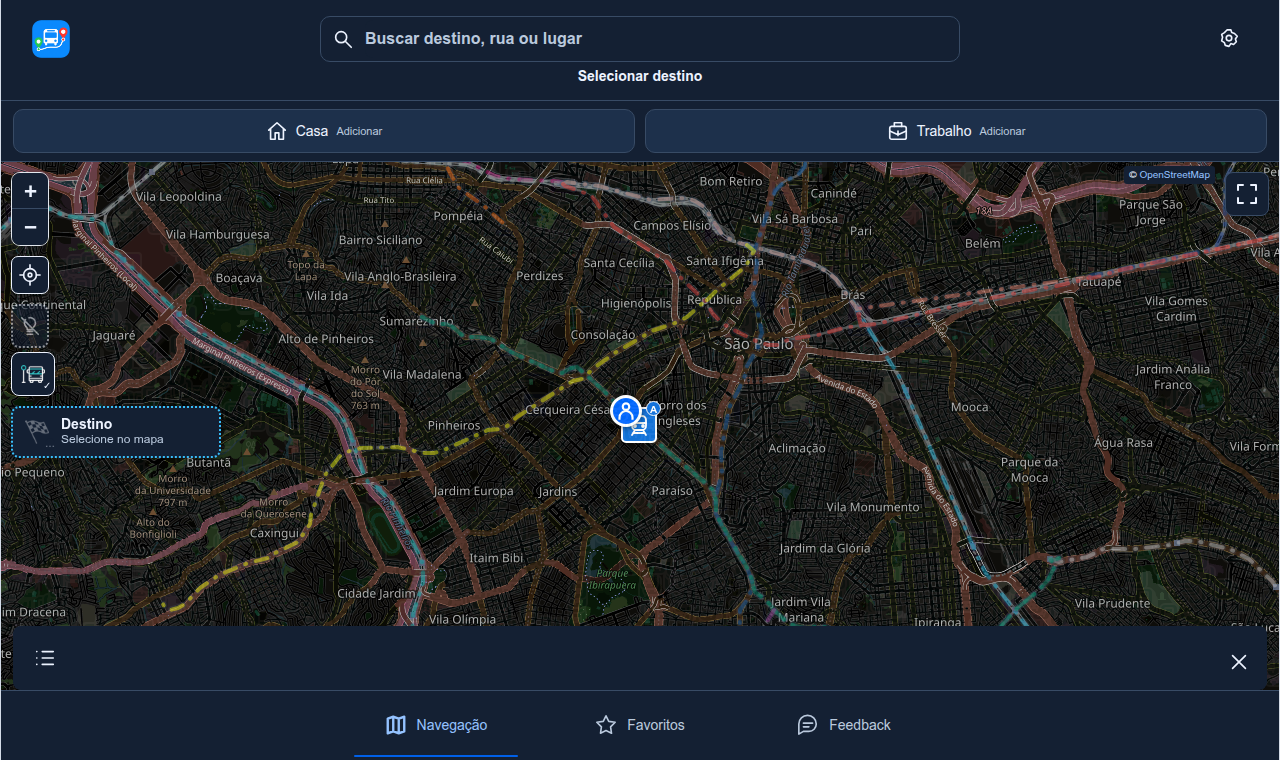
\includegraphics[width=\textwidth]{revisao-consistencia-2026-11-01/network-current.png}
\caption{Rede ferroviária e símbolos de estações antes da escolha do itinerário.}\label{fig:rede-ferroviaria-20261101}
\fonte{Captura local de 1 nov. 2026; roteiro capture\_final.cjs e hashes no manifesto da revisão.}
\end{figure}
\begin{figure}[H]
\centering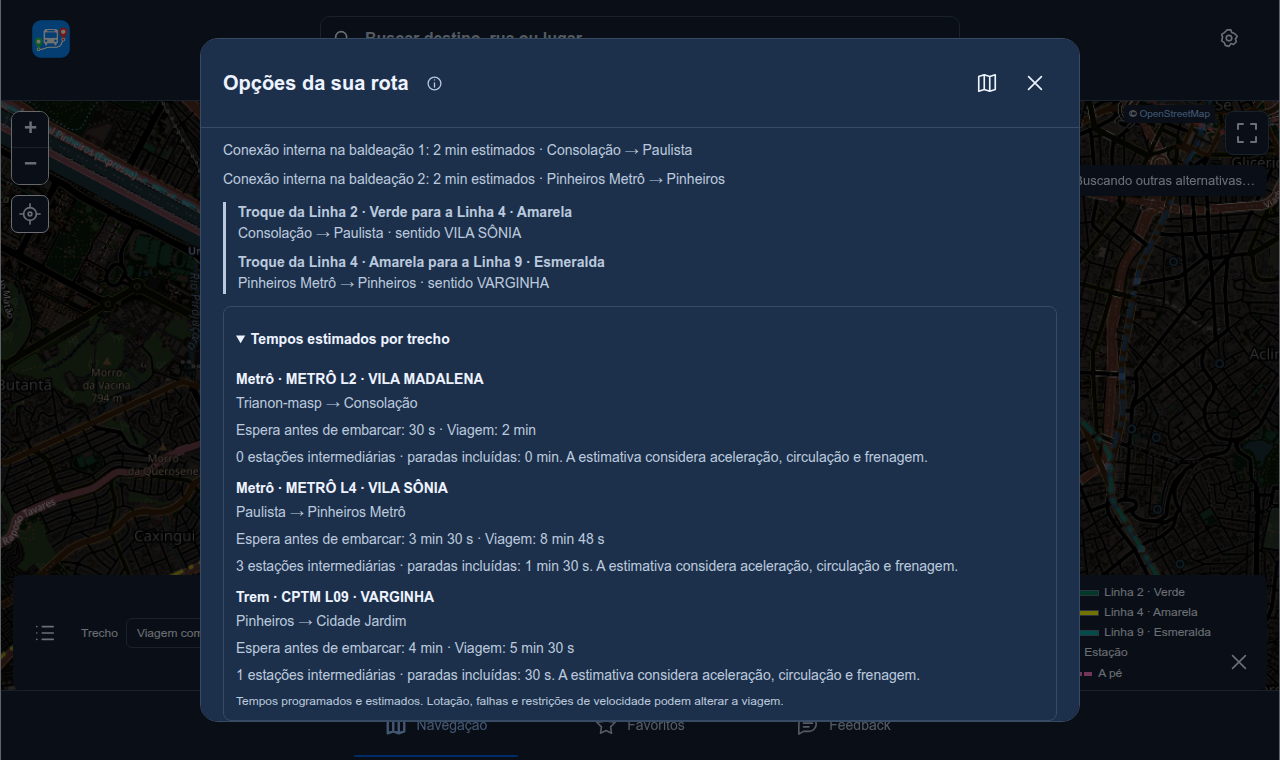
\includegraphics[width=\textwidth]{revisao-consistencia-2026-11-01/train-transfer-current.png}
\caption{Transferências Verde--Amarela--Esmeralda e decomposição das estimativas ferroviárias.}\label{fig:troca-ferroviaria-20261101}
\fonte{Mesma execução local; tempos de planejamento, sem previsão ferroviária em tempo real.}
\end{figure}

\subsection{Rastreabilidade}
As evidências estão no repositório de desenvolvimento: \nolinkurl{docs/coverage-audit-20261101.md}, \nolinkurl{docs/endpoint-audit-20261101.md}, \nolinkurl{docs/async-route-stream.md} e \nolinkurl{docs/async-performance-comparison.md}. O diretório \nolinkurl{artifacts/benchmarks/async-comparison-20261101/} preserva resultados individuais, comparação JSON, CSV pareado e validação das bases. O histórico de 28 de outubro a seguir conserva a estimativa de 226,47 GiB do desenho anterior; esse valor não corresponde ao tamanho final do banco compacto atual.


A conferência documental está em \nolinkurl{revisao-consistencia-2026-11-01/}, junto a este fonte. O CSV dos 477 casos preserva identificadores de paradas, grupos, custos e tempos, sem acessar telemetria pessoal. O manifesto retrospectivo registra hashes SHA-256 dos arquivos individuais de medição, scripts e evidências visuais, metadados dos bancos e o estado Git observado na auditoria. O HEAD de desenvolvimento observado foi \texttt{34a46f29}, com alterações locais; esse identificador sozinho não reproduz o código executado no teste. Não foi localizado no diretório do benchmark um manifesto contemporâneo completo que vincule cada execução a todos os fontes locais e à carga do equipamento.

O equipamento inspecionado nesta auditoria apresenta Intel Core i9-14900HX, 24 núcleos físicos e 32 processadores lógicos; o teste registrado utiliza 32 processos, não 32 núcleos físicos. O instrumento mantém o GTFS carregado, esvazia o cache de respostas a cada caso, recria os conjuntos de threads e aguarda o encerramento dos produtores fora do cronômetro da primeira rota. O cache do sistema operacional não foi isolado, impedindo classificar o resultado como ensaio controlado de cache frio. Os registros de execução são de 1 de novembro; 3 de novembro às 02h, 08h e 14h são instantes simulados de partida, não datas de coleta.

Os bancos foram identificados por assinatura, tamanho e data de modificação: GTFS importado em 6 de outubro, versão 2 da representação compacta e modelo ferroviário \texttt{rail-1}. As etapas-base concluídas são 0 e 1; as expansões completam vagas com limite de 8 e depois 12 unidades de um terço, preservando cinco alternativas e mínimo mais uma unidade de custo. Esses parâmetros, os limites pedestres e as assinaturas dos kernels constam do manifesto. A revisão não recalculou hash integral do banco de 88,44 GiB, não modificou dados brutos e não executou nova materialização ou benchmark. As lacunas de rastreabilidade são explicitadas, sem reconstruir retrospectivamente condições não registradas.


\section{Preparação estrutural e bancos especializados}
A construção separa dados de origem, relações estruturais e candidatos prontos para consulta. O arquivo GTFS alimenta o grafo e as ligações diretas. A malha OSM, processada pelo OSRM com perfil pedestre, fornece distâncias verificadas entre paradas; essas distâncias complementam as ligações de ônibus. O fluxo de dependências é: cadastro GTFS, grafo, conexões diretas e caminhadas, componentes reutilizáveis e, por fim, materialização seletiva. Alterações das fontes ou dos parâmetros relevantes exigem verificar as assinaturas dos derivados e reconstruir os artefatos afetados, sem refazer essa estrutura estática a cada consulta operacional.

Os seis bancos SQLite especializados têm as seguintes responsabilidades. Os nomes abaixo indicam os sufixos usados pelo conjunto de artefatos \texttt{sptrans}; não incluem o banco Django do cenário histórico de Mauá.
\begin{enumerate}
\item \textbf{Cadastro GTFS: \nolinkurl{sptrans.sqlite3}.} Persiste paradas, linhas, viagens, sequências, horários, frequências, calendários, exceções e geometrias importadas. Chaves por identificador e índices das relações entre viagens, paradas e horários sustentam as consultas. É a fonte dos demais artefatos e da programação utilizada pelos dois planejadores.
\item \textbf{Grafo: \nolinkurl{sptrans.routing.sqlite3}.} Deriva do cadastro e organiza padrões de sequência, segmentos dirigidos, calendários e dados temporais para avaliação. As chaves de padrão e sequência permitem recuperar segmentos e ocorrências de paradas. Também comporta perfis históricos por segmento, tipo de dia e faixa horária e correspondências operacionais. A existência desse esquema não significa que uma base de velocidades históricas já tenha sido preenchida ou validada.
\item \textbf{Conexões diretas: \nolinkurl{sptrans.direct.sqlite3}.} Deriva do grafo e enumera, em cada padrão, embarques e desembarques posteriores na sequência, com distâncias e referências temporais. Os índices \nolinkurl{direct_out} e \nolinkurl{direct_in} permitem acesso pela origem e pelo destino. O índice reverso consulta ligações no sentido correto de circulação; não cria uma viagem no sentido contrário.
\item \textbf{Caminhadas: \nolinkurl{sptrans.walks.sqlite3}.} Depende das paradas do grafo e da malha pedestre OSM/OSRM. Persiste ligações verificadas, distâncias de rede e acessos à malha, tempo derivado da velocidade configurada, procedência e estado de verificação. As tabelas \nolinkurl{walk_edge} e \nolinkurl{stop_snap}, com índice de entrada \nolinkurl{walk_in}, apoiam a consulta nos dois sentidos. Distância e tempo permanecem distintos. A geometria completa pode ser recuperada posteriormente para apresentação, em vez de duplicada em cada candidato.
\item \textbf{Componentes: \nolinkurl{sptrans.connections.sqlite3}.} Combina conexões diretas e caminhadas em ocorrências, ligações pedestres, transferências e saídas de ônibus seguidas de caminhada. Índices de saída, entrada e encontro permitem reutilizar componentes nas composições de um, dois ou três ônibus. As visões \nolinkurl{conexoes_1}, \nolinkurl{conexoes_2} e \nolinkurl{conexoes_3} não significam armazenamento físico de todas as combinações completas.
\item \textbf{Candidatos materializados: \nolinkurl{sptrans.materialized.sqlite3}.} Deriva dos componentes e guarda, na tabela \nolinkurl{conexoes}, referências aos trechos e caminhadas, totais de distância, tempo a pé e classificação por categoria. Índices por par, distância e sentido reverso apoiam a recuperação. O estado de materialização é registrado por par origem--destino e número de embarques, distinguindo categorias concluídas de interrupções por limite de execução. Metadados vinculam os candidatos às fontes, parâmetros e cotas usados na preparação.
\end{enumerate}

A composição bidirecional offline combina prefixos da origem com sufixos do destino, verificando encontros nas sequências dirigidas. O módulo estrutural de três ônibus reutiliza esses componentes, mas não integra o consolidado municipal atual: a versão 2 de \nolinkurl{materialized_connections.py} admite somente um ou dois ônibus, com cotas de 16 e oito candidatos por par. A cota de quatro candidatos de três ônibus permanece prevista no protocolo comparativo, não como categoria preenchida nesse banco. A seleção por distância pode excluir um percurso mais longo que seria mais rápido no horário consultado.

Em 28 de outubro de 2026, a tentativa de completar a cobertura municipal de um ou dois ônibus foi interrompida preventivamente, por solicitação do responsável, diante da incompatibilidade entre armazenamento projetado e espaço disponível no ambiente de desenvolvimento. Os registros examinados não demonstram erro por esgotamento efetivo do disco. A estimativa exploratória preservou os totais de alcançabilidade de 32 origens entre 22.011 origens de embarque. Seus identificadores correspondem a posições igualmente espaçadas, a cada 710 elementos, na lista ordenada de identificadores; esse padrão foi conferido nos dados, mas o script original da seleção não foi localizado. Não se trata de estratificação geográfica demonstrada nem de amostra probabilística. Os totais foram reproduzidos por leitura dos componentes, sem nova materialização: variam de 1.891 a 19.681 destinos por origem, com média de 7.318,03125. A média multiplicada por 22.011 resulta em 161.077.185,84375 pares, arredondados para 161.077.186. A alcançabilidade é um superconjunto estrutural que ainda pode produzir categorias vazias, não uma contagem de rotas temporalmente válidas.

O cálculo de armazenamento utiliza 117.702.656 bytes e 77.968 pares com ambas as categorias prontas, registrados naquele momento: o quociente entre esses valores, multiplicado pela projeção não arredondada de pares e dividido por $2^{30}$, reproduz 226,47 GiB. É uma extrapolação exploratória do arquivo parcial, além da qual seriam necessários arquivos temporários; não representa tamanho final medido. A distribuição de candidatos por par e o custo dos índices podem variar, e a base observada concentra as primeiras origens processadas. O registro quantitativo informa 54,15 GiB livres; a faixa de 51 a 54 GiB citada no acompanhamento não dispõe de série de medições preservada que permita reproduzir seu limite inferior. A limitação é do ambiente utilizado, sem demonstrar inviabilidade geral da abordagem.

Os 77.968 pares e 644.798 candidatos citados na estimativa são um levantamento intermediário de 28 de outubro. A leitura posterior do banco preservado, cujo último registro é de 07h50min34s desse dia, horário de Brasília, encontrou 77.988 categorias prontas de um ônibus e 77.987 de dois: 77.987 pares com ambas prontas e 644.942 candidatos (28.292 de um ônibus e 616.650 de dois). Há 77.956 pares com ao menos um candidato em categoria pronta; essa condição permite recuperação estrutural, sujeita à seleção de acessos e às validações da consulta, não comprova utilização efetiva nem viabilidade temporal. Categorias prontas podem estar vazias. A cópia \nolinkurl{materializado-antes.sqlite3} foi conferida e preserva o estado anterior à tentativa: 77.956 pares com ambas as categorias prontas e 644.702 candidatos; não é cópia do estado final. Esses levantamentos posteriores não substituem o inventário histórico de 23 de outubro da Tabela~\ref{tab:inventario-benchmark}.

O marcador \texttt{city\_complete=false} permanece: processamento por categoria, existência de candidatos, cobertura municipal, cobertura dos horários e rotas válidas são medidas distintas. Não há categoria de três ônibus no consolidado. As evidências originais estão em \nolinkurl{artifacts/materializacao-completa-2026-10-28/}, no acervo do projeto; a conferência somente de leitura, com fórmulas, hashes e limitações, está em \nolinkurl{auditoria-materializacao-2026-10-28/}, junto ao fonte deste relatório.

% TODO-BENCHMARK: Inserir tempo total da materialização.
% TODO-BENCHMARK: Inserir armazenamento final dos bancos.
% TODO-BENCHMARK: Inserir cobertura das paradas e pares.

\section{Consulta temporal e acionamento do fallback}
Com o seletor configurado para conexões e até duas baldeações, o despachante utiliza o adaptador materializado. Este recupera candidatos de um ou dois ônibus cuja respectiva categoria esteja \texttt{ready}, após validar os artefatos e selecionar paradas de acesso e saída. A recuperação parcial não exige as duas categorias prontas, uma terceira categoria ou cobertura municipal completa. As assinaturas do materializado, do índice direto e do grafo foram aceitas na conferência somente de leitura; isso não comprova sucesso de uma viagem.

A função estrita \nolinkurl{materialized_connections.query}, distinta do caminho utilizado pelo passageiro, exige ambas as categorias prontas e admite somente cotas para o conjunto $\{1,2\}$, sem consulta isolada de uma categoria. O esquema atual impede armazenar três ônibus; sua ausência não bloqueia candidatos de um ou dois.

O adaptador complementa o consolidado com o índice direto municipal e componentes de um ônibus com caminhada final. Para pares sem a categoria de dois ônibus pronta, consulta componentes de dois ônibus, limitados a oito candidatos, com prazo de cinco segundos para essa consulta estrutural. Uma categoria pronta e vazia não é recomposta. Há, portanto, composição limitada a partir dos componentes na consulta, sem materialização municipal nem gravação de novos pares. O indicador \texttt{materialized=true}, isoladamente, não comprova que todos os candidatos vieram do consolidado.

A classificação preliminar combina deslocamentos nos veículos, caminhadas e uma penalidade de referência de cinco minutos por espera intermediária. Essa penalidade serve à ordenação inicial, não substitui a espera calculada na avaliação temporal. As caminhadas de acesso, transferência e saída são validadas pelo serviço pedestre, respeitando o limite configurado. O fluxo materializado compartilha um orçamento de até 64 verificações e 30 segundos para iniciar novas verificações; os limites não asseguram que toda resposta termine em 30 segundos. Uma caminhada inválida impede publicar aquele candidato como percurso verificado.

O avaliador propaga o instante de chegada entre os trechos. Para cada embarque, consulta uma partida compatível com a chegada do passageiro, considerando caminhada e margem de transferência de 120 segundos. Calendários e exceções GTFS restringem os serviços; horários superiores a 24:00:00 preservam sua associação ao dia de serviço. A avaliação considera dias de serviço anteriores pertinentes e o seguinte, dentro do horizonte configurado de seis horas. O tempo total inclui acesso, espera inicial, permanência nos veículos, caminhadas e esperas nas transferências e saída até o destino. Distância curta, isoladamente, não assegura uma conexão temporal possível.

O mecanismo de custos admite perfis históricos de circulação por segmento, tipo de dia e faixa horária, com passagem entre faixas durante o percurso. Na ausência de um perfil completo aplicável ao segmento, utiliza o custo programado correspondente. Tempos de parada são tratados separadamente para evitar dupla contagem; velocidade comercial, que já os incorpora, não deve ser inserida como velocidade de circulação sem decomposição. Nesta revisão, não se apresenta resultado de uma base histórica preenchida. A infraestrutura de custos e a disponibilidade efetiva desses dados são estados distintos.

O refinamento com Olho Vivo exige correspondência de linha, sentido e parada e aceita previsões compatíveis com o instante de chegada ao embarque. A posição operacional não fornece automaticamente a velocidade de todos os segmentos nem um tempo exato da viagem inteira. Na indisponibilidade de previsão, permanece a avaliação programada; essa ocorrência isolada não aciona o planejador por rodadas. O orçamento operacional limita as consultas externas, sem reconstruir os artefatos estáticos. As alternativas válidas são reordenadas e enviadas progressivamente, retendo até cinco resultados distintos na configuração de referência. A duração continua sendo estimada e sua ordem pode mudar durante o processamento.

No fluxo de ônibus, o despachante aciona a busca por rodadas quando a preparação não oferece contexto utilizável ou informa indisponibilidade, ou quando a avaliação das conexões termina sem alternativas. A ausência ou incompatibilidade do consolidado pode ser suprida pelas consultas aos outros índices; não determina, sozinha, o fallback. O adaptador avalia no máximo dois ônibus mesmo quando a solicitação admite três; o terceiro depende do caminho por rodadas. Se a avaliação de conexões termina com alternativas, não há busca adicional de três ônibus para completar a lista. A seleção explícita de rodadas ou profundidade fora do limite de entrada do adaptador conduz ao caminho alternativo, quando permitido. Na configuração atual, uma caminhada direta já validada com menos de 1.000 m desabilita essa tentativa por rodadas. Além disso, os filtros posteriores de apresentação podem remover alternativas sem reabrir o fallback. Não se afirma recuperação automática de qualquer erro de programação.

Os dois planejadores não são executados simultaneamente nem têm seus resultados obrigatoriamente unidos. O identificador do produtor acompanha o retorno; o retorno de fallback pode conservar a razão de indisponibilidade ou apresentar uma mensagem genérica. Para os benchmarks, será necessário registrar motivos discriminados no instrumento de medição, sem deduzi-los apenas dessa mensagem. As cotas por distância, os limites de validação e o filtro de alternativas distintas não constituem uma fronteira de Pareto completa. As regras de poda por chegada descritas a seguir pertencem ao planejador por rodadas; não se atribui à consulta materializada uma poda global pelo melhor tempo que ela não executa.

\section{Protocolo do benchmark definitivo}\label{sec:benchmark-hibrido}
O protocolo será executado após a conclusão e verificação da materialização. A configuração A do estudo principal é o caminho completo de conexões, sem fallback: consolidado materializado, índice direto, componentes auxiliares e composição estrutural limitada na consulta, conforme B.2. Inclui as validações pedestres e temporais e o refinamento operacional, mantendo como vazio um resultado sem alternativas válidas. Permanecem B, planejador por rodadas isolado, e C, arquitetura integrada com fallback. Cada resultado deverá identificar o mecanismo que efetivamente o produziu. Uma consulta estrita apenas aos candidatos previamente materializados, se investigada, será uma análise auxiliar distinta de A. O plano não constitui resultado experimental.

Antes da coleta, o instrumento deverá registrar separadamente a procedência dos candidatos: consolidado materializado por categoria, índice direto, componentes de um ônibus e componentes de dois ônibus. Quando houver deduplicação, deverá preservar todas as origens de um mesmo candidato e distinguir quantidades recuperadas, avaliadas e válidas. O indicador genérico \texttt{materialized=true} não substitui esse registro; essa instrumentação é requisito do estudo proposto, não uma coleta já concluída.

O consolidado e o caminho de conexões atuais atendem somente a um ou dois ônibus. Esse será o limite comum da comparação principal A/B/C, inclusive nas rodadas do fallback. Comparações com três embarques dependem dessa capacidade em A e nas demais configurações, sob condições equivalentes de consulta e validação. Enquanto isso, A não equivale a buscas por rodadas que admitam três ônibus.

As três configurações utilizarão os mesmos pares origem--destino, instantes de partida e fuso, pacote e calendários GTFS, velocidade de caminhada de 4,5 km/h, limites de distância, número máximo de embarques, critérios temporais e informações operacionais. O instrumento deverá equalizar também o tratamento de caminhadas iniciais e finais e o refinamento temporal; apenas aplicar os parâmetros aos fluxos existentes não comprova equivalência. Serão registrados a revisão do código, eventuais alterações locais, assinaturas dos bancos, configuração, hardware e versões dos serviços. A amostra deverá incluir viagens diretas, baldeações, caminhadas de acesso e saída, períodos diurnos e noturnos e casos sem rota. Selecionar somente pares com sucesso no materializado impediria medir sua cobertura e a necessidade do fallback.

\textbf{Teste controlado.} As respostas operacionais e pedestres serão congeladas e reutilizadas. As consultas serão repetidas em execuções isoladas, alternando a ordem dos planejadores. Serão separadas condições de cache frio e quente, documentando quais caches foram reiniciados ou preservados, inclusive os do sistema operacional. O número de repetições e a amostra serão definidos antes da coleta; percentis extremos exigem quantidade suficiente de observações. Serão medidos latência até a primeira alternativa e até o término, memória e atividade de preparação separadamente. A materialização e outros trabalhos intensivos não deverão competir com as consultas medidas.

\textbf{Teste operacional.} Os planejadores serão consultados sequencialmente em instantes próximos, com dados atuais da SPTrans, alternando sua ordem e registrando os instantes de requisição e das informações retornadas. A comparação examinará viabilidade dos embarques, alternativas e sensibilidade à atualização dos dados. Respostas diferentes entre duas consultas serão explicitadas, não tratadas como se fossem a mesma observação congelada. Eventual concorrência por recursos ou variação da rede não será interpretada como diferença intrínseca entre algoritmos.

% TODO-BENCHMARK: Inserir latências até a primeira alternativa e até o término, por configuração e cache.
% TODO-BENCHMARK: Inserir qualidade dos itinerários, viabilidade e diferenças temporais.
% TODO-BENCHMARK: Inserir frequência, motivos e custo do fallback no fluxo integrado.
% TODO-BENCHMARK: Inserir comparação A (conexões sem fallback), B (rodadas) e C (integrado), com amostra e limites.
\textbf{Métricas e critérios de análise.} Para cada configuração e condição de cache, registrar latências p50, p95 e p99, média, desvio-padrão e tamanho da amostra; quantidade de candidatos examinados e alternativas temporalmente válidas; melhor duração, baldeações, caminhada e espera, incluindo sua decomposição por etapa. Registrar consumo de memória, tamanho final de cada banco e do conjunto e tempo total de preparação, discriminando suas etapas. No fluxo integrado, medir frequência e motivos de fallback, tempo consumido antes de seu acionamento e produtor de cada resposta.

A qualidade será comparada por cobertura, compatibilidade temporal e diferença entre as melhores durações encontradas, sem assumir que um dos planejadores limitados fornece o ótimo global. Deverá ser examinada a perda causada pelas cotas efetivas de 16 e oito candidatos, mediante amostras com cotas ampliadas ou referência independente, quando viável. A cota de quatro para três ônibus permanece como investigação futura, condicionada à capacidade e à equivalência de escopo descritas acima. Resultados sem rota serão contabilizados e terão suas causas distinguidas de timeout e falha externa. A conclusão sobre o compromisso entre preparação, armazenamento, latência e alternativas somente será redigida após essas medições.


\textbf{Comparabilidade das alternativas.} Para não confundir igualdade de representação com utilidade equivalente, o protocolo distinguirá: itinerários com a mesma sequência dirigida de linhas, paradas e ocorrências de embarque; o mesmo deslocamento com variações nos acessos a pé; itinerários distintos com chegada temporalmente equivalente; alternativa mais rápida encontrada por apenas um mecanismo; alternativa inviável; e ausência de resultado. A tolerância temporal e o critério para agrupar variações de caminhada deverão ser definidos antes da coleta, com preservação dos valores exatos de chegada, distância, espera e baldeações. Uma alternativa inviável não será classificada como equivalente por apresentar duração semelhante. Essa classificação complementa as métricas de cobertura e latência, sem alterar as três configurações comparadas ou antecipar resultados.

\section{Situação dos benchmarks em 23 de outubro de 2026}
A revisão dos artefatos disponíveis não localizou uma nova execução do benchmark definitivo. Os resultados encontrados nos diretórios de evidências datam de 7 e 8 de outubro e não foram promovidos a resultados finais. Foi realizado um inventário somente de leitura dos seis bancos utilizados pela aplicação, com registro de tamanho e SHA-256. O script e os dados brutos estão em \nolinkurl{benchmarks/2026-10-23/}. Trata-se de diagnóstico de preparação, não de comparação experimental dos planejadores.

\begin{table}[H]\centering
\caption{Armazenamento observado em 23 de outubro, antes da conclusão da materialização.}\label{tab:inventario-benchmark}
\begin{tabular}{lr}\hline
Arquivo & Tamanho (MiB)\\\hline
\nolinkurl{sptrans.sqlite3} & 70,04\\
\nolinkurl{sptrans.routing.sqlite3} & 595,36\\
\nolinkurl{sptrans.direct.sqlite3} & 402,20\\
\nolinkurl{sptrans.walks.sqlite3} & 446,32\\
\nolinkurl{sptrans.connections.sqlite3} & 2907,56\\
\nolinkurl{sptrans.materialized.sqlite3} & 112,23\\
\hline
Total & 4533,70\\\hline
\end{tabular}
\fonte{Inventário local somente de leitura; 1 MiB = 1.048.576 bytes.}
\end{table}

Os valores representam o tamanho lógico dos arquivos principais naquele instante, sem incluir eventuais arquivos auxiliares, caches ou exportações; não representam armazenamento final da materialização municipal. As assinaturas permaneceram estáveis quanto ao tamanho e à data de modificação durante a leitura de cada arquivo, sem constituir um snapshot transacional conjunto.

O banco materializado informa \texttt{city\_complete=false}. Seu catálogo contém 77.957 pares na categoria de um ônibus e 77.956 na categoria de dois ônibus, todos marcados como \texttt{ready}; 77.956 pares possuem ambas as categorias. Há 644.702 candidatos armazenados. O esquema desse artefato admite apenas essas duas categorias, não a categoria de três ônibus prevista no protocolo. O estado \texttt{ready} indica processamento da categoria, inclusive quando ela não produz caminho: as contagens não equivalem a cobertura de viagens viáveis. Os validadores existentes aceitaram as assinaturas dos componentes e do materializado, o que não comprova conclusão municipal nem equivalência das três configurações experimentais.

Permanecem sem medição definitiva o tempo total de preparação, a latência até a primeira alternativa e até o término, a cobertura temporal, a qualidade dos itinerários e a frequência e o custo de fallback. Não foram calculados percentis com base nos registros históricos nem somados tempos parciais como se representassem o tempo total de preparação. A comparação A/B/C deverá ocorrer após conclusão e verificação da materialização, com amostra, repetições, tolerâncias e condições de cache definidas previamente, conforme o protocolo preservado. Nenhuma materialização ou consulta comparativa foi iniciada nesta revisão.



\section{Representação e composição do custo}
Paradas representam locais de embarque e desembarque. A sequência de paradas de uma viagem e seus horários determinam conexões dirigidas: estar perto de uma linha não significa poder embarcar no sentido desejado. Calendários e janelas de operação restringem as partidas utilizáveis. Ligações a pé permitem acessar outra parada na origem, realizar uma transferência ou alcançar o destino após o desembarque. Essa combinação exige considerar o tempo em que cada conexão pode ser utilizada, como discutem \citet{bast2015}.

Para uma partida da consulta em $t_0$, a comparação usa a chegada estimada ao destino, incluindo caminhada, espera e deslocamento nos veículos. A duração de uma caminhada de distância $d$, em metros, é calculada por $t_p(d)=60d/4500$, em minutos, adotando 4,5 km/h na configuração atual. A distância permanece armazenada separadamente; o tempo a essa velocidade pode ser persistido para reutilização. A revisão histórica descrita anteriormente adotava 4 km/h, diferença que deve ser eliminada na preparação de comparações equivalentes. O limite é de 1 km por percurso a pé de acesso, transferência ou saída; a soma das caminhadas da viagem pode superar esse valor. A velocidade e os limites são parâmetros do protótipo, não resultados de medição com passageiros. O valor de 1 km não representa uma distância considerada adequada para todos os passageiros. O planejamento reserva 120 segundos para a troca de veículo e trabalha com horizonte de seis horas. Quando os dados descrevem frequência sem horário exato, utiliza uma estimativa de espera de metade do intervalo; isso não identifica a posição efetiva do ônibus.

\section{Dijkstra, A* e busca por rodadas}
Dijkstra fundamenta a busca de caminhos mínimos com custos não negativos \citep{dijkstra1959}. No cenário demonstrativo de Mauá, esse princípio apoia o planejamento com os tempos disponibilizados. O A* combina custo acumulado e uma estimativa do custo restante \citep{hart1968}. No procedimento histórico de geolocalização de Mauá, ele operava sobre conexões viárias e distâncias; não previa duração de viagens de passageiros. Essa etapa foi dispensada no cenário São Paulo pela adoção das coordenadas GTFS, conforme o Apêndice~\ref{ap:importacao}.

No mecanismo alternativo do cenário São Paulo, o planejador processa rodadas correspondentes a novos embarques. Cada rodada parte dos estados da anterior, evitando utilizar uma transferência descoberta para embarcar novamente na mesma rodada. A configuração padrão permite dois transbordos, isto é, até três embarques. Essa organização se relaciona à programação dinâmica por rodadas do RAPTOR \citep{delling2012}. O código do PaP é uma implementação própria e limitada; não se atribuem a ele todas as propriedades, desempenho ou variantes multicritério do RAPTOR.

A inicialização considera simultaneamente as paradas candidatas de origem, acrescentando seus tempos de acesso. A avaliação final considera as paradas candidatas de desembarque e o tempo de caminhada restante. Assim, o menor tempo depende da chegada ao destino, e não apenas da proximidade da parada. Descer antes pode vencer uma volta longa do veículo, desde que haja percurso a pé admissível; permanecer a bordo pode vencer quando a economia de caminhada superar o tempo adicional no ônibus.

\section{Dominância, poda e encerramento}
No planejador por rodadas, um estado registra uma chegada a uma parada e os trechos que a produziram. Mantidas as possibilidades de continuação do modelo, uma chegada posterior não melhora uma chegada anterior ao mesmo estado. A busca atualiza os melhores tempos conhecidos e usa uma chegada completa ao destino como limite superior. Como os custos seguintes são não negativos, um estado cujo tempo já atinge esse limite não pode produzir uma chegada estritamente melhor. A comparação temporal inclui a caminhada final; podar por distância isolada seria inadequado.

A apresentação também remove uma alternativa com embarques adicionais quando outra utiliza o mesmo prefixo de linhas, chega no mesmo horário ou antes e exige caminhada igual ou menor. Esse filtro evita apresentar uma baldeação extra dominada; não elimina toda transferência curta, pois ela pode ser necessária em outros contextos.

Essa regra serve ao objetivo de melhor chegada. Descartar empates ou alternativas dominadas não preserva necessariamente todas as sequências de linhas possíveis. Por isso, a lista de alternativas calculadas não deve ser descrita como enumeração exaustiva dos caminhos nem como garantia das melhores rotas distintas de toda a rede. A busca termina quando não há estados úteis ou quando atinge o limite de embarques, em vez de continuar expandindo sequências indefinidamente.

\section{Validação das caminhadas e retorno progressivo}
No planejador por rodadas, a proximidade geográfica fornece candidatos e uma estimativa inicial otimista de caminhada. Os percursos envolvidos nas alternativas promissoras são consultados no serviço de roteamento a pé. Uma ligação acima do limite ou sem verificação válida é retirada das opções; uma distância corrigida altera os custos e provoca nova busca. Uma linha reta entre coordenadas não é publicada como caminhada verificada. O método reduz consultas externas, mas seu resultado depende da disponibilidade e da qualidade da malha usada pelo serviço.

Nesse mecanismo alternativo, o ciclo de validação admite até 12 rodadas, 32 verificações de caminhadas de transferência e 64 verificações de caminhada ao todo. O limite de 30 segundos impede iniciar novas consultas após esse prazo; não é um prazo rígido para toda a resposta, pois uma consulta em andamento pode terminar depois. Ao atingir os limites, o processamento final utiliza conexões já verificadas e informa a limitação. Resultados são enviados progressivamente, de modo que a primeira alternativa apresentada não é necessariamente a mais rápida. A ordem pode melhorar conforme os percursos são validados.


\begin{figure}[H]
\centering\begin{tikzpicture}[>=Stealth,font=\small,stop/.style={circle,draw,minimum size=9mm}]
\node[stop] (a) at (0,0) {A};\node[stop] (b) at (4,0) {B};\node[stop] (c) at (8,0) {C};\node[stop] (d) at (4,-3) {D};
\draw[->,very thick,blue!70!black] (a)--node[above]{ônibus: 8 min}(b);
\draw[->,thick] (b)--node[above]{ônibus: 12 min}(c);
\draw[->,dashed,very thick,blue!70!black] (b)--node[left,align=right]{a pé: 400 m\\5 min 20 s}(d);
\draw[->,dashed,gray] (c)--node[below right,align=left,text=black]{a pé: 200 m\\2 min 40 s}(d);
\node[draw,fill=blue!5,align=center,text width=5.2cm] at (1,-4.6) {A $\to$ B $\to$ D = 13 min 20 s\\Melhor chegada conhecida};
\node[draw,align=center,text width=5.2cm] at (7.4,-4.6) {A $\to$ B $\to$ C $\to$ D\\= 22 min 40 s; descartada};
\node[draw,fill=black!5,align=center] at (4,-6) {C é alcançado em 20 min $\geq$ 13 min 20 s.\\Podar sua expansão: custos seguintes não negativos.};
\end{tikzpicture}

\caption{Exemplo didático de desembarque antecipado e poda temporal.}\label{fig:grafo-poda}
\fonte{Elaboração do grupo; exemplo atualizado para caminhada a 4,5 km/h em 22 out. 2026.}
\end{figure}

No exemplo da Figura~\ref{fig:grafo-poda}, D é o destino final e todos os custos são ilustrativos. A espera inicial é igual nas duas alternativas e foi omitida. As conexões a pé pressupõem percursos verificados; o exemplo não representa coordenadas ou uma linha real.

\section{Alcance dos resultados e reprodução}
O indicador interno de melhor resultado dentro dos limites deve ser interpretado no domínio do modelo: cadastro importado, horário de consulta, profundidade permitida, custos estimados e conexões a pé verificadas. Não equivale a uma garantia sobre trânsito, acessibilidade física ou operação real. Interrupções de serviço ou esgotamento do orçamento de validação restringem ainda mais essa interpretação.

Uma comparação reproduzível deve conservar versão do código, arquivo GTFS, instante e fuso da consulta, origem, destino, limites e respostas do serviço de caminhada. O exemplo didático de duas alternativas ilustra o critério: se permanecer no ônibus exige mais 12 minutos e descer em uma parada anterior permite caminhar 400 m, essa caminhada corresponde a 5 minutos e 20 segundos a 4,5 km/h. Na Figura~\ref{fig:grafo-poda}, desembarcar em B resulta em 13 minutos e 20 segundos; seguir até C e caminhar mais 200 m resulta em 22 minutos e 40 segundos. A diferença é de 9 minutos e 20 segundos, considerando todos os custos representados. Esses números são ilustrativos, não uma medição operacional.

% Conteúdo independente para a revisão estilística v2: engenharia_apendice
\chapter{Documentação de engenharia de software do PaP}\label{ap:engenharia}
Os diagramas desta revisão documentam retrospectivamente a extensão São Paulo. A notação é simplificada, baseada nas perspectivas de casos de uso, sequência e estados da UML \citep{uml251}. Os nomes dos estados são conceituais; não são uma transcrição de variáveis da implementação. A separação mantém no corpo a visão geral e reserva aqui os detalhes de comportamento.
\section{Atores e casos de uso}
O passageiro utiliza a consulta de transporte sem cadastro obrigatório e pode escolher ou interromper sua participação na pesquisa, enviar feedback voluntário e solicitar exclusão de dados. O administrador representa tanto a operação técnica do cadastro quanto a gestão restrita dos registros de pesquisa. A importação por comando não implica existência de um botão na interface do passageiro.

Na revisão \texttt{85417bc}, a administração permite consultar sessões, metadados, eventos e reprodução da navegação, exportar registros em JSON ou vídeo WebM e excluir sessões com confirmação. O replay reconstrói eventos registrados com rrweb; não equivale a filmagem contínua, e a exportação não contém áudio. Sua fidelidade depende dos eventos recebidos e das imagens disponíveis. Em atualização de 25 de outubro de 2026, o grupo informou a conclusão e a verificação do replay. Essa confirmação não equivale a um novo ensaio independente documentado neste relatório.

O painel de pesquisa permite consultar feedback e solicitações, marcar mensagens como analisadas e excluí-las com confirmação. Novas mensagens são armazenadas separadamente da telemetria: um relato sem gravação ativa não cria sessão nem replay. Com sessão ativa, o relato também pode ser apresentado no detalhe da sessão. Excluir uma sessão não elimina essas mensagens independentes; marcar uma solicitação como analisada tampouco executa a exclusão solicitada. A equipe deve tratar separadamente mensagens, registros e cópias baixadas.

Os painéis exigem usuário administrativo ativo, com permissão \texttt{is\_staff}, e ficam bloqueados na instância pública. A Figura~\ref{fig:casos-pap} agrupa as responsabilidades por ator; não representa a concessão dessas funções ao passageiro nem a criação de dois sistemas independentes.

\begin{figure}[H]
\centering\resizebox{\textwidth}{!}{\begin{tikzpicture}[font=\fontsize{8}{10}\selectfont,
uc/.style={draw,ellipse,align=center,text width=3.5cm,minimum height=.8cm},
actor/.pic={\draw (0,.45) circle (.15);\draw (0,.3)--(0,-.25);\draw (-.3,.08)--(.3,.08);\draw (0,-.25)--(-.3,-.6);\draw (0,-.25)--(.3,-.6);}]
\draw (1,-9.6) rectangle (6.3,1);
\draw (8.9,-9.6) rectangle (14.2,1);
\node[font=\bfseries] at (3.65,.65) {PaP: passageiro};
\node[font=\bfseries] at (11.55,.65) {PaP: administração};
\pic at (0,-3.5) {actor};\node[rotate=90] at (-.65,-3.5) {Passageiro};
\pic at (7.9,-3.5) {actor};\node[rotate=90] at (7.25,-3.5) {Administrador};
\node[uc] (u00) at (3.65,-0.35) {Identificar embarque e\\consultar próximos ônibus};
\draw (0.35,-3.5)--(u00.west);
\node[uc] (u01) at (3.65,-1.9500000000000002) {Planejar por destino e\\ver rota e trechos};
\draw (0.35,-3.5)--(u01.west);
\node[uc] (u02) at (3.65,-3.5500000000000003) {Gerenciar favoritos};
\draw (0.35,-3.5)--(u02.west);
\node[uc] (u03) at (3.65,-5.15) {Escolher ou interromper\\participação na pesquisa};
\draw (0.35,-3.5)--(u03.west);
\node[uc] (u04) at (3.65,-6.75) {Enviar feedback\\voluntário};
\draw (0.35,-3.5)--(u04.west);
\node[uc] (u05) at (3.65,-8.35) {Solicitar exclusão\\dos dados de pesquisa};
\draw (0.35,-3.5)--(u05.west);
\node[uc] (u10) at (11.55,-0.35) {Importar e consultar\\cadastro de transporte};
\draw (8.25,-3.5)--(u10.west);
\node[uc] (u11) at (11.55,-1.9500000000000002) {Consultar sessões,\\eventos e replay};
\draw (8.25,-3.5)--(u11.west);
\node[uc] (u12) at (11.55,-3.5500000000000003) {Exportar registros JSON\\e vídeo WebM};
\draw (8.25,-3.5)--(u12.west);
\node[uc] (u13) at (11.55,-5.15) {Excluir sessão\\e suas exportações};
\draw (8.25,-3.5)--(u13.west);
\node[uc] (u14) at (11.55,-6.75) {Consultar feedback e\\solicitações de pesquisa};
\draw (8.25,-3.5)--(u14.west);
\node[uc] (u15) at (11.55,-8.35) {Marcar mensagens como\\analisadas ou excluí-las};
\draw (8.25,-3.5)--(u15.west);
\end{tikzpicture}
}
\caption{Atores e principais casos de uso do PaP.}\label{fig:casos-pap}
\fonte{Elaboração do grupo; diagrama revisado em 25 out. 2026, com base na revisão 85417bc.}
\end{figure}

\section{Consulta progressiva de alternativas}
A Figura~\ref{fig:sequencia-pap} representa o fluxo multimodal concorrente inspecionado em 1 de novembro de 2026. A consulta pode publicar primeiro uma caminhada curta já materializada. Em seguida, fontes independentes avaliam candidatos preparados e buscas complementares. A busca por rodadas depende de habilitação: uma caminhada direta válida inferior a 1 km a dispensa. A busca externa de caminhada só é criada se não houver caminhada direta inicial. O produtor de conexões de ônibus depende da configuração e da disponibilidade de seu contexto; portanto, criar uma tarefa não significa obter candidatos. Sem base utilizável, permanece o caminho alternativo previsto no código. A primeira alternativa aprovada pelos filtros é publicada sem aguardar todas as fontes, e outras podem chegar posteriormente. Validação temporal, caminhada verificável e limites continuam necessários. O fluxo sequencial anterior está preservado como registro histórico na Seção~\ref{sec:historico-arquitetura} e na cópia do diagrama anterior que acompanha a revisão documental; não descreve a execução multimodal atual.

\begin{figure}[H]
\centering\begin{tikzpicture}[>=Stealth,font=\small,
seqstage/.style={draw,rounded corners=3pt,align=left,text width=12cm,inner sep=9pt,fill=blue!3},
arr/.style={->,thick},note/.style={align=left,text width=12cm,font=\footnotesize}]
\node[seqstage] (a) at (0,0) {\textbf{1. Receber a consulta}\\A interface React envia origem, destino e instante ao backend Django.};
\node[seqstage,below=.4cm of a] (b) {\textbf{2. Recuperar candidatos}\\Django consulta o consolidado materializado, o índice direto e componentes auxiliares. A composição online limita-se a até dois ônibus, com cotas e prazos. Se o contexto estiver indisponível ou incompatível, segue para a condição da etapa 6.};
\node[seqstage,below=.4cm of b] (c) {\textbf{3. Validar e avaliar cada candidato}\\O serviço pedestre verifica as caminhadas. Django avalia os tempos e descarta alternativas incompatíveis.};
\node[seqstage,below=.4cm of c] (d) {\textbf{4. Refinar com dados operacionais, quando disponíveis}\\A API Olho Vivo fornece previsões compatíveis. Sem previsão utilizável, mantém-se a informação programada.};
\node[seqstage,fill=green!6,below=.4cm of d] (e) {\textbf{5. Mostrar alternativas conforme ficam disponíveis}\\Django envia resultados progressivamente à interface (NDJSON). As etapas 3 a 5 se repetem dentro dos limites da consulta.};
\foreach \a/\b in {a/b,b/c,c/d,d/e}{\draw[arr] (\a.south)--(\b.north);}
\node[seqstage,fill=orange!8,below=1.5cm of e] (f) {\textbf{6. Usar o planejador por rodadas somente se necessário}\\Acionar se as rodadas forem permitidas e ocorrer uma das situações:\\• contexto inutilizável na etapa 2; ou\\• término do caminho principal sem alternativas válidas.\\Os resultados do fallback também são enviados à interface.};
\node[note,anchor=north,yshift=-.2cm] at (e.south) {\textbf{Ao terminar:} se há alternativa válida, concluir sem rodadas.\\Se não há, verificar as condições abaixo.};
\node[note,below=.35cm of f] {\textbf{Regras de leitura:} não há execução simultânea dos dois planejadores. O fallback não serve para completar uma lista válida. A ausência isolada de previsão não o aciona. Caminhada direta validada inferior a 1 km dispensa rodadas.};
\end{tikzpicture}

\caption{Consulta multimodal: produtores concorrentes e publicação progressiva.}\label{fig:sequencia-pap}
\fonte{Elaboração do grupo; inspeção de alternatives.py e concurrent\_sources.py em 1 nov. 2026.}
\end{figure}

\section{Estados da navegação}
Cancelar a confirmação mantém a tela anterior; confirmar remove o trajeto, o embarque e o destino e retorna à seleção de embarque, preservando os favoritos e o enquadramento do mapa. A confirmação pode ser aberta tanto pela lista quanto pelo mapa. A visualização e o andamento do cálculo são dimensões distintas. Com localização conhecida, o fluxo inicia na seleção de destino. Alterar o embarque preserva o destino e aceita parada ou coordenada por toque prolongado. Uma falha de atualização não deve ser interpretada como cancelamento pelo usuário. Sem alternativa disponível, a interface permite revisar a consulta; as transições de recuperação complementam o caminho principal ilustrado.

\begin{figure}[H]
\centering\begin{tikzpicture}[>=Stealth,font=\small,box/.style={draw,rounded corners,align=center,text width=3.7cm,minimum height=.85cm,fill=black!3},arr/.style={->,thick,rounded corners=2pt},lab/.style={font=\scriptsize,fill=white,align=center,inner sep=2pt}]
\node[circle,fill,minimum size=2.5mm,inner sep=0pt] (start) at (0,1.3) {};
\node[box] (a) at (0,0) {Selecionando embarque};
\node[box] (b) at (6,0) {Consultando próximos ônibus};
\node[box] (c) at (0,-2.6) {Selecionando destino};
\node[box] (e) at (0,-4.4) {Consultando alternativas};
\node[box] (f) at (0,-6.2) {Visualizando rota no mapa};
\node[box] (conf) at (6,-6.2) {Confirmando cancelamento};
\draw[arr] (start.south)--(a.north);
\draw[arr] (start.west)--(-3,1.3)--(-3,-2.35)--([yshift=2.5mm]c.west);
\node[lab,text width=1.9cm] at (-3,-1.2) {localização\\conhecida};
\draw[arr] (a)--node[lab,above]{QR Code\\ou link}(b);
\draw[arr] (a.south)--node[lab,left,pos=.35]{embarque\\no mapa}(c.north);
\draw[arr] (b.south)--(6,-1.7)--node[lab,above]{selecionar destino}(1,-1.7)--([xshift=1cm]c.north);
\draw[arr] (c)--node[lab,right]{destino definido}(e);
\draw[arr] ([xshift=7pt]e.south)--node[lab,right]{selecionar rota}([xshift=7pt]f.north);
\draw[arr] ([xshift=-7pt]f.north)--node[lab,left]{reabrir lista}([xshift=-7pt]e.south);
\draw[arr] ([yshift=6pt]f.east)--node[lab,above]{cancelar}([yshift=6pt]conf.west);
\draw[arr] ([yshift=-6pt]conf.west)--node[lab,below]{continuar}([yshift=-6pt]f.east);
\draw[arr] (conf.east)--(8.3,-6.2)--(8.3,2)--(1,2)--([xshift=1cm]a.north);
\node[lab,text width=2.3cm] at (8.3,-3.3) {confirmar:\\desmarcar embarque\\e destino};
\draw[arr] ([yshift=-2.5mm]c.west)--(-4.4,-2.85)--(-4.4,0)--(a.west);
\node[lab,text width=1.1cm] at (-4.4,-.9) {sem\\origem};
\draw[arr] (f.south)--(0,-7.3)--(-5.2,-7.3)--(-5.2,2.7)--(-1,2.7)--([xshift=-1cm]a.north);
\node[lab,text width=2.3cm] at (-5.2,-4.7) {alterar\\embarque:\\preservar destino};
\node[align=center,text width=13cm,font=\scriptsize] at (1.2,-8.5) {A confirmação também pode ser aberta na lista. Continuar mantém a visualização anterior;\\confirmar preserva os favoritos e o enquadramento do mapa.};
\end{tikzpicture}

\caption{Estados conceituais da navegação e confirmação de cancelamento.}\label{fig:estados-pap}
\fonte{Elaboração do grupo; diagrama revisado em 22 out. 2026.}
\end{figure}

\section{Rastreabilidade e evidências}
% Compactação local: manter tabela e evidências na mesma página.
\begingroup
\setlength{\parskip}{4pt}
A~Tabela~\ref{tab:rastreabilidade} relaciona requisitos, responsabilidades e verificações localizadas no código. A tabela identifica testes no código; suas execuções são documentadas separadamente, com as respectivas datas e versões.
\begingroup\small\SingleSpacing\setlength{\parskip}{0pt}\setlength{\LTpre}{3pt}\setlength{\LTpost}{0pt}\setlength{\LTcapwidth}{\textwidth}
\begin{longtable}{>{\raggedright\arraybackslash}p{1.2cm}>{\raggedright\arraybackslash}p{3cm}>{\raggedright\arraybackslash}p{6cm}>{\raggedright\arraybackslash}p{3.1cm}}
\caption{Rastreabilidade dos requisitos e limites das evidências.}\label{tab:rastreabilidade}\\
\hline ID & Responsabilidade & Verificação identificada / proposta & Limite\\\hline\noalign{\vskip 1pt}\endfirsthead
\hline ID & Responsabilidade & Verificação identificada / proposta & Limite\\\hline\noalign{\vskip 1pt}\endhead
RF01 & Entrada e seleção do ponto & Testes de embarque; completar roteiro de leitura de QR Code em dispositivo físico & Não prova implantação no ponto\\ \noalign{\vskip 1pt}
RF02 & Consulta de partidas & Testes backend em \mbox{\small\texttt{test\_sptrans.py}}; inspecionar aviso da fonte & Disponibilidade real varia\\ \noalign{\vskip 1pt}
RF03 & Planejador e caminhada & \mbox{\small\texttt{test\_sptrans\_planner.py}} e \mbox{\small\texttt{test\_sptrans\_walking.py}} & Cenários controlados, não validação de toda a rede\\ \noalign{\vskip 1pt}
RF04 & Mapa e lista & Testes E2E de seleção de trecho, baldeações B/C e caminhada final & Compreensão depende de avaliação\\ \noalign{\vskip 1pt}
RF05 & Favoritos locais & Testes E2E de nome persistido, edição e confirmação de remoção & Armazenamento depende do navegador\\ \noalign{\vskip 1pt}
RF06 & Diálogo de cancelamento & Teste E2E de cancelamento confirmado & Não mede erros reais de uso\\ \noalign{\vskip 1pt}
RF07 & Rastreamento e previsão & \mbox{\small\texttt{test\_sptrans\_tracking.py}}, \mbox{\small\texttt{live-bus.spec.js}} e \mbox{\small\texttt{boardingTime.test.js}} & Não mede precisão da operação real\\ \noalign{\vskip 1pt}
RQ01 & Estado da interface e resposta progressiva & Testes E2E de stream, preservação da escolha e atualização sem redefinir mapa & Não mede tempo em toda condição de rede\\ \noalign{\vskip 1pt}
RQ02 & Fluxo de interação & Protocolo por tarefas descrito na metodologia & Avaliação com passageiros pendente\\ \noalign{\vskip 1pt}\hline
\end{longtable}
\endgroup
\begingroup\interlinepenalty=10000
Os testes E2E citados estão em \nolinkurl{frontend/e2e/sptrans.spec.js}; os testes backend estão em \nolinkurl{backend/transit/}. Capturas e inspeção de código complementam a documentação, mas não substituem execução de testes, avaliação de acessibilidade ou participação da comunidade.\par\endgroup

\begingroup\interlinepenalty=10000
Na revisão ab32235, a verificação de regressão executou 49 testes de planejamento e caminhada no backend, os quatro arquivos de testes unitários do frontend e um cenário automatizado em emulação móvel. Este último verifica toque prolongado, cancelamento por arrasto e dois dedos e preservação do destino ao alterar o embarque. Na revisão b70873a, os 21 testes unitários do frontend passaram, incluindo três casos de agrupamento de frequências: faixas consecutivas, lacunas ou mudanças de frequência e passagem pela meia-noite. A compilação da aplicação também foi concluída. Esses resultados documentam verificações técnicas, sem equivaler a teste físico no celular ou avaliação de usabilidade com passageiros.\par\endgroup
\endgroup

\section{Verificação funcional da revisão 79dd798}
Em 7 de outubro de 2026, foram executados 154 testes do backend, 26 testes unitários do frontend e 64 testes de navegador, todos aprovados, além da compilação de produção da aplicação. A revisão da aplicação é \texttt{79dd798}; o identificador completo e os comandos constam de \nolinkurl{capturas/validacao-atual.txt}. A suíte de navegador inclui o cenário histórico e a aplicação de São Paulo; seus cenários controlados não são capturas de operação real.

As regressões cobrem GPS contínuo ou coordenada simulada, ausência de permissão, enquadramento de 250 m, seleção por parada ou toque prolongado no computador e na emulação móvel, rejeição de arrasto e gesto com dois dedos, preservação de destino ao alterar embarque e precedência da URL sobre a sessão. Cobrem ainda favoritos, confirmação de cancelamento, seleção de trechos, caminhada final, atualização progressiva sem perda da escolha, recarga manual com ampulheta e ausência de recálculo após 30 segundos. A matriz por cenário está em \nolinkurl{capturas/cenarios-funcionais.csv}.

Para os dados operacionais, as verificações controlam a atualização a cada 15 segundos sem deslocar o mapa, as previsões independentes de cada alternativa, a exclusão do ônibus que chega antes da caminhada, a passagem pela meia-noite, observações antigas, falhas do serviço, sentido do trajeto e identificação da parada. Testes do planejador verificam limites e custos das caminhadas e remoção de alternativas dominadas, incluindo o caso de um transbordo adicional sem benefício. As capturas acrescentam registros de consultas reais. Precisão das previsões, avaliação com passageiros e uso em celular físico exigem verificações próprias.

Na revisão complementar \texttt{4992027}, dois novos testes de navegador passaram, em desktop e em emulação móvel. Eles verificam os quatro setores externos do painel, o retorno ao mapa sem nova busca ou seleção acidental, a inércia de textos e espaços internos, a rejeição de arrastos e a preservação das ações dos botões. Outros três testes de ciclo da rota passaram na validação desse ajuste; a compilação da aplicação foi concluída. O arquivo \nolinkurl{frontend/e2e/board-backdrop.spec.js} registra esses cenários. As capturas da revisão 79dd798 continuam representativas visualmente e mantêm sua procedência original.

\chapter[Comunicação com a Alameda Solutions]{Registro consolidado da comunicação com a Alameda Solutions}\label{ap:feedback-alameda}
\begingroup\setlength{\parskip}{6pt}
\par\Needspace{4\baselineskip}\medskip\noindent\textbf{Identificação, cronologia e procedência}\par

Avaliador: Thiago Almeida Amorim. Empresa: Alameda Solutions, CNPJ 60.184.290/0001-00. Intermediação: Nathalia Almeida Amorim. Objeto: aplicativo Ponto a Ponto e relatório acadêmico.

\begin{description}[itemsep=2pt,parsep=0pt,topsep=4pt]
\item[21/10/2026:] Primeiro feedback, relativo às modificações realizadas até 21 de outubro e à análise documental do projeto.
\item[25/10/2026:] Atualização com as modificações consolidadas até 25 de outubro, compreendendo os 26 itens abaixo.
\item[Confirmação e assinatura:] Inicialmente informadas pelo grupo. Em 26 de outubro, foi disponibilizado o documento com assinatura visível, reproduzido no Anexo~\ref{an:parecer-thiago}. Este apêndice permanece como síntese editorial da comunicação relatada pelo grupo, distinta da reprodução documental.
\end{description}

As sugestões de melhoria foram levantadas pelo grupo e a partir das navegações de usuários por ele relatadas. Thiago avaliou os resultados, segundo confirmação do grupo. Os enunciados abaixo sintetizam os ajustes e os critérios qualitativos associados; não são citações literais do avaliador. A conclusão favorável não acrescenta números de participantes, métricas ou testes externos não documentados.

\par\Needspace{4\baselineskip}\medskip\noindent\textbf{Versões de referência}\par

Aplicativo: \nolinkurl{85417bccfb3b72ff287c5e2105840654e5b95ca1}. Relatório: \nolinkurl{c18556cb4a3f3bc733d9eab040f0d7f0755595b3}, incorporando a revisão de conteúdo \nolinkurl{135e097d0b5413e61102beb02dd2b40048989886}. Repositório: \url{https://github.com/arianahuemura-ctrl/ponto-a-ponto}. Essas referências identificam a atualização de 25 de outubro. O commit de 21 de outubro não foi identificado. As revisões editoriais posteriores à referência de 25 de outubro são uma consolidação do grupo e não uma nova versão assinada do parecer.

\clearpage\noindent\textbf{Ajustes e apreciação qualitativa}\par


\begingroup\small\SingleSpacing\setlength{\parskip}{0pt}
\setlength{\tabcolsep}{4pt}\setlength{\LTcapwidth}{\textwidth}
\begin{longtable}{>{\raggedright\arraybackslash}p{0.72cm}>{\raggedright\arraybackslash}p{8.98cm}>{\raggedright\arraybackslash}p{5.3cm}}
\caption{Itens examinados na atualização do feedback de 25 de outubro.}\label{tab:feedback-26}\\\hline
Item & Ajuste examinado & Resultado qualitativo de IHC\\\hline\endfirsthead
\caption[]{Itens examinados na atualização do feedback de 25 de outubro (continuação).}\\\hline
Item & Ajuste examinado & Resultado qualitativo de IHC\\\hline\endhead
\multicolumn{3}{r}{\footnotesize Continua na próxima página.}\\
\endfoot
\hline
\multicolumn{3}{p{\dimexpr\linewidth-2\tabcolsep\relax}}{\footnotesize Conclusão da Tabela~\ref{tab:feedback-26}. Fonte: Síntese elaborada pelo grupo a partir dos registros internos e da comunicação de Thiago Almeida Amorim, Alameda Solutions, de 21 e 25 out. 2026. Os critérios de IHC resumem a apreciação externa relatada; não são transcrição literal do parecer.}\\
\endlastfoot
\multicolumn{3}{l}{\rule{0pt}{18pt}\textbf{Entrada, escolhas e continuidade da navegação}}\\*
01 & \textbf{Entrada por QR Code e localização}. Identificar o embarque e evitar redigitação desnecessária da origem. & Reconhecimento em vez de memorização; redução de esforço.\\ \noalign{\vskip 2pt}
02 & \textbf{Busca e seleção de origem e destino}. Aprimorar a busca, selecionar paradas ou coordenadas por toque prolongado e evitar seleção acidental durante arrasto ou gesto com dois dedos. & Prevenção de erros e adequação ao uso móvel.\\ \noalign{\vskip 2pt}
03 & \textbf{Alteração do embarque}. Conservar o destino ao mudar a origem e reenquadrar o mapa para manter o contexto da consulta. & Continuidade da tarefa e controle do usuário.\\ \noalign{\vskip 2pt}
04 & \textbf{Cancelamento de viagem}. Explicar as consequências, permitir desistir da ação e ao confirmar, remover trajeto, embarque e destino, preservando favoritos e enquadramento do mapa. & Prevenção de erros e possibilidade de recuperação.\\ \noalign{\vskip 2pt}
05 & \textbf{Favoritos}. Facilitar salvar, reconhecer, reutilizar e remover destinos, com confirmação nas ações destrutivas. & Reconhecimento e redução de operações repetidas.\\ \noalign{\vskip 2pt}
06 & \textbf{Cálculo e atualização das alternativas}. Mostrar andamento do cálculo, apresentar resultados progressivos e preservar a escolha e o enquadramento durante atualizações. & Visibilidade do estado e estabilidade da interação.\\ \noalign{\vskip 2pt}
07 & \textbf{Recálculo sob controle do usuário}. Oferecer recálculo manual e evitar reiniciar a busca de rotas automaticamente a cada atualização de GPS. & Controle e previsibilidade.\\ \noalign{\vskip 2pt}
08 & \textbf{Uso móvel e tela cheia}. Revisar seleção de pontos, controles móveis, renderização e funcionamento em tela cheia. & Consistência entre dispositivos e facilidade de operação.\\ \noalign{\vskip 2pt}
\multicolumn{3}{l}{\rule{0pt}{18pt}\textbf{Leitura do mapa e informações de transporte}}\\*
09 & \textbf{Poluição visual dos pontos}. Usar o controle da lâmpada para reduzir a quantidade de marcadores quando não forem necessários à tarefa. & Hierarquia visual e redução de sobrecarga.\\ \noalign{\vskip 2pt}
10 & \textbf{Recentrar, ampliar e pesquisar}. Manter controles reconhecíveis para recuperar a posição e ajustar a leitura do mapa. & Orientação espacial e autonomia.\\ \noalign{\vskip 2pt}
11 & \textbf{Leitura dos trechos da viagem}. Distinguir ônibus e caminhada e permitir alternar entre viagem completa e etapas. & Correspondência com a tarefa e compreensão do percurso.\\ \noalign{\vskip 2pt}
12 & \textbf{Antes e depois do embarque}. Diferenciar o trecho anterior em lilás tracejado e o posterior em azul contínuo. & Redundância entre cor e traçado para facilitar interpretação.\\ \noalign{\vskip 2pt}
13 & \textbf{Sentido, retornos e extremidades da linha}. Usar setas e indicações de início e fim; explicitar divergência entre fim do traçado e última parada cadastrada. & Prevenção de interpretações incorretas.\\ \noalign{\vskip 2pt}
14 & \textbf{Indisponibilidade de posição de ônibus}. Conservar o itinerário estático e informar a ausência de posição ou previsão, sem inventar dados. & Feedback claro sobre limites da informação.\\ \noalign{\vskip 2pt}
15 & \textbf{Frequência e previsão de chegada}. Distinguir intervalo entre veículos de contagem regressiva para chegada e organizar faixas de mesma frequência. & Clareza semântica e prevenção de confusão.\\ \noalign{\vskip 2pt}
\multicolumn{3}{l}{\rule{0pt}{18pt}\textbf{Participação na pesquisa e confiabilidade}}\\*
16 & \textbf{Gravar ou interromper em uma única ação}. Simplificar o comando de participação e apresentar símbolo e texto indicando o estado atual. & Visibilidade do estado e menor ambiguidade.\\ \noalign{\vskip 2pt}
17 & \textbf{Transporte independente da gravação}. Permitir uso da aplicação mesmo com recusa ou indisponibilidade da pesquisa. & Liberdade de escolha e continuidade da tarefa.\\ \noalign{\vskip 2pt}
18 & \textbf{Tela em branco no acesso público}. Tratar a falha de carregamento relatada e restabelecer a apresentação da interface. & Disponibilidade e recuperação de falhas.\\ \noalign{\vskip 2pt}
19 & \textbf{Gravação indisponível}. Tratar a falha de inicialização, informar o problema e permitir nova tentativa sem impedir o uso do transporte. & Mensagens compreensíveis e recuperação.\\ \noalign{\vskip 2pt}
20 & \textbf{Interrupção, privacidade e feedback}. Explicitar o que é capturado, interromper a captura quando solicitado e distinguir interrupção de exclusão de dados já enviados. & Transparência e controle do participante.\\ \noalign{\vskip 2pt}
21 & \textbf{Navegações de usuários como insumo}. Considerar dificuldades observadas nas navegações e a lista interna de ajustes na revisão do protótipo. & Avaliação orientada às tarefas e ao contexto de uso.\\ \noalign{\vskip 2pt}
\multicolumn{3}{l}{\rule{0pt}{18pt}\textbf{Clareza, consistência e evidências do relatório}}\\*
22 & \textbf{Coerência entre relatório e aplicativo}. Revisar as descrições das funcionalidades e dos fluxos para corresponder ao comportamento da versão avaliada. & Consistência da documentação e compreensão das tarefas do usuário.\\ \noalign{\vskip 2pt}
23 & \textbf{Legibilidade dos diagramas}. Organizar os diagramas de arquitetura, estados, sequência e fluxos, com rótulos legíveis e relações explícitas. & Redução do esforço de interpretação e clareza dos modelos de interação.\\ \noalign{\vskip 2pt}
24 & \textbf{Explicação dos percursos e sentidos}. Documentar a leitura de trechos, sentidos e retornos, distinguindo traçado cadastrado e informações em tempo real. & Clareza conceitual e prevenção de interpretações incorretas.\\ \noalign{\vskip 2pt}
25 & \textbf{Evidências e limites dos resultados}. Distinguir funcionalidades implementadas, observações qualitativas, testes internos e medições ainda pendentes, sem apresentar projeções como resultados. & Rastreabilidade da avaliação e interpretação adequada dos resultados de IHC.\\ \noalign{\vskip 2pt}
26 & \textbf{Documentação da participação na pesquisa}. Descrever consulta sem participação, estados da gravação, interrupção, retenção e solicitação de exclusão de forma compatível com a aplicação. & Transparência, liberdade de escolha e compreensão do controle disponível ao usuário.\\ \noalign{\vskip 2pt}
\end{longtable}
\endgroup

\par\Needspace{4\baselineskip}\medskip\noindent\textbf{Consistência e limites do registro}\par

O item 04 foi conferido em \nolinkurl{SaoPaulo.jsx} e \nolinkurl{CancelTripDialog.jsx}: confirmar o cancelamento remove trajeto, embarque e destino; preserva favoritos e enquadramento do mapa. Há uma divergência documental: o item 04 do parecer original, preservado no histórico da revisão \texttt{c18556c}, descrevia a preservação do embarque ao confirmar. A presente síntese técnica corrige essa descrição para corresponder ao comportamento implementado; não altera o original nem constitui nova aprovação do avaliador. A disponibilidade do acesso público depende do ambiente e do instante de consulta; a avaliação não equivale a garantia permanente de serviço. A apreciação dos diagramas e da experiência de uso é qualitativa.

A procedência distingue quatro conjuntos preservados: (1) os arquivos preparatórios \nolinkurl{Registro_feedback_Thiago_Alameda_Solutions.docx} e PDF, no diretório principal; (2) o documento recebido em \nolinkurl{documento_recebido_2026-10-26/}; (3) o documento confirmado \nolinkurl{documento_confirmado_2026-10-26/Registro_feedback_Thiago_Alameda_Solutions_confirmado.pdf}, que é o arquivo efetivamente reproduzido no Anexo~\ref{an:parecer-thiago}; e (4) a autorização posterior \nolinkurl{autorizacao_reutilizacao_assinatura.pdf}, preservada nesse último diretório. A autorização contém uma referência a ``4 procedimentos'', sem enumerá-los no texto do próprio documento; esta revisão não amplia seu alcance. Nesta revisão, nenhuma assinatura foi reutilizada ou modificada. O anexo confirmado é mantido integralmente como já constava da versão de referência, sem ser apresentado como novo parecer emitido nesta revisão. As mudanças técnicas de novembro, inclusive ARTESP e medições, são verificações do grupo e não integram retroativamente a avaliação de 21 ou 25 de outubro.
\endgroup


\chapter{Estudo analítico de cliques}
\label{ap:cliques}

Este estudo compara as ações necessárias para consultar alternativas de transporte público e selecionar uma rota no PaP, Google Maps, Moovit, Cittamobi e Quanto Tempo Falta. São considerados endereço digitado, favorito comum, atalhos Casa e Trabalho e local selecionado no mapa. As contagens foram obtidas pelo grupo em 25 e 26 de outubro de 2026; não integram o parecer de Thiago nem constituem avaliação de usabilidade com passageiros.

\papsection{Procedimento e condições}
O aparelho de referência foi um Samsung Galaxy S24 Ultra (SM-S928B), Android 16, com tela de 1080 por 2340 pixels. Foram utilizados Google Maps \nolinkurl{26.43.00.1002020710}, Moovit \nolinkurl{5.201.6.1811}, Cittamobi \nolinkurl{7.2.164}, Quanto Tempo Falta \nolinkurl{v2.0.2} e PaP no Chrome \nolinkurl{155.0.8059.84}. Os manifestos das sessões identificam a compilação do PaP e as capturas correspondentes.

A contagem começa na tela inicial, com localização disponível, permissões respondidas e favoritos cadastrados. Cada toque em um controle, toque longo, gesto de rolagem ou arrasto do mapa conta como uma ação de navegação, com o mesmo peso. A tabela soma toques e rolagens; os registros preservam a distinção entre esses gestos. A digitação do endereço constitui um episódio separado, sem contar cada tecla. Instalação, autenticação e cadastro dos favoritos ficam fora da tarefa. O marco final é a abertura da rota selecionada ou, na consulta de favoritos de parada, do trajeto de uma linha. Não se conta o início do acompanhamento durante o deslocamento.

Em São Paulo, a origem simulada foi a região do MASP, $(-23{,}561458; -46{,}656550)$, e o destino pesquisado foi Praça da Sé. O favorito de ponto usado nas medições do PaP foi \texttt{800016588}, na região da Sé/Praça Clóvis Beviláqua. No Quanto Tempo Falta, foi utilizada Santos, com origem $(-23{,}9675; -46{,}3336)$ e destino Praça Mauá. Os destinos resolvidos pelos aplicativos não são rigorosamente iguais; comparam-se ações de interface em áreas atendidas, não a qualidade dessas viagens. A localização foi simulada e o GPS restaurado ao concluir os testes.

\papsection{Resultados consolidados}
A Tabela~\ref{tab:cliques-celular} apresenta o total de ações até abrir a rota selecionada. Nos favoritos do Cittamobi e Quanto Tempo Falta, o marco é abrir o trajeto da linha: o percurso analítico informado pelo grupo é abrir Favoritos, escolher a parada e abrir a linha, totalizando três ações. Esses últimos valores representam a reconstrução do percurso descrito, sem nova medição integral no aparelho. Os resultados finais dessas tarefas são distintos e não sustentam uma classificação única dos aplicativos. As contagens dependem do estado inicial e não demonstram um mínimo universal.

\begin{table}[H]
\centering\small\SingleSpacing
\caption{Total de ações até abrir a rota ou o trajeto da linha.}
\label{tab:cliques-celular}
\setlength{\tabcolsep}{4pt}\renewcommand{\arraystretch}{1.18}
\begin{tabular}{>{\raggedright\arraybackslash}p{0.22\linewidth}>{\centering\arraybackslash}p{0.12\linewidth}>{\centering\arraybackslash}p{0.15\linewidth}>{\centering\arraybackslash}p{0.08\linewidth}>{\centering\arraybackslash}p{0.11\linewidth}>{\centering\arraybackslash}p{0.17\linewidth}}
\hline
Aplicativo & Endereço & Favorito comum & Casa & Trabalho & Local no mapa \\\hline
PaP & 4 & 3 & 2 & 2 & 3 \\[3pt]
Google Maps & 4 & 4 & 2 & 4 & 3 \\[3pt]
Moovit & 4 & 3 & 3 & 3 & 6 \\[3pt]
Cittamobi & 5 & 3 & 3 & 3 & 8 \\[3pt]
Quanto Tempo Falta & 4 & 3 & 3 & 3 & \textemdash \\\hline
\end{tabular}
\par\smallskip\begin{minipage}{0.96\linewidth}\footnotesize
Fonte: Elaboração do grupo a partir dos registros de execução no celular em 25 e 26 out. 2026 e da reconstrução analítica do percurso de favoritos do Cittamobi e Quanto Tempo Falta.
\end{minipage}
\end{table}

\textbf{Local no mapa.} No PaP, foram três ações: toque longo, confirmação do destino e seleção da rota a pé de 358 m. No Google Maps, foram três com transporte público mantido e quatro quando foi preciso mudar o modal. No Moovit, foram seis ações: cinco toques e um arrasto para posicionar o mapa; o fechamento de um anúncio elevou a execução observada a sete. A coluna mantém as seis ações de navegação, explicitando essa interrupção. Os destinos e enquadramentos foram diferentes; deslocamentos adicionais do mapa aumentam os totais.

No Cittamobi, foram oito ações desde o mapa inicial: abrir o menu, acessar ``Traçar Rotas'', escolher um destino do histórico para entrar no planejador, editar o destino, acessar ``Selecione no mapa'', arrastar o mapa, confirmar em ``OK'' e selecionar uma rota. Foram sete toques e um arrasto, com os detalhes da linha 147 abertos em São Bernardo do Campo. A contagem descreve esse percurso observado, com histórico disponível, sem demonstrar um mínimo universal. No Quanto Tempo Falta, o traço indica que a seleção de local livre não foi encontrada nas telas testadas em Santos; não significa zero ações nem ausência comprovada em todas as versões.

\textbf{PaP.} O favorito comum exigiu abrir Favoritos, usar o ponto como destino e selecionar a rota. Casa e Trabalho dispensaram a abertura da lista, reduzindo uma ação até a rota. As três medições utilizaram o mesmo ponto e não exigiram rolagem. A versão atual também permite salvar coordenadas de um local, inclusive pelo mapa ou pela localização atual, e associá-las a Casa ou Trabalho. As contagens da tabela foram medidas com favorito de ponto; o fluxo completo com favorito de coordenadas ainda precisa ser recontado no celular de referência. Por endereço, o percurso foi abrir a busca, digitar Praça da Sé, escolher a primeira sugestão, selecionar o ponto mostrado e selecionar a rota. Foram quatro ações até a rota da linha 715M-10 no mapa, sem rolagem e com um episódio de digitação. O destino selecionado foi o ponto \texttt{800016609}, Praça da Sé, 21.

\textbf{Google Maps.} O transporte público estava mantido como modal. Por endereço, o percurso foi abrir a busca, escolher a sugestão, pedir Rotas e selecionar a alternativa. Pelo favorito comum, foi necessário abrir Salvos, escolher o lugar diretamente visível, pedir Rotas e selecionar a alternativa. Casa estava acessível na tela inicial; Trabalho foi acessado por Salvos. Se o modal inicial for automóvel, a mudança para transporte público acrescenta um toque ao total. Os destinos pessoais de Casa e Trabalho foram preservados, sem divulgação dos endereços; essas contagens descrevem os acessos examinados, não qualquer disposição dos atalhos.

\textbf{Moovit.} Por endereço, foram necessários busca, sugestão, pedido de rotas e seleção da alternativa. O favorito comum e os atalhos Casa e Trabalho abriram diretamente as alternativas, mas uma rolagem foi necessária para alcançá-los na tela inicial. A seleção de rota acrescentou um toque. Os três favoritos apontavam para Praça da Sé. Conteúdos dinâmicos e anúncios podem acrescentar ações; a tabela apresenta os menores percursos concluídos, sem essas interrupções.

\textbf{Cittamobi e Quanto Tempo Falta.} O total de três ações considera o acesso pela lista de favoritos, com a parada visível após abrir essa lista. Casa e Trabalho são nomes atribuídos a favoritos comuns, seguindo a mesma sequência; não representam atalhos especiais fixos. Abrir a linha mostra seu trajeto, sem comprovar planejamento da localização atual até o ponto salvo. Se o favorito estiver fora da área visível, as rolagens necessárias acrescentam ações ao total. O acesso direto a um cartão já exposto na tela inicial constitui outro estado inicial e não substitui essa sequência.

\papsection{Interpretação e alcance}
Nas condições observadas, Casa e Trabalho reduziram uma ação em relação ao favorito comum do PaP. Google Maps e Moovit também apresentaram atalhos de acesso direto, condicionados à posição dos controles. Ao incluir a rolagem, o favorito comum do Moovit totalizou as mesmas três ações observadas no PaP. Os totais dos outros dois aplicativos descrevem consulta de linhas e não são equivalentes ao planejamento de viagem.

As contagens por favorito dependem de sua posição na interface. Listas maiores podem exigir rolagens, abertura de listas ou busca; cada toque e cada gesto de rolagem acrescenta uma ação. O ensaio com cartões fora da tela não constitui teste de listas com 5, 10 ou 20 favoritos. Não foi medido o efeito dessas grandes quantidades, e os valores não devem ser generalizados para esse cenário.

O estudo mede ações de navegação, não tempo de resposta, esforço cognitivo, acessibilidade, precisão operacional ou qualidade das rotas. As diferenças de destinos, objetos salvos e estados iniciais limitam a comparação. A avaliação com passageiros continua necessária para verificar compreensão, eficácia e satisfação.

O modelo KLM de \citet{card1980} relaciona operações de interação ao tempo de execução de tarefas, incluindo preparação mental e resposta do sistema. A contagem aqui adotada não aplica integralmente esse modelo: atribui o mesmo peso a toques e rolagens e não estima seus tempos. \citet{laubheimer2019} também ressalta que o número de cliques isolado não determina a facilidade de uso. Assim, menos ações constituem um indicador limitado de economia de navegação, não uma comprovação da qualidade global do produto.

Os registros que sustentam a tabela, com versões, ações e hashes das capturas, estão em \mbox{\nolinkurl{estudo_cliques_evidencias/celular/}}; as sessões de Casa e Trabalho estão no subdiretório \mbox{\nolinkurl{atalhos-casa-trabalho/}}. Essas evidências permitem conferir as contagens e as condições de cada tarefa.

O complemento de 26 de outubro está no subdiretório \mbox{\nolinkurl{favoritos-2026-10-26/}}.

\section{Protocolo ampliado de avaliação da eficiência e compreensão}
\label{sec:ihc-ampliado}
A ampliação proposta pergunta se o acesso contextualizado pelo QR Code facilita a consulta e a escolha do deslocamento sem comprometer a compreensão do passageiro. Trata-se de protocolo futuro, distinto das contagens executadas pelo grupo e da avaliação exploratória por usuários convidados descrita nos resultados. A relação entre eficácia, eficiência e satisfação orienta a avaliação contextualizada \citep{iso924111}; o KLM de \citet{card1980} não é aplicado integralmente às contagens existentes. A recomendação de pequenas rodadas qualitativas \citep{nielsen2000} orienta a identificação de problemas, sem conferir representatividade estatística à amostra.

A ISO 25062:2025 organiza o conteúdo de relatórios conforme a abordagem de avaliação adotada \citep{iso25062}. Neste protocolo, essa orientação fundamenta a identificação explícita de participantes, tarefas, contexto, procedimento e limites das comparações, sem declarar conformidade integral à norma. A distinção entre sucesso, tempo, erros, eficiência e aprendizagem discutida por Tullis e Albert~(\citeyear{tullis2013}) fundamenta o uso combinado dessas medidas: a contagem de ações não substitui a conclusão correta nem a compreensão do percurso.

A auditoria preservou as Seções~\ref{sec:cliques-condicoes} a~\ref{sec:cliques-interpretacao} e a Tabela~\ref{tab:cliques-celular}. Nos 36 manifestos inventariados, 171 capturas conferiram com seus hashes e três foram omitidas por privacidade. Das referências dos consolidados, 24 manifestos conferiram; uma tentativa excluída do Moovit não está no acervo exportado. Favoritos do Cittamobi e Quanto Tempo Falta continuam como reconstruções de consulta de linha, distintas do planejamento por destino. Cidades, destinos, versões, anúncios e estados iniciais limitam comparações. No mapa, o PaP exibiu caminhada e outras aplicações exibiram ônibus. A captura final do Quanto Tempo Falta por endereço ainda mostra a lista após o toque de seleção: o marco de detalhe requer revisão, mantendo-se a contagem original. A matriz e as ressalvas completas acompanham os instrumentos de apoio.

As tarefas são classificadas em: T1, consultar próximos ônibus; T2, planejar por destino; T3, reutilizar destino favorito; T4, corrigir seleção; T5, planejar com baldeação; e T6, identificar origem por QR Code. Há percursos observados de T1, T2 e T3, com distinção entre favorito de parada para consultar linhas e favorito usado como destino. Correções ocasionais não constituem ensaio controlado de T4. Nem T5 nem a comparação controlada de T6 com a identificação manual da origem estão concluídas neste estudo; demonstrações e navegações exploratórias não substituem essas medições. A matriz detalhada, os instrumentos e a auditoria estão em \nolinkurl{estudo_ihc_ampliado/}.

\textbf{Delineamento proposto.} Cada participante realizará duas condições no PaP: MAN, identificação manual da origem; QR, identificação por leitura de QR Code. A hipótese de eficiência é que QR exija menos ações e menor duração; a hipótese de compreensão é que a identificação contextualizada não prejudique o reconhecimento de linha, sentido, embarque e baldeação. Ambas permanecem sem resultado. A variável independente é o método de identificação; as dependentes são ações, tempos, conclusão correta, erros, recuperação, ajuda, compreensão e facilidade percebida. Serão alternadas as ordens MAN$\rightarrow$QR e QR$\rightarrow$MAN entre participantes, com diferença máxima de um participante por ordem, registrando possível aprendizagem na repetição.

Serão mantidos parada e destino públicos, versão do PaP, dispositivo, navegador, permissões, rede, horário de partida e conjunto de dados. Antes da coleta, serão conferidos os itinerários admissíveis e as restrições do cenário. O gabarito aceitará múltiplas soluções viáveis: não exigirá a mesma linha, a primeira sugestão ou o menor tempo, salvo quando isso fizer parte expressa da tarefa. Para cada alternativa serão verificadas a continuidade entre trechos, a compatibilidade temporal, o sentido, as caminhadas e as baldeações; uma solução não antecipada será avaliada pelos mesmos critérios, com justificativa registrada. O cenário principal usará dados congelados e identificados, declarados como controlados, com restauração do estado e tratamento idêntico de cache entre condições; uma eventual avaliação com dados operacionais será separada. O QR Code deverá abrir a mesma aplicação e codificar a parada correta, com servidor acessível pelo celular. Não é necessário domínio permanente. Na condição MAN, não haverá origem pré-preenchida; na condição QR, não haverá leitura antecipada. A equivalência será registrada antes da coleta: mesmos objetivos e critérios de sucesso, limites de caminhada, quantidade de baldeações, janela temporal, oferta de alternativas válidas, estado inicial e familiaridade com o trajeto. Cenários que não atendam a esses critérios serão analisados separadamente, sem comparação direta de suas contagens ou tempos.

\textbf{Marcos e métricas.} Após ler a tarefa, o participante partirá do mesmo estado neutro do dispositivo, sem aplicação ou câmera abertas. O sinal do moderador define $t_0$; o acesso MAN inclui abrir o PaP e indicar a parada, e o acesso QR inclui abrir o leitor, enquadrar, decodificar e abrir o endereço. Registrar-se-ão origem confirmada ($t_o$), destino confirmado ($t_d$), primeira alternativa visível que atenda ao cenário ($t_a$), término do cálculo sinalizado ($t_c$), seleção da alternativa ($t_s$) e abertura estável de seus detalhes ($t_f$). Os indicadores de duração são diferenças em relação a $t_0$; $t_s-t_a$ caracteriza a escolha após a oferta de alternativa. Se não houver sinal confiável de término do cálculo, $t_c$ ficará ausente, sem substituí-lo pela primeira resposta HTTP. Falhas e interrupções serão registradas com sua causa, sem imputar duração de sucesso.

Cada tarefa registrará separadamente toques, toques prolongados, rolagens, arrastos e episódios de digitação. Um gesto contínuo conta uma unidade; eventos intermediários de rolagem não contam como gestos adicionais. Digitação compreende entrada contínua no mesmo campo, encerrada por submissão ou mudança de foco. A soma de ações manterá a convenção da Seção~\ref{sec:convencao-acoes}, com digitação em coluna própria. Conclusão correta exige origem e destino do cenário e alternativa compatível com suas restrições; erros são seleções incompatíveis com a tarefa, não simples exploração. Recuperação compreende ações para corrigir erro identificado; pedidos de ajuda e orientações fornecidas serão separados. Ao final, o participante explicará linha, sentido, embarque e local de baldeação, quando aplicável; cada item será classificado como correto, parcial, incorreto ou não aplicável, segundo gabarito prévio. A facilidade percebida será perguntada após cada tentativa pelo SEQ, em sete pontos, de muito difícil a muito fácil \citep{sauro2012seq}; sua formulação em português será tratada como adaptação de trabalho, sem alegar validação psicométrica.

\textbf{Participantes e execução.} Propõe-se rodada qualitativa com cinco a oito participantes externos ao desenvolvimento, registrando separadamente familiaridade com transporte e com aplicativos de navegação. O roteiro terá acolhimento e consentimento, prática neutra sem revelar o caminho avaliado, execução na ordem MAN$\rightarrow$QR ou QR$\rightarrow$MAN, explicação do percurso e SEQ após cada condição. A prática terá duração e instruções iguais; não haverá demonstração da solução nem correção orientada entre MAN e QR. Serão registrados ordem, tentativa e experiência prévia. Como repetir o mesmo cenário pode favorecer a segunda condição, os resultados serão examinados também por ordem MAN$\rightarrow$QR e QR$\rightarrow$MAN; o contrabalanceamento reduz esse viés, mas não comprova sua eliminação. Se um estudo posterior usar trajetos diferentes para reduzir memorização, deverá conferir previamente sua equivalência e contrabalancear também a associação entre trajeto e condição; seus dados não serão misturados aos pares do mesmo cenário. Tarefas complementares curtas avaliarão consulta de próximos ônibus, favorito público previamente cadastrado, correção de um destino incorreto preparado pelo moderador e viagem com uma baldeação. Não serão usados endereços pessoais. A contagem experimental inclui publicidade e interrupções encontradas, discriminadas por tipo. A coleta depende de autorização própria e não foi iniciada nesta ampliação.

\textbf{Telemetria, análise e limites.} Os estados e traces existentes permitem localizar origem, destino, mudanças, retornos, cancelamentos e seleção, desde que a captura esteja completa e a semântica da versão seja conferida. Consentimento tardio, reinício da página e envio em lotes impedem tratar o primeiro evento recebido como início da tarefa; o relógio monotônico reinicia com a página. Resposta de API não comprova alternativa utilizável, renderização ou conclusão correta. Ajuda, intenção, compreensão e SEQ exigem observação ou pergunta própria. Serão separados comportamento observado, interpretação possível e dificuldade confirmada pelo relato ou por erro verificado em tarefa definida.

Para futuras repetições comparáveis, serão apresentados número de tentativas válidas e incompletas, valores individuais, mediana, mínimo, máximo e intervalo interquartil, com método de quartis declarado. Diferenças QR menos MAN serão calculadas por participante apenas para pares válidos do mesmo cenário, mantendo falhas visíveis na análise de eficácia. Uma observação isolada será apresentada como tal, sem inferência populacional; não serão combinadas reconstruções analíticas, versões ou tarefas distintas. Não se propõem testes de significância nem percentuais de melhoria com os dados atuais. Permanecem pendentes o experimento nas ordens MAN$\rightarrow$QR e QR$\rightarrow$MAN, medidas de tempo e compreensão, SEQ, recuperação controlada, baldeação, favorito de coordenadas e listas maiores. Menos ações exigem conclusão correta e compreensão preservada.



\end{apendicesenv}

\begin{anexosenv}
\chapter{Registro de feedback de Thiago Almeida Amorim — Alameda Solutions}\label{an:parecer-thiago}
Este anexo reproduz integralmente o documento \nolinkurl{Registro_feedback_Thiago_Alameda_Solutions.docx}, recebido pelo grupo em 26 de outubro de 2026 e convertido em PDF para inclusão neste relatório. O registro apresenta os retornos de 21 e 25 de outubro, os 26 itens e as versões de referência, com assinatura visível na primeira página. A cópia aqui reproduzida incorpora o preenchimento dos campos finais de alcance e conclusão, a data de 25/10/26 e a reutilização da assinatura no visto, conforme autorização escrita do avaliador fornecida em 26 de outubro. O documento original e o PDF da autorização permanecem preservados no acervo documental.

A reprodução mantém expressões preparatórias do documento, como “PARA CONFERÊNCIA E ASSINATURA” e a indicação de harmonização da denominação da empresa em revisão posterior. Essas expressões foram preservadas como parte do texto recebido; a formalização está registrada nas assinaturas e nos campos de confirmação preenchidos com autorização do avaliador. Não constituem novas pendências de assinatura atribuídas pelo relatório.

A apreciação profissional é qualitativa e compreende o aplicativo e o relatório nas versões indicadas. Complementa as verificações técnicas e o estudo de ações de navegação do Apêndice~\ref{ap:cliques}, sem substituir avaliação de usabilidade com passageiros nem comprovar, isoladamente, redução de tempo ou qualidade global do produto. A síntese editorial do grupo permanece no Apêndice~\ref{ap:feedback-alameda}.
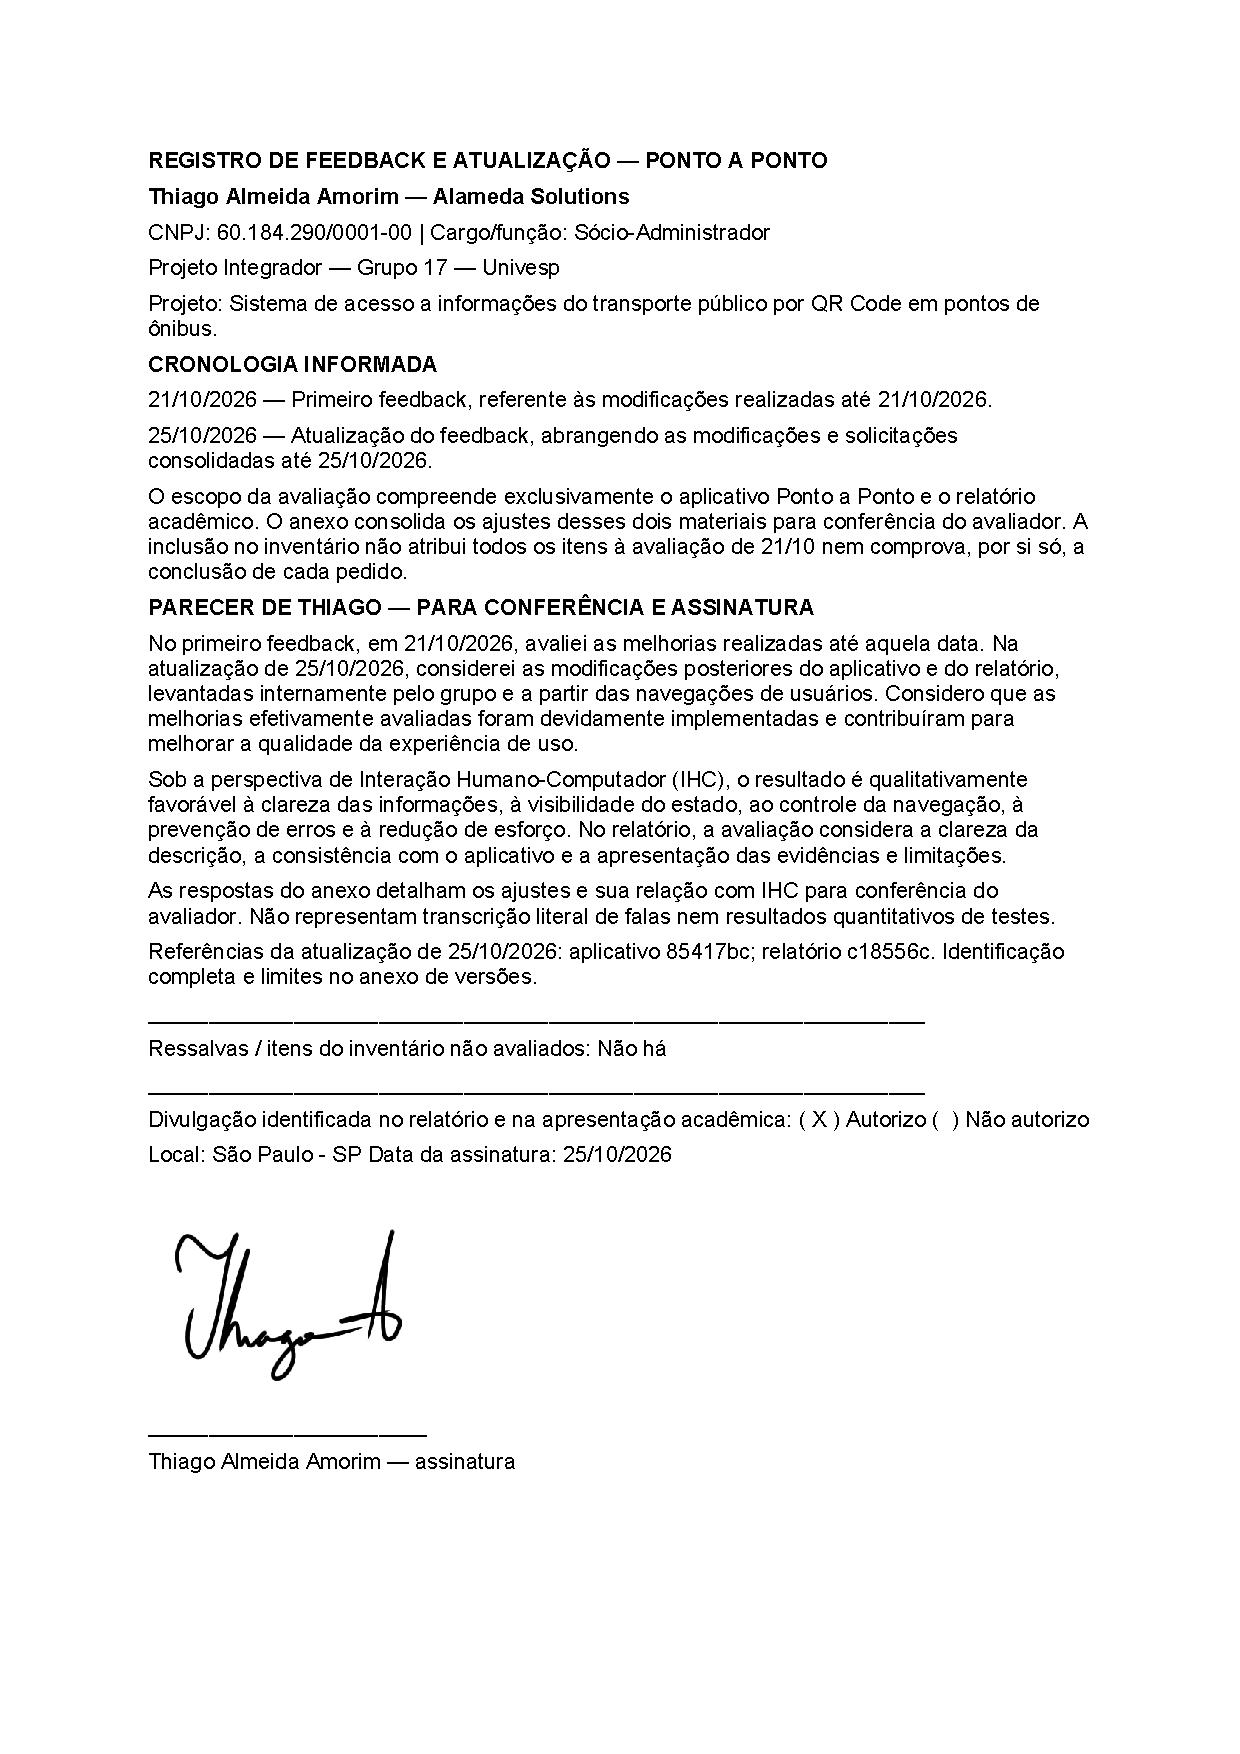
\includepdf[pages=-,pagecommand={\thispagestyle{papnumeracao}},scale=0.95]{avaliacoes_externas/alameda_solutions/documento_confirmado_2026-10-26/Registro_feedback_Thiago_Alameda_Solutions_confirmado.pdf}
\end{anexosenv}

\end{document}
